\documentclass[12pt,openany,oneside]{book}

\usepackage{color}
\usepackage{graphicx}

\usepackage{epstopdf}

\usepackage[square,numbers,sectionbib]{natbib}
\usepackage{chapterbib}
\usepackage[hyphens]{url}

\usepackage{hyperref}
\usepackage{index}
\usepackage[acronym,nopostdot]{glossaries}
\makeglossaries

\usepackage{bookmark}
\usepackage{subfig}

\usepackage{xcolor}
\usepackage{listings}
\usepackage{caption}

\lstset{basicstyle=\footnotesize\ttfamily,frame=shadowbox,captionpos=b,rulesepcolor=\color{gray}}
\definecolor{notecolor}{RGB}{210,210,210}

\usepackage{float}
\newfloat{Note}{htbp}{note}

\usepackage{fancybox}
\usepackage{wrapfig}


%	\makebox[\linewidth]{\rule{\paperwidth}{0.4pt}}
%	\noindent\rule{\textwidth}{0.8pt}
%	\rule{\textwidth}{0.4pt}
%	\unhbox\mysidebox
%	\begin{wrapfigure}{l}{30pt}
%		\centering
%		
\includegraphics[width=30pt]{pics/tangent-deck}
%	\end{wrapfigure}
%}

%		\begin{minipage}[t]{.1\textwidth}
%			\vspace{0pt}
%			
\includegraphics[width=.5\textwidth]{pics/tangent-deck}
%		\end{minipage}

		%\begin{lrbox}{\mysidebox}
%}{
%		\end{lrbox}

%		\fcolorbox{black}{notecolor}{
%			\begin{minipage}[t]{.85\textwidth}
%				\unhbox\mysidebox
%			\end{minipage}
%		}

%		\begin{lrbox}{\mysidebox}
		%\end{lrbox}

\usepackage{framed}

%XXX possibly create a "pitfall", "warning" box
%XXX possibly turn into a float

\newsavebox{\mysidebox}
\newenvironment{sidenote} {
	\begin{lrbox}{\mysidebox}
}{
	\end{lrbox}
	\begin{wrapfigure}{l}{25pt}
		\centering
		
\includegraphics[width=25pt]{common/pics/tangent-deck}
	\end{wrapfigure}
	\begin{framed}
		\noindent\unhbox\mysidebox
	\end{framed}
}

\newsavebox{\myexpbox}
\newenvironment{experience}
{
	\begin{lrbox}{\myexpbox}
}{
	\end{lrbox}
	\begin{wrapfigure}{l}{30pt}
		\centering
		
\includegraphics[width=30pt]{common/pics/totally-socks-donkey}
	\end{wrapfigure}
	\begin{framed}
		\noindent\unhbox\myexpbox
	\end{framed}
}


\newsavebox{\mytapbox}
\newenvironment{advice}
{
	\begin{lrbox}{\mytapbox}
}{
	\end{lrbox}
	\begin{wrapfigure}{l}{30pt}
		\centering
		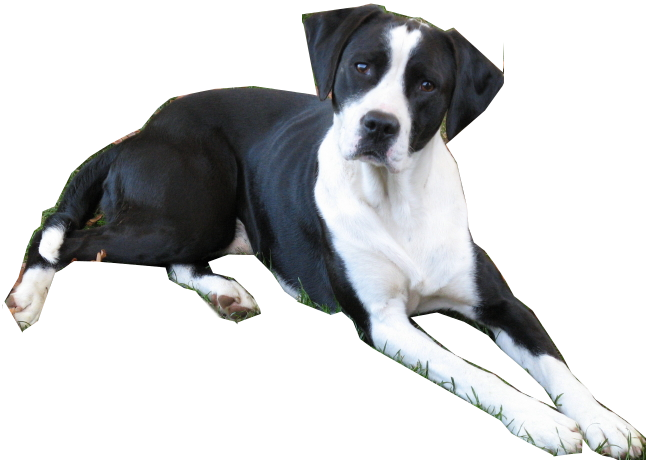
\includegraphics[width=30pt]{common/pics/pointer}
	\end{wrapfigure}
	\begin{framed}
		\noindent\unhbox\mytapbox
	\end{framed}
}




%{
%	\begin{minipage}{.15\textwidth}
%		
\includegraphics[width=.5\textwidth]{pics/tangent-deck}
%	\end{minipage}
%	\begin{lrbox}{mybox}
%}{
%	\end{lrbox}
%	\fcolorbox{black}{notecolor}{
%		\begin{minipage}{.75\textwidth}
%			\usebox{\mybox}
%		\end{minipage}
%	}
%}

\newcommand{\manpage}[1]{{\tt #1}\index{\tt #1}}


\makeindex
\newindex{names}{adx}{and}{Name Index}

\begin{document}

\title{Principles of System Administration}
\author{Jan Schaumann \\
\texttt{jschauma@netmeister.org}}

\maketitle

\tableofcontents
\lstlistoflistings
\phantomsection
\listoffigures
%\listoftables

\newglossaryentry{abi}
{
	name={ABI},
	first={\acrlong{abi} (ABI)},
	long={Application Binary Interface},
	description={{\em \acrlong{acm}} A computer programming
interface provided by libraries, for example.  This interface promises to
the developers a certain behaviour, including the alignment of data types
and calling conventions.  See also: API}
}

\newglossaryentry{acl}
{
	name={ACL},
	first={\acrlong{acl} (ACL)},
	long={Access Control List},
	description={{\em \acrlong{acl}}  A list of
permissions, commonly attached to a network or file resources.
An \acrshort{acm} defines e.g. what privileges are granted to
the object or what sort of network traffic may be
allowed.}
}

\newglossaryentry{acm}
{
	name={ACM},
	first={\acrlong{acm} (ACM)},
	long={Association for Computing Machinery},
	description={{\em \acrlong{acm}}  A learned society for
computing, governing Special Interest Groups, publishing academic journals
and sponsoring numerous conferences.}
}

\newglossaryentry{afp}
{
	name={AFP},
	first={\acrlong{afp} (AFP)},
	long={Apple Filing Protocol},
	description={{\em \acrlong{afp}}   A network file system / protocol
used predominantly by Apple's Mac OS versions (both ``Classic'' and OS X).
Sometimes also referred to as ``Apple Share''.}
}

\newglossaryentry{afs}
{
	name={AFS},
	first={\acrlong{afs} (AFS)},
	long={Andrew File System},
	description={{\em \acrlong{afs}} A distributed network file system
developed at Carnegie Mellon University with certain distinguishing
features over other network file systems, including authentication via
Kerberos, access control lists and, to some degree,
location independence.}
}

\newglossaryentry{api}
{
	name={API},
	first={\acrlong{api} (API)},
	description={{\em \acrlong{api}} A specification
describing the interfaces of a given software component.  This
specification is sufficiently high-level so as to allow the developer of
software using this API to not care about {\em how},
the interface is implemented. See also: ABI},
	long={Application Programming Interface}
}

\newglossaryentry{aws}
{
	name={AWS},
	first={\acrlong{aws} (AWS)},
	long={Amazon Web Services},
	description={{\em \acrlong{aws}} Amazon.com's cloud computing
platform.}
}

\newglossaryentry{bbs}
{
	name={BBS},
	first={\acrlong{bbs} (BBS)},
	long={Bulletin Board System},
	description={{\em \acrlong{bbs}} The electronic version of a
traditional bulleting board and the predecessor of Usenet and,
conceptually, todays Internet ``forums''.}
}

\newglossaryentry{bind}
{
	name={BIND},
	first={\acrlong{bind} (BIND)},
	long={Berkeley Internet Name Domain},
	description={{\em \acrlong{bind}} The most widely used DNS
software, included in various Unix flavors since
4.3BSD.}
}

\newglossaryentry{bios}
{
	name={BIOS},
	first={\acrlong{bios} (BIOS)},
	long={Basic Input/Output System},
	description={{\em \acrlong{bios}} The basic firmware found on
IBM compatible computers, loaded from read-only memory at system startup
and in charge of initializing some of the hardware components before
handing control over to the boot loader.}
}

\newglossaryentry{bsd}
{
	name={BSD},
	first={\acrlong{bsd} (BSD)},
	long={Berkeley Software Distribution},
	description={{\em \acrlong{bsd}} Commonly refers to a number of
UNIX derivatives based on software distributed by the Computer Systems
Research Group of the University of California at Berkeley.  Open Source
versions include NetBSD, FreeBSD and OpenBSD.}
}

\newglossaryentry{chs}
{
	name={CHS},
	first={\acrlong{chs} (CHS)},
	long={Cylinder-Head-Sector},
	description={{\em \acrlong{chs}} An early scheme used to address
individual sectors (or blocks) on a hard drive by identifying their
location on the disk via the given cylinder (or track), the disk's
read-write heads and finally the individual sector.}
}

\newglossaryentry{cifs}
{
	name={CIFS},
	first={\acrlong{cifs} (CIFS)},
	long={Common Internet File System},
	description={{\em \acrlong{cifs}} An application layer network
protocol used predominantly by Microsoft Windows systems as a network file
system and to communciate with other devices, such as shared printers.
Frequently named {\em SMB/CIFS}, as it was derived from SMB.}
}

\newglossaryentry{cli}
{
	name={CLI},
	first={\acrlong{cli} (CLI)},
	long={Command Line Interface},
	description={{\em \acrlong{cli}} A
human-computer interface primarily relying on
text-based input whereby the user types commands into
a terminal or console interface.  The CLI is valued by
System Administrators as being widely more efficient
and flexible than most graphical interfaces.  See
also: GUI}
}


\newglossaryentry{cm}
{
	name={CM},
	first={\acrlong{cm} (CM)},
	long={Configuration Management},
	description={{\em \acrlong{cm}} See SCM}
}

\newglossaryentry{cpu}
{
	name={CPU},
	first={\acrlong{cpu} (CPU)},
	long={Central Processing Unit},
	description={{\em \acrlong{cpu}} The actual
circuitry (e.g. a microprocessor chip) of a computer
performing the arithmetic and logical operations
within a computer, possibly comprising multiple
computing components or ``cores'' and nowadays even
extending to virtual CPUs.}
}
\newglossaryentry{csnet}
{
	name={CSNET},
	first={\acrlong{csnet} (CSNET)},
	long={Computer Science Network},
	description={{\em \acrlong{csnet}} An early network connecting
computer science departments at academic and research
institutions.}
}

\newglossaryentry{csrg}
{
	name={CSRG},
	first={\acrlong{csrg} (CSRG)},
	long={Computer Systems Research Group},
	description={{\em \acrlong{csrg}} A research group at the
University of California, Berkeley, funded by the Defense Advanced
Research Projects Agency to enhance the Unix operating
system.}
}

\newglossaryentry{cvs}
{
	name={CVS},
	first={\acrlong{cvs} (CVS)},
	long={Concurrent Versions System},
	description={{\em \acrlong{cvs}} The at one point perhaps most
popular open source client-server version control system.  (Yes, {\em CVS}
is a {\em VCS}.  One thing we cannot complain about is a lack of
acronyms.)  In recent years, CVS has lost popularity to the Subversion VCS
and newer distributed revision control systems such as
Git.}
}

\newglossaryentry{darpa}
{
	name={DARPA},
	first={\acrlong{darpa} (DARPA)},
	long={Defense Advanced Research Projects Agency},
	description={{\em \acrlong{darpa}} Originally
known as ``ARPA'', this agency of the United States Department of Defense
is probably best known for the development of what ultimately became the
Internet.}
}

\newglossaryentry{das}
{
	name={DAS},
	first={\acrlong{das} (DAS)},
	long={Direct Attached Storage},
	description={{\em \acrlong{das}} A storage system in which the
disk devices are attached directly, i.e. without any network component, to
the server.  See also: NAS, SAN}
}

\newglossaryentry{dsl}
{
	name={DSL},
	first={\acrlong{dsl} (DSL)},
	long={Domain Specific Language},
	description={{\em \acrlong{dsl}} A language developed for a very
specific purpose, such as the configuration of a given piece of software
or the representation of information within a certain
data model.}
}

\newglossaryentry{dns}
{
	name={DNS},
	first={\acrlong{dns} (DNS)},
	long={Domain Name System},
	description={{\em \acrlong{dns}} A hierarchical, distributed system to
map hostnames to IP addresses (amongst other things).}
}

\newglossaryentry{dram}
{
	name={DRAM},
	first={\acrlong{dram} (DRAM)},
	long={Dynamic Random Access Memory},
	description={{\em \acrlong{dram}} A volatile type of computer
storage used for most computers' and laptops' main
memory.}
}

\newglossaryentry{ebs}
{
	name={EBS},
	first={\acrlong{ebs} (EBS)},
	long={Elastic Block Store},
	description={{\em \acrlong{ebs}} Amazon's block-level cloud storage service.  See also: S3}
}

\newglossaryentry{ec2}
{
	name={EC2},
	first={\acrlong{ec2} (EC2)},
	long={Elastic Compute Cloud},
	description={{\em \acrlong{ec2}} Part of Amazon's Web Services, EC2
allows a user to deploy virtual machines or ``compute instances'' on
demand.}
}

\newglossaryentry{fcp}
{
	name={FCP},
	first={\acrlong{fcp} (FCP)},
	long={Fibre Channel Protocol},
	description={{\em \acrlong{fcp}} A high-speed network protocol
primarily used to connect components in a Storage Area Networks.  FCP
allows for a number of different topologies, most notably connections in a
switched fabric.}
}

\newglossaryentry{ffs}
{
	name={FFS},
	first={\acrlong{ffs} (FFS)},
	long={Fast File System},
	description={{\em \acrlong{ffs}} See: UFS}
}

\newglossaryentry{gcc}
{
	name={GCC},
	first={\acrlong{gcc} (GCC)},
	long={GNU Compiler Collection},
	description={{\em \acrlong{gcc}} A suite of
tools comprising a compiler {\em chain} provided by
the GNU project.  Originally referring to the GNU C
Compiler, the tools provided include support for many
different languages, including C++, Objective-C,
Fortran, Java, Ada, and Go.  The C compiler, invoked via the
{\tt gcc(1)} command, is the de-facto standard and
is shipped with most Unix flavors. See also: GNU}
}

\newglossaryentry{gnu}
{
	name={GNU},
	first={\acrlong{gnu} (GNU)},
	long={GNU's Not Unix},
	description={{\em \acrlong{gnu}} The GNU project was founded to provide free
software and aimed to provide a full operating system.  After having
adopted the Linux kernel, GNU/Linux become commonly referred to just as
``Linux'', much to the chagrin of many GNU proponents.  The contributions
of the GNU project, however, should not be
underestimated.  See also: GPL}
}

\newglossaryentry{gpl}
{
	name={GPL},
	first={\acrlong{gpl} (GPL)},
	long={GNU General Public License},
	description={{\em \acrlong{gpl}} A widely used free software license
originally written by Richard Stallman for the GNU Project.  The license
aims to guarantee availability of the source code for the licensed
software as well as any derived works.}
}

\newglossaryentry{gui}
{
	name={GUI},
	first={\acrlong{gui} (GUI)},
	long={Graphical User Interface},
	description={{\em \acrlong{gui}} A
human-computer interface primarily relying on
interactions with the user through e.g. a mouse or
other pointing device, icons, and other visual cues.
See also / contrast with: CLI}
}

\newglossaryentry{hba}
{
	name={HBA},
	first={\acrlong{hba} (HBA)},
	long={Host Bus Adapter},
	description={{\em \acrlong{hba}} A hardware connector, such as a PCI,
PCI-X, or PCIe card, connecting, for example, a storage medium to a host
system.}
}

\newglossaryentry{hdd}
{
	name={HDD},
	first={\acrlong{hdd} (HDD)},
	long={Hard Disk Drive},
	description={{\em \acrlong{hdd}} A data
storage device using magnetic storage, frequently
rotating platters allowing for random access via a
magnetic read-write head.  See also: SDD}
}
\newglossaryentry{http}
{
	name={HTTP},
	first={\acrlong{http} (HTTP)},
	long={Hyper Text Transfer Protocol},
	description={{\em \acrlong{http}} The ubiquitous
application-layer protocol underlying the World Wide Web, allowing for
distributed documents to be linked.}
}

\newglossaryentry{iaas}
{
	name={IaaS},
	first={\acrlong{iaas} (IaaS)},
	long={Infrastructure as a Service},
	description={{\em \acrlong{iaas}} A concept in cloud computing
whereby infrastructure components are deployed and delivered on demand,
frequently by use of virtualization.}
}

\newglossaryentry{iana}
{
	name={IANA},
	first={\acrlong{iana} (IANA)},
	long={Internet Assigned Numbers Authority},
	description={{\em \acrlong{iana}} An organization
responsible for the global coordination of the DNS Root (i.e., maintenance of
the DNS root zones), IP addressing (i.e., overseeing global IP address
allocation to the regional Internet registries), and other Internet
Protocol resources.  See also: ICANN}
}

\newglossaryentry{icann}
{
	name={ICANN},
	first={\acrlong{icann} (ICANN)},
	long={Internet Corporation for Assigned Names and Numbers},
	description={{\em \acrlong{icann}} A
non-profit corporation overseeing Internet-related tasks, such as the
operation of the IANA.}
}

\newglossaryentry{ieee}
{
	name={IEEE},
	first={\acrlong{ieee} (IEEE)},
	long={Institute of Electrical and Electronics Engineers},
	description={{\em \acrlong{ieee}} A
non-profit professional organization for the advancement of technological
innovation.  Publishes countless journals, leads the creation of many
standards etc.  Some overlap between the IEEE Computer Society and the
ACM.}
}

\newglossaryentry{ietf}
{
	name={IETF},
	first={\acrlong{ietf} (IETF)},
	long={Internet Engineering Task Force},
	description={{\em \acrlong{ietf}} An open, volunteer-based
organization responsible for the development and creation of Internet
standards.  See also: ISOC}
}

\newglossaryentry{iot}
{
	name={IoT},
	first={\acrlong{iot} (IoT)},
	long={Internet of Things},
	description={{\em \acrlong{iot}}
A term describing the internetworking of devices,
especially consumer products, previously typically not
expected to be connected to the internet.  Such
devices are frequently referred to as ``smart''
devices, despite their tendency to be poorly secured
and with questionable functionality deriving from
their ability to connect to -- and be reached from --
the public internet.}
}

\newglossaryentry{ip}
{
	name={IP},
	first={\acrlong{ip} (IP)},
	long={Internet Protocol},
	description={{\em \acrlong{ip}} The fundamental protocol underlying the
Internet, routing datagrams across networks.  Together
with the \acrlong{ip}, the suite is commonly referred
to as {\em TCP/IP}. See also: TCP, UDP}
}

\newglossaryentry{ipc}
{
	name={IPC},
	first={\acrlong{ipc} (IPC)},
	long={Interprocess Communication},
	description={{\em \acrlong{ipc}} Methods for exchanging data
between related or unrelated processes on one or more
systems.}
}

\newglossaryentry{isoc}
{
	name={ISOC},
	first={\acrlong{isoc} (ISOC)},
	long={Internet Society},
	description={{\em \acrlong{isoc}} An international non-profit
organization providing guidance and direction to Internet related
standards and policy.  Parent organization of the IETF, but contains
additionally a strong focus on education.}
}

\newglossaryentry{iscsi}
{
	name={iSCSI},
	first={\acrlong{iscsi} (iSCSI)},
	long={Internet Small Computer System Interface},
	description={{\em \acrlong{iscsi}} A networking
standard for carrying SCSI commands over IP networks.
See also: IP, SCSI}
}

\newglossaryentry{itil}
{
	name={ITIL},
	first={\acrlong{itil} (ITIL)},
	long={Information Technology Infrastructure Library},
	description={{\em \acrlong{itil}} A set of
practices underlying the first international standard for IT Service
Management, ISO/IEC 20000.  ITIL covers a series of publications focusing
on Service Strategy, Service Design, Service Transition, Service
Operation, and Continual Service Improvement.}
}

\newglossaryentry{jbod}
{
	name={JBOD},
	first={\acrlong{jbod} (JBOD)},
	long={Just a Bunch Of Disks},
	description={{\em \acrlong{jbod}} A term describing a simple storage
configuration where individual disks are made available in the operating
system as separate logical units accessed via separate
mount points.}
}

\newglossaryentry{json}
{
	name={JSON},
	first={\acrlong{json} (JSON)},
	first={\acrlong{json} (JSON)},
	long={JavaScript Object Notation},
	description={{\em \acrlong{json}} An
open standard to describe data
objects using key-value pairs.  Despite its name, the
data format is language independent, and libraries to
process and generate JSON exist for virtually all
common programming languages.
	}
}

\newglossaryentry{lan}
{
	name={lAN},
	first={\acrlong{lan} (LAN)},
	long={Local Area Network},
	description={{\em \acrlong{lan}} A physically
close computer network connecting individual
components on Layer 1 or 2 of the OSI stack. See also:
WAN}
}

\newglossaryentry{lba}
{
	name={LBA},
	first={\acrlong{lba} (LBA)},
	long={Logical Block Addressing},
	description={{\em \acrlong{lba}} A scheme used to address
individual sectors (or blocks) on a hard drive by
iterating over them.}
}

\newglossaryentry{ldap}
{
	name={LDAP},
	first={\acrlong{ldap} (LDAP)},
	long={Lightweight Directory Access Protocol},
	description={{\em \acrlong{ldap}} A common protocol
for accessing directory services, such as username lookups, user
groupings, password storage, and other such data.
Defined in RFC4511.}
}

\newglossaryentry{lisa}
{
	name={LISA},
	first={\acrlong{lisa} (LISA)},
	long={The USENIX Special Interest Group for Sysadmins},
	description={{\em \acrlong{lisa}} A non-profit
organization established to serve the System Administration community.
See also: LOPSA.}
}

\newglossaryentry{lopsa}
{
	name={LOPSA},
	first={\acrlong{lopsa} (LOPSA)},
	long={League of Professional System Administrators},
	description={{\em \acrlong{lopsa}} A non-profit
organization established to advance the profession and practice of System
Administration.  See also: LISA.}
}

\newglossaryentry{lun}
{
	name={LUN},
	first={\acrlong{lun} (LUN)},
	long={Logical Unit Number},
	description={{\em \acrlong{lun}} A numerical identifier for a distinct
storage unit or volume in a Storage Area Network.}
}

\newglossaryentry{lvm}
{
	name={LVM},
	first={\acrlong{lvm} (LVM)},
	long={Logical Volume Manager},
	description={{\em \acrlong{lvm}} A tool or
technique to allocate and manage storage space across
multiple block-storage devices and to present them to
the OS as a virtual block device, possibly increasing
storage capacity or performance. }
}

\newglossaryentry{multics}
{
	name={Multics},
	first={\acrlong{multics} (Multics)},
	long={Multiplexed Information and Computing Service},
	description={{\em \acrlong{multics}} A time-sharing operating system
initially developed in the 1960s in collaboration amongst MIT, General Electric,
and Bell Labs. See also: Unics}
}

\newglossaryentry{milnet}
{
	name={MILNET},
	first={\acrlong{milnet} (MILNET)},
	long={Military Network},
	description={{\em \acrlong{milnet}} The part of the ARPANET designated
for unclassified communications of the US Department
of Defense.}
}

\newglossaryentry{nas}
{
	name={NAS},
	first={\acrlong{nas} (NAS)},
	long={Network Attached Storage},
	description={{\em \acrlong{nas}} A storage model in which disk
devices are made available over the network by a file server to remote
clients.  The file server is running an operating system and maintains the
file system on the storage media; client access the data over the network
using specific network file system protocols.  See
also: DAS, SAN}
}

\newglossaryentry{nfs}
{
	name={NFS},
	first={\acrlong{nfs} (NFS)},
	long={Network File System},
	description={{\em \acrlong{nfs}} A distributed network file system
developed by Sun Microsystems.  NFS has become the de-facto standard in
distributed file systems in the Unix world and is supported by virtually
all NAS solutions.}
}

\newglossaryentry{nnt}
{
	name={NNT},
	first={\acrlong{nnt} (NNT)},
	long={Network News Transfer Protocol},
	description={{\em \acrlong{nnt}} An application-level
protocol used to transport messages or ``news articles'' for Usenet,
conceptually similar to SMTP.}
}

\newglossaryentry{nsfnet}
{
	name={NSFNET},
	first={\acrlong{nsfnet} (NSFNET)},
	long={National Science Foundation Network},
	description={{\em \acrlong{nsfnet}} A network
supporting the initiatives of the National Science Foundation and
initially connecting a small number of supercomputing, later on developed
into a major part of the Internet backbone.}
}

\newglossaryentry{nsi}
{
	name={NSI},
	first={\acrlong{nsi} (NSI)},
	long={NASA Science Internet},
	description={{\em \acrlong{nsi}} A multiprotocol wide area network,
combining a DECnet and a TCP/IP based network (the Space Physics Analysis
Network or SPAN and the NASA Science Network or NSN,
respectively).}
}

\newglossaryentry{os}
{
	name={OS},
	first={\acrlong{os} (OS)},
	long={Operating System},
	description={{\em \acrlong{os}} \empty}
}

\newglossaryentry{osi}
{
	name={OSI},
	first={\acrlong{osi} (OSI)},
	long={Open Systems Interconnection model},
	description={{\em \acrlong{osi}} A conceptual
model characterizing and expanding on the layers
described in the TCP/IP model.  The OSI model
describes seven layers: Physical, Data, Network,
Transport, Session, Presentation, Application.}
}

\newglossaryentry{pata}
{
	name={PATA},
	first={\acrlong{pata} (PATA)},
	long={Parallel Advanced Technology Attachment},
	description={{\em \acrlong{pata}} An interface
standard for connecting storage devices to a host system.  Initially named
{\em ATA}, it was renamed {\em PATA} to avoid confusion with {\em SATA}.
Also frequently referred to as {\em IDE}.}
}

\newglossaryentry{pci}
{
	name={PCI},
	first={\acrlong{pci} (PCI)},
	long={Peripheral Component Interconnect},
	description={{\em \acrlong{pci}} A computer expansion bus
used to attach a hardware device such as an HBA to a computer.  There are
different standards (PCI, PCI Express, PCI-X) providing different speeds
and features. Not to be confused with {\em PCI DSS}.}
}

\newglossaryentry{pcidss}
{
	name={PCI DSS},
	first={\acrlong{pcidss} (PCIDSS)},
	long={Payment Card Industry Data Security Standard},
	description={{\em \acrlong{pcidss}} The
information security standard describing the requirements a merchant needs
to meet in order to accept credit cards.}
}

\newglossaryentry{pola}
{
	name={POLA},
	first={\acrlong{pola} (POLA)},
	long={Principle of Least Astonishment},
	description={{\em \acrlong{pola}} A concept of
precitability in software tools, following which any invocation should not
lead to any surprises by the user.}
}

\newglossaryentry{posix}
{
	name={POSIX},
	first={\acrlong{posix} (POSIX)},
	long={Portable Operating System Interface},
	description={{\em \acrlong{posix}} A family of IEEE
standards defining the common API and (command-line) interfaces, primarily
used by the Unix family of operating systems.}
}

\newglossaryentry{post}
{
	name={POST},
	first={\acrlong{post} (POST)},
	long={Power-On Self Test},
	description={{\em \acrlong{post}} A number of simple routines intended
to ensure that the hardware is not obviously faulty, run by most server
systems immediately after the system is powered on and before the boot
loader is run.}
}

\newglossaryentry{pxe}
{
	name={PXE},
	first={\acrlong{pxe} (PXE)},
	long={Preboot eXecution Environment},
	description={{\em \acrlong{pxe}} A combination of protocols
that allow a computer to determine its network information and boot media
dynamically so as to allow for bootstrapping the system over the network.
This process is also known as {\em pxebooting}.}
}

\newglossaryentry{radius}
{
	name={RADIUS},
	first={\acrlong{radius} (RADIUS)},
	long={Remote Authentication Dial In User Service},
	description={{\em \acrlong{radius}} A network
protocol allowing clients to be managed with regards to authentication,
authorization, and accounting via a central service.}
}

\newglossaryentry{raid}
{
	name={RAID},
	first={\acrlong{raid} (RAID)},
	long={Redundant Array of Independent Disks},
	description={{\em \acrlong{raid}} A storage
technology that allows multiple disks to be combined into a single data
container upon which a file system can be created.  Different schemas allow
for increased data redundancy or I/O performance at the cost of decreased
capacity.}
}

\newglossaryentry{rest}
{
	name={REST},
	first={\acrlong{rest} (REST)},
	long={REpresentationsl State Transfer},
	description={{\em \acrlong{rest}} A software architecture
granting distributed access to an object model.  As the name suggests, the
focus is on relaying a given object's current {\em state} See also: SOAP}
}

\newglossaryentry{rfc}
{
	name={RFC},
	first={\acrlong{rfc} (RFC)},
	long={Request For Comments},
	description={{\em \acrlong{rfc}} Publications outlining Internet
related technologies, research, protocols etc.  Some of the RFCs may
become actual {\em standards}; many of them are de-facto standards.}
}

\newglossaryentry{sdd}
{
	name={SDD},
	first={\acrlong{sdd} (SDD)},
	long={Solid State Drive},
	description={{\em \acrlong{sdd}} A
storage device using non-volatile Flash memory to
store data.  See also: HDD}
}
\newglossaryentry{s3}
{
	name={S3},
	first={\acrlong{s3} (S3)},
	long={Simple Storage Service},
	description={{\em \acrlong{s3}} Amazon's object-level cloud storage
service.  See also: EBS}
}

\newglossaryentry{san}
{
	name={SAN},
	first={\acrlong{san} (SAN)},
	long={Storage Area Network},
	description={{\em \acrlong{san}} A network providing access to disk
devices on the block level.  The storage is made accessible to remote
clients on a block level; clients can then create a file system on top of
these storage blocks.  See also: DAS, NAS}
}

\newglossaryentry{sata}
{
	name={SATA},
	first={\acrlong{sata} (SATA)},
	long={Serial Advanced Technology Attachment},
	description={{\em \acrlong{sata}} An interface
standard for connecting storage devices to a host system using high-speed
serial cables.  See also: PATA}
}

\newglossaryentry{scsi}
{
	name={SCSI},
	first={\acrlong{scsi} (SCSI)},
	long={Small Computer System Interface},
	description={{\em \acrlong{scsi}} A set of standards for
physically connecting and transferring data between computers and
peripheral devices.  Interfaces for using SCSI are numbersome and range
from so-called ``Fast SCSI'' (parallel) to Fibre
Channel.  See also: iSCSI}
}

\newglossaryentry{scm-cm}
{
	name={SCM},
	first={\acrlong{scm} (SCM)},
	long={Software Configuration Management},
	description={{\em \acrlong{scm}} The task of maintaining
changes to a computer system's runtime configuration without manual
intervention.  SCM systems are able to install software, update existing
or create new files, or run commands across large numbers of servers.
Some systems include support for non-traditional host systems, including
networking equipment.  Examples of popular SCM systems are: CFengine,
Chef, Puppet.}
}

\newglossaryentry{scm}
{
	name={SCM},
	first={\acrlong{scm} (SCM)},
	long={Source Control Management},
	description={{\em \acrlong{scm}} The task of tracking changes
during software development.  Often referred to as {\em revision control},
performed by a {\em Version Control System}, (VCS).  Examples include CVS,
Subversion, Perforce and Git. To avoid confusion with Software
Configuration Management, we will use the acronym VCS when referring to
source control management.}
}

\newglossaryentry{smb}
{
	name={SMB},
	first={\acrlong{smb} (SMB)},
	long={Server Message Block},
	description={{\em \acrlong{smb}} See CIFS.}
}

\newglossaryentry{sla}
{
	name={SLA},
	first={\acrlong{sla} (SLA)},
	long={Service Level Agreement},
	description={{\em \acrlong{sla}} An agreement between service
consumers and providers, outlining the expecations the users of the
service may pose and that the provider is obligated to meet.  Examples
include maximum turnaround time until an issue is resolved, maximum
downtime of a service or minimum throughput or
bandwidth etc.}
}

\newglossaryentry{smtp}
{
	name={SMTP},
	first={\acrlong{smtp} (SMTP)},
	long={Simple Mail Transfer Protocol},
	description={{\em \acrlong{smtp}} An application-level
protocol used to exchange electronic messages, or email, amongst mail
servers.}
}

\newglossaryentry{snmp}
{
	name={SNMP},
	first={\acrlong{snmp} (SNMP)},
	long={Simple Network Monitoring Protocol},
	description={{\em \acrlong{snmp}} The industry standard
protocol used for monitoring network devices, computer, printers and all
sorts of other systems.}
}

\newglossaryentry{soap}
{
	name={SOAP},
	first={\acrlong{soap} (SOAP)},
	long={Simple Object Access Protocol},
	description={{\em \acrlong{soap}} A protocol used by many
web services to exchange structured information over HTTP using XML.  See
also: REST}
}

\newglossaryentry{spof}
{
	name={SPOF},
	first={\acrlong{spof} (SPOF)},
	long={Single Point of Failure},
	description={{\em \acrlong{spof}} A common term describing a
crucial system component without which nothing works.  Note that
{\em people} can easily become a Single Point of Failure if they retain
exclusive knowledge about the system infrastructure or the internal
details of a given program.}
}

\newglossaryentry{sre}
{
	name={SRE},
	first={\acrlong{sre} (SRE)},
	long={Site Reliability Engineering},
	description={{\em \acrlong{sre}} A term
describing the merging of software engineering with
traditional ``operations'' or system administration,
in many ways similar to the term ``DevOps''.  The term
is believed to originate at Google.
	}
}

\newglossaryentry{ssl}
{
	name={SSL},
	first={\acrlong{ssl} (SSL)},
	long={Secure Sockets Layer},
	description={{\em \acrlong{ssl}} The predecessor to TLS, initially
developed by Netscape.  To this day, TLS and SSL are used interchangeably,
even though TLS has superseded SSL.}
}

\newglossaryentry{tacacs+}
{
	name={TACACS+},
	first={\acrlong{tacacs} (TACACS)},
	long={Terminal Access Controller Access-Control System Plus},
	description={{\em \acrlong{tacacs+}} A remote authentication protocol often used for network equipment,
allowing routers and switches, for example, to communicate with a central
authentication server.}
}

\newglossaryentry{tco}
{
	name={TCO},
	first={\acrlong{tco} (TCO)},
	long={Total Cost of Ownership},
	description={{\em \acrlong{tco}} In software engineering, the total
cost of ownership provides an estimate of what it takes to build or run a
system.  This includes the initial development or purchase cost as well as
the ongoing cost (both monetary as well as in human resources) to
maintain, update, patch and debug the software.}
}

\newglossaryentry{tcp}
{
	name={TCP},
	first={\acrlong{tcp} (TCP)},
	long={Transmission Control Protocol},
	description={{\em \acrlong{tcp}} One of the fundamental protocols underlying the
Internet, routing datagrams across networks.  Together
with the \acrlong{ip}, the suite is commonly referred
to as {\em TCP/IP}.  TCP provides for reliable,
connection-oriented connections between e.g. a server
and a client.  See also: IP, UDP}
}

\newglossaryentry{tls}
{
	name={TLS},
	first={\acrlong{tls} (TLS)},
	long={Transport Layer Security},
	description={{\em \acrlong{tls}} A protocol to allow for
encryption of network traffic on the application layer, currently defined
in RFC5246.  TLS was initially based on SSL, with which it is frequently
used interchangeably.}
}

\newglossaryentry{udp}
{
	name={UDP},
	first={\acrlong{udp} (UDP)},
	long={User Datagram Protocol},
	description={{\em \acrlong{udp}} A transport
layer protocol (i.e. operating on layer 3 of the
TCP/IP model, layer 4 of the OSI model), which allows
for connectionless, unreliable communications between
two endpoints.  See also: IP, TCP}
}

\newglossaryentry{uefi}
{
	name={UEFI},
	first={\acrlong{uefi} (UEFI)},
	long={Unified Extensible Firmware Interface},
	description={{\em \acrlong{uefi}} A specification
defining the interactions between an Operating System and lower-level
firmware.  See also: BIOS}
}

\newglossaryentry{ufs}
{
	name={UFS},
	first={\acrlong{ufs} (UFS)},
	long={Unix File System},
	description={{\em \acrlong{ufs}} A widely adopted file system across
different Unix versions, implementing boot blocks, superblocks, cylinder
groups, inodes and data blocks.  Also called the Berkeley Fast File System
(FFS).}
}

\newglossaryentry{unics}
{
	name={Unics},
	first={\acrlong{unics} (Unics)},
	long={Uniplexed Information and Computing Service},
	description={{\em \acrlong{unics}} The
original name of the UNIX operating system, a pun on
``Multics''.}
}

\newglossaryentry{vcs}
{
	name={VCS},
	first={\acrlong{vcs} (VCS)},
	long={Version Control System},
	description={{\em \acrlong{vcs}} A
component of software and configuration management,
allowing for the tracking of revisions made to a given
set of files.  See also: CVS, SCM}
}

\newglossaryentry{vfs}
{
	name={VFS},
	first={\acrlong{vfs} (VFS)},
	long={Virtual File System},
	description={{\em \acrlong{vfs}} An abstraction layer providing
applications with a consistent interface to different underlying
file systems.  Initially developed by Sun Microsystems.  The term {\tt
vnode} indicates this heritage.}
}

\newglossaryentry{vps}
{
	name={VPS},
	first={\acrlong{vps} (VPS)},
	long={Virtual Private Server},
	description={{\em \acrlong{vps}} A virtual machine provided by a
hosting company to customers.  Payment models range from hourly to monthly
or longer subscriptions.}
}

\newglossaryentry{wan}
{
	name={WAN},
	first={\acrlong{wan} (WAN)},
	long={Wide Area Network},
	description={{\em \acrlong{wan}} A computer
network spanning wide-ranging regions, possibly
connecting different \acrlong{lan}s, designed to
overcome physical proximity requirements. See also: LAN}
}

\newglossaryentry{xml}
{
	name={XML},
	first={\acrlong{xml} (XML)},
	long={eXtensible Markup Language},
	description={{\em \acrlong{xml}} A markup
language based on free, open standards that is frequently
used in web services or by system tools to
describe complex configuration attributes of a
service.}
}


\frontmatter
\chapter{Preface to the preface}

This ``book'' is not (yet) a book.  It is incomplete,
a works in progress.  But given the lack of headway
I've made, and considering the time and effort I have
already invested, I have come to the conclusion that
it's preferable to publish what I have and worry about
finishing the remainder another time.

Since I began working on this project back in 2011, a
lot has changed in the industry as well as in the
SysAdmin class on which this book is based.  You may
find references or topics to be outdated or seem
quaint (although hopefully not obsolete).  I remain
hopeful that the lessons and examples continue to be
applicable, even if details or specific technologies
may continue to evolve.

As time goes by, I may come back to update chapters
I've previously made available.  As such, this text
may change in content, style, available formats, and
organization.  It is even possible that updates are
already available at \\
\noindent {\tt https://www.netmeister.org/book/}.
In the mean time, I welcome suggestions, corrections,
contributions, criticism, and any and all commentary at
{\tt jschauma@netmeister.org}.  \\

\noindent
Jan Schaumann \\
New York, January 14, 2019

\addvspace{.5in}
\noindent
{\em This draft last updated: \\
\today}

\chapter{Preface}

The book you are holding is intended to cover the
broad topic of ``{\em System Administration}'' from a
conceptual point of view with a particular focus on
the foundation of systems administration in a large
scale context.  While the book will pay attention to
Operating System specific details -- in particular the
Unix family of operating systems -- it does not
provide step-by-step instructions, such as  how to set
up a mail server or how to run a monitoring system.
Instead, the basic underlying principles and the
factors that help decide how to best set up a system
for a given purpose will be the topic of discussion.

Wherever possible, case studies and real world
examples based on my own experiences in both small and
large environments will be used to illustrate the
lessons learned.

\section*{Why another book on System Administration?}

Like a lot of Open Source software, this book was
written to ``scratch a specific itch''.  In
particular, I was in need of a suitable course book as
a companion to my class ``Aspects of System
Administration'', which I have been teaching at
Stevens Institute of Technology\index{Stevens
Institute of Technology} since 2005.  The class was
developed to give students a broad overview of the
profession and expose them to the many different
practical aspects, but not to teach specific
individual technologies that would soon be obsolete or
replaced by the next generation.  The breadth of the
topic required that the class focused on fundamental
underlying principles rather than implementation
details.

A significant problem with teaching System
Administration in an academic setting derives from in
the fast-paced nature of the Information
Technology\index{Information Technology} (IT) world.
Curricula and degree programs take a long time to be
developed, reviewed and approved.  By the time a new
textbook has been published, the technology described
may have already become obsolete.

Most existing books relating to System Administration,
thorough and useful as they are, have a practical
"howto" approach or are targeted towards people
already in the profession.  They provide detailed
instructions for various specific problems or discuss
different implementations of a given software service
across different operating systems.

This book is different.  It focuses on {\em concepts}
and the understanding of the given topics on a
fundamental level, so as to facilitate the learning of
how to build scalable solutions that are flexible
enough to adapt to different system requirements.

\section*{Who should read this book}

This book was primarily written to address the lack of
a general purpose course book on the broad topic of
System Administration for my own class.  As such, the
target audience consists of both instructors,
teachers, professors as well as, most importantly,
students.  Because of the wide range of material
covered, some prior knowledge of common
computer-related topics is required, including a basic
understanding of TCP/IP, operating system and file
system concepts, user-level experience using a Unix
like operating system and proficiency in at least one
programming language.

As a graduate level course book, the target audience
may of course also include people with some prior
experience in System Administration.  Their background
will help them take the concepts and topics presented
to the next level and apply the lessons learned in
their own environment.

\section*{Organization of the book}

The outline of this book follows the syllabus of my
class.  The class, in turn, was developed as a series
of lectures covering complex computer systems from the
bottom up.  That is, we begin with more low level
concepts such as storage devices and file systems and
work our way up a stack of layers (including OS and
software installation, multi-user basics and
networking) until we have well understood, networked
and easy to maintain general purpose system, before we
dive into the maintenance of special purpose services.

This book is therefore divided into three major parts.
We begin with an introduction to the profession of
System Administration and the approach taken in this
book.  Next, we cover a number of fundamental
technologies and concepts; this part makes up the bulk
of the content, and each chapter is intended to
accompany or complete a single lecture.  Suggested
exercises, problems or topics of discussions are
included wherever suitable. Finally, we conclude in
the third part with a brief review and a look ahead
into the future direction of System Administration,
both the teaching as well as the professional practice
thereof.

Throughout each chapter we will pay special attention
to three areas: {\em Scalability}, {\em Security} and
{\em Simplicity}.  These three related and at times
overlapping features can be seen as pillars of
professional system design.  Without them, no solution
is complete.  Neither can be added after the fact; all
three have to be integral components of a system's
architecture.

While in general there is some order to the chapters,
you may find yourself flipping back and forth once you
arrive in Part \ref{part:services}, as it builds on
the previous chapters.  One exception to the overall
ordering of chapters may be the chapter on system
security, Chapter \ref{chap:security}.  It should come
as no surprise that the various fundamental
technologies covered in Part \ref{part:fundamentals}
all include references to topics discussed in more
detail in that chapter.

While I have attempted to provide an overall structure
and flow to the topics covered in this book, please
feel free to pick and choose topics based on your
interest or course needs.  Each chapter is, as much as
possible, self-contained to allow you to assign
reading or exercises as you see fit.

\begin{sidenote}
{\bf Notes, Digressions, Tangents} \\
At times we will include ``supplementary'' or rather loosely related
information that is too large for footnotes but not important enough to be
included in the actual text.  Such content will be displayed in boxes like
this close to the most relevant paragraph.  In order to trick the casual
user into actually reading the box, it is accompanied by the entirely
unrelated graphic of a surfboard, Channel Islands' ``The Tangent by Kelly
Slater''.
\end{sidenote}

\begin{advice}
{\bf Advice for instructors} \\
As a course book, we sometimes include advice for instructors.  Such
advice might be a suggestion how to integrate the subject
matter in the class room, an experience report about something that
helped students in the past, or a pointer to supplementary information.
Such advice will be presented in a box like this.  The rather adorable dog
accompanying this box is, of course, a pointer.
\end{advice}

\begin{experience}
{\bf Anecdotes from experience} \\
Sometimes we will illustrate important lessons with practical examples,
experience reports or anecdotes.  These short stories serve to relate the
theoretical material covered to the so-called ``real world''. \\[10pt]

Such anecdotes will be presented using a box like this.  The graphic
intended to lure you into reading the content is a sock puppet, much like
the ones commonly used to entertain children with an educational story of
sorts.  This particular sock puppet happens to be a donkey because I like
to remind myself that despite initial subjective impressions to the
contrary it is usually I who turns out to be the ass.  Some of these
anecdotes will prove this point.
\end{experience}


\section*{Conventions}

A lot of ink and many more innocent bits have been
wasted on the difference of the terms
``\textsc{UNIX}\textregistered{}\index{UNIX}'',
\textsc{UNIX}, ``Unix'', and ``unix-like''.  For the
purpose of this book it hardly warrants further
distinction anymore: all such systems discussed in
this text and used for examples are ``a kind of Unix''
(though few will actually be certified by The Open
Group\index{The Open Group} and thus be allowed to
call themselves \textsc{UNIX}\textregistered).  These
include the various Open Source\index{Open Source}
implementations and derivatives such as the
BSD\index{BSD} family or Linux\index{Linux} (itself
trademarked, by the way).  We will use the term
``Unix'' to refer to these different systems.

If we have to distinguish between the ``Linux''
operating system and other ``Unices'' (the plural we
shall avoid), we will follow common convention and
simply call the operating system technically
consisting of the Linux kernel and all additional
software -- much of it provided by or derived from the
\glslink{gnu}{GNU} Project\index{GNU!Project} -- as
``Linux'' rather than ``GNU/Linux\index{GNU/Linux}''.
\\

We shall also adopt the custom of referring to
specific Unix commands by way of writing the name
followed in parenthesis by the section of the manual
pages in which the command is described.  That is, a
reference to the {\tt stat(1)} command differs from a
reference to the {\tt stat(2)} system call; the
documentation for either can be found by providing the
section number to the {\tt man(1)} command, e.g.: {\tt
man 2 stat}.

% XXX: bold face interesting things?
\begin{lstlisting}[float,label=code:sample,caption=Sample command-line invocations]
$ whoami
jschauma
$ su
Password:
# whoami
root
# exit
$
\end{lstlisting}

This book contains a number of code examples and
listings of commands to be executed at the shell
prompt.  To distinguish between commands entered as a
regular user and commands entered as the superuser, we
use a different prompt following general Unix
convention: a {\tt \$} denotes a user prompt, a {\tt
\#} a superuser prompt.  Listing \ref{code:sample}
illustrates this. \\

The English language does not require a gender to be
assigned to the ``System Administrator''; however, we
need to use a personal pronoun if we wish to refer to
a person holding such a job title.  Consistent use of
only a single gender pronoun might raise the
impression that the duties can only be performed by a
member of that gender, which of course is entirely
absurd.

Since any attempt at using ``he/she'', ``(s)he'' or
any variation is doomed to become nothing but
distracting, we use either ``he'' or ``she'' in
examples in this book.  No suggestion of gender
inequality is intended in any of the examples. \\

Operating systems are distributed by different kinds
of organizations.  Some have commercial backing;
others are provided by a team of volunteers.  Some
software is provided free of charge, other software
requires payment of licensing fees.  Some includes the
source code, some does not -- and either may be the
case for both commercially licensed or freely
available software.  For simplicity, we will use the
terms ``vendor'' or ``provider'' in either case when
referring to the entity distributing the software.

\section*{Examples and Exercises}

As a course book for a graduate level class, the
recommended way to follow the material presented is by
completing (some of) the examples and exercises
included in most chapters.

I have found it invaluable to provide students access
to an environment in which they can create different
server instances running different operating systems
on demand.  At the same time, the nature of many of
the exercises demand unfettered access to the systems
themselves as well as to the network.  This is
something that is nearly impossible to achieve in a
traditional university environment -- had a faculty
member approached me requesting such access for her
students while I was a System Administrator at Stevens
Institute of Technology, I would have balked and
dismissed the request as hardly feasible.

However, a flexible Infrastructure as a
Service\index{Infrastructure!As a Service} (IaaS)
environment such Amazon's \gls{ec2}\index{AWS!EC2} or
other VPS hosting companies overcomes these hurdles;
non-commercial solutions to this problem, such as the
``Virtual Unix Lab''\cite{pre:feyrer-vul} for example,
exist as well.  My own teaching experience has been
supported by Amazon's ``AWS in Education'' research
grants\cite{pre:aws-grant}; as a result, a number of
exercises will reference the EC2 service, but it is
entirely reasonable to perform then in another
environment that provides similar services.  In many
cases, virtualization software installed on a
regular workstation or laptop allowing students to
create virtual instances of different OS is fully
sufficient for many exercises as well. \\

The job of a System Administrator routinely requires
self-guided research, analysis and meticulous
documentation of one's practices and procedures.  To
enforce these practices, many of the assignments,
problems and exercises in this book do not have a
simple right-or-wrong answer.  Just as in real life,
we frequently need to find {\em an} answer and then
determine if the solution we derived is suitable, even
though other equally correct solutions may exist.

To this end, I have made it a habit of requiring
students to search any and all information materials
available to them -- including, but not limited to
their course book(s), library materials, online
newsgroups and forums, websites and the Internet at
large -- and to allow them to use such materials so
long as they properly cite their resources.

\subsection*{Systems}

Practical exercises usually target the Unix family of
operating systems, where they focus on exposing
students to multiple variations of any given system.
I usually assign exercises to be done on the following
operating systems, where possible:

\begin{itemize}
	\item {\em Linux} -- different distributions allow for valuable
		insights into different solutions to the same problem and
		frequently illustrate the point that one system running
		``Linux\index{Linux}'' may behave rather differently from another.
		To this end, I usually pick a Red Hat related distribution
		(Fedora, CentOS) and at least a Debian based distribution
		(Debian or Ubuntu).
	\item one of the {\em BSD}s -- as a developer of the NetBSD\index{NetBSD}
		operating system, I'm of course partial to this particular
		variant, but any one from this lineage will suffice to
		illustrate the genetic Unix heritage.
	\item {\em Solaris\index{Solaris}} -- now freely available as derivatives
		of the unfortunately short-lived OpenSolaris project or
		available as the commercial original version,
		this system is ``different enough'' from the more common Linux
		distributions to provide a good comparison.
\end{itemize}

Even though the general concepts of System
Administration apply across all operating systems and
even across administrative domains such as support for
a large number of desktop systems versus large
deployments of servers in datacenters, we will focus
primarily on the large scale installations and
infrastructure components.  As a result, and due to
the significantly different philosophies and practical
means by which these systems are maintained, we
explicitly exclude Mac OS X and the Windows family of
operating systems as a target platform for
assignments.  Doing so allows us to not get distracted
by implementation details and fundamental platform
differences and to instead focus on internalizing the
principles and lessons explained.


\subsection*{Programming Assignments}

Programming assignments are normally checked on the
university's systems.  I seldom specify the language
in which students have to write their programs.  This
reflects the real-world scenario, where languages are
not usually dictated and the objective is first and
foremost to ``get the job done''.  A few select
exercises may specify the programming language to use;
there is usually an explicit or implicit requirement,
or the implementation in one language lends itself to
better illustrate the lessons learned.

Programming assignments are usually graded not only by
functionality, but also by code quality, user
interface and other factors.  A demonstrated
understanding of the three core pillars --
Scalability, Security, Simplicity -- is essential.
Frequently the assignments will target these criteria,
if at times as hidden requirements.

The practice of giving students maximum liberty in
their research also extends to programming
assignments.  Students are allowed -- encouraged, in
fact -- to search for solutions and reuse existing
code, to collaborate and discuss possible approaches
amongst each other.  It should be noted, though, that
as in their workplace, students need to make sure to
have permission to (re)use the code in question and to
properly credit the origin.  I have found that this
distinction between lifting code found on a website
without acknowledgment and deriving your own solution
from an attributed reference has become harder for
students to make, which is all the more reason to
encourage responsible research.

I believe that this freedom to work as one would under
``normal'' circumstances teaches awareness of code
licensing and improves the student's research skills.
Frequently, the most important part of a successful
homework submission is not the functionality of the
program itself, but the required accompanying
documentation, which illustrates the student's problem
solving progress.

\section*{Acknowledgements}

My biggest thanks go out to the late Prof. Lawrence
Bernstein\index[names]{Bernstein, Lawrence}, formerly
of Bell Laboratories, my former Computer Science and
Software Engineering professor, an IEEE and ACM fellow
and an industry expert on Trustworthy Computing.
Throughout my career, I have found myself going back
to the lessons he tried to teach me, the examples he
gave, the direction he provided.  Larry is the reason
all of these words have eventually come into existence
and been put into a semi-coherent form:

\begin{quote}
How about writing a book? If you follow your class
notes it is not a burden.
\end{quote}

This message came out of the blue back in February of
2011.  After a few emails going back and forth, life
intervening, my second daughter being born, and me
generally trying to figure out how to approach such a
project, I eventually signed a contract with Wiley \&
Sons to actually write this book.

The fact that I never actually completed the work and
eventually withdrew my agreement with Wiley \& Sons
notwithstanding, I remain humbled by the confidence
and encouragement I received from Prof. Bernstein.  I
deeply regret not having been able to complete this
work before he died on November 2nd, 2012.  Thanks for
being a great teacher, Larry!
\\

I have received a lot of feedback on the various
chapters making up this book from many people in the
industry over the years.  I appreciated all the help
given by friends and colleagues, with particular
thanks to those having reviewed drafts of the
different chapters:
Subbu Allamaraju,
Mohit Chawla,
Jennifer Davis,
Peter Ellehauge,
Patrick Debois,
Hubert Feyrer,
Al Hoang,
Kevin Kempton,
Tom Limoncelli
James K. Lowden,
Jan Lehnardt,
Daria Mehra,
Marc Farnum Rendino,
Kimo Rosenbaum.

Many thanks to Amazon for granting my students ample
AWS usage credits.  Without access to EC2, many of the
exercises in this book would not be possible.
\\

Finally, and as expected, my deepest thanks to my wife
Paula and my daughters Ana and Sofie, without whom, as
many a famous dedication goes, this book would have
been completed much, much earlier.  I may still get
there.


\pagebreak
\bibliographystyle{plainnat}
\begin{thebibliography}{99}

\bibitem{pre:feyrer-vul}Hubert Feyrer, {\em System Administration Training in
the Virtual Unix Lab - An e-learning system with diagnosis via a domain
specific language as base for an architecture for tutorial assistance and
user adaption}, Shaker Verlag GmbH, Aachen, Germany, 2009. ISBN
978-3-8322-7874-8.

\bibitem{pre:aws-grant}{\url https://aws.amazon.com/education/}

\end{thebibliography}


\mainmatter
\part[Introduction and General Concepts]
{Introduction and General Concepts}
\label{part:introduction}

\chapter[Introduction]
{An Introduction to System Administration}
\label{chap:introduction}

\begin{quote}
{\em system administrator, n.}:\\
one who, as a primary job function, manages computer and network systems
on behalf of another, such as an employer or client.\\
\end{quote}

\begin{figure}[hb]
	\raggedleft
	
\includegraphics[width=.25\textwidth]{01/pics/we-are-happy-to-serve-you-coffee-mug}
	\caption[Anthora Coffee Cup]{System Administrators: well
		caffeinated and always happy to serve you.
		\label{fig:we-are-happy-to-serve-you}}
\end{figure}

\section{What exactly does a System Administrator do?}
\label{introduction:introduction}

Every semester I start my class with this simple
question: ``What exactly does a System Administrator
do?''  My audience consists of undergradate and
graduate students of Computer Science or Computer
Engineering; some of them have experience working as a
System Administrator or IT support (either part-time
or full-time), while others may maintain their own
home network or otherwise perform some of the tasks
commonly associated with the job of a System
Administrator.  Some may have no practical experience
in this area, but all do have an idea of what the job
entails.

As a result, the responses are varied, ranging from
very specific (``Use \verb+tcpdump+ to troubleshoot
network problems.'') to the more general (``Maintain
the network.''), quickly illustrating that there is no
one concise description of the professional duties of
System Administrators; rather, we identify a number of
tasks that are expected to be performed by people
holding this title.  The broad range of these tasks --
especially when put in context of the size and goals
of different organizations and their deployment
footprint -- makes obvious the fact that a System
Administrator in one company may not do the same thing
as one in a different company.  In fact, even within a
single organization we usually find that two people
may well both be called ``SysAdmin'', but perform
rather different duties.

So what {\em does} a System Administrator do?  It
seems that most people agree that this job has to do
with computers in some capacity, but that really is
already where the definitions start to become fuzzy:
System Administrators are in charge of ``servers'' as
well as of personal computers, desktop machines,
laptops and, increasingly, mobile devices.  With the
evolution of computing coming full circle, we find
that the migration from the mainframe computer to the
personal and independent computing device to the
networked server back to the central {\em
Infrastructure as a Service}\index{Infrastructure!As a
Service} model inherent in today's Cloud
Computing\index{Cloud Computing} concepts places the
System Administrator in the middle of it all.

So perhaps the main focus of a System Administrator's
job is then really the central connection between the
independent systems, the network itself?  Hmmm, System
Administrators surely are involved in the deployment
and installation of the computers in a datacenter (or
is that the task of specific Datacenter Technicians?)
and connecting all the different components certainly
involves a lot of cables.  But then, don't we have
{\em Network} Administrators, or is that a more
specialized subcategory of System Administrators?

System Administrators seem to spend as much time
typing cryptic commands into dark terminal windows as
they do running cables and labelling hardware, and
while they may no longer shuffle punch cards, they
frequently do write programs to help them complete
their tasks.  System Administrators are known to get
woken up in the middle of the night when things go
``bump'', and as a result they are also known to have
a fondness for caffeinated drinks.  They are able to
kickstart a generator, assess the required cooling
power for their server room, use duct tape in creative
and unexpected ways, assemble servers out of
mysterious looking parts, and may end up handling a
circular saw or other heavy machinery when their
Leatherman multi-tool cannot complete the task.

System Administrators plan, budget and design networks
and backup or storage systems, add and delete users
(well, user {\em accounts}, anyway\footnote{There is a
strong love/hate relationship between System
Administrators and their users.  Much as the SA may
joke that they wish they could make users disappear,
without users the systems they are in charge of
might well hum along uninterrupted, but would
ultimately be entirely useless.}), install and update
software packages, draft policy documents, fight spam
with one hand while rebuilding a corrupted revision
control\index{revision control} system with the other.
They have access to all systems in the organization,
may undergo retina- and fingerprint scanners to access
``Mission Impossible''-style protected datacenters and
spend countless hours in front of a multitude of
computer screens, typing away on oddly shaped
keyboards consuming not entirely healthy amounts of
coffee and energy drinks.

Well... in some places, a System Administrator might
do all of this.  In others, there might be different,
more specialized people for the various tasks:  there
might be datacenter technicians and ``SiteOps'',
Network Administrators, System Programmers, System
Architects, Operators, Service Engineers, Storage
Engineers, \glslink{sre}{Site Reliability
Engineers}\index{SRE}, Virtual Operations,
Infrastructure Architects... the number of different
job titles for things that might otherwise fall into
the more general ``SysAdmin'' category seems endless.

The various areas of expertise included in the day to
day routine such as system design, infrastructure
architecture, system fault diagnosis, hardware
benchmarking, and others eventually require experience
in a number of related fields; a lot of them involve
more than just a little bit of programming experience
and in some cases complex infrastructure tools based
on solid software engineering practices need to be
built.  This illustrates that just as it is hard to
clearly define where System Administration begins, we
often can't quite put our finger on where it ends and
another discipline becomes the primary job function.

Even if job descriptions and duties differ
significantly, there are a lot of people who simply
identify as {\em System Administrator} regardless of
job title.  We all have something in common: {\em we
manage and maintain computer and network systems}.

\begin{experience}
{\em A typical bug} \\

At one place of employment we had a tool that would
add users to a given host by gathering the login
information for all the users, \verb+ssh(1)+ to each
host and update \verb+/etc/passwd+ using the host's
native tools (such as \verb+useradd(8)+, etc.). Many a
system administrator has written a similar tool, and
for the most part, this program worked reasonably
well. (We will discuss how to better manage user
accounts across large numbers of machines later in
this book.) \\ [10pt]

But all software fails eventually, and for one reason
or another I had to debug the tool. Groveling through
a few hundred lines of perl that had clearly been
written by different people in different stages of
their career, I came across a code block that included
the following call: \\ [10pt]

\verb+chmod(0666, "/dev/null");+ \\ [10pt]

Asking around, it became clear that {\em somehow} some
of the systems ended up in a state where
{\tt /dev/null}\index{\tt /dev/null} was unreadable
or -writable by normal users, which leads to a number
of complications.  But nobody had been able to track
down just how exactly this happened until one day we
were lucky enough to witness the change in
permissions,  but the only activity by a user with
sufficient privileges to make such a change was a
\verb+sudo(8)+ invocation of \verb+less(1)+. \\
[10pt]

\verb+less(1)+ happens to make use of a history file
to remember search commands between invocations, much
like your shell may use a history file (such as
\verb+~/.bash_history+). \verb+less(1)+ is aware of
the fact that the history file might contain sensitive
information, and it actively changes the permissions
on that file to only allow read/write access to the
owner.  But for the root user, we explicitly symlinked
all common such history files to \verb+/dev/null+ to
avoid accidental leaking of secrets to disk. \\ [10pt]

And therein lies the bug: \verb+less(1)+ was invoked
by the super user, it would check the permissions on
the file \verb+/root/.lesshst+, follow the redirection
to \verb+/dev/null+, find that they're not \verb+0600+
and call \verb+chmod(2)+, yielding and
unreadable/unwritable \verb+/dev/null+.  We were able
to confirm this behaviour and identified a code change
in later versions of \verb+less(1)+ that fixed this
problem. \\ [10pt]

Understanding such failures and identifying their root
causes requires a deep understanding of the operating
system and its tools, but tracking down bugs like
this\cite{intro:devnull} is just one of the many
aspects of a System Administrator's daily routine.

\end{experience}

\section{The Profession of System Administration}
\label{introduction:profession}

Most professions have a fairly clear and formal
definition as well as an obvious career path and
background requirements.  In fact, for a person to
take on a particular line of work, it frequently is
a requirement to undergo a specific, regulated
education, to perform a certain amount of practical
training (such as an apprenticeship), to subscribe to
specific professional ethics\index{ethics} and
guidelines, and eventually to obtain a license to
practice the given profession.  Doctors, scientists
and lawyers all have well-defined professions, as do
engineers of most disciplines.\footnote{Software
Engineering, another young discipline related to
System Administration and technically a specialized
branch of Computer Engineering, differs in that it
does {\em not} have strict licensing regulations.
Anybody can call themselves a ``Software Engineer'',
just as anybody can call themselves a ``System
Administrator''.}

System Administration, on the other hand, does not
(yet) have any of the criteria given above: there is
no specific, regulated training, and as we have seen
in Section \ref{introduction:introduction} not even
agreement on what precisely the job definition ought
to be.  The \gls{lisa}\index{USENIX} attempts to fill
this void to some degree by providing for an informal
but professional community.  Still, due to the nature
of the changing environment, any attempt to create a
concise job description invariably fails by resorting
to very general terms.  Consider the following
description given by the Buerau of Labor
Statistics\cite{intro:bls}:

\begin{quote}
{\em Systems administrators} design, install, and
support an organization's computer systems. They are
responsible for LANs, WANs, network segments, and
Internet and intranet systems. They work in a variety
of environments, including large corporations, small
businesses, and government organizations. They install
and maintain network hardware and software, analyze
problems, and monitor networks to ensure their
availability to users. These workers gather data to
evaluate a system's performance, identify user needs,
and determine system and network requirements.
\end{quote}

While this captures {\em in general} the common job
duties of a System Administrator, it does not answer
the question we asked initially: Just what {\em
exactly} does a System Administrator do?

In order to better grasp the generic description, I've
found it useful to break down the title into its
components, {\em System} and {\em Administrator}.
What, then, is a ``System''?  Any dictionary will give
you a reasonable definition along the lines of:

\begin{quote}
{\em system, n}: A group of interacting, interrelated,
or interdependent elements that together form a
complex whole.
\end{quote}

In this context we will focus on {\em computer-human
systems}\cite{intro:burgess-analytical} consisting of
any number of computing devices, the network(s)
connecting them, the users utilizing these resources,
and of course the impact of the goals of the
organization running such systems.

What about ``Administrator''?  Merriam-Webster's
Collegiate Dictionary defines the term ``to
administer'' as:

\begin{quote}
{\em administer, v}: to manage or supervise the
execution, use, or conduct of
\end{quote}

The profession\index{System Administration!Profession}
of System Administration should therefore be described
as one in which practitioners ``manage or supervise
the execution, use, or conduct of a group of
interacting, interrelated, or interdependent
computer-human elements'', leaving us, in terms of
specificity, about where we began!  We find slightly
more formal definitions of actual job titles, desired
skills and a rather useful distinction between ``small
uniform'', ``complex'', and ``large and complex''
sites in the \gls{lisa} booklet ``Job Descriptions for
System Administrators''\cite{intro:lisa-jobs}, but in
searching for a suitably clear definition of the
profession, we realize that the formal education as a
System Administrator is almost completely lacking.

Job descriptions and postings normally list a degree
in Computer Science or Computer Engineering as
``desirable''; more frequently you will find a
requirement expressed as ``BS, MS or PhD in Computer
Science or equivalent work experience''.  Computer
Scientists will wonder just how, exactly, ``work
experience'' can be mapped, treated as equivalent to
their formal education -- all too often, ``Computer
Science'' in this context is equated with ``knows how
to program, understands TCP/IP''.

As invaluable as actual hands-on experience is, it is
no substitute for a formal degree in the area of
Computer Science.  (Nor is having such a degree a
substitute for practical experience.) Rare is the
candidate who can fully understand the average and
worst-case runtime of his or her programs and scripts
without having learned Big-O Notation; rare the system
programmer who completely grasps the elegance of
modularization provided by, say, function pointers
without having learned the $\lambda$-calculus.
Becoming a proficient System Administrator without
this background is certainly possible, but it makes it
significantly harder to advance beyond a certain
level.

Be that as it may, the focus on many years of
real-world experience as the primary qualification is
both cause and effect.  In the past, there really
existed {\em no} formal training whatever: technically
skilled people found themselves in the position of
being the go-to guy to fix the computers, to make
things work.  Perhaps they ended up working with a
more senior administrator in a sort of informal
apprenticeship, but for the most part their skills
were learned by experience, through trial by fire.
The lack of any formal program in this area
necessitates and then further encourages
self-learning, and many things simply can only really
be understood by experience.  It's a clich\'{e}, a
platitude that you learn the most from your worst
mistakes -- it is also entirely true.

As a result, many of the senior people in hiring
positions do not have an academic background and are
hesitant to require what was not available then to
fill current openings.  System Administrators are also
still frequently treated as -- and at times view
themselves as fulfilling -- a ``janitorial'' role.  If
no industry standard exists by which to measure a
candidate's accomplishments in the field, how can we
require formal education for a job that eludes
definition in the first place?

Therein, however, lies a fallacy.  Practical
experience and formal training do not make up for one
another; they complement each other.  It {\em is} true
that we learn the most from our worst mistakes (and
thus need a chance to make them); it is {\em also}
true that we frequently are only {\em able} to learn
due to a deeper understanding of the problem.  \\

The profession of System Administration is incredibly
interesting precisely {\em because} it eschews a fixed
definition, a formal governing body, a static career
path, or a licensing exam.  It attracts and invites
interesting people from all sorts of backgrounds; it
allows phenomenal potential for job growth and it is
-- must be, due to the advances in the industry --
fast-paced and continually evolving.  But it has
become more mature: professional organizations like
\gls{lisa} have contributed significantly to the
status of the profession by formalizing the
requirements and duties as well as providing a Code of
Ethics\footnote{For a more detailed discussion of both
the (lack of a) definition of the profession and the
ethical obligations we face, please refer to
\cite{intro:primum-non-nocere}.}, and over the last
few years more and more universities have started to
offer classes and degree programs in this area.

System Administrators may not need to be licensed by a
central board anytime soon -- and people will continue
to argue about whether or not that is desirable or
even possible in this field -- but what a few years
ago still was best described as ``a job'' certainly
has grown up to become a career, a craft, a {\em
profession}.

\section{System Administration Education}
\label{introduction:education}

System Administration is rarely taught as an academic
discipline in large part due to its perceived
``blue-collar'' status: from the top of the scholarly
ivory tower, it must be hard to distinguish where an
entry-level job like ``Tech Support'' or the ``Help
Desk'' ends and where a profession demanding a
significant background in Computer Science and
Engineering begins.

System Administrators are highly skilled information
technology specialists shouldering significant
responsibility in any organization.  As we discussed
in the previous sections, the variety of job
descriptions and differences in what a System
Administrator actually may be doing make it difficult
to provide simple step-by-step instructions on how to
enter this field.  As a result, System Administration
has long been a profession that is learned primarily
by experience, where people grow into a position in
order to fulfill the requirements of an organization
rather than follow a career path well-defined by
courses, degrees, and meaningful certifications.

The industry has responded by producing a large number
of practical certification exams that hope to attest
to the student's proficiency in the subject matter.
Practically, most of these certifications appear to
primarily test a person's ability to memorize specific
commands, further reinforcing the notion that System
Administration can be reduced to empirical knowledge,
making practical experience indeed equivalent, if not
superior to one of those scholastic degrees.

But certification that one remembers a specific
vendor's unique configuration file syntax does not
imply actual {\em learning} has taken place; holding a
one-week ``boot camp'' -- the name itself is revealing
of it's educational intention --  to drill enough
information into the participants' heads such that
they pass an exam at the end of the week does not
guarantee long-term retention of that knowledge.
Furthermore, there is no oversight of the topics
taught in such classes, no review of suitability or
correctness.

System Administrators who excel at their jobs do so
not because they have accumulated arcane tribal
knowledge about obscure pieces of hardware and odd
software systems (useful as that is), but because they
understand fundamental underlying principles and
combine that knowledge with their concentrated
experience.

System Administration -- its principles, fundamentals
and practice -- should be {\em taught}.  Since you are
reading this book, chances are that you are currently
taking a class in System Administration as a student
or perhaps you are teaching such a class.  But we
cannot teach an entire profession in a single class or
even using a few select courses.  It is necessary to
develop academic degree granting programs that
comprehensively prepare students for the varied and
wide requirements imposed on them when they enter the
industry.  Such programs should be combined with
extensive real-world and hands-on experience wherever
possible, perhaps by including internships,
cooperative education and apprenticeships provided by
industry leaders.  As students you are entitled to
practical and useful exercises; as educators we have an
obligation to create these and make available the
required resources.

We need classes that combine the academic mission of
fostering independent research with the factual
requirements posed by the positions offered in the
marketplace.  We need instructors who have years of
experience in varied environments, who understand the
practical restrictions that may make the ideal
theoretical solution utopian but who are consciously
aware of these boundaries and able to teach their
students the awareness of them.  At the same time, we
need scholars willing to further this profession
through research and build a theoretical body of
knowledge to become the foundation of future programs.

\subsection{Challenges in System Administration Education}
\label{introduction:education:challenges}

Formal classes in System Administration as part of a
Computer Science or Engineering curriculum are still
uncommon, but in the past few years more and more
institutions have recognized the industry's need for
academic courses that adequately prepare students for
the multitude of responsibilities within this field
and have started to offer such classes (and in some
cases complete degree programs).  But the history of
this profession brings with it a number of unique
challenges when it comes to formally teaching its
principles and practices.

To really understand and appreciate some of the most
general aspects of System Administration, you need to
be exposed to actual running systems.  Practical
experience is so integral to this profession that it
cannot be separated from the theoretical knowledge and
postponed until the student enters his or her first
job or apprenticeship.  But therein lies a significant
hurdle to traditional teaching methods: students need
to administer a system, to have superuser access, to
have a chance to configure a system for a specific
service, and to make the kind of spectacular mistakes
that experienced System Administrators value (if only
in hindsight).

This normally conflicts with the requirements of the
IT department at your university: students would
require access to a number of different OS when the
school's system administrators strive for a certain
level of homogeneity. In order to understand OS
installation concepts, file system tuning, and other
low-level principles, students need to perform these
tasks themselves. Learning to debug network
connectivity issues or being able to actually see the
payload of captured network traffic requires access to
raw sockets, which the staff responsible for the
security of the campus network would certainly rather
not provide.

After years of struggling to give all students equal
access to the resources required for the diverse
assignments and frequently having to change the
assignments to be able to make use of available
resources, I finally decided to do what many companies
do: I outsourced the resource provision problem into
``the Cloud'' -- specifically, to Amazon's
\gls{ec2}\index{AWS!EC2}\footnote{In
this book, I will frequently make reference to or cite
examples from this experience.  At the same time, I
also will suggest exercises that cannot be done in a
cloud environment and that may require access to
dedicated hardware.}.\cite{intro:login-teaching-sa}
Similar results can be achieved by granting students
access to a dedicated laboratory environment or by
providing another on-demand infrastructure via
virtualization of the local compute resources.  If you
are a student, it is worth your time to investigate
all possible resources available to you; if you are an
instructor, consult with your IT department as to the
availability (or perhaps development) of such systems.
\\

But teaching System Administration should also combine
the practical elements noted above with topics from
other academic fields.  As an area of specialization,
System Administration fits in well within the current
Computer Science curricula, since the profession's
requirements draw heavily from many of the same
subjects.  Shared requirements include Operating
Systems, Networking, Database Systems, Distributed
Systems, Cryptography and of course Software
Engineering; at the same time, System Administrators
benefit from deep insights in Computer Architecture
and Systems Engineering as well as Project Management
and of course ``the 5 elements of administration''
(Planning, Organizing, Command (directing people),
Coordination, Control, also listed as
Budgeting)\cite{intro:wiki-fayolism}, usually covered
in Business Administration classes.

To advance the practice of System Administration, the
two existing professional organizations \gls{lisa} and
the \gls{lopsa} are already promoting best practices
and important communities.  Still, we are missing
strong proponents of System Administration as an
academic discipline\footnote{Mark Burgess, previously
of the Oslo University College in Norway, one of the
only universities offering a Master's degree in
Network and System Administration, deserves explicit
mention as one of the few exceptions.} But there are
more and more of us who believe that it's time for the
profession to be recognized as both requiring a
theoretical background in addition to extensive
practical experience and benefitting from the
opportunities of dedicated research opportunities and
the development of universally accepted degree
granting requirements.  Some even write books to
further this goal...

\section{The Three Pillars of Exceptional System Design}
\label{introduction:pillars}

More than just maintain computers and infrastructure
components, System Administrators control entire
systems.  With more experience and seniority, they are
ultimately in charge of building these systems, of
designing the infrastructure and its components so
that the job title frequently morphs into that of a
Systems or Network ``Architect''.  It seems that
people can't help but draw parallels to the so-called
``real'' world, where engineers and architects have
well defined roles (and status).  This does not come
as a surprise; as Brooks\cite{intro:brooks-design}
illustrates masterfully, the parallels between
designing and building a house, a computer or a
complex piece of software are plentiful.

Billy Hollis\index[names]{Hollis, Billy} points
out\cite{intro:hollis} that the title of the
``Software Architect'' is a misleading analogy, that
the duties traditionally performed by people holding
this title are much more akin to those of a structural
engineer than those of a (traditional) architect.  The
role of the System Administrator is likewise
frequently comparable to that of the structural
engineer in the mechanical world, but the advanced
senior System Administrator -- who ultimately steps
into the role of planning, designing and overseeing
the construction of complex systems -- might better
known as ``Systems Architect''.  Structural systems
engineers are then needed to aide in the final design
and implementation of the system in question.

Conceiving of and designing systems as complex as
those System Administrators are in charge of, with
their myriad pieces, the unpredictable human element
and the rather unfortunate tendency of computers to do
precisely what they were instructed to do rather than
what we intended them to do requires expert in-depth
knowledge in a broad range of topics.  Exceptional
System Administrators are generalists -- they have
been trained in a wide area of topics, deepened their
understanding of several and perhaps have become
subject matter experts in a few, but ultimately back
into a role that allows them to apply their ability to
connect the dots, to see the big picture and the
connections between and effects of multiple systems on
each other.  They are well-equipped to model new
components of an infrastructure or to redesign a
system from scratch to meet the new requirements.

For a system to be suitable both for the immediate
requirements today and for a few years down the road,
when the current needs have changed, it must embody
two basic principles: Scalability and Security.
Neither of these can be added to a system after it has
been built:  trying to apply ``security'' after the
system interfaces have been defined yields
restrictions, limitations; trying to make a system
with inherent limitations perform under circumstances
it was not designed for yields hacks and workarounds
-- the end result frequently resembles a fragile house
of cards more than a solid reliable structure.

The third fundamental feature of expertly designed
systems, Simplicity, is simultaneously obvious and
counter-intuitive.  Simplicity underlies both
scalability and security, since reduced complexity
implies better defined interfaces, minimized ambiguity
in communications or data handling and increased
flexibility.  As with the other two core aspects,
simplicity cannot be added after the fact; it must be
inherent in the architecture.  Simplicity is the
enabler of both scalability and security.

An exceptional system exhibits inherent structural
integrity (another wonderful analogy to the world of
bricks and mortar), and this integrity is provided by
these three pillars.  Our focus on these components
may initially seem arbitrary: meeting requirements
across different teams with different priorities has
long been the bane of many a program manager due to
each team focusing on different qualities, of which we
could have picked any number.  However, upon more
detailed analysis and with some years of experience we
have time and again found Simplicity, Security and
Scalability to be the core qualities enabling a
harmonious development- and deployment process.

Throughout this book, we will analyze the systems we
discuss with special focus on these crucial criteria.
You will find that we will frequently talk in broad
abstracts or surprising detail about the implications
of our design decision.

\subsection{Scalability}
\label{introduction:pillars:scalability}

In recent years, the word ``scalability'' has become
one of the defining requirements for virtually all
technical solutions.  Providers of infrastructure
services and products throw it around in an attempt to
impress their customers by how much load their systems
can handle.  It typically seems near synonymous with
``high performance'', the ability to handle large
amounts of data, traffic, connections, and the like.
This may be misleading, as people might be inclined to
believe that such capabilities come at no additional
(or incremental or proportional) cost.  In fact,
scalability does not relate to the costs of the
running system, but to its architecture.  A scalable
system may well require additional resources and
throwing money at a problem actually {\em is} a
perfectly viable solution in many cases.  However, a
scalable architecture is one that does not require a
refactoring of the whole system, a restructuring of
{\em how} data is handled based on changing
circumstances.  Instead, it abstracts data from
process flow and simply adapts.

System Administrators frequently suffer from
Goldilocks Syndrome, striving to provide a solution
that is {\em just right}; wasting resources is just as
anathema to their definition of a correct solution as
not providing adaequate capabilities.  Therefore, we
tend to focus not only on the ability to scale {\em
up} -- to accommodate larger amounts of data or more
requests per minute, for example -- but also to scale
{\em down}, to free up unused resources based on the
demands.  As such, our definition of ``scalability''
leans more towards the overall flexible nature of a
scalable system, its ability to adapt to changing
requirements at run time; a term frequently associated
with Cloud Computing, ``elasticity'', perhaps more
aptly describes this feature, yet it fails to quite
capture as well the sense of meeting extreme
requirements.  We shall continue to use the term
``scalability'' for that reason.  \\

While many systems are {\em flexible}, few are able to
handle input or requirements an order of magnitude
different from those initially conceived of when the
system was designed.  In order to accomodate such
changes, systems are said to either scale {\em
vertically} -- that is, one system is able to handle
the added load, possibly by addition of certain
resources (network bandwidth, CPU power, memory, disk
space, ...) -- or to scale {\em horizontally} -- that
is, a single system is replicated and demands are
spread across them evenly.  Either approach has
certain implications on the overall architecture.  For
horizontal scaling to be beneficial, for example, the
problem space needs to be such that a distribution is
both possible and algorithmically feasible.  However,
this adds communication overhead, as interfaces and
data flow becomes more complex.

Whether by vertical or horizontal means, a scalable
system is one that readily adapts to changing demand.
The designer may not know what will be required of it
in the future, but will make choices that permit the
system to grow and shrink without bumping into
arbitrary limits.

We will take a closer look at the implications of this
idea on the software development practices and overall
Unix Philosophy in Chapter \ref{chap:unix}; for the
time being, let us consider the Unix tradition of
simple tools operating on streams of text as a
wonderful example of a clear interface definition.
Anybody developing a tool that accepts input only from
a file restricts the flexibility of the tool; this
frequently goes hand in hand with an implicit
limitation on the amount of data that can be handled
(think maximum file size, buffers frequently allocated
to read in the entire file, the ability to
\verb+seek(2)+ on the file handle, ...).  By choosing
text rather than a binary format, any future use of
the output is not limited by the original author's
imagination of what future users might wish to
accomplish.  Given sufficiently large or, rather,
diverse datasets, building more complex systems that
perform equally well under heavy load using
complicated, yet limited interfaces so frequently
developed by major software companies easily becomes a
frustrating exercise in determining these
boundaries.

But scalability is not only of concern when tools are
developed; as we design infrastructure components, we
need to be acutely aware of the interfaces between
them and what kind of data can flow back and forth.
Frequently we have no control over the input (both
type and amount), so our systems need to be fault
tolerant of many unenvisioned circumstances.  Even
though somewhat counter-intuitive at first, I argue
throughout this book that a robust system will remain
resilient to overall failure by being comprised of
infrastructure components that themselves may fail
quickly (and explicitly) and that such well-defined
behaviour underlies true scalability.

Hindsight being 20/20, scalability related issues
often can be traced back to a lack of imagination or
confidence in the system.  What if our initial use
case increases not by a factor of two or three, but
hundredfold?  Suppose our system is still in use in
five years -- will average input be likely to remain
the same?  In our discussions, exercises and problems
we will encourage students to consider how a system
performs if circumstances and inputs change by an
order of magnitude.  The ability to anticipate
extraordinary change in requirements requires some
practice and experience by the System Administrators
in charge of the infrastructure; reacting in
well-defined ways to such change is one of the core
features of a reliable system, and the principles that
make a system scalable -- fault tolerance, data
abstraction, clearly defined interfaces -- must be
applied at all stages.  We will reinforce these axioms
throughout all chapters in this book.


\subsection{Security}
\label{introduction:pillars:security}

All too frequently, the software or information
technology industry treats system security as an
afterthought, as something that can be added to the
final product once it has met all the other functional
requirements, after the user interface has been
determined and after all code has been written.  It is
then not surprising that the old adage that security
and usability are directly and inversely related seems
to hold true.  Nevertheless, I would argue that the
very problem statement -- ``the more secure you make
something, the less usable it becomes''\footnote{We
will elaborate on the somewhat surprisingly accurate
corrolary that ``The more secure you make something,
the less secure it
becomes.''\cite{intro:norman-security} detail in a
later chapter.} -- reflects a fundamental
misunderstanding, as it implies that usability is
present first and security ``added'' afterwards.

This approach suggests that the only way to reduce
risks is to {\em take away} functionality; but any
time you do that or otherwise restrict the users, they
will either stop using the product/system altogether
or come up with a creative solution that works around
your newly imposed restrictions.  To be effective,
security needs to be built into the system from the
design phase on.  That is, rather than starting out
with a solution that provides the desired
functionality and then attempting to figure out how to
get it to a secure state, we should instead begin with
a secure albeit restricted state and then slowly add
functionality -- without compromising safety -- until
the desired capabilities are available.  That is, we
need to view security as an enabling factor present at
the design's conception.

Much like software, a system infrastructure is usually
developed with much looser an idea of what one wishes
to accomplish than people are willing to admit.  In
order to achieve maximum functionality and the widest
possible use, people tend to design interfaces with
few restrictions.  Often it is the role of the
security-minded engineers to ask questions that
require the developers or designers to revisit their
requirements; proactive security imposes restrictions
on what the system is able to do.  That is a {\em
good} thing!  General-purpose systems are much harder
to design than special-purpose sytems (``Constraints
are friends''\cite{intro:brooks-design} allow-lists
provide significantly better and more reliable
security than deny-lists).

Any parent can tell you that it is nearly impossible
to take away a toy from a child, even if the toy has
not been used in months or years.  The very idea of
something being taken away seems to trigger in people
(of all ages) a ``but I might need it some day''
response.  Giving users access to a resource (network
access, disk space, physical access, CPU power, ...)
is trivial -- restricting the use once access has been
granted is near impossible; the genie cannot be put
back into the bottle.  It is therefore imperative to
understand precisely what level of access to what
resources you {\em actually} need and not build a
system for the most widest possible use.  Well defined
-- restricted -- small components can still provide
the flexibility to build scalable systems, but each
component needs to be designed from the beginning with
security in mind.  Just as a chain is only as strong
as its weakest link, an infrastructure is only as
secure as its most open or exposed component.  \\

Rare is the software developer who dismisses
``security'' as of minor importance, yet this mythical
property everybody pays at least lip service to has an
incredibly wide definition and may mean different
things in different contexts.  Generally speaking, we
require {\em risk management} (we discuss this in more
detail in a later chapter); more specifically we will
look at a number of computer-human system specific
aspects of security such as (but not limited to):

\begin{itemize}
	\item Cryptography\index{cryptography}, and the three main features that allow
		it to help mitigate risks:
		\begin{itemize}
			\item Secrecy or Confidentiality
			\item Accuracy or Integrity
			\item Authenticity
		\end{itemize}
	\item Physical Security
	\item Service Availability
	\item Service Design
	\item Social Engineering and other aspects of human nature
	\item Trust
\end{itemize}

Throughout this book, we will allude to these
components wherever appropriate, and we encourage
students to come up with possible threat scenarios as
a regular exercise.  Establishing and fostering a
proactively defensive, some may say ``paranoid'',
mindset is an important element of a System
Administrator's development.  Knowing that we cannot
provide an all-encompassing mantle of security after
the system has been designed (much less deployed!), we
strive to integrate it in all stages, leading it to
bolster our infrastructure as an inherent feature.



\subsection{Simplicity}
\label{introduction:pillars:simplicity}

As our discussion of scalability and security
suggested, the practical application of these
principles yields a reduction of interfaces,
end-points, use cases and overall variance.  In other
words, scalable and secure systems are less {\em
complex} and -- it is worth drawing this distinction
explicitly -- much less {\em complicated}.  A complex
system may be well-organized and exhibit a clear,
logical structure yet require subtle or intricate
connections or components.  Complicated systems, on
the other hand, are irregular, unpredictable or
difficult to follow.

``Complexity is the enemy.'' This quote has been
repeated endlessly in so many contexts that it can
almost be assumed common knowledge amongst software
engineers, cryptographers and other security
experts\cite{intro:schneier-ce}.  But while many
people in the information technology industry may
agree on this in principle, I have found that, like so
many aphorisms, the translation into the real world --
the actual application of its consequences -- trails
far behind the good intentions.

In the world of System Administration reducing
complexity is particularly difficult.  As we discussed
in Sections \ref{introduction:introduction} and
\ref{introduction:profession}, managing large
computer networks has {\em inherent} complexity:
multiple components must interface with each other in
many ways to help people -- simultaneously the origin
of true entropy as far as computers are concerned and
dangerously predictable -- accomplish their individual
and collective goals.  But it is important to
differentiate between {\em required}
complexity\index{Complexity!essential} and {\em
accidental}
complexity\index{Complexity!accidental}\cite{intro:brooks-mmm}.
We strive to reduce overall complexity by building
ultimately intricate systems out of smaller, simpler
components.

To repeat an almost ubiquitous prime example of how
simplicity enables astounding flexibility and may
allow you to build complex systems, we will time and
again draw the analogy to the concept of toy building
blocks: themselves simple, nearly unbreakable and
available in a reasonably limited number of shapes and
sizes you can build just about anything with them.

Like these little blocks, the Unix operating system
builds on the philosophy of simple tools that ``do one
thing and do it well'', that work together, commonly
by being connected via the ubiquitous pipe,
operating on text
streams\cite{intro:mcilroy-unix-philosophy}.  We aim
for solutions that exhibit comparable elegance.
``Simple'' does not, it should be noted, mean
``trivial'' or ``easy'': it is so much easier to {\em
add} features, to increase the output, to justify
additional input than it is to reduce a component to
its bare necessities.  As Antoine de Saint
Exup\'{e}ry\index[names]{de Saint
Exup\'{e}ry, Antoine},
observed\cite{intro:exupery:terre-des-hommes}:

\begin{quote}
{\em Perfection is reached not when there's nothing left to
add, but when there's nothing left to remove.}
\end{quote}

But how do we design a simple infrastructure?  The
simple answer is: we can't.  The end result will
always be complex.  But the systems we create will be
more fault tolerant, more performant, more flexible
-- in short: better -- if we remember that our
building blocks need to resemble Lego blocks more than
swiss army knifes.  In other words: we design {\em
for} simplicity.  We keep interfaces internally
consistent and logical.  We use simplicity as a
scalpel to cut away the clutter.

The ability to resist the temptation to ``enhance''
your architecture or software tool to implement
additional features that, if at all necessary, might
better be provided by a separate component, usually
only comes with strong will power and years of
experience.  At the same time, simplicity is found to
underly all of the exemplary technologies you are
likely to encounter and some of which we will present
in the coming chapters.  Sometimes it takes a second
look to recognize and appreciate the genius of
simplicity; hopefully this book will help sharpen your
awareness of this trait.

%"Fools ignore complexity. Pragmatists suffer it. Some can avoid it.
%Geniuses remove it." -- Alan Perlis

\section{The Future of System Administration}
\label{introduction:future}

The System Adminstrator's job definition is diverse,
and so is the rather significant change the profession
has undergone over the years.  Gone are the days of
shuffling punch cards, of cycling magnetic tapes, of
connecting your dumb terminals using RS-232 serial
connections, of stringing ribbon cables inside large
computer cases... or are they?

Some things haven't really changed all that much.
Technologies come and go, but certain principles have
remained the same.  Using fibre-optic cables rather
than twisted-pair, using Infiniband or Fibre Channel
instead of Ethernet or parallel \glslink{scsi}{SCSI}, or
using wireless networks instead of physically
connected systems does not fundamentally change the
day-to-day operations.

Virtualization\index{Virtualization} and Cloud
Computing\index{Cloud Computing} may seem to limit the
need of an organization to hire their own System
Administrators, but I believe that rather than a
threat to the profession these technologies are simply
one of the ways in which we make progress as
information technology specialists.  A chapter towards
the end of the book discusses the future direction of
System Administration and revisits these topics as
well as some of the latest trends in how System
Administration intertwines with other disciplines --
the terms ``DevOps\index{DevOps}'' and ``Agile
Infrastructure'' (or ``Agile Operations'') deserve
particular attention in that context.

A few years ago, the Personal Computer signified a
paradigm change away from the central Mainframe
computer accessed remotely by users towards a
distributed storage and compute model.  System
Administrators found themselves supporting more and
more individually powerful connected devices, trying
to centralize certain resources and services such as
shared filespace or regular backups, for example.  In
the recent past, the move towards software and data
storage services ``in the cloud'' has brought the
evolution full circle:  once again, we are challenged
to provide reliable central services that are accessed
by small, though increasingly mobile, devices.

The separation of {\em systems} from {\em networks},
if it ever really existed, is disappearing.
Standalone systems separated from the Internet are
rare; systems operating completely on their own
without {\em any} network connectivity have become
largely impractical.  Does this change the job of the
System Administrator?  Does it make things more or
less interesting, difficult, challenging, exciting,
different?  Will we see another shift back towards a
model where data storage and processing happens again
on the edge nodes of the network?

We don't know.  But we do know this: whatever happens,
System Administrators will be needed.  Perhaps they
will carry a different title and perform different
practical tasks, but the concept of the profession
will remain.  Organizations small and large will need
somebody with the knowledge and experience to analyze,
troubleshoot and design new infrastructures; somebody
who builds and maintains scalable and secure systems;
somebody with an appreciation of the simple things in
life.

\begin{quote}
{\em Plus \c{c}a change, plus c'est la m\^{e}me chose.}
-- Jean-Baptiste Alphonse Karr\index[names]{Karr, Jean-Baptiste Alphonse}
\end{quote}
\vfill

\begin{figure}[hb]
	\includegraphics[width=1\textwidth]{01/pics/Ibm704}
	\caption[An IBM 704 mainframe]{An IBM 704 mainframe.
		With cloud computing coming full
		circle, we already live in the future!
		\label{fig:mainframe}}
\end{figure}

\pagebreak

\chapter*{Problems and Exercises}
\addcontentsline{toc}{chapter}{Problems and Exercises}
\section*{Problems}
\addcontentsline{toc}{section}{Problems}

\begin{enumerate}

\item Create a course notebook (electronic or
otherwise).  In it, write down your notes about each
chapter, add any links to additional information,
noteworthy insights, etc.  After each chapter, write
down lessons learned.  Differentiate between those
directly applicable to you and those you consider
worthwhile reviewing or investigating in the future.

\item Create a folder for your course work as a
central place for all your documentation.  Whenever
you go through practical exercises, make sure to write
down how you solved a specific problem.  Your
documentation will later on help you review the
lessons you learned and can be used as a practical
how-to guide, so make sure to verify all steps before
you write them down.

\item Ask a System Administrator (for example: in your
university, of an open source project you participate
in, at work) to describe their daily routine.  Compare
notes with others.

\item Consider the current most popular websites and
Internet businesses or organizations.  Try to find out
details about their infrastructure and how it is
maintained.

\item Research available classes and degree granting
programs in the field of System Administration.
Compare their contents to those of industry standard
certification courses.

\item Research professional organizations related to
System Administration (such as LISA and
\glslink{lopsa}{LOPSA}).

\begin{enumerate}

\item Review their mission and content and consider
joining their mailing lists.  They provide a great way
to keep up to date with real-world experiences and
itemlems.

\item How do these organizations compare to the
\glslink{acm}{ACM}, \glslink{ieee}{IEEE} or
\glslink{isoc}{ISOC}?

\end{enumerate}

\item Research common Internet standard bodies and
practices.  What is an \glslink{rfc}{RFC}?  What do the
\glslink{ietf}{IETF}, \glslink{iana}{IANA} and
\glslink{icann}{ICANN} do?

\item Consider the systems you have access to: what
are their primary functions, for what goals were they
designed?  Suppose they grew by an order of magnitude
-- what itemlems would you foresee?

\item Consider the systems you have access to: what
kind and how is access granted?  What kind of security
itemlems can you imagine?

\item Research the terms ``DevOps''\index{DevOps} and
``SRE''\glslink{sre}{SRE}.  In how far do the practices it
represents change the typical job description of a
System Administrator?

\end{enumerate}

\section*{Exercises}
\addcontentsline{toc}{section}{Exercises}

\begin{enumerate}

\item
\label{item:basic}
Practice basic system tasks in your virtualized
environment by creating different OS instances and run
them.  Once running, log in on the virtual host and
run the required commands to:

\begin{enumerate}

\item display basic system information (\verb+uname+,
\verb+ifconfig+, \verb+netstat+, ...)

\item
display the partition table

\item
display the currently mounted file systems

\item
display available disk space
\end{enumerate}

\item Repeat Exercise \ref{item:basic} for a different
Unix flavor than what you are used to.  For example,
if you used a Linux instance for Exercise
\ref{item:basic}, repeat it using OpenSolaris or
FreeBSD.

\item Determine the Unix commands you execute most
frequently (for example via analysis of your shell's
history file).  Analyze the top three commands for
their complexity and interfaces.

\item Analyze your interactive shell usage.
\begin{enumerate}

\item Change your login shell for at least a week to
one that you are not accustomed to.  Make note of the
changes in behaviour.

\item Disable tab completion and any aliases you have
defined in your login shell for at least a week.  How
does this change your workflow?

\item Review the detailed documentation of your login
shell's \verb+builtin+s.  Practice the use of those
that you are not familiar with.

\end{enumerate}

\end{enumerate}

\pagebreak

\bibliographystyle{plainnat}
\begin{thebibliography}{99}

\bibitem{intro:devnull}``less bug, more /dev/null'',
Jan Schaumann, on the Internet at
\url{http://is.gd/NpihsH} (visited November 29,
2015)

\bibitem{intro:bls}Bureau of Labor Statistics, U.S.  Department of Labor,
{\em Occupational Outlook Handbook, 2010-11 Edition, Computer Network, Systems,
and Database Administrators}, on the Internet at
\url{http://www.bls.gov/oco/ocos305.htm} (visited December 10, 2011)

\bibitem{intro:burgess-analytical}Mark Burgess, {\em Analytical Network and
System Administration: Managing Human-Computer Systems}, Wiley \& Sons,
2004

\bibitem{intro:m-w}{\em Merriam-Webster's Collegiate Dictionary}, 10th Edition,
Merriam-Webster

\bibitem{intro:lisa-jobs}Tina Darmohray, {\em Short Topics in System
Administration: Job Descriptions for System Administrators}, 3d Edition,
USENIX Association, Berkeley, CA, 2010

\bibitem{intro:login-teaching-sa}Jan Schaumann, ``Teaching System
Administration in the Cloud'' in {\em ;login: The USENIX Magazine},
October 2010, Volume 35, Number 5

\bibitem{intro:wiki-fayolism} {\em Fayol's Elements of Management} on the
Internet at \url{https://en.wikipedia.org/wiki/Fayolism} (visited December
17, 2011)

\bibitem{intro:brooks-design}Frederick P. Brooks, Jr., {\em The Design of
Design}, Addison-Wesley Professional, 2010

\bibitem{intro:hollis} {\em Billy Hollis Still Builds
Apps}, transcript of an interview with Billy Hollis,
``.NET Rocks'', on the Internet at
\url{http://is.gd/Suk2hr} (visited December 23, 2011)

\bibitem{intro:norman-security}Donald A. Norman, ``THE WAY I SEE IT: When
security gets in the way'', in {\em Interactions}, November 2009, Volume
16, Issue 6, ACM, New York, NY

\bibitem{intro:schneier-ce}Niels Ferguson, Bruce Schneier, and Tadayoshi Kohno,
{\em Cryptography Engineering}, John Wiley \& Sons, March 2010

\bibitem{intro:brooks-mmm}Frederick P. Brooks, Kr., {\em The Mythical
Man-Month: Essays on Software Engineering, Anniversary Edition},
Addison-Wesley Professional, Anniversary edition (August 12, 1995)

\bibitem{intro:mcilroy-unix-philosophy}M. D. McIlroy, E. N. Pinson, and B. A.
Tague {\em Unix Time-Sharing System Forward}, The Bell System Technical
Journal. Bell Laboratories, 1978

\bibitem{intro:exupery:terre-des-hommes}Antoine de
Saint-Exup\'{e}ry, {\em Wind, Sand and Stars},
Harcourt, 2002

\bibitem{intro:primum-non-nocere}Jan Schaumann, {\em
Primum non nocere - Ethical Obligations in Internet
Operations}, VelocityConf NYC 2015; on the Internet at
\url{https://www.netmeister.org/blog/primum-non-nocere.html}
(visited January 16th, 2017)

\end{thebibliography}

\chapter{Unix}
\label{chap:unix}

\begin{quote}
{\em {\textsc{UNIX} is basically a simple
operating system, but you have to be a genius to
understand the simplicity.}} -- Dennis
Ritchie\index[names]{Ritchie, Dennis M.}
\end{quote}

\begin{figure}[hb]
	\raggedleft
	
\includegraphics[width=.25\textwidth]{02/pics/unix-plate}
% XXX: no caption but label?
	%\caption{\label{fig:unix-plate}}
	\label{fig:unix-plate}
\end{figure}

\section{Unix History}
\label{unix:history}

%\begin{figure}[b]
%	\captionsetup{justification=justified,singlelinecheck=false}
%	\caption[\textsc{UNIX} License Plate]{Live Free or Die - UNIX
%		\label{fig:unix-plate}}
%\end{figure}


For many people the term ``System Administrator''
implies operation of Unix systems, even though the
same concepts, tasks and practices apply largely to
the maintenance of hosts running any operating system.
In this book, we strive to describe principles that
are universally applicable and not bound by a specific
operating system.  We will regularly use Unix as the
prime example and cite its features and specific
aspects because of its academic background, long
history of openness, high penetration of the
infrastructure marketplace, and its role as
a cornerstone of the Internet.

\subsection{The Operating System}
\label{unix:history:os}

How the Unix operating system came to be and how that
relates to the development of the Internet and various
related technologies is fascinating; just about every
other Unix-related book already covers this topic in
great detail.  In this chapter, we summarize these
developments with a focus on the major milestones
along the road from the birth of Unix as a test
platform for Ken Thompson's ``Space Travel'' game
running on a PDP-7\index{PDP-7} to the most widely
used server operating system that nowadays also
happens to power consumer desktops and laptops (in the
form of Linux and Apple\index{Apple}'s  OS X\index{OS
X}), mobile devices (Apple's iOS\index{iOS} is OS X
based and thus Unix derived; Google\index{Google}'s
Android\index{Android} is a Linux\index{Linux}
flavor), TVs, commodity home routers, industry scale
networking equipment, embedded devices on the
\gls{iot}\index{Internet of Things}, and virtually all
supercomputers\footnote{TOP500\cite{history:top500}, a
project ranking the 500 most powerful computers in the
world, listed over 89\% as running a version of Linux
or Unix.}.  We will pay attention to those aspects
that directly relate to or influenced technologies
covered in subsequent chapters.  For much more
thorough and authoritative discussions of the complete
history of the Unix operating system, please see
\cite{history:bell-labs-unix-history},
\cite{history:dmr-history} and
\cite{history:esr-taoup} (to name but a
few).\footnote{The ``Unix Heritage Society'' mailing
list\cite{history:tuhsml} is another particularly
noteworthy resource in this context.  It continues to
be an incredible source of historical, arcane, and yet
frequently and perhaps surprisingly relevant
information and discussions around the history of the
Unix family of operating systems.  It is notable for
the regular participation of many of the original
developers and researchers from the early days of
Unix.} \\

Let us briefly go back to the days before the  Unix
epoch\index{Unix!epoch}.  Unix keeps time as the
number of seconds  that have elapsed\footnote{It is
worth adding that this does not include leap seconds,
thus making Unix time a flawed representation of what
humans like to refer to as linear time.  Leap seconds
are inserted rather unpredictably from time to time,
and Unix time has to be adjusted when that happens.
Worse, {\em negative} leap seconds are possible,
though have never been required.  Just more evidence
that Douglas Adams\index[names]{Adams, Douglas} was
right: ``Time is an illusion, lunch time doubly
so.''\cite{history:adams-h2g2}} since midnight UTC of
January 1, 1970, also known as ``POSIX
time''\footnote{This is also the reason why, for
example, Spam\index{Spam} with a ``Sent'' date set to
{\tt 00:00:00} may, depending on your timezone offset
from UTC, show up in your inbox with a date of
December 31, 1969.}.  The date was chosen
retroactively, since
``\glslink{unics}{Unics}\index{Unics}'' -- the {\em
Uniplexed Information and Computing Service}, as the
operating system was initially called\footnote{The
name was a pun on the
``\glslink{multics}{Multics}\index{Multics}'' system,
an alternative for which it was initially developed
as.} -- was created by Ken
Thompson\index[names]{Thompson, Ken}, Dennis
Ritchie\index[names]{Ritchie, Dennis M.}, Brian
Kernighan\index[names]{Kernighan, Brian W.}, Douglas
McIlroy\index[names]{McIlroy, Douglas} and Joe
Ossana\index[names]{Ossana, Joe} in 1969. That is,
Unix predates the {\em Unix epoch}!

It is interesting and a testament to the clean design
to see that the basic functionality and interfaces of
an operating system developed over 40 years ago have
not changed all that much.  The  C\index{C}
programming language was developed in parallel by
Dennis Ritchie\index[names]{Ritchie, Dennis
M.}\index[names]{Kernighan, Brian
W.}\cite{history:kr}, for and on Unix.  Eventually,
Unix itself was rewritten in C, and the programming
language became such an integral part of the operating
system, such a fundamental building block, that to
this day no System Administrator worth their salt can
avoid learning it, even though nowadays most tools
running on top of Unix are written in higher-level,
often interpreted languages.

The structure of the Unix file system, which we will
revisit in much detail in Chapter \ref{chap:file
systems}, the basic commands available in the shell,
the common system calls, I/O redirection, and many
other features remain largely unchanged from the
original design.  The concept of the pipe\index{pipe},
which defines and represents so much of the general
Unix philosophy, was first implemented in
1973\cite{history:mcilroy-reader}, and we still
haven't figured out a better, simpler, or more
scalable way for two unrelated processes to
communicate with each other.

Since its parent company  AT\&T\index{AT\&T} was
prohibited from selling the operating
system\footnote{Under a ruling stemming from an
anti-trust settlement in
1958\cite{history:esr-taoup}, AT\&T was only able to
commercially sell Unix after divesting itself from
Bell Labs.}, Bell Laboratories\index{Bell
Laboratories} licensed it together with the complete
source code to academic institutions and commercial
entities.  This, one might argue, ultimately led
directly to the very notion of ``Open
Source\index{Open Source}'' when the \gls{csrg} of the
University of California, Berkeley, extended the
operating system with their patchsets, which they
called the ``\acrlong{bsd}'' or BSD.

Likewise, the licensing of this ``add-on'' software
allowed Berkeley Software Design Inc. (BSDI) to
develop and sell their operating system BSD/OS.  This
lead directly to the famous
lawsuit\cite{history:bsdisuit} by Unix System
Laboratories (USL), a wholly owned subsidiary of AT\&T
/ Bell Labs, who did not appreciate BSDI selling their
operating system via the 1-800-ITS-UNIX number.  It
has been argued that this lawsuit eroded some
companies' confidence in the BSD family of operating
systems and caused them to adopt a new Unix clone
called ``Linux\index{Linux}'' despite its more onerous
license.  Regardless of the ``what if''s involved,
this part of the history is rich in lessons ranging
from business logic and legal impact of software
licensing to the psychological impact of version
numbering and other aspects of software product
release.\footnote{For the rather interesting
details, including the full ruling of the courts as
well as many discussions around its repercussions,
please see the references at the end of this chapter
-- the legal battle and its impact on the history of
computing alone could fill a book.}

The different direction taken by the \gls{csrg} and the
commercial entities which licensed and then sold the
Unix operating system and the evolution of the code as
it was merged between these branches ultimately lead
to two main directions: the BSD derived family of
systems and the ones tracing back to (AT\&T's) Unix
UNIX V\index{System V}, or SysV.  The latter had
four major releases, with System V Release 4, or
SVR4\index{SVR4}, being the most successful and the
basis of many other Unix versions.  Multiple vendors
entered the operating system marketplace and tried to
distinguish themselves from their competitors via
custom (and proprietary) features, which lead to
significant incompatibilities between the systems (and
much frustration amongst System Administrators in
charge of heterogeneous environments).

It only contributes to the overall confusion that
``Version 7 Unix\index{Version 7 Unix}'', the last
version of the original ``Research Unix'' made
available by Bell Labs' Computing Science Research
Center, was released {\em prior} to and became the
basis of  ``System III\index{System III}'', from
whence ``System V'' would ultimately
derive.\footnote{You can download or browse the source
code and manual pages of many historical Unix versions
on the website of the  Unix Heritage
Society\index{Unix!Heritage
Society}\cite{history:tuhs}.} (Linux, not being a {\em
genetic} Unix -- that is, it does not inherit nor
share any code directly with the original version from
Bell Labs -- can be seen as a third main flavor, as it
borrows semantics and features from either or both
heritages.  This can at times be both a source of
great choice and flexibility as well as of frustration
and confusion.)

\begin{sidenote}
{\bf Software Versioning is Largely Arbitrary} \\
As a wonderful illustration of the absurdity of
software version numbers, consider Solaris.
Internally termed ``SunOS 5'', it was released as
``Solaris 2'' and attempted to correlate SunOS kernel
versions to Solaris releases: Solaris 2.4, for
example, incorporated SunOS 5.4.  As other competing
operating systems had higher version numbers, it
appears that Sun decided to leapfrog to the ``front''
by dropping the major version number altogether.  The
release following Solaris 2.6 became Solaris 7
(incorporating SunOS 5.7). \\ [10pt]

Similarly, 4.1BSD would have been called 5BSD, but
AT\&T feared that would lead to confusion with its own
``UNIX System V''.  As a result, the BSD line started
using point releases, ending with 4.4BSD. \\ [10pt]

I have observed similar ``back matching'' of OS
release versions in more than one large internet
company: officially supported (major) OS version
numbers grow point releases that do not exist
upstream, reflecting a merging of internal versions
such that third-party software does not break. \\
[10pt]

Fragile as this approach is, it reflects a SysAdmin's
ability to meet conflicting needs (track OS versions
without incrementing the release numbers) in a
practical manner.
\end{sidenote}

Throughout the eighties, a number of different
versions of Unix came into existence, most notably
Hewlett-Packard\index{Hewlett-Packard}'s
HP-UX\index{HP-UX} (SysV derived; originally released
in 1984),  IBM\index{IBM}'s  AIX\index{AIX} (SysV
derived, but with BSD extensions; originally released
in 1986),  Microsoft\index{Microsoft}'s
Xenix\index{Xenix} (derived from ``Version 7 Unix'';
originally released in 1980; ownership of Xenix was
later on transferred to  Santa Cruz
Operation\index{Santa Cruz Operation} (SCO), where it
was ultimately succeeded by ``SCO UNIX''),
SGI\index{SGI}'s IRIX\index{IRIX} (SysV derived, but
with BSD extensions; originally released in 1988) and
Sun Microsystems\index{Sun Microsystems}'s
SunOS\index{SunOS} (BSD derived; originally released
in 1982 and later on superseded by their own SysV
derived Solaris\index{Solaris}).

Even though these systems were commercial, innovations
from one easily flowed to the others.  For example, a
number of important and now ubiquitous features such
as the \gls{vfs}\index{File Systems!Virtual} and the
\gls{nfs}\index{File Systems!Network} were developed
at Sun, which was co-founded by Bill
Joy\index[names]{Joy, Bill}, who had been a graduate
student in the \gls{csrg} at Berkeley, where he worked
on various BSD releases and created a number of
important tools, including the \manpage{vi(1)} editor
and the \manpage{csh(1)} command-line interpreter.

Not surprisingly, the code released under the
permissive
BSD-License\index{BSD!License}\cite{history:bsd-license}
was equally quickly adapted and integrated into the
commercial versions.  This included the Berkeley
\gls{ffs}\index{Fast File System} (also known as the
\gls{ufs}\index{Unix File System}), the BSD
Sockets\index{Sockets} library and \gls{api}, and of
course the \glslink{darpa}{DARPA}\index{DARPA}
sponsored integration of the  TCP/IP\index{TCP/IP}
suite (initially developed by  BBN
Technologies\index{BBN Technologies}, one of the
companies contracted to implement the protocols).  The
BSD-derived TCP/IP code finally found its way into
virtually every major operating system, including
Microsoft Windows.  \\

Linux, one of the most widely used Unix versions today
-- technically a ``Unix-like'' operating system, as it
inherits from neither the SysV nor the BSD lineages --
has its own unique history, invariably tied to that of
the GNU Project\index{GNU!Project}.  Developed on and
inspired by MINIX\index{MINIX}, it was created in 1991
by Linus Torvalds\index[names]{Torvalds, Linus} as a ``(free)
operating system [...] for 386(486) AT
clones''\cite{history:torvalds-announce}.  Since a
kernel all by itself does not an operating system
make, Linux was soon bundled with the freely available
software provided by the GNU Project and, like that
software, licensed under the GNU General Public
License\index{GPL}.

The GNU Project in turn was started by Richard
Stallman\index[names]{Stallman, Richard} in 1983
\footnote{Note that this makes the GNU project 8 years
older than Linux!} to provide a Unix-like operating
system, and by 1991 it provided a large number of
essential programs and tools (starting with the
ubiquitous \manpage{emacs(1)} editor) and of course
including the GNU Compiler Chain\index{GNU!Compiler
Chain} \manpage{gcc(1)}, the GNU C Library\index{GNU!C
Library/glibc} (glibc), as well as the GNU Core
Utilities\index{GNU!coreutils}; however, it was still
in need of a kernel.  When Linux was released, it
filled this void and GNU/Linux\index{GNU/Linux} was
born.  It is interesting to note that despite the
unique license this operating system was released
under -- in a nutshell: you get the source and are
free to use and modify it, but any modifications need
to be released under this same license -- it has found
widespread adoption by commercial entities and
countless products are based on it.

Different organizations, both commercial and
volunteer-based, have sprung up to provide different
versions of the GNU/Linux OS.  Inherently similar on a
fundamental level, they tend to differ in their
package manager (see Chapter
\ref{software-installation:package-management} for a
detailed discussion of these components), administrative
tools, development process, and user interface
choices.  Some companies trade rapid adoption of new
features available in the open source kernel for a
reputation of stability and offer commercial support
for their particular Linux flavor.

Even though nowadays hundreds of these Linux
distributions exist, the two dominant variations in
the server market tend to be those based on ``Red Hat
Enterprise Linux\index{Red Hat Enterprise Linux}'' as
well as derivatives of Debian GNU/Linux\index{Debian
GNU/Linux}.  The former, a commercial product licensed
to users by Red Hat, Inc., gave birth to the
``Fedora'' and CentOS\index{CentOS} community
projects, while in 2012 Canonical Ltd.'s ``Ubuntu'' OS
became the most widely used Debian derivative.
Changes to the core components continue to be merged
across all distributions, but the specific bundling of
custom tools lead to different Linux flavors drifting
further apart.  \\

With all this back and forth between the various
versions, trying to keep track of the entire genealogy
of the Unix family of operating systems is no easy
task.  Figure \ref{fig:unix-history} provides an
incomplete and simplified visualization of the main
directions; a much more complete graph of the Unix
history can be seen on the ``Unix
Timeline''\cite{history:levenez-history} -- printed on
letter-sized paper, the graph is over 25 feet long!
Many System Administrators have covered their office
walls with this reminder of the complex history of
their favorite operating system.  \\

\begin{figure}[t]
	\centering
	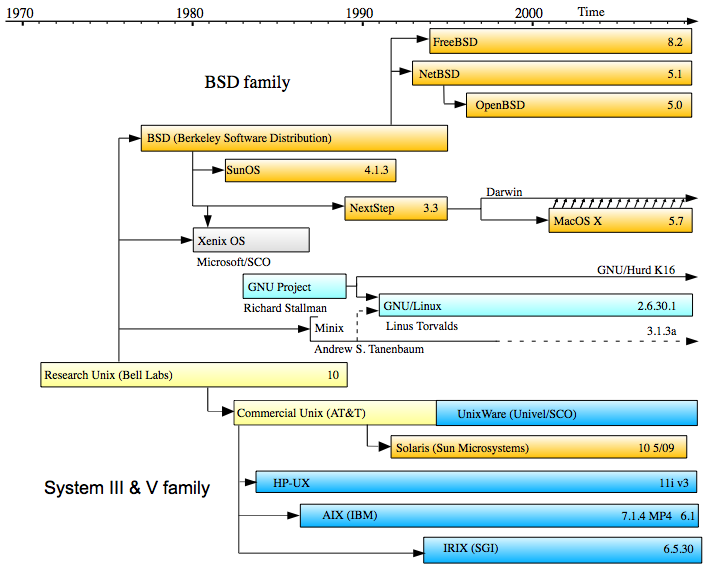
\includegraphics[width=0.75\textwidth]{02/pics/unix_history}
	\caption[Unix genealogy tree]{A partial Unix genealogy tree.
		\label{fig:unix-history}}
\end{figure}

Parallel to the development of the various Unix
flavors evolved a set of standards that helped define
how exactly the operating system should behave, what
interfaces it should provide and what kinds of
assumptions third-party software could make about the
environment.  These standards became to be known as
the ``Single UNIX Specification\index{Single UNIX
Specification}'' (SUS, commonly referred by version,
such as SUSv3) and eventually as
``\glslink{posix}{POSIX}\index{POSIX}'' (for
``Portable Operating System Interface for uniX'').
The SUS was used to qualify operating systems for the
name ``\textsc{UNIX}\index{UNIX}'' -- this
certification was obtained only by a relatively small
number of systems, since it was costly and required
re-certification of the system after any significant
change (i.e., major OS release), something that Open
Source projects, such as the BSDs certainly could not
afford.

Eventually, SUSv3 and POSIX:2001 (formally known as
\glslink{ieee}{IEEE} 1003\index{IEEE 1003}.1-2001)
became more or less interchangable; we will commonly
refer to systems or interfaces as being
``POSIX-compliant'' (or not, as the case may be).  At
the time of this writing, the latest version is
POSIX:2008\cite{history:posix2008}, which is divided
into a {\em Base Definition}, the {\em System
Interfaces and Headers}, and the {\em Commands and
Utilities}.  It should be mentioned, though, that
not only is ``the nice thing about standards that you
have so many to choose
from''\cite{history:tanenbaum-standards}, as an old
phrase coined by Andrew S.
Tanenbaum\index[names]{Tanenbaum, Andrew S.} goes,
but also that a recommendation or requirement does not
necessarily have to make sense or be realistic to be
included in a standard.  We will occasionally notice
discrepancies between what POSIX demands and what
different OS vendors chose to implement.  As two
entertaining examples, please refer to the section of
the \manpage{fcntl(2)} manual page on e.g. a NetBSD
system\cite{history:fcntl} that elaborates on the
locking semantics or the fact that POSIX could be
interpreted to require a \manpage{cd(1)} {\em
executable}\footnote{If the problem of a {\tt cd(1)}
{\em executable} isn't immediately obvious to you...
well, see Problem \ref{prob:cd}!}.

\subsection{Networking}
\label{unix:networking}

No review of the history and basic features of the
Unix operating system would be complete without a
mention of the parallel evolution of the Internet.  As
we noted in Section \ref{unix:history:os}, the
development of the Unix system and that of the
predecessors of what ultimately became the Internet
were not only related, but became inseparably merged.
The ARPANET\index{ARPANET} implemented the concept of
{\em packet switching\index{packet switching}},
allowing payload to be broken into small {\em
datagrams} and routed along different paths; its
adoption of TCP/IP\cite{history:cerf-kahn:tcp} as its
protocol suite effectively marked the beginning of the
modern Internet.  Even though some companies developed
their own TCP/IP stack, the code included in the
Berkeley Software Distribution quickly became the most
widely used implemention and ultimately replaced other
network protocols\footnote{Microsoft, for example, did
not include TCP/IP in their operating systems until
Windows 95, allowing other companies to sell their
implementations as add-on software.  The move from
their native  NetBIOS\index{NetBIOS} protocol to the
BSD derived TCP/IP stack helped make the latter the
de-facto Internet standard protocol suite.}.

In the early days of the Internet, the various
different networks -- ARPANET,
\glslink{csnet}{CSNET}\index{CSNET},
\glslink{milnet}{MILNET}\index{MILNET},
\glslink{nsfnet}{NSFNET}\index{NSFNET},
\glslink{nsi}{NSI}\index{NSI}, etc. -- were connected
via specific gateway hosts, and email exchanges as
well as communications on the early
\glslink{bbs}{BBS}\index{BBS}es and
Usenet\index{Usenet} were performed via
\manpage{UUCP}, the {\em Unix-to-Unix Copy}
tools\footnote{Every now and then you may encounter
a scruffy oldtimer who insists on pointing out that
their email address is something along the lines of
``...!orgserver!deptserv!mybox!user''. You can
trivially impress them by calling it their ``bang
path'' and agreeing that @-based email addresses are
newfangled humbug.}.  Once hosts were more frequently
directly connected to the Internet,
\glslink{smtp}{SMTP}\index{SMTP} and NNTP\index{NNTP}
became more widely used, leading to Unix servers
running various so-called  d\ae mon\index{d\ae mon}s
to provide network services as part of their normal
operations.  \\

But even before the advent of the Internet, Unix
included networking capabilities.  Through its layers
of abstraction it was possible to implement support
for different networking technologies and allow
applications to be network protocol agnostic.  In
fact, some applications, such as  email\index{email}
were available and in use prior to any traditional
networking capabilities.  The nature of Unix as a
multiuser system lead to the development of tools,
amongst them the \manpage{mail(1)} program, to allow
these users to communicate efficiently with one
another and across systems.  We will frequently review
how the nature of a scalable tool allows it to
function equally well regardless of where input data
comes from or what transport mechanism is used; a
simple, well defined program can deliver mail on a
single system while relying on a separate transport
service (i.e., UUCP or SMTP) to handle connections
with other systems.

Furthermore, the software implementing such services
was developed on and then included in the Unix
operating system.  As a result, the Internet and its
infrastructure were growing in parallel to the
capabilities of Unix, one enabling the other to become
more powerful and ubiquitous. And so today, the
overwhelming majority of the systems powering the core
infrastructure components of the Internet, such as,
for example, the \glslink{dns}{DNS} root
servers\index{Domain Name System!root servers} or most
web- and mail servers, are running on a Unix
variant\footnote{As noted in the introduction, we
continue to count Linux as a ``Unix variant'' to avoid
constant repition of the phrase ``Unix or Linux''.}:
the by far most popular implementation of the DNS
specification is, not surprisingly, the {\em
\gls{bind}} server\cite{history:dns-survey};
\manpage{sendmail}, \manpage{exim}, and
\manpage{postfix} push the majority of the world's
email\cite{history:esoft-mx}; the
\manpage{apache}\index{\tt apache} web server
still handles more than 45\% of all
\glslink{http}{HTTP} traffic on active sites than any
other web server\cite{history:netcraft-http}.


\subsection{Open Source}
\label{unix:open-source}

Unix is an inherently open system.  Developed at a
renowned research institution, it was released and
licensed together with the source code long before the
formal idea of ``Open Source\index{Open Source}'' had
manifested itself.  As we have seen in Section
\ref{unix:history}, the availability of the source
code made it possible for other various commercial
versions to be developed by different companies, but
it also allowed the development of the \gls{bsd} with
its distinctly permissive licensing terms.

Having access to the source code of the operating
system and all the tools in use is a foreign concept
in the world of proprietary software, where the source
code is guarded as a trade secret, the pillar upon
which a traditional company builds its entire profit
model.  Within the academic world in which Unix was
developed, however, access to the source code was only
natural.  Peer review and openness were fundamental
parts of this world and the system was targeted
towards engineers, hackers, advanced users who would
naturally like to make changes to tools, who would
want to extend the capabilities and add new features.

This wish to share one's work with others, to allow
others to take full advantage of it, and to make their
own modifications took two distinct directions early
on, embodied in the two open source license models
that have remained dominant to this day.  On the one
hand, the distinctly academic
BSD-License\index{BSD!License} (see Listing
\ref{code:bsdlicense}) allowed for any use of the
software whatsoever (including modification and
commercial re-selling of the products) so long as
credit was given where credit was due.  On the other
hand, the \gls{gpl}\index{GPL}, written by Richard
Stallman\index[names]{Richard Stallman} intended to
very specifically not only {\em grant}, but to {\em
enforce} certain freedoms using a moral argument.
This license, somewhat ironically, imposes a number of
restrictions on what you can do with the source code
you have received, most notably the requirement to
make public under {\em the same} license any changes
you distribute.

People have argued about the benefits of one license
over the other for decades by now, and we will not
attempt to resolve the dispute in this book.  They
represent different approaches to one's software,
perhaps a personal choice of how one wishes that it be
used in the future.  Suffice it to say that there is
incredible software licensed using both approaches,
and both models thrive to this day.  A similar
discussion involves the concept of cost and freedom
with regards to software (``Free as in beer versus
free as in speech'').  Open Source software, like all
software, comes at a price: a relatively small
component of the total cost of ownership is the actual
purchase price, and access to the source code (which
in some cases may well come under specific terms of
the license with commercial and/or closed source
software) is somewhat independent thereof.  What's
more important -- within the context of this book,
anyway -- is that the very concept of Open Source is
embedded in the Unix philosophy and culture, and as a
result System Administrators frequently {\em expect}
to be able to analyze the source code to the
applications and operating systems they run.

But not only are we {\em able} to inspect how a piece
of software works, we {\em need} to.  All too
frequently do we encounter problems or try to analyze
a system's behaviour where the question of what on
earth might be going on is answered with this advice:
``Use the source, Luke!'' -- Unix has let us do
precisely that since the beginning.\footnote{It should
be mentioned that the various commercial Unix versions
represent closed source systems.  But not only are
Open Source Unix versions nowadays much more widely in
use, virtually all of the core software running {\em
on top} of the (commercial, closed, open, or any
other) OS traditionally comes with its source code.}


\section{Basic Unix Concepts and Features}
\label{unix:basics}

The Unix operating system consists, somewhat
simplified, of three major components: a {\em kernel},
which controls the hardware, schedules tasks, and
interfaces with the various devices; a set of {\em
libraries}, which provide an interface to the kernel
(in the form of {\em  system calls\index{system
calls}} that run in privileged kernel space as well as
unprivileged {\em library functions} running in user
space); and a set of {\em tools and applications}
(often referred to as the ``userland'') using these
libraries to provide functionality to the end user.

Most Unix flavors use a {\em
monolithic}\index{kernel!monolithic} kernel, but allow
for dynamically loaded kernel
modules\index{kernel!loadable modules}.\footnote{A
discussion of {\em microkernels}\index{microkernel},
{\em unikernels}\index{unikernel}, and the various
{\em containers} that became popular in more recent
years is, unfortunately, well beyond the scope of this
chapter.  The broad subject matter of System
Administration again forces us to focus on the general
principles first.}    This approach allows for a
reduction of the kernel footprint and increased
flexibility, as device driver support can be added or
removed at runtime without requiring a reboot.  The
kernel, managing the system's resources, is running in
supervisor mode and exposes facilities via system
calls.  It is desirable to keep the number of these
entry points into kernel space limited and let
higher-level library functions provide added
functionality executed in unprivileged mode.
Therefore, most Unix versions have only a
comparatively small number of system calls: as of
January 2017,  NetBSD\index{NetBSD}, for example, had
only around 482 such
calls\cite{history:nbsd-syscalls}, with only minimal
expected growth\footnote{Revisiting an earlier draft
of this chapter from January 2012 listed 472 system
calls.  That is, over the course of five years, only
ten new system calls were added.}.

Utilizing these system calls and library functions,
the higher level tools and applications are able to
interface with the kernel and execute on the user's
behalf.  These binaries then can be divided into a
number of categories, such as executables essential
for the basic operation of the system, tools primarily
intended for use by the system administrator, and
general purpose utilities.  We will revisit this
topic in more detail in Chapter
\ref{chap:software-installation}.

\subsection{The shell}
\label{unix:basics:shell}

The Unix {\em shell}, while in many ways nothing but a
regular executable, takes a special place in the list
of utilities and commands available on the system.
The shell provides the primary user interface,
allowing for the invocation and execution of the other
tools.  AT\&T's Version 7 Unix included the so-called
``Bourne shell''\index{shell!Bourne} (named after
Steven Bourne\index[names]{Bourne, Steven}) installed
as {\tt /bin/sh}.  In addition to the ability to
invoke other commands, the shell was designed as a
{\em command interpreter} both for interactive use as
well as for {\em non}-interactive use.  That is, it
included a scripting language, allowing for complex
series of commands to be executed; for example, by
system startup scripts at boot time.\footnote{It is
worth noting that the early Bourne shell also included
support for pipelines (invented by Douglas McIlroy and
added to Unix by Ken Thompson in 1973).}

\begin{lstlisting}[float,label=code:io-redir,caption=Simple I/O redirection in the shell]
$ cmd >output          # redirection of stdout to a file
$ cmd >/dev/null       # suppression of output
$ cmd >/dev/null 2>&1  # suppression of all output
$ cmd <input           # accepting input from a file
$ cmd1 | cmd2          # feeding output from cmd1 into cmd2

# Of course these redirections can be combined...
$ cmd1 2>/dev/null | cmd2 | cmd3 2>&1 | cmd4 >file 2>output
\end{lstlisting}


Various other shells have been created since then,
mostly following either the general Bourne shell
syntax or that of Bill Joy's\index[names]{Joy, Bill} C
\manpage{csh(1)} Shell.  The most notable shells today
include: the Almquist shell \manpage{ash(1)}, a
BSD-licensed replacement for the Bourne shell,
frequently installed as {\tt /bin/sh} on these
systems; the GNU Project's Bourne-again
shell\index{shell!Bourne-again} \manpage{bash(1)},
which is the default shell on most Linux systems and
known for a large number of added features; the Korn
shell \manpage{ksh(1)}, named after David
Korn\index[names]{Korn, David} and which became the
basis for the POSIX shell standard; the TENEX C shell
\manpage{tcsh(1)}, a C shell variant developed at
Carnegie Mellon University; and perhaps the Z shell
\manpage{zsh(1)} another very feature rich Bourne
shell variant.

As a scripting language and due to its availability on
virtually every Unix flavor, {\tt /bin/sh} is assumed
to be the lowest common denominator: a Bourne- or
Bourne-compatible shell.  On Linux, {\tt bash(1)} is
typically installed as both {\tt /bin/bash} and {\tt
/bin/sh}, and it behaves (somewhat) accordingly based
on how it was invoked.  Unfortunately, though, its
ubiquity on Linux systems has led to a shell scripts
masquerading as {\tt /bin/sh} compatible scripts that
are, in fact, making use of {\tt bash(1)} extensions
or rely on {\tt bash(1)} compatibility and syntax.
This becomes frustrating to debug when trying to run
such scripts on a platform with a POSIX compliant {\tt
/bin/sh}.  \\

All Unix shells include the ability to perform  I/O
redirection\index{I/O redirection}.  Each program has
a set of input and output channels that allow it to
communicate with other programs.  Like the concept of
the pipe, these streams have been part of Unix's
design from early on and contribute significantly to
the consistent user interface provided by all standard
tools:  a program accepts input from {\em standard
input} (or \manpage{stdin}) and generates output on
{\em standard output} (or \manpage{stdout}); error
messages are printed to a separate stream, {\em
standard error} (or \manpage{stderr}).

The shell allows the user to change what these streams
are connected to; the most trivial redirections are
the collection of output in a file, the suppression of
output, acceptance of input from a file, and of course
the connection of one program's output stream to
another program's input stream via a pipe (see
Listing \ref{code:io-redir} for Bourne-shell
compatible examples).

The concept of these simple data streams being
provided by the operating system was inherent in the
Unix philosophy\index{Unix!Philosophy}: it provided
abstraction of interfaces, reduced overall complexity
of all tools using these interfaces, and dictated a
simple text stream as the preferred means of
communication.  We will have more to say on the Unix
philosophy in Section \ref{unix:philosophy}.

\begin{figure}[t]
	\centering
	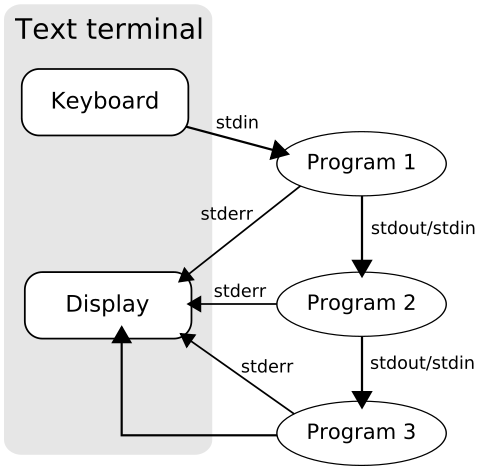
\includegraphics[width=0.5\textwidth]{02/pics/pipeline}
	\caption{Standard streams in a simple pipeline
		\label{fig:streams-pipeline}}
\end{figure}


Finally, the unix shell provides for {\em  job
control}\index{job control}, a necessity for a
multitasking operating system.  When a user logs into
the system, their {\em  login shell}\index{login
shell} is started, serving as the primary interface
between the user and the OS.  After entering a command
or a pipeline, the shell will create (``fork'') a new
process and then execute the given programs.  The
standard streams are connected as illustrated in
Figure \ref{fig:streams-pipeline}.  While the program
or pipeline is running, the user cannot do anything
else -- she has to wait until the command completes
and control is returned to the shell.  In the mean
time, all she can do is twiddle her thumbs; so much
for multitasking!

\begin{lstlisting}[float,label=code:sh-jobcontrol,caption=Simple job control in the shell]
$ cmd1 &            # send cmd1 to the background
[1] 5836            # report job number and process ID
$ cmd2 | cmd3 &     # send a process group to the background
[2] 5912
$ jobs              # report on running jobs
[1]  Running    cmd1
[2]  Running    cmd2 | cmd3
$ fg %1             # bring job 1 to the foreground
cmd1
^Z                  # suspend via Control+Z
[1]+ Stopped    cmd1
$ bg                # send it back to the background
[1]+ cmd1
$                   # hit return again...
[1]+ Done       cmd1
$                   # cmd1 has completed
\end{lstlisting}

To avoid this scenario, the C shell implemented a
feature that was quickly incorporated in the Bourne
shell, which allows users to start and control
multiple concurrent processes by placing them into the
{\em background} (by adding the {\tt \&} symbol at the
end of the command or via the shell {\tt builtin}s),
bringing them to the {\em foreground} (via {\tt
builtin}s), suspending and continuing them (by sending
possibly keyboard generated signals to the relevant
process group), etc.  Listing \ref{code:sh-jobcontrol}
illustrates the basic job control functionality.

\subsection{Manual pages and documentation}
\label{unix:basics:manual}

Another important feature of the Unix operating system
was that it included what came to be known as the
``online manual pages''\index{Manual
Pages}\footnote{In Unix's historic context,
``online'' initially meant that the documentation is
available on the running system, not ``on the
Internet''.}, reference documentation readily
available on the running system and that went beyond
just attesting to the existence of a command or
feature, but instead provided actually useful
information, including the correct invocation,
possible options, a description of the tool's
functionality as well as any known bugs.  Divided into
several sections by topic,  system calls are
documented in section two, library functions in
section three, while commands and executables are
usually documented in section one for general purpose
tools and section eight (on BSD, section {\tt 1M} on
SysV derived systems) for system administration
related commands and d\ae mons.

The standard for this documentation has always been
high, reflecting the academic culture behind the
operating system.  Rather than treat the user as a
naive consumer, Unix documentation acknowledges the
fact that the target audience consists of skilled
engineers who appreciate and require an accurate
description of the tools at their disposal in order to
make the most of them.  It may not surprise you to
know that the adoption of Unix within the Bell
Labs\index{Bell Laboratories} patent office, which
secured funding for further development, was largely
thanks to the system's abilities to typeset beautiful
documents using the {\em roff} text formatting
program\footnote{Consider that W. Richard
Stevens\index[names]{Stevens, W.  Richard} used to
typeset his famous books ``Advanced Programming in the
UNIX Environment'' and the ``TCP/IP Illustrated''
series by himself using {\tt groff(1)}.}.  The same
tools are still used to format the manual pages.

Unix provided manual pages and documentation not just
of the executables and configuration files provided by
the system, but also for so-called ``supplementary''
documents.  These comprise a number of papers that,
as in the case of the \gls{ipc}\index{IPC} tutorials,
for example, served as the de-facto reference
documentation and continue to be used in countless
Computer Science classes today to teach students the
fundamentals of Unix IPC.  Other highlights include an
introduction to the GNU debugger {\tt gdb}, the {\tt
make} tool, a \manpage{vi(1)} reference manual, an
overview of the file system, and various d\ae mons.
Since these documents are licensed under the
permissive  BSD License\index{BSD!License}, they can
be -- and thankfully are! -- included in modern Unix
versions (such as e.g. NetBSD\index{NetBSD}) and made
available on the Internet\cite{history:nbsd-docs}.

\begin{sidenote}
{\bf Understanding the Shell} \\
A System Administrator spends a significant amount of
time in the shell, both her own login shell as well as
various others.  Not only does she need to run
countless commands to remotely administrate various
hosts, she also routinely writes small, large,
complex, simple, elegant or convoluted scripts to
accomplish any thinkable task.  It is therefore
imperative to understand how the Unix shell works on a
detailed level.  It is surprising how frequently the
many intricacies of I/O redirection, of job control
and pipelines, of aliases and {\tt builtin}s taking
precedence over commands, as well as other seemingly
obscure problems manifest themselves. \\ [10pt]

If you have a background in C programming, consider
writing a general purpose Unix shell from scratch --
it will teach you invaluable lessons about how the
system works on a very fundamental level.  (If you do
not have a background in C programming... develop
one!)
\end{sidenote}



\subsection{A portable, multitasking, multiuser system}
\label{unix:basics:multi}

The Unix operating system was, from the very
beginning, designed as a {\em portable}, {\em
multitasking}, {\em multiuser} system.  These inherent
features are largely responsible for the incredible
success of this over 40 year old system and each has
wide-reaching consequences.  Initially developed on a
PDP-7\index{PDP-7} and then a PDP-11\index{PDP-11}
machine, Unix was rewritten in the C\index{C}
programming language, which allowed it to be ported
with comparatively little effort to various other
machines and hardware architectures. Figure
\ref{fig:portability} shows a few different hardware
platforms, each running a version of Unix.  Prior to
this, operating systems were written in assembly, and
that was that -- only a fool would attempt otherwise!
But as a result of this bold move to stray from
convention and instead to apply a fundamental design
choice of abstraction of complexity, the system became
inherently portable: software {\em for} Unix -- any
Unix, really -- can usually be adapted to other Unix
flavors with few modifications.

\begin{figure}[t]
	\centering
	\begin{minipage}{.4\linewidth}
		\centering
		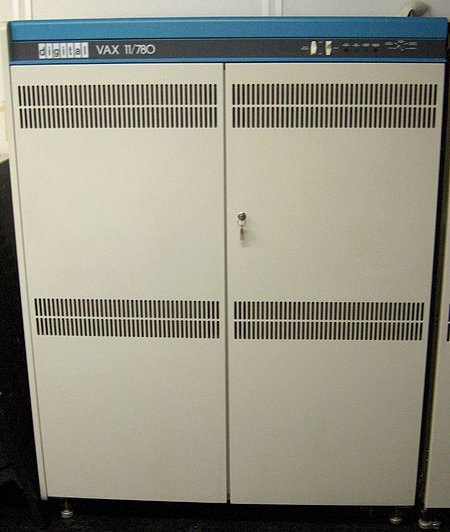
\includegraphics[width=0.9\textwidth]{02/pics/VAX_11-780_intero}
	\end{minipage}
	\hfill
	\begin{minipage}{.4\linewidth}
		\centering
		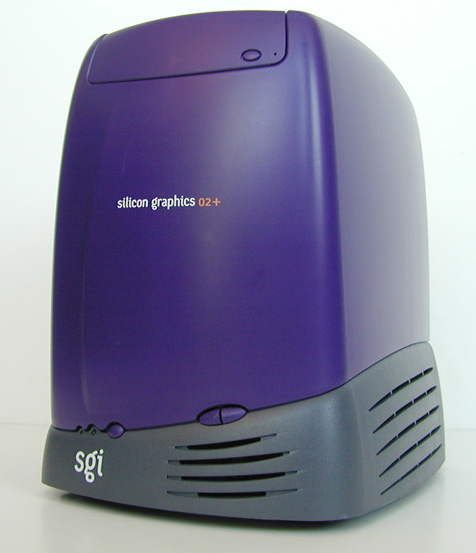
\includegraphics[width=0.9\textwidth]{02/pics/Silicon_Graphics_O2_Plus}
	\end{minipage}
	\\
	\begin{minipage}{.4\linewidth}
		\centering
		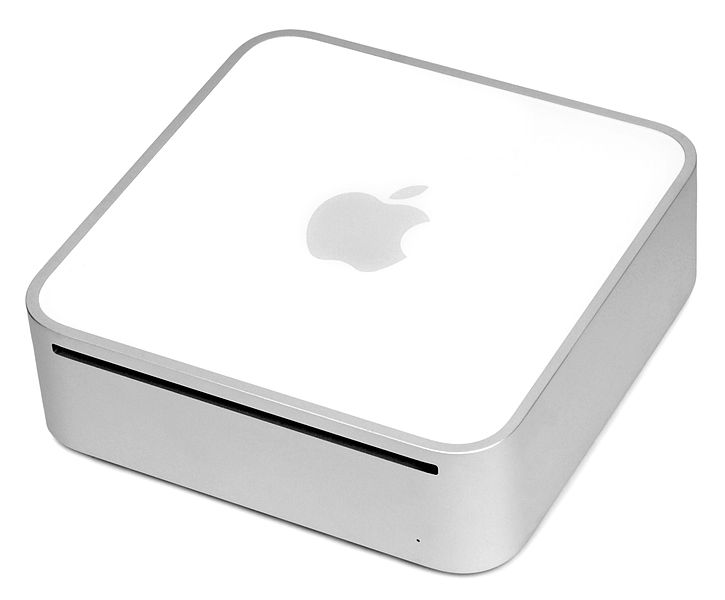
\includegraphics[width=0.9\textwidth]{02/pics/Mac-mini-1st-gen}
	\end{minipage}
	\hfill
	\begin{minipage}{.4\linewidth}
		\centering
		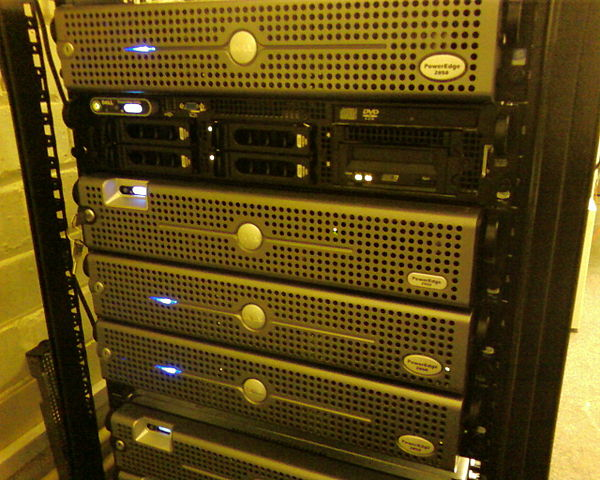
\includegraphics[width=0.9\textwidth]{02/pics/Dellpoweredge2950}
	\end{minipage}
	\caption[Different systems running Unix]{
			Different systems and architectures running Unix.
			A VAX-11 by DEC (VAX), an O2 by SGI (MIPS),
			a Mac Mini by Apple (PowerPC), PowerEdge
			servers by Dell (x86).
				\label{fig:portability}}
\end{figure}


Now, to state that Unix is {\em portable} does not
mean that one can trivially recompile the software
without any changes -- far from it!  Any System
Administrator can relate stories of having spent
hours wrangling Makefile\index{Makefile}s, {\tt
autoconf}/{\tt automake}\index{\tt autoconf}\index{\tt
automake} frameworks, and hunting down header files
and libraries.  But in the end, it remains
relatively easy to get the software to work, since all
Unix systems follow (to some degree, anyway) certain
standards and conventions.  Consider the effort of
adapting a complex piece of software from running on
Linux to, say, IRIX\index{IRIX} to that from running
on Windows 95 to Mac OS 9!  Unix having been rewritten
in the higher level C programming language, the
standardization of C, as well as the POSIX guidelines
really allowed a world of portable, flexible software
to flourish.

The {\em multitasking} nature of the Unix operating
system was a given, as it was intended to be a
time-sharing system, allowing multiple processes to
use the given resources seemingly simultaneously by
means of a scheduler which initiates context switches
to grant each process time on the
\gls{cpu}\index{CPU}.  Allowing for multiple
(simultaneous) users was just a logical consequence.
Nowadays it may not seem worth mentioning, but it is
worth noting that this system, conceived to allow
multiple users simultaneous access was designed over
40 years ago.  In comparison, Windows NT\index{Windows
NT}, first released in 1993, was the first of
Microsoft's family of operating systems to eventually
introduce multiuser capabilities, around 20 years
later; Apple\index{Apple}'s Mac OS gained multiuser
capabilities only with OS X\index{OS X} in 2001.

The nature of a {\em multiuser} system has a number of
significant implications:  A system that allows
multiple users to simultaneously utilize the given
resources is in need of a security model that allows
for a distinction of access levels or privileges.  The
system needs to be able to distinguish between file
access or resource utilization amongst users, thus
requiring the concept of access permissions, process
and file ownership, process priorities and the like.
Controlling access to shared resources by individual
users also required, effectively, a single omnipotent
user to control and administer these privileges, thus
necessitating the superuser or {\tt root
account\index{root account}} (with plenty of security
implications and concerns of its own).

In order to meet these requirements, the Unix system
uses a set of file permissions to restrict three
different types of access -- read, write and execute
(or {\tt rwx}, respectively) -- to the file {\em
owner} or {\em user}, members of a specific user {\em
group}, or everybody else (i.e., {\em others}) on the
system ({\tt ugo}, respectively).  These permissions
can be used to implement efficiently various security
models, but at the same time they are simple and
flexible enough to allow users to make their own
choices.\footnote{Different Unix versions have since
developed support for extended file
attributes\index{File Systems!Extended attributes}
including e.g. a per-file \gls{acl}\index{Access
Control Lists}, allowing the user
to wield more fine-grained control.  This is
implemented on different operating systems and in
different file systems, and the details and semantics
differ. In the interest of simplification and focusing
on the fundamental principles, we are not covering
\gls{acl}s.}

Unix has a long tradition of following the {\em
principle of least privilege}\index{Security!Principle
of Least Authority}: system services are usually run
using a dedicated user account, allowing the System
Administrator to separate file access and resource
usage such that even if the service was compromised,
harm would be minimized.  This practice translates
to routine tasks in system administration and standard
operating procedures alike.  We will revisit this
concept in more detail in Chapter \ref{chap:security}.

Processes, like files, are associated with individual
users, though privilege escalation\index{privilege
escalation} can be accomplished by means of changing
the {\em effective user ID}\index{EUID}\index{\tt
setuid(2)}.  Processes also may have specific resource
limitations, which the superuser can set system-wide
or on a per-user or per-group basis.  We will revisit
the associated system calls and commands like
\manpage{getrlimit(2)}, \manpage{sysctl(8)},
\manpage{ulimit(1)}, and {\em login
classes}\index{login classes} (see
\manpage{login.conf(5)}, where available) in Chapter
\ref{chap:monitoring} and elsewhere.

\subsection{The Unix Philosophy}
\label{unix:philosophy}

The design of the Unix operating system was based on
principles that not only have been proven time and
again to lead to stable, scalable and robust
solutions, but that have formed the basis of a
specific Unix culture\index{Unix!culture}, a way of doing things that
speaks to advanced users such as System Administrators
in particular.  You can find a thorough explanation of
this culture in classic texts such as
Kernighan\index[names]{Kernighan, Brian W.} and
Pike's\index[names]{Pike, Rob} ``The UNIX Programming
Environment''\cite{history:kernighan-pike-upe}, Eric
S.  Raymond's\index[names]{Raymond, Eric S.} ``The Art of Unix
Programming''\cite{history:esr-taoup}, or simply by
searching the Internet for the term ``Unix
philosophy'', but it warrants summarizing due to the
profound impact it has.

At its core, the  Unix
philosophy\index{Unix!Philosophy} stipulates that
tools should be kept simple and adhere to specific
simple guidelines and implement an equally simple
interface (namely text streams).  Virtually every one
of the great minds involved in the initial invention
and continued development of the Unix operating
system -- from Douglas McIlroy\index[names]{McIlroy,
Douglas} to Rob Pike\index[names]{Pike, Rob}, from
Dennis Ritchie to Ken Thompson -- can be quoted to
underline this point; they must have been on to
something.

The most well-known expression of what makes Unix Unix
is probably Douglas McIlroy's\index[names]{McIlroy,
Douglas}
summary\cite{history:mcilroy-unix-philosophy},
partially cited in the previous chapter:

\begin{quote}
{\em Write programs that do one thing and do it well. Write programs to work
together. Write programs to handle text streams, because that is a
universal interface.}
\end{quote}

This is frequently succinctly described as the KISS
(``Keep it simple, stupid'') principle and correlated
with Richard P. Gabriel's\index[names]{Gabriel,
Richard P.} ``Worse is Better\index{Worse is
Better}''\cite{history:gabriel-worse-is-better} design
philosophy, according to which simplicity is to be
preferred over all other attributes of software, at
times even including correctness.  While I do not tire
of repeating precisely this advice, I believe that the
existing literature tends to overlook, one major
factor that helped arrive at the mantra of simplicity:
deference to the user.

One of the smartest insights a program or system
developer can have is that even though they are the
person writing the software, they cannot foresee all
possible uses of the software.  They cannot know what
the user will want to accomplish or in what ways she
may wish to use the tool.  And therein lies the crux:
if I wish to enable the user to utilize the tool in
any way they wish, how can I possibly keep it simple?
Wouldn't it have to end up being a general purpose
tool, with countless inherent complexities as I
attempt to anticipate every interface of the future?
Remember, a ``general purpose product is harder to
design well than a special-purpose
one.''\cite{history:brooks-design}

This is where the Unix philosophy comes in: by
imposing restrictions, it counterintuitively opens up
the most flexible, the widest use.  Simple tools that
perform a single task and operate on a well-defined
interface are less complex than software that attempts
to keep state in deeply nested data structures (or,
worse yet: binary objects stored in files).  Our users
gain the ability to use the tools for purposes we did
not initially anticipate.  Unix grants the user
flexibility.  For  better or worse, Unix trusts its
users to know what they're doing and will happily let
you shoot yourself in the foot.

\begin{quote}
{\em \textsc{UNIX}\index{UNIX} was not designed to
stop its users from doing stupid things, as that would
also stop them from doing clever things.} -- Doug
Gwyn\index[names]{Gwyn, Doug}
\end{quote}



The awareness that your software might be used in ways
you cannot imagine, that the user of the software
might actually know better what they may wish to
accomplish than the designer or implementer is what
makes Unix so fascinating.  Interestingly, this
philosophy, this trust into the user and his or her
capabilities and knowledge stands in stark contrast
to that of the late Steve Jobs\index[names]{Jobs,
Steve}, who famously quipped that ``people don't know
what they want until you show it to
them''\cite{history:jobs}.  Apple's products are known
for their elegance and ease of use, but advanced users
know that should you attempt to do something with them
that the designers did not anticipate, it's either
impossible or painfully cumbersome.

The primary user interface on the Unix systems remains
the command-line\glslink{cli}.  This is not for a lack
of other options, but a manifestation of the Unix
philosophy.  While it may appear more
``user-friendly'' to a novice to use a pointing device
to select pre-determined options from a menu using a
\gls{gui}, it is anathema to efficient System
Administration.

System Administrators need to be able to perform tasks
remotely, quickly, and reliably unattended; execution
of programs needs to be automated and scheduled,
configuration be done outside of the application, and
data be transformed with the myriad of available
filters.  As you can tell, these requirements go back
to the Unix way of writing simple tools that work well
together by communicating via text streams.
Thanks to the consistency with which these principles
are implemented across the platform, the learning
curve for advanced users, while perhaps steeper than
on some other systems, only needs to be climbed
once.  At the same time, it gets you to a higher level
of efficiency quickly.  \\

The ability to combine individual tools to build
larger, more complex ones; to remotely access hundreds
or thousands of systems in the same manner as one
would a single system; to allow rapid development of
simple prototypes constructed of growing pipelines; to
be able to control access to shared resources
following a simple yet flexible security model; to
extend and tune the operating system itself; to be
able to do all the things that the designers of the
system could not have envisioned you doing -- this
power is what Unix confers upon the advanced user.  It
is why System Administrators not only prefer Unix, but
actually enjoy working on this platform.

\begin{lstlisting}[float,label=code:bsdlicense,caption={[2-clause
BSD license]The simplified, or 2-clause, BSD license.
Nice and terse, huh?  In contrast, the \gls{gnu}
\gls{gpl} clocks in at 11 full text pages.}] 
Copyright (c) <year>, <copyright holder>
All rights reserved.

Redistribution and use in source and binary forms, with or
without modification, are permitted provided that the
following conditions are met:

1. Redistributions of source code must retain the above
   copyright notice, this list of conditions and the
   following disclaimer.
2. Redistributions in binary form must reproduce the
   above copyright notice, this list of conditions and
   the following disclaimer in the documentation and/or
   other materials provided with the distribution.

THIS SOFTWARE IS PROVIDED BY THE COPYRIGHT HOLDERS AND
CONTRIBUTORS "AS IS" AND ANY EXPRESS OR IMPLIED
WARRANTIES, INCLUDING, BUT NOT LIMITED TO, THE IMPLIED
WARRANTIES OF MERCHANTABILITY AND FITNESS FOR A PARTICULAR
PURPOSE ARE DISCLAIMED. IN NO EVENT SHALL THE COPYRIGHT
OWNER OR CONTRIBUTORS BE LIABLE FOR ANY DIRECT, INDIRECT,
INCIDENTAL, SPECIAL, EXEMPLARY, OR CONSEQUENTIAL DAMAGES
(INCLUDING, BUT NOT LIMITED TO, PROCUREMENT OF SUBSTITUTE
GOODS OR SERVICES; LOSS OF USE, DATA, OR PROFITS; OR
BUSINESS INTERRUPTION) HOWEVER CAUSED AND ON ANY THEORY
OF LIABILITY, WHETHER IN CONTRACT, STRICT LIABILITY, OR
TORT (INCLUDING NEGLIGENCE OR OTHERWISE) ARISING IN ANY
WAY OUT OF THE USE OF THIS SOFTWARE, EVEN IF ADVISED OF
THE POSSIBILITY OF SUCH DAMAGE.

The views and conclusions contained in the software and
documentation are those of the authors and should not be
interpreted as representing official policies, either
expressed or implied, of <the project>.
\end{lstlisting}

\pagebreak

\chapter*{Problems and Exercises}
\addcontentsline{toc}{chapter}{Problems and Exercises}
\section*{Problems}

\begin{enumerate}
\item
Research the history of the Unix operating system in more detail.  Branch
out into the ``USL vs. BSDi'' lawsuit.  Follow the BSD genealogy into the
Mac OS X system.  Analyze the future direction of the commercial Unix
versions.

\item
Review the Linux, NetBSD and Solaris versioning numbers.  Try to correlate
specific features to specific releases across these systems (note the
different Linux distributions numbers as well).

\item
Review the {\tt intro(1)} manual pages on your system (they may exist for
different sections and, depending on the Unix flavor, in varying detail).
From there, move on to the following manual pages, considering the
multiuser implications: {\tt chmod(1)}/{\tt chown(1)}, {\tt login(1)},
{\tt passwd(5)}, {\tt su(1)}, {\tt sudo(8)}

\item
\label{prob:cd}
Does the POSIX standard really require a {\tt cd(1)} {\em executable}?  If
it did, what might be a problem with that?  Consider the environment of a
process and how a shell executes commands.

\item
Play around in the Unix environment of your choice.  Look at the
executables found in the system's path ({\tt /bin}, {\tt /usr/bin}, {\tt
/sbin}, {\tt /usr/sbin}) -- do you know what all these tools do?

\item
Review your understanding of the Unix philosophy of simple tools acting as
filters.  Does this reflect your usage of the tools you most frequently
execute?  Which tools do {\em not} work (well) as a filter?  Why?

\item
Research the design decisions underlying other popular operating systems.
In how far do they differ from those presented here?  Do they influence or
reflect the primary user base (i.e., what is cause and what is effect)?  How
do they affect or relate to System Administration, especially on a large
scale?

\end{enumerate}

\section*{Exercises}
\addcontentsline{toc}{section}{Exercises}

\begin{enumerate}
\item
Using the programming language of your choice, write a simple interactive
shell capable of executing programs on the user's behalf.  Try to use it
as your shell.  Were you aware of the limitations before you did this?
Were you aware of the complexity of even basic features?

\begin{enumerate}

\item
Compare your shell to some of the existing implementations.  What features
are missing from your shell?  How difficult do you think would it be to
implement them?

\item
Add additional features to your shell, such as support for input/output
redirection, pipelines, expansion of environment variables or job control.
(Note: this is a {\em significant} project, but you will learn a great
deal about the Unix operating system in the process.)

\item
Research and review the concept of a {\em restricted shell}.  Would
writing such a shell be {\em more} or {\em less} effort to do?
\end{enumerate}

\end{enumerate}

\pagebreak

\bibliographystyle{plainnat}
\begin{thebibliography}{99}

\bibitem{history:top500} TOP500; on the Internet at
\url{https://www.top500.org/statistics/list/}
(visited January 16, 2017)

\bibitem{history:bell-labs-unix-history}{\em The Creation of the UNIX Operating
System}, on the Internet at
\url{http://www.bell-labs.com/history/unix/}
(visited January 7, 2012)

\bibitem{history:dmr-history}Dennis M. Ritchie, 'The Evolution of the Unix
Time-sharing System', published in {\em AT\&T Bell Laboratories Technical
Journal}, ``Computing Science and Systems: The UNIX System,'' 63 No. 6
Part 2, October 1984;  also available via the Internet Archive at e.g.
\url{https://web.archive.org/web/20150408054606/http://cm.bell-labs.com/cm/cs/who/dmr/hist.html} (visited January 17, 2017)

\bibitem{history:kernighan-pike-upe}Brian W. Kernighan, Rob Pike, {\em The UNIX
Programming Environment}, Prentice Hall, 1984

\bibitem{history:esr-taoup}Eric Steven Raymond, {\em The Art of Unix Programming},
Addison-Wesley Professional, September 2003; also available on the
Internet at
\url{http://catb.org/~esr/writings/taoup/} (visited January 7, 2012)

\bibitem{history:tuhsml}The Unix Heritage Society Mailing List,
\url{http://minnie.tuhs.org/mailman/listinfo/tuhs}

\bibitem{history:adams-h2g2}Douglas Adams, {\em The Hitchhiker's Guide to the Galaxy},
Pan Books, 1979

\bibitem{history:kr}Brian W. Kernighan, Dennis M. Ritchie, {\em The C Programming
Language}, Prentice Hall, 1988

\bibitem{history:dmr-pipes}Dennis M. Ritchie, 'Advice
from Doug Mcilroy'; now only found on the Internet
Archive at
\url{https://web.archive.org/web/20150205024833/http://cm.bell-labs.com/cm/cs/who/dmr/mdmpipe.html}

\bibitem{history:mcilroy-reader}Douglas McIlroy, {\em
A Research UNIX Reader: Annotated Excerpts from the
Programmer's Manual, 1971-1986}; on the Internet at
\url{http://www.cs.dartmouth.edu/~doug/reader.pdf}

\bibitem{history:bsdisuit}'USL vs. BSDI documents', only available on the Internet Archive via e.g.
\url{https://web.archive.org/web/20150205025251/http://cm.bell-labs.com/cm/cs/who/dmr/bsdi/bsdisuit.html} (visited January
18, 2017)

\bibitem{history:torvalds-announce}'What would you like to see most in minix?',
Linus Torvalds, posting to the \url{comp.os.minix} newsgroup on Usenet, on
the Internet at
\url{https://groups.google.com/group/comp.os.minix/msg/b813d52cbc5a044b}
(visited January 16, 2012)

\bibitem{history:bsd-license}{\em BSD Licenses} on
Wikipedia at
\url{https://en.wikipedia.org/wiki/BSD\_licenses} (visited
January 18, 2017)

\bibitem{history:levenez-history}\'{E}ric L\'{e}v\'{e}nez, {\em Unix History}, on
the Internet at
\url{http://www.levenez.com/unix/} (visited January 5,
2012)

\bibitem{history:posix2008}The IEEE and The Open Group, ``The Open Group Base
Specifications Issue 7, IEEE Std 1003.1, 2016 Edition'' on the Internet at
\url{http://pubs.opengroup.org/onlinepubs/9699919799/} (visited January 17,
2017)

\bibitem{history:tanenbaum-standards}Andrew S. Tanenbaum, in 'Computer Networks',
Prentice Hall, 2004

\bibitem{history:fcntl}\manpage{fcntl(2)}, NetBSD
System Calls Manual, on the Internet at
\url{http://netbsd.gw.com/cgi-bin/man-cgi?fcntl++NetBSD-current}
(visited January 18, 2017)

\bibitem{history:nbsd-syscalls}NetBSD system call name/number ``master'' file, on
the Internet at
\url{http://cvsweb.netbsd.org/bsdweb.cgi/src/sys/kern/syscalls.master?rev=HEAD}
(visited January 18, 2017)

\bibitem{history:nbsd-docs}4.4 Berkeley Software Distribution Documentation, on
the Internet at
\url{http://www.netbsd.org/docs/bsd/lite2/} (visited
January 28, 2012)

\bibitem{history:cerf-kahn:tcp}Vinton G. Cerf, Robert E. Kahn, ``A Protocol for
Packet Network Intercommunication'', IEEE Transactions on Communications 22 (5);
also available on the Internet at
\url{http://ece.ut.ac.ir/Classpages/F84/PrincipleofNetworkDesign/Papers/CK74.pdf}
(visited January 28, 2012)

\bibitem{history:dns-survey}DNS server survey, 2004; on the Internet at
\url{http://mydns.bboy.net/survey/} (visited February 4, 2012)

\bibitem{history:esoft-mx}Mail (MX) Server Survey, August 1st, 2007, showed over
60\% of SMTP traffic to originate from a Sendmail, Exim, or Postfix
installation; on the Internet at
\url{http://www.securityspace.com/s\_survey/data/man.200707/mxsurvey.html}
(visited February 4, 2012)

\bibitem{history:netcraft-http}January 2017 Web Server Survey, on the Internet at
\url{https://news.netcraft.com/archives/2017/01/12/january-2017-web-server-survey.html}
(visited January 18, 2017)

\bibitem{history:mcilroy-unix-philosophy}M. D. McIlroy, E. N. Pinson, and B. A.
Tague {\em Unix Time-Sharing System Forward}, The Bell System Technical
Journal. Bell Laboratories, 1978

\bibitem{history:gabriel-worse-is-better}Richard P. Gabriel, ``Worse is Better'',
on the Internet at
\url{http://dreamsongs.com/RiseOfWorseIsBetter.html.html} (visited February 5,
2012)

\bibitem{history:brooks-design}Frederick P. Brooks, Jr., {\em The Design of
Design}, Addison-Wesley Professional, 2010

\bibitem{history:jobs}Steven P. Jobs, as quoted in BusinessWeek (25 May 1998)

\bibitem{history:salus-history}Peter H. Salus, {\em A Quarter Century of UNIX},
Addison-Wesley Professional, 1994

\bibitem{history:tuhs}The Unix Heritage Society, {\em The Unix Archive},
on the Internet at
\url{http://www.tuhs.org/Archive/README} (visited April 11, 2012)

\end{thebibliography}

\chapter{Documentation Techniques}
\label{chap:documentation}

\begin{quote}
{\em Lack of documentation is becoming a problem for acceptance.}
-- Wietse Venema\index[names]{Venema, Wietse}
\end{quote}

\begin{figure}[hb]
	\raggedleft
	
\includegraphics[width=.15\textwidth]{03/pics/pen}
	\label{fig:pen}
\end{figure}

%\begin{figure}[b]
%	\captionsetup{justification=justified,singlelinecheck=false}
%	\caption[A pen]{Mightier than the sword...
%		\label{fig:pen}}
%\end{figure}

We noted in Chapter \ref{unix:basics:manual} that one
of the many ways in which the Unix operating system
distinguished itself from other systems was that it
included extensive documentation of high quality.
Each tool provided by the OS came with a {\em manual
page}\index{Manual Pages} describing its use, each
library included a description of its interfaces, and
configuration files were accompanied by documentation
elaborating on its syntax and format.

Even simple systems cannot be operated, maintained,
updated -- or in a word, administered -- without an
abstract description of the various moving parts.

But while every System Administrator values good
documentation, and will happily agree that, yes, all
systems should in fact be properly documented,
runbooks created, procedures described, and additional
information referenced, it does take practice and
conscious dedication to develop a habit of writing
high quality system documentation\index{system
documentation}.

For this reason, and before we dive into the
fundamental technologies and concepts in Part
\ref{part:fundamentals}, let us briefly focus on a few
principles that help us provide better documentation
due to a better understanding of what purpose it
serves.

\section{System Documentation Writing 101}
\label{documentation:system-documentation-writing}

Writing is communication.  You wish to provide
information for your organization, your users, or
colleagues.  As a reader of system documentation, you
are in search of information.  This exchange of
knowledge is direct communication between the author
of the documents and the reader.

The motivation, purpose, and effective techniques
used in any kind of writing are similar, so allow us
to begin with some advice that, while it may sound like
it was cribbed from a ``Creative Writing 101''
syllabus, still remains sound.

\subsection{Know Your Audience}
\label{documentation:creative:audience}

Understanding who may be reading our documentation is
essential to providing the right information, just as
a software engineer must understand who the product's
users will be.

Knowing your audience means that you understand what
information they are looking for, what background
knowledge they may have, what additional documentation
or resources they may have access to, and so on.

When we create system documentation, we usually target
the following readers\footnote{You will note that this
same advice for ``knowing your audience'' translates
near verbatim to knowing your {\em users} when writing
software.  We will revisit this concept in chapter
\ref{chap:building-scalable-tools}.}: \\

{\em We write documentation for ourselves.} This is
the simplest case, as we know our target audience well
-- or so we think!  For the most part, we are writing
things down so we can repeat them later on, so we
don't forget, so we have a point of reference in the
future.  This means that we have a pretty good idea
what the prospective reader might expect to find, what
they might know about the infrastructure etc.

{\em We write documentation for other system
administrators.} This case is still fairly straight
forward.  We expect our target audience to be very
technical and have a very good understanding of our
systems.  For example, we write down the steps of a
procedure that our colleagues may not normally
perform, or we document the setup of a system
component we are in charge of that is crucial to the
overall operations of our organizations so that they
may use this document as a reference when we are not
available.

{\em We write documentation for other technical
people.} Our services are used by a number of people
in our organization.  Some of these are very technical
expert users, software developers or other engineers,
perhaps.  In order to allow these people to get
information about our systems quickly, we provide
end-user documentation which allows more efficient use
of the resources we make available.

{\em We write documentation for our users.} The
systems we maintain provide a certain service and thus
has users, some of whom may be internal to our
organization and others which may be outside
customers.  It is not rare that the people in charge
of maintaining the systems provide documentation to
these end-users in one way or another to allow them to
utilize the service or help them find help when things
break down.

{\em We write documentation for other people
everywhere.} System administrators rely on the
Internet at large to find answers to the rather odd
questions they come up with in the course of their
normal work day.  Frequently we encounter problems
and, more importantly, find solutions to such problems
that are of interest to other people, and so we strive
to share our findings, our analyses, and our answers.

Some of the most interesting technical blogs are
written by system administrators or operational teams
and describe how they scale their infrastructure to
meet their demands.  Likewise, system administrators
present their findings and solutions at industry
conferences, write technical papers or participate in
Internet standards development, all of which require
expert documentation and writing skills.  \\

The differences in target audience have a certain
impact on how you would structure your documentation
as well as, in some cases, implications on access
control of the information in question.  Internal
documentation targeted towards your peers may well
include certain privileged information that you would
rather not have made available to the entire
organization (or outsiders via the Internet).

As much as the target audience differs, though, the
best advice for writing good technical documentation
is to avoid making any assumptions about the reader's
prior knowledge and familiarity with the systems in
questions.  At the same time, we need to carefully
identify and reference whatever assumptions,
unavoidable and necessary as they may be, {\em are}
being made.

Secondly, it is important to clearly distinguish {\em
internal} from {\em external} documentation.  The
distinction here is not so much between your corporate
or legal identity and the public at large -- an easy
and obvious one to draw and enforce -- but between
distinct entities within a single organization.
Documentation containing certain details regarding
your infrastructure's network architecture, access
control lists, location of credentials and the like
may simply not be suitable to be made available
outside your department.  Unfortunately the boundaries
can be less than obvious as people move in and out of
departments as an organization evolves.

\section{Online Documentation}
\label{documentation:online-documentation}

One of the main differences from creative writing is
that our documentation is in almost all cases intended
to be read online.  Even though certain documents such
as a contact information registry of the support staff
or the emergency escalation procedures may be useful
to have in print, virtually all information we collect
and make available are read in an online or computer
context.  This has a profound impact on the structure
and style of our documents.

Studies (\cite{doc:online-literacy},
\cite{doc:nielson-web-writing}, et al.) have shown
that not all ``reading'' is equal:  content consumed
via a web browser, for example, is frequently only
glanced through, skimmed over or otherwise not paid
full attention to.  When we read documents online, we
tend to search for very specific information; we
attempt to extract the ``important'' parts quickly and
tend to ignore the rest.

As a result, online documentation needs to be much
more succinct than information intended for actual
print.\footnote{Imagine reading this book entirely
online, perhaps as a series of blog posts.  You would
likely skip a lot of content and perhaps rely on
summaries, bullet points and other visual emphases to
find what might seem worth reading.  I certainly would
have structured the content differently.}  Sentences
and paragraphs need to be short and simple; the
subject matter covered concise.  Additional
information, further references, or more in-depth
analyses can always be made available to the reader
via appropriate linking.  Section headings, bold or
italic fonts and the use of itemized lists make it
much easier for the reader to quickly absorb the
content.

In addition, we are much less inclined to tolerate
superfluous information when reading online.  While
Dale Carnegie's\index[names]{Carnegie, Dale} advice
(``Tell the audience what you're going to say, say it;
then tell them what you've said.'') is sound for
effective presentations or traditional writing,
building up each document you create with an
introduction and summary incurs too much repetition to
be useful.  Getting straight to the heart of the
matter is usually advisable in our context.

Another benefit of providing documentation online is
that it becomes immediately searchable and can be
linked to other sources of information.  Helping your
readers to find the content they are looking for
becomes trivial if your documentation framework
includes automated index generation and full text
search.  To make it easier for your readers, be sure
to use the right keywords in the text or use ``tags''
-- remember to include or spell out common acronyms or
abbreviations depending on what you and your
colleagues or users most commonly use!

\begin{sidenote}
{\bf tl;dr} \\
Sometime in 2011, an acronym established itself in the
``blogosphere'': {\em tl;dr -- too long; didn't read}.
This acronym (in general use since at least 2003)  was
frequently accompanied by a short summary of the
content in question, thus allowing online readers
lacking the patience to actually read the document to
nevertheless form opinions about it.  While it is
certainly useful to provide a succinct summary of the
content in e.g. an email (where an appropriate
'Subject' line or an introductory sentence may
suffice), ii you feel inclined to provide a {\em
tl;dr\index{tl;dr}} summary to your documentation,
chances are that you're addressing the wrong
audience.
\end{sidenote}


\section{Different Document Types}
\label{documentation:types}

Knowing your audience and understanding what you wish
to communicate to them are the most important aspects
to understand before starting to write documentation.
From these two main points derive a number of
subsequent decisions that ultimately influence not
only the process flow but also the structure of the
document.  Drawing parallels to software engineering
once more, where we decide on the programming language
or library to use based on its suitability to actually
solve the given problem, we find that here, too, we
need to use the right tool for the job.  We cannot
structure our end-user manual as a checklist, nor can
we provide online help or reference documentation as a
formal paper.

Each document type calls for a specific writing style,
a unique structure and flow of information.  In this
section, we will take a look at some of the most
common distinct categories of system documentation.

\subsection{Processes and Procedures}
\label{documentation:types:processes}

\vspace{.25in}
\begin{tabular}[ht]{ l p{.75\textwidth}}
	\hline
	{\bf Purpose} & describe in detail how to perform a specific task; \newline
			document the steps to follow to achieve a specific goal; \newline
			illustrate site-specific steps of a common procedure \\
	\hline
	{\bf Target audience} & all system administrators in the organization \\
	\hline
	{\bf Structure} & simple, consecutive steps; \newline
				checklist; \newline
				bullet points with terse additional information\\
	\hline
\end{tabular}
\vspace{.25in}

This is probably the most common type of document you
will have in your information repository.  Without any
further classification, pretty much anything you
document will fall into this category; it is a broad
definition of what most people think of when they
think about system documentation.  It is worth taking
a closer look, as different types of process
documentation exist and hence call for different
formats or presentation.

{\em Processes} usually provide a description of what
is done in a given situation, what the correct or
suitable steps are to resolve a given problem or how a
routine task is accomplished.  These documents are
generally focused on the practical side of the
business or organization.

{\em Procedures} are focused slightly more on the
operational side of things.  They not so much describe
what is to be done but list the actual commands to
issue to yield a specific result.  It is not uncommon
to have well-documented procedures be turned into a
``runbook\index{runbook}'', a list of ordered steps to
follow and commands to issue under specific
circumstances.  Carefully and correctly written, a
runbook can frequently be used to let even
inexperienced support staff respond to an emergency
situation.  The procedures listed usually include
simple if-this-then-that directions with exit points
to escalate the problem under certain circumstances.
Furthermore, a good runbook usually makes for an
excellent candidate for automation -- more on that in
Chapter \ref{chap:automation}.

Another type of document can be considered a
subcategory of a process document: the ubiquitous {\em
HOWTO\index{HOWTO}}.  Instructional descriptions of
how to accomplish a certain task generally skip any
reasoning or justification of the ultimate goal and
focus on the individual steps to reach it instead.
Using simple sentences, itemized, or enumerated lists
and often times including sample invocations and
command output, this document will outline the details
of each task, noting in particular how the environment
in question may differ from those covered by other
such guides.

When writing process and procedure documents, it is
usually a good idea to include actual command
invocations together with their complete output rather
than to fabricate seemingly illustrative invocations.
By using the exact commands that are applicable in the
given environment we make it easy for the reader to
follow the process as well as to find this document if
they only remember a specific command related to the
task at hand.


\subsection{Policies}
\label{documentation:types:policies}

\vspace{.25in}
\begin{tabular}[ht]{ l p{.75\textwidth}}
	\hline
	{\bf Purpose} & establish standards surrounding the use of available resources \\
	\hline
	{\bf Target audience} & all users of the given systems \\
	\hline
	{\bf Structure} & full text, including description and rationale \\
	\hline
\end{tabular}
\vspace{.25in}

Most people think of {\em policies} as lengthy
documents full of footnotes and fine print, frequently
drafted by your organization's legal or human
resources departments.  But there are a large number
of necessary policies that are -- or should be --
written by (or with the help of) System
Administrators, as they relate to and impact their
work directly.  In particular, computer related
protocols such as the ``Terms of Service\index{Terms
of Service}'' or Acceptable Use
Policies\index{Acceptable Use Policies} (of the
systems, not the software product(s) possibly offered
to outside customers on said systems), various
\glslink{sla}{Service Level Agreements}\index{Service
Level Agreement} (SLAs), and information security
guidelines represent an abstract description of
practical implementations on the system side under the
given circumstances.

Unfortunately, it is not uncommon to have such
guidelines be drafted completely outside the
functional or possible environment in which they need
to be turned into action.  In such cases, these
policies become meaningless, as they are adhered to
only in the letter, but not in the spirit -- the
\gls{pcidss}\index{PCI-DSS} compliance is, sadly, a
common example.

The documents governing the interactions with the
customers or consumers must be specific, clear, and
avoid loopholes.  Hence, they should be written with
the direct feedback and input from the people in
charge of implementing the rules and regulations
prescribed.

For an excellent and much more in-depth discussion of
Computing Policy Documents\index{Computing Policy
Documents}, please see \cite{doc:lisa-policies}.

\subsection{Online Help and Reference}
\label{documentation:types:help}

\vspace{.25in}
\begin{tabular}[ht]{ l p{.75\textwidth}}
	\hline
	{\bf Purpose} & list and index available resources; \newline
			illustrate common tasks; \newline
			describe common problems and provide solutions \\
	\hline
	{\bf Target audience} & all users of the given systems; \newline
				possibly restricted set of privileged users (depending
				on the resources indexed) \\
	\hline
	{\bf Structure} &  simple catalog or itemization; \newline
				short question-and-answer layout; \newline
				simple sentences with example invocations \\
	\hline
\end{tabular}
\vspace{.25in}

In this category you will find all the various
documents provided by System Administrators, IT
Support, Help Desk\index{Help Desk}, and similar
groups that are intended to allow users to find
solutions to their problems without having to engage
personal assistance.  A common solution includes
increasingly complex documents entitled
``FAQ\index{FAQ}'' (for ``Frequently Asked
Questions'').

When creating an FAQ compilation, it is important to
focus on the questions your users {\em actually} ask,
not the ones that you {\em think} they might ask.  All
too often these documents include answers to questions
that are not, in fact, all that frequent, but that the
author happened to have an answer to or would like the
users to ask.

It should be noted that it may well be necessary to
separate some of these documents for one audience from
those provided to another.  The references you provide
to your peers may include privileged information, and
the style in which you guide inexperienced users would
be ill-suited to help your expert users find solutions
to their problems.  Once again, knowing your audience
is key.

In addition, it is important to distinguish between
{\em reference} material and what might be called a
``User Guide''.  The latter is conceptual in nature;
it might explain the nature of the problem and how it
is solved.  The former is terse, simple, and strictly
limited to the available options; it does not
elaborate on why things are the way they are, it
merely presents the interface.


\subsection{Infrastructure Architecture and Design}
\label{documentation:types:infra-design}

\vspace{.25in}
\begin{tabular}[ht]{ l p{.75\textwidth}}
	\hline
	{\bf Purpose} & describe in great detail the design of the infrastructure; \newline
			illustrate and document information flow; \newline
			{\em document reality} \\
	\hline
	{\bf Target audience} & other system administrators in the organization \\
	\hline
	{\bf Structure} &  descriptive sentences with detailed diagrams; \newline
				references to rationale and decision
				making process behind the designs \\
	\hline
\end{tabular}
\vspace{.25in}

Among the most important sets in a System
Administrator's information repository are the
infrastructure architecture and design documents.  In
these, the system architecture is described in great
detail; they aim to provide an accurate representation
of reality together with references to the rationale
behind certain decisions.\footnote{At times, this
``reality'' may, in fact, be a {\em desired} or {\em
ideal} reality; it is important to explicitly note
wherever this diverges from the actual architecture as
implemented.}

These records are meant to be authoritative and can be
relied on to resolve disputes about what traffic may
flow between security zones, to make decisions about
where to place a new device, or to identify
bottlenecks in throughput, to name just a few
examples.  Although the quality and accuracy of these
documents ought to be a priority, all too often
descriptions of the architecture or network are
neglected to be updated, quietly drifting into
obsolescence.

One of the reasons for this perpetual state of being
outdated is the inherent complexity of the subject
matter.  Complex infrastructures are frequently
described in complex, or worse, convoluted ways.  Keep
your content simple and to the point: you should be
able to describe your network in a few straightforward
sentences.  If you feel yourself in need of numerous
illustrations or lengthy explanations, break out
larger components into less complex blocks,
each documented individually.

\subsection{Program Specification and Software Documentation}
\label{documentation:types:program-specification}

\vspace{.25in}
\begin{tabular}[ht]{ l p{.75\textwidth}}
	\hline
	{\bf Purpose} & describe a single software tool, its capabilities and limitations; \newline
			illustrate common usage; \newline
			provide pointers to additional information \\
	\hline
	{\bf Target audience} & all users of the tool, inside or outside of the organization \\
	\hline
	{\bf Structure} &  short, simple, descriptive sentences; \newline
				example invocations including sample output; \newline
				possibly extended rationale and detailed
				description, command or syntax reference
				etc. via in-depth guide \\
	\hline
\end{tabular}
\vspace{.25in}

One of the mistakes System Administrators tend to make
is to not treat their tools as a complete software
product.  Software packages installed from third
parties are often ridiculed or derided for having
incomplete documentation or lacking examples, yet at
the same time, our own little tools and shell scripts
remain stashed away in our {\tt \~{}/bin} directory,
possibly shared with colleagues.  We will cover this
topic in much more detail in Chapter
\ref{chap:building-scalable-tools}, but let us
consider how our expectations of other people's
software differ from what we provide ourselves.

Every software package, every tool, every script,
needs documentation.  In addition to the generic
information we might find on upstream vendors'
websites such as where to download the software from,
what users are in need of is practical examples.  With
the tools you have written yourself, you have the
distinct advantage of knowing {\em precisely} the use
cases most relevant to the users of the software, and
so you should provide them.

I have made it a habit of creating a very simple
``homepage'' for every software tool I write.  On it,
I include a short summary of what the tool was
designed to do, where in the revision control
repository the sources can be found, where feature
requests and bug reports can be filed, how the
software can be installed, a pointer to the change
log, and version history and last and certainly not
least a number of example invocations with expected
output.  This information is also included in the
project's repository in the form of a {\tt README}.

If the software in question becomes more complex, you
may wish to reference additional documents, including
pointers to the software architecture, the rationale
for certain design decisions, a software specific FAQ
etc.

\section{Formats and Collaboration}
\label{documentation:formats-and-collaboration}

Unlike other kinds of writing, creating and
maintaining system documentation is not a solitary
task.  Instead, you collaborate with your colleagues
to produce the most accurate information possible, and
allowing end users to update at least some of the
documents you provide has proven a good way to keep
them engaged and improve the quality of your
information repository.

Depending on the type of document, you may wish to
choose a different method of enabling collaboration.
Some documents should be treated as less flexible or
mutable than others: for example, you probably do not
want your customers be able to modify the SLAs you
agreed to, but you {\em do} want to encourage your
users to contribute use cases or corrections to your
software documentation.

At the same time, you also want to be careful to not
prevent others from contribution to your documentation
by choosing a document format that raises the barrier
to collaboration.  While images and diagrams may be
useful, text ought to be your primary content: it can
can easily be skimmed, searched, glanced through in a
matter of seconds; a screencast or video, to cite an
extreme example, must be watched one excruciating
minute at a time (not to mention the challenges
non-textual media pose to visually impaired users).

Whichever collaborative documentation solution you
choose -- whichever ``Wiki\index{Wiki}'' or repository
or markup dialect -- remember that the easier you make
it for yourself, your colleagues and your users to
create content, to keep it up to date and to correct
even minor errors, the better your documentation will
be.  And with good documentation come happy users,
fewer alerts, and significantly less stress for you...

\begin{quote}
{\em Incorrect documentation is often worse than no documentation.} --
Bertrand Meyer\index[names]{Meyer, Bertrand}
\end{quote}


\vfill
\pagebreak

\chapter*{Problems and Exercises}
\addcontentsline{toc}{chapter}{Problems and Exercises}
\section*{Problems}

\begin{enumerate}
\item
Identify a tool or utility you use on a regular basis which does not have
an adequate manual page.  Write the fine manual!  Submit it to the tool's
author/maintainer.

\item
Identify existing systems documentation in your environment.  What is the
documents' intended purpose, and do they meet that goal?  What format are
they in?  Are they up to date and accurate?  How and when are changes
made?

\item
Many Open Source projects also are transparent in the ways that their
infrastructure is maintained and operated -- identify a major project and
review their documentation.  Compare to how different companies present
their best practices (for example on a company blog, in presentations at
conferences, in articles about their infrastructure, ...).  Does
documentation play a significant role?

\end{enumerate}

\pagebreak

\bibliographystyle{plainnat}
\begin{thebibliography}{99}

\bibitem{doc:limoncelli-tmfsa}Thomas A. Limoncelli, {\em Time Management for
System Administrators}, O'Reilly Media, 2005

\bibitem{doc:lisa-policies}Barbara L. Dijker (Editor), {\em Short Topics in System
Administration: A Guide To Developing Computing Policy Documents},
USENIX Association, Berkeley, CA, 1996

\bibitem{doc:strunk-white}William Strunk Jr., E. B. White, {\em The Elements
of Style}, Longman, 4th Edition, 1999 (The original text is now in the
public domain and available online, for example at
{\url http://www.gutenberg.org/ebooks/37134} (visited January 23, 2017).)

\bibitem{doc:handbook-of-technical-writing}Gerald J. Alred, Charles T. Brusaw,
Walter E. Oliu, {\em The Handbook of Technical Writing}, St. Martin's
Press, 8th edition, 2006

\bibitem{doc:online-literacy}Mark Bauerlein, {\em Online Literacy Is a
Lesser Kind}, The Chronicle of Higher Education, September 19, 2008; also
available on the Internet at
{\url http://greatlibrarynews.blogspot.com/2008/09/online-literacy-is-lesser-kind.html}
(visited January 23, 2017)

\bibitem{doc:nielson-web-writing}Jakob Nielsen, {\em Writing for the Web},
miscellaneous papers and links; on the Internet at
{\url http://www.useit.com/papers/webwriting/} (visited April 06, 2012)

\bibitem{doc:schaumann-art-of-plain-text}Jan
Schaumann, {\em The Art of Plain Text}; on the
Internet at
{\url https://www.netmeister.org/blog/the-art-of-plain-text.html}
(visited January 28, 2016)

%http://www.perlmonks.org/?node_id=130249
%http://www.codinghorror.com/blog/2006/08/how-to-write-technical-documentation.html
%http://jacobian.org/writing/great-documentation/
%https://www.readwriteweb.com/start/2010/08/tips-for-writing-good-document.php
%http://itmanagersinbox.com/1556/how-to-write-it-technical-documentation/
%http://www.suite101.com/lesson.cfm/16712/257
%http://www.agilemodeling.com/essays/agileDocumentationBestPractices.htm
%https://jeffspost.wordpress.com/2007/11/18/twelve-lessons-from-writing-documentation/

\end{thebibliography}


\part[Fundamental Technologies and Concepts]
{Fundamental Technologies and Concepts}
\label{part:fundamentals}

\begin{quote}
{\em A concept is stronger than a fact.}
-- Charlotte Perkins Gilman\index[names]{Perkins Gilman, Charlotte}
\end{quote}

Having introduced the field of System Administration
in the previous section, we will now focus on a number
of important technologies and principles.  System
Administrators need to approach their job
holistically; as discussed, a ``system'' is comprised
of many different interdependent components and the
maintenance of the complex whole requires an intricate
understanding of each.

In this section, we will look at the (computer) system
from the ground up; the chapters have a certain order
and the materials in one chapter tend to build upon
topics covered in those preceding it.  However, as
both an instructor or student, you are encouraged to
work your way through this book in any order you like.
To help you better find the topic that is right for
your progress and pace, let us briefly summarize the
chapters in this part. \\

To begin our presentation of fundamental concepts and
technologies, we start with an overview of storage
models, discuss the benefits, drawbacks, and
properties of local storage devices, network storage,
and even further abstracted cloud storage\index{Cloud
Storage} models.  As if building a new machine, we
start out at a fairly low level by understanding the
physical disk structure and partitions.  Next, we
review the traditional \gls{ufs}\index{Unix File
System} in some detail in order to illustrate general
file system concepts.

Next, in Chapter \ref{chap:software-installation}, we
cover software installation concepts.  We divide the
overall chapter into different sections, focusing on
firmware, BIOS and operating system installation,
system software, and the concept of the basic
operating system (versus a kernel all by itself), and
finally third party applications.  We present
different package management solutions, including
binary- and source-based approaches and discuss patch
management, softwarr upgrades, and security audits.

Once we understand how software is installed and
maintained on our systems, we will spend some time
examining how to configure our systems for their
different tasks and how to use centralized systems
to ensure consistency across multiple and diverse
environments.  In Chapter
\ref{chap:configuration-management}, we will review
the fundamental requirements a configuration
management\index{Configuration Management} system has
to meet, discuss architectural decisions and pay
particular attention to their impact on scalability
and security.  This chapter touches upon a number of
interesting aspects including, but not limited to,
user management, access control, role definition,
local or system-wide customizations, and eventually
hints at what has become known as ``Service
Orchestration\index{Service Orchestration}'', a
concept we will revisit later in Part
\ref{part:services} in Chapter \ref{chap:services}.

Having seen the power of automating system and
software deployment and having faced the vast amounts
of data collected and processed, we will take a step
back and review in detail the basic concepts of
automating administrative tasks.  In Chapters
\ref{chap:automation} and
\ref{chap:building-scalable-tools}, we dive into the
how, when and why of automation in general.  Once
again, we will build fundamental knowledge and
understanding by reviewing {\em concepts} rather than
explicit code excerpts.  We will differentiate between
``scripting'', ``programming'' and ``software
engineering'', and focus on the art of writing {\em
simple} tools for use in a System Administrator's
daily life.  In doing so, we will once again revisit a
few topics from earlier in the book and deepen our
understanding of (software) documentation and package
management.

Following this, we discuss networking in Chapter
\ref{chap:networking}.  This chapter can be viewed as
being entirely ``out of order'', as virtually all
previous topics in a way require or relate to working
with a network.  Within the context of System
Administration, we being our coverage of this
significant topic by traversing the layers of the OSI
stack.  We include practical and detailed examples of
how to analyze network traffic and how packets are
transferred from one application to another on the
other side of the internet.  The discussions will
cover both IPv4 and IPv6 equally and include the
implications and possible caveats of networking with a
dual stack.

The internet architecture and some governing standards
bodies will also be covered here.  Programs covering
these topics in depth in pre-requisites may consider
skipping this chapter, even though we believe to
approach it from a unique angle, i.e. the System
Administrator's point of view.

The last chapter in Part \ref{part:fundamentals}
(Chapter \ref{chap:security}) is entitled ``System
Security''.  Like the previous chapter, it, too, feels
a bit out of order: all previous chapters include
specific security related notes and explicitly
identify security concerns in any technology
discussed, yet this chapter finally takes a step back
and discusses security not from an application point
of view, but from a general all-encompassing view.
That is, we discuss the basic concepts of Risk
Assessment and Risk Management, the different threat
scenarios one might experience and how to best respond
to them.  We will cover basics of encryption and how
it provides different layers of security via assurance
of confidentiality, integrity and authenticity. A
second particular focus will be on balancing usability
with security as well as the social implications of
any instated security policy.  \\

Having built a foundation of core concepts and
technologies, we then enter Part \ref{part:services},
where we discuss management of complex services by
building upon the previous chapters.  We will discuss
different service architectures (e.g. monolithic vs.
microservices\index{microservices}), complexity
implications and considerations, service orchestration
and maintenance in Chapter \ref{chap:services};
revisiting certain aspects of different file systems
and storage devices, we cover the concepts relating to
backups and disaster recovery in Chapter
\ref{chap:backup}.  We distinguish between backups for
different use cases (prevent temporary data loss,
long-term archival of data, file/file system
integrity) and help students learn to develop an
appropriate disaster recovery plan.

We will analyze the need for large scale system and
event logging, which then ties directly into the area
of system and network monitoring in Chapter
\ref{chap:monitoring}.  Here we will discuss the
\gls{snmp}\index{SNMP} as well as a few industry
standard tools built on this protocol and review how
they can be used to measure metrics such as system
response time, service availability, uptime,
performance and throughput on an enterprise scale.
\\

We will conclude our whirlwind tour across all the
diverse areas of System Administration in Part
\ref{part:meta}, hinting at the fact that we really
only have barely scratched the surface in many ways.
We will outline major industry trends and developments
that we did not have the time or space to include here
in Chapter \ref{chap:missing}, before circling back to
the definition of our profession in Chapters
\ref{chap:ethics} and \ref{chap:future}, where we
elaborate on the legal and ethical obligations and
considerations before we take a brief look at what
might lie ahead. \\

As you can tell, each topic is far reaching, and we
cannot possibly cover them all in every possible
detail.  For this reason, we focus not on specific
examples but on the basic principles.  Instructors
should try to choose real-world examples from personal
experience to illustrate some of these concepts in
class, as we will present some case studies where
appropriate.  Students, on the other hand, are
encouraged to relate the topic to their own
experiences and to deepen research based on their
interests.


\chapter{Of File Systems and Storage Models}
\label{chap:file systems}

\begin{quote}
{\em Disks are always full. It is futile to try to get more disk
space. Data expands to fill any void.} --
Parkinson's Law as applied to disks
\end{quote}

% XXX better graphic
\begin{figure}[hb]
	\raggedleft
	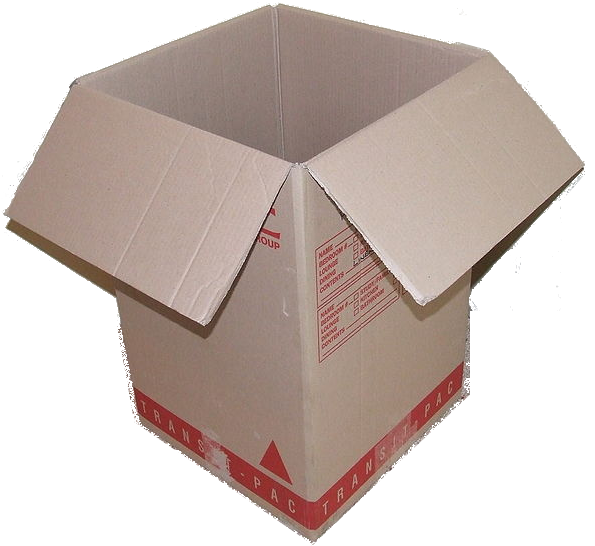
\includegraphics[width=.15\textwidth]{04/pics/box}
% XXX: no caption but label?
	\label{fig:storage-box}
\end{figure}


\section{Introduction}
\label{file systems:introduction}
\index{Storage Models}

This chapter deals primarily with how we store data.
Virtually all computer systems require some way to
store data permanently; even so-called ``diskless''
systems do require access to certain files in order to
boot, run and be useful.  Albeit stored remotely (or
in memory), these bits reside on some sort of storage
system.

Most frequently, data is stored on local hard disks,
but over the last few years more and more of our files
have moved ``into the cloud'', where different
providers offer easy access to large amounts of
storage over the network.  We have more and more
computers depending on access to remote systems,
shifting our traditional view of what constitutes a
storage device.

As system administrators, we are responsible for all
kinds of devices: we build systems running entirely
without local storage just as we maintain the massive
enterprise storage arrays that enable decentralized
data replication and archival.  We manage large
numbers of computers with their own hard drives, using
a variety of technologies to maximize throughput
before the data even gets onto a network.

In order to be able to optimize our systems on this
level, it is important for us to understand the
principal concepts of how data is stored, the
different {\em storage models} and {\em disk
interfaces}.  It is important to be aware of certain
physical properties of our storage media, and the
impact they, as well as certain historic limitations,
have on how we utilize disks.

Available storage space is, despite rapidly falling
prices for traditional hard disk drives, a scarce
resource\footnote{We will take a closer look at the
{\em Total Cost of Ownership\index{Total Cost of
Ownership}} of a hard drive in Chapter
\ref{chap:backup}.  Suffice it to say that the
purchase price of the storage device itself is only a
fraction.}.  The quote at the beginning of this chapter
is rather apt: no matter how much disk space we make
available to our users, we will eventually run out and
need to expand.  In order to accommodate the
ever-growing need for storage space, we use
technologies such as Logical Volume
Management\index{Logical Volume Manager} to combine
multiple physical devices in a flexible manner to
present a single storage container to the operating
system.  We use techniques such as
\glslink{raid}{RAID}\index{RAID} to increase capacity,
resilience, or performance (pick two!), and separate
data from one another within one storage device using
partitions.  Finally, before we can actually use the
disk devices to install an operating system or any
other software, we create a file system on top of
these partitions.

System administrators are expected to understand well
all of these topics.  Obviously, each one can (and
does) easily fill many books; in this chapter, we will
review the most important concepts underlying the
different technologies from the bottom up to the file
system level.  At each point, we will compare and
contrast traditional systems with recent developments,
illustrating how the principles, even if applied
differently, remain the same.  For significantly
deeper discussions and many more details, please see
the chapter references, in particular the chapters on
file systems in
Silberschatz\cite{filesystems:silberschatz}\index[names]{Silberschatz,
Abram} and McKusick\index[names]{McKusick, Marshall
Kirk} et al.'s canonical paper on the Berkeley Fast
File System\cite{filesystems:ffs}.


\section{Storage Models}
\label{file systems:storage-models}

We distinguish different storage models by how the
device in charge of keeping the bits in place
interacts with the higher layers: by where raw block
device access is made available, by where a file
system is created to make available the disk space as
a useful unit, by which means and protocols the
operating system accesses the file system.  Somewhat
simplified, we identify as the main three components
the storage device itself, i.e. the actual medium; the
file system, providing access to the block level
storage media to the operating system; and finally the
application software.  The operating system managing
the file system and running the application software
then acts as the agent making actual I/O possible.

\subsection{Direct Attached Storage}
\label{file systems:storage-models:das}
\index{Direct Attached Storage}

The by far most common way to access storage is so
simple that we rarely think about it as a storage {\em
model}:  hard drives are attached (commonly via a host
bus adapter\index{Host Bus Adapter} and a few cables)
directly to the server, the operating system detects
the block devices and maintains a file system on them
and thus allows for access with the smallest level of
indirection.  The vast majority of hosts (laptops,
desktop and server systems alike) all utilize this
method.  The term used nowadays -- {\em \gls{das}
\index{Direct Attached Storage}} -- was effectively
created only after other approaches become popular
enough to require a simple differentiating name.

\begin{figure}[ht]
	\centering
	\subfloat[Diagram]{\label{fig:storage:das-diagram}
			\makebox[.35\textwidth]{
				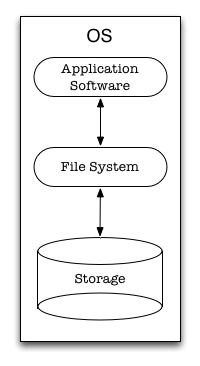
\includegraphics[width=.25\textwidth]{04/pics/das}}}
	\hspace{5em}
	\subfloat[A Maxtor IDE Drive]{\label{fig:storage:das-maxtor}
				\raisebox{2em}{
					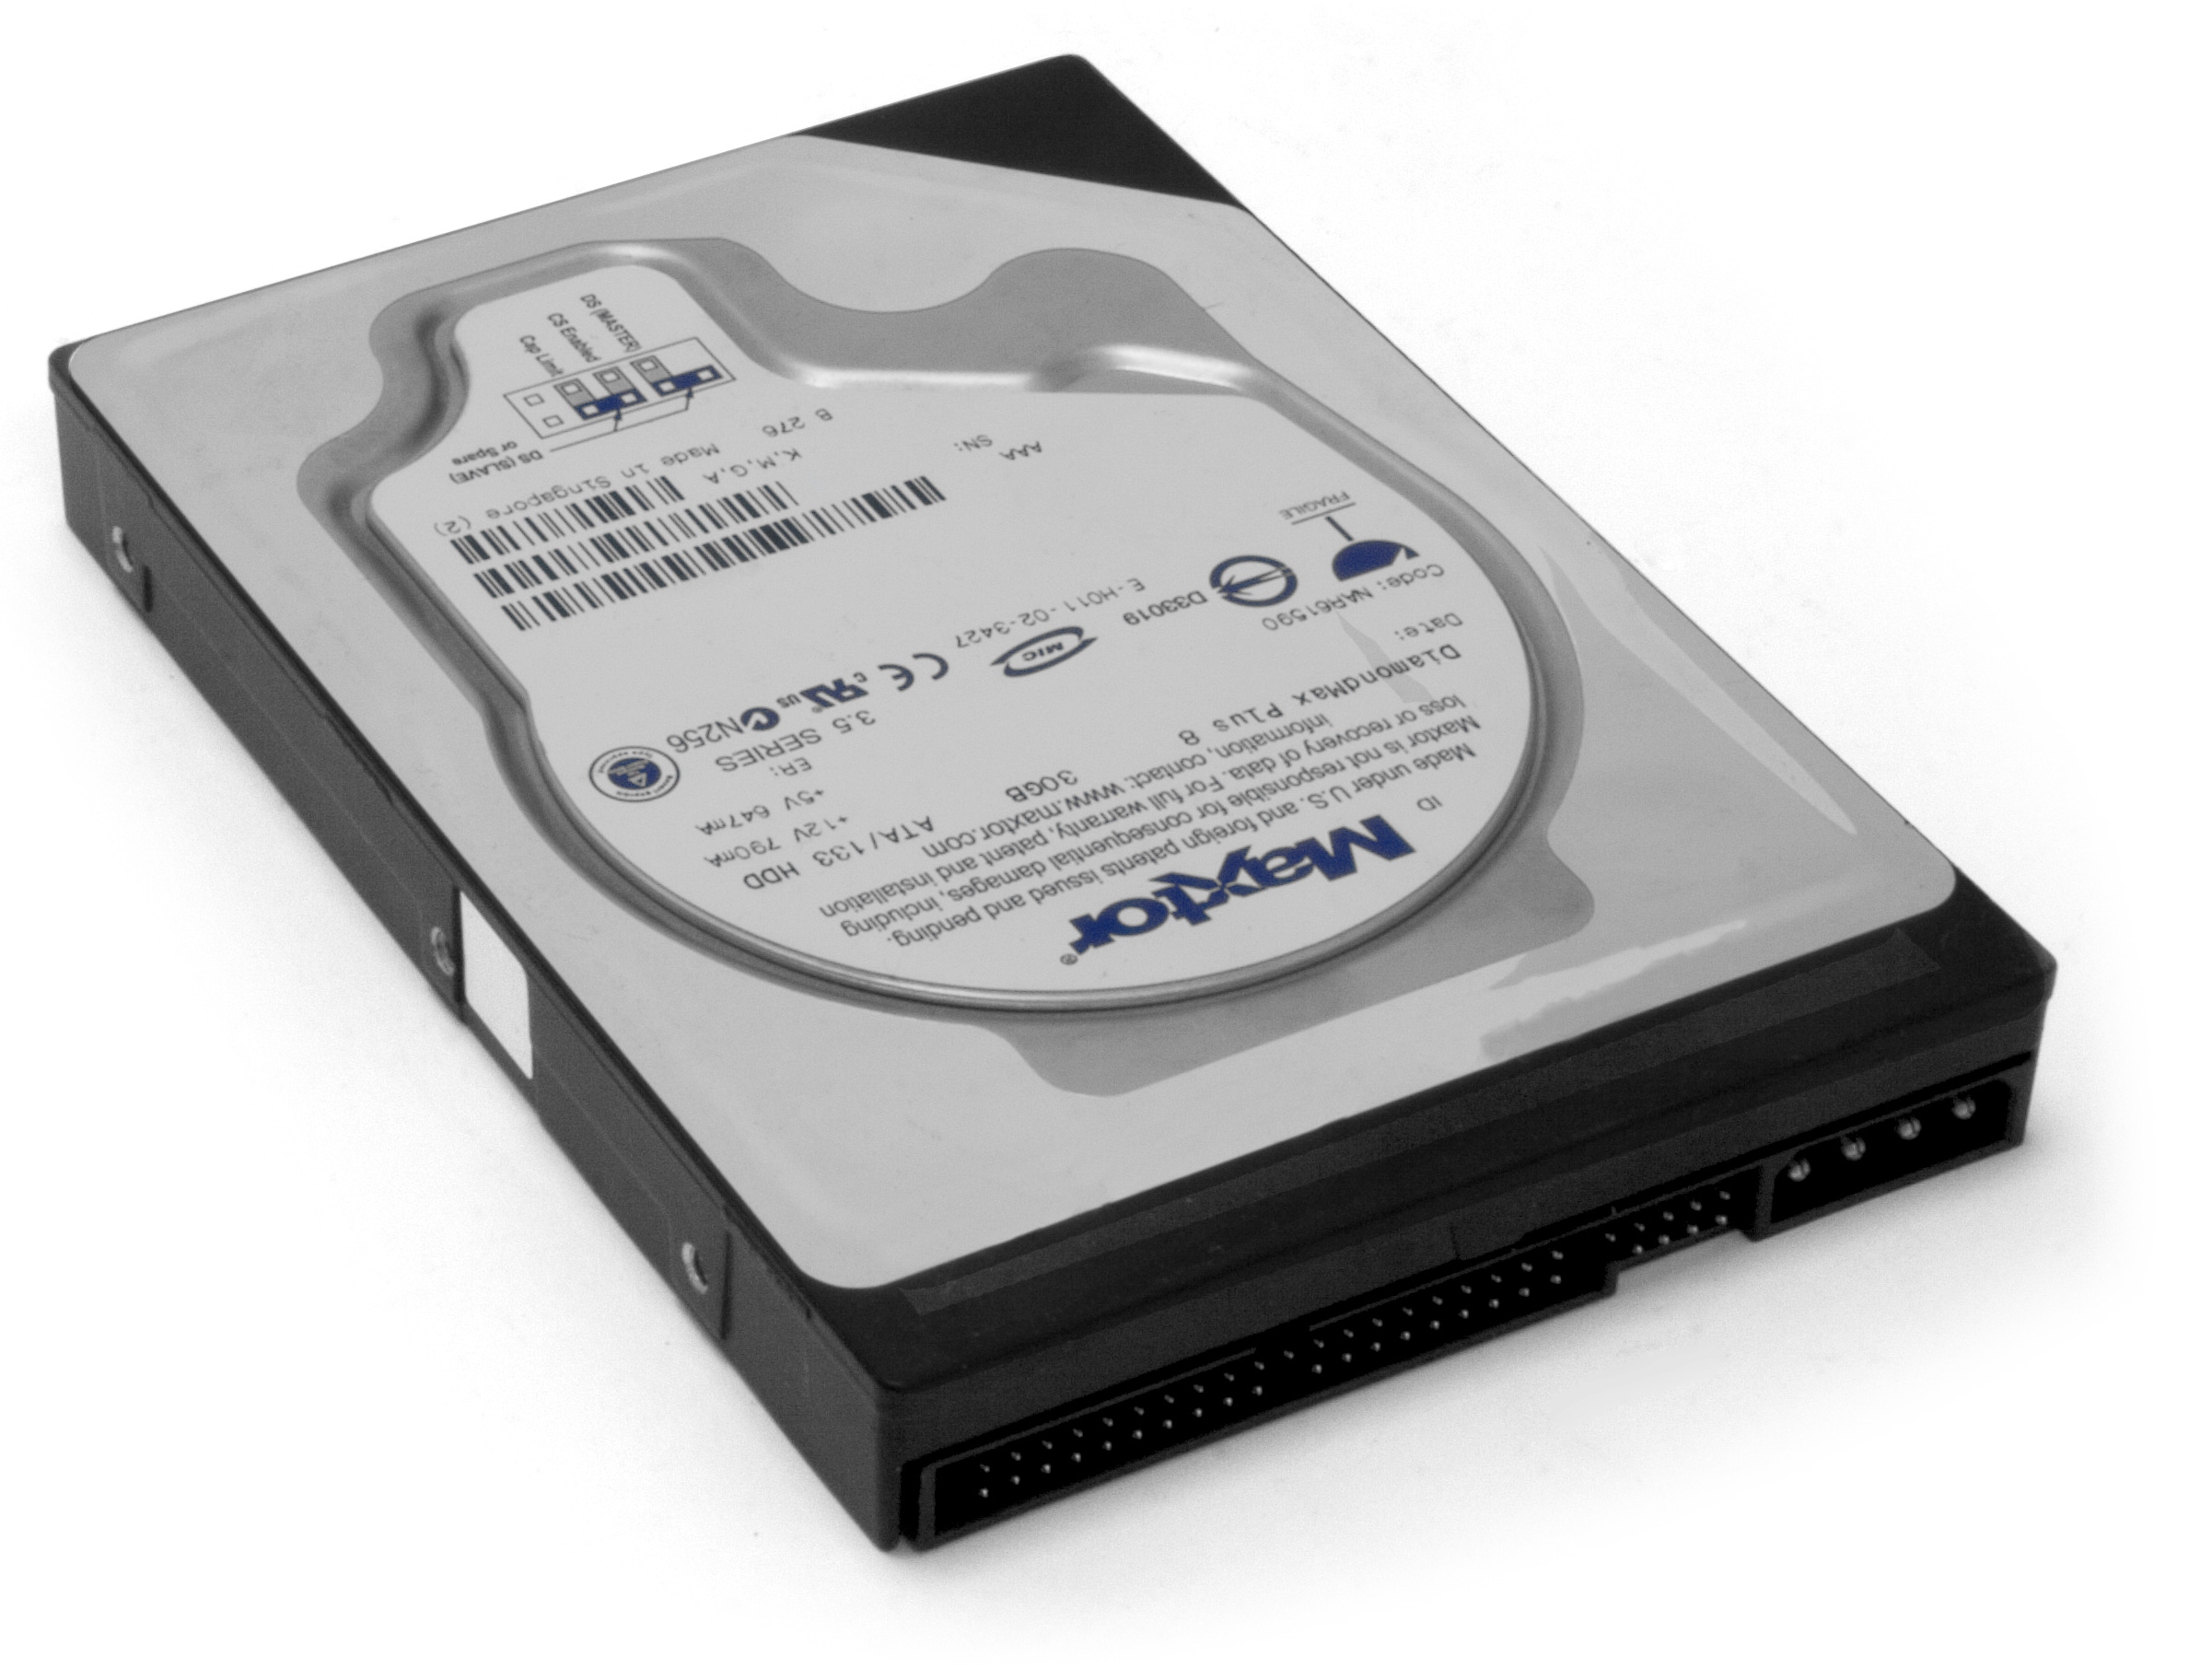
\includegraphics[width=.4\textwidth]{04/pics/maxtor}}}
	\caption{Direct Attached Storage}
\end{figure}


Figure \ref{fig:storage:das-diagram} illustrates this
model: all interfacing components are within the
control of a single server's operating system (and
frequently located within the same physical case) and
multiple servers each have their own storage system.
On the hardware level, the storage media may be
attached using a variety of technologies, and we have
seen a number of confusing standards come and go over
the years.  The best choice here depends on many
factors, including the number of devices to be
attached, driver support for the connecting interface
in the OS, and performance or reliability
considerations.  We will touch upon all of these
aspects throughout this chapter.

A server with a single hard drive (such as the one
shown in Figure \ref{fig:storage:das-maxtor} is
perhaps the simplest application of this model.  But
it is not uncommon for servers to have multiple direct
attached devices, the configuration of which then
depends entirely on the next higher level of storage
strategies.  Individual disks can simply be mounted in
different locations of the file system hierarchy.
Alternatively, multiple direct attached disks can be
combined to create a single logical storage unit
through the use of a \gls{lvm}\index{Logical Volume
Manager} or a \gls{raid}\index{RAID}.  This allows for
improved performance, increased amount of storage
and/or redundancy.  We will discuss these concepts in
more detail in Section \ref{file
systems:storage-models:dividing-and-combining-disks}.

Direct attached storage need not be physically located
in the same case (or even rack) as the server using
it.  That is, we differentiate between {\em internal}
storage (media attached inside the server with no
immediate external exposure) and {\em external}
storage (media attached to a server's interface ports,
such as Fibre Channel\index{Fibre Channel},
USB\index{USB} etc.) with cables the lengths of which
depend on the technology used.  External media allows
us to have large amounts of storage housed in a
separate enclosure with its own power supply, possibly
located several feet away from the server.  If a
server using these disks suffers a hardware failure,
it becomes significantly easier to move the data to
another host: all you need to do is connect the cable
to the new server.

Simple as this architecture is, it is also ubiquitous.
The advantages of \gls{das} should be obvious: since there
is no network or other additional layer in between the
operating system and the hardware, the possibility of
failure on that level is eliminated.  Likewise, a
performance penalty due to network latency, for
example, is impossible.  As system administrators, we
frequently need to carefully eliminate possible causes
of failures, so the fewer layers of indirection we
have between the operating system issuing I/O
operations and the bits actually ending up on a
storage medium, the better.

At the same time, there are some disadvantages.  Since
the storage media is, well, {\em directly} attached,
it implies a certain isolation from other systems on
the network.  This is both an advantage as well as a
drawback: on the one hand, each server requires
certain data to be private or unique to its operating
system; on the other hand, data on one machine
cannot immediately be made available to other systems.
This restriction is overcome with either one of the
two storage models we will review next: {\em \gls{nas}}\index{Network Attached Storage}
and {\em Storage Area Networks}\index{Storage
Area Network} (\glslink{san}{SAN}s).

\gls{das} can easily become a shared resource by
letting the operating system make available a local
storage device over the network.  In fact, all network
file servers and appliances ultimately are managing
direct attached storage on behalf of their clients;
DAS becomes a building block of {\em NAS}.  Likewise,
physically separate storage enclosures can function as
DAS if connected directly to a server or may be
combined with others and connected to network or
storage fabric, that is: they become part of a {\em
SAN}.\footnote{Don't worry, the various acronyms seem
confusing as they are introduced, but hardly anybody
actually utters sentences containing more than one.
One feels too silly doing so.}


\subsection{Network Attached Storage}
\label{file systems:storage-models:nas}
\index{Network Attached Storage}

\begin{figure}[ht]
	\centering
	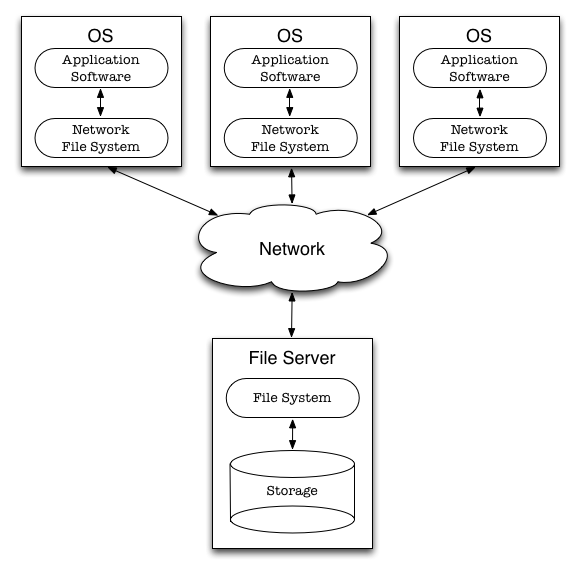
\includegraphics[width=.66\textwidth]{04/pics/nas}
		\caption{Three hosts using Network Attached Storage, or {\em NAS}
			\label{fig:storage:nas}}
\end{figure}


As the need for more and more data arises, we
frequently want to be able to access certain data from
multiple servers.  An old and still very common
example is to store all your users' data on shared
disks that are made available to all clients over the
network.  When a user logs into {\tt hostA}, she
expects to find all her files in place just as when
she logs into {\tt hostB}.  To make this magic happen,
two things are required: (1) the host's file system
has to know how to get the data from a central
location and (2) the central storage has to be
accessible over the network.  As you can tell, this
introduces a number of complex considerations, not the
least of which are access control and performance.

For the moment, let us put aside these concerns,
however, and look at the storage model from a purely
architectural point of view:  One host functions as
the ``file server'', while multiple clients access the
file system over the network.  The file server may be
a general purpose Unix system or a special network
appliance -- either way, it provides access to a
number of disks or other storage media, which, within
this system are effectively direct attached storage.
In order for the clients to be able to use the
server's file system remotely, they require support
for (and have to be in agreement with) the protocols
used\footnote{The most common protocols in use with
network attached storage solution are
\glslink{nfs}{NFS}\index{NFS} on the Unix side and
\glslink{smb}{SMB}\index{SMB}/\glslink{cifs}{CIFS}\index{CIFS}
on the Windows side.  The {\em Apple Filing Protocol}
(\glslink{afp}{AFP}\index{AFP}) is still in use in
some predominantly Mac OS environments, but Apple's
adoption of Unix for their Mac OS X operating system
made NFS more widespread there as well.}. However, the
clients do not require access to the storage media on
the block level; in fact, they {\em cannot} gain such
access.

From the clients' perspective, the job of managing
storage has become simpler:  I/O operations are
performed on the file system much as they would be on
a local file system, with the complexity of how to
shuffle the data over the network being handled in the
protocol in question.  This model is illustrated in
Figure \ref{fig:storage:nas}, albeit in a somewhat
simplified manner:  even though the file system is
created on the file server, the clients still require
support for the {\em \glslink{nfs}{network file
system}}\index{File Systems!NFS} that 
brokers the transaction performed locally with the
file server.

In contrast to \gls{das}, a dedicated file server
generally contains significantly more and larger
disks; \gls{raid} or \gls{lvm}\index{LVM} may likewise
be considered a requirement in this solution, so as to
ensure both performance and failover.  Given the
additional overhead of transferring data over the
network, it comes as no surprise that a certain
performance penalty (mainly due to network speed or
congestion) is incurred.  Careful tuning of the
operating system and in particular the network stack,
the \glslink{tcp}\index{TCP} window size, and the
buffer cache can help minimize this cost.

The benefits of using a central file server for data
storage are immediate and obvious: data is no longer
restricted to a single physical or virtual host and
can be accessed (simultaneously) by multiple clients.
By pooling larger resources in a dedicated NAS device,
more storage becomes available.

Other than the performance impact we mentioned above,
the distinct disadvantage lies in the fact that the
data becomes unavailable if the network connection
suffers a disruption.  In many environments, the
network connection can be considered sufficiently
reliable and persistent to alleviate this concern.
However, such solutions are less suitable for mobile
clients, such as laptops or mobile devices, which
frequently may disconnect from and reconnect to
different networks.  Recent developments in the area
of {\em Cloud Storage\index{Cloud Storage}} have
provided a number of solutions (see Section \ref{file
systems:storage-models:cloud}), but it should be noted
that mitigation can also be found in certain older
network file systems and protocols: the {\em
\gls{afs}}\index{AFS}, for example, uses a local
caching mechanism that lets it cope with the temporary
loss of connectivity without blocking.

While network attached storage is most frequently used
for large, shared partitions or data resources, it is
possible to boot and run a server entirely without any
direct attached storage.  In this case, the entire
file system, operating system kernel and user data
may reside on the network.  We touch on this special
setup in future chapters.

\begin{figure}[!h]
	\subfloat[Huawei Tecal RH 2288H V2]{\label{fig:storage:nas-huawei}
			\raisebox{3em}{
				\includegraphics[width=.45\textwidth]{04/pics/huawei}}}
	\hspace{5em}
	\subfloat[NetApp FAS 3050c]{\label{fig:storage:san-netapp}
				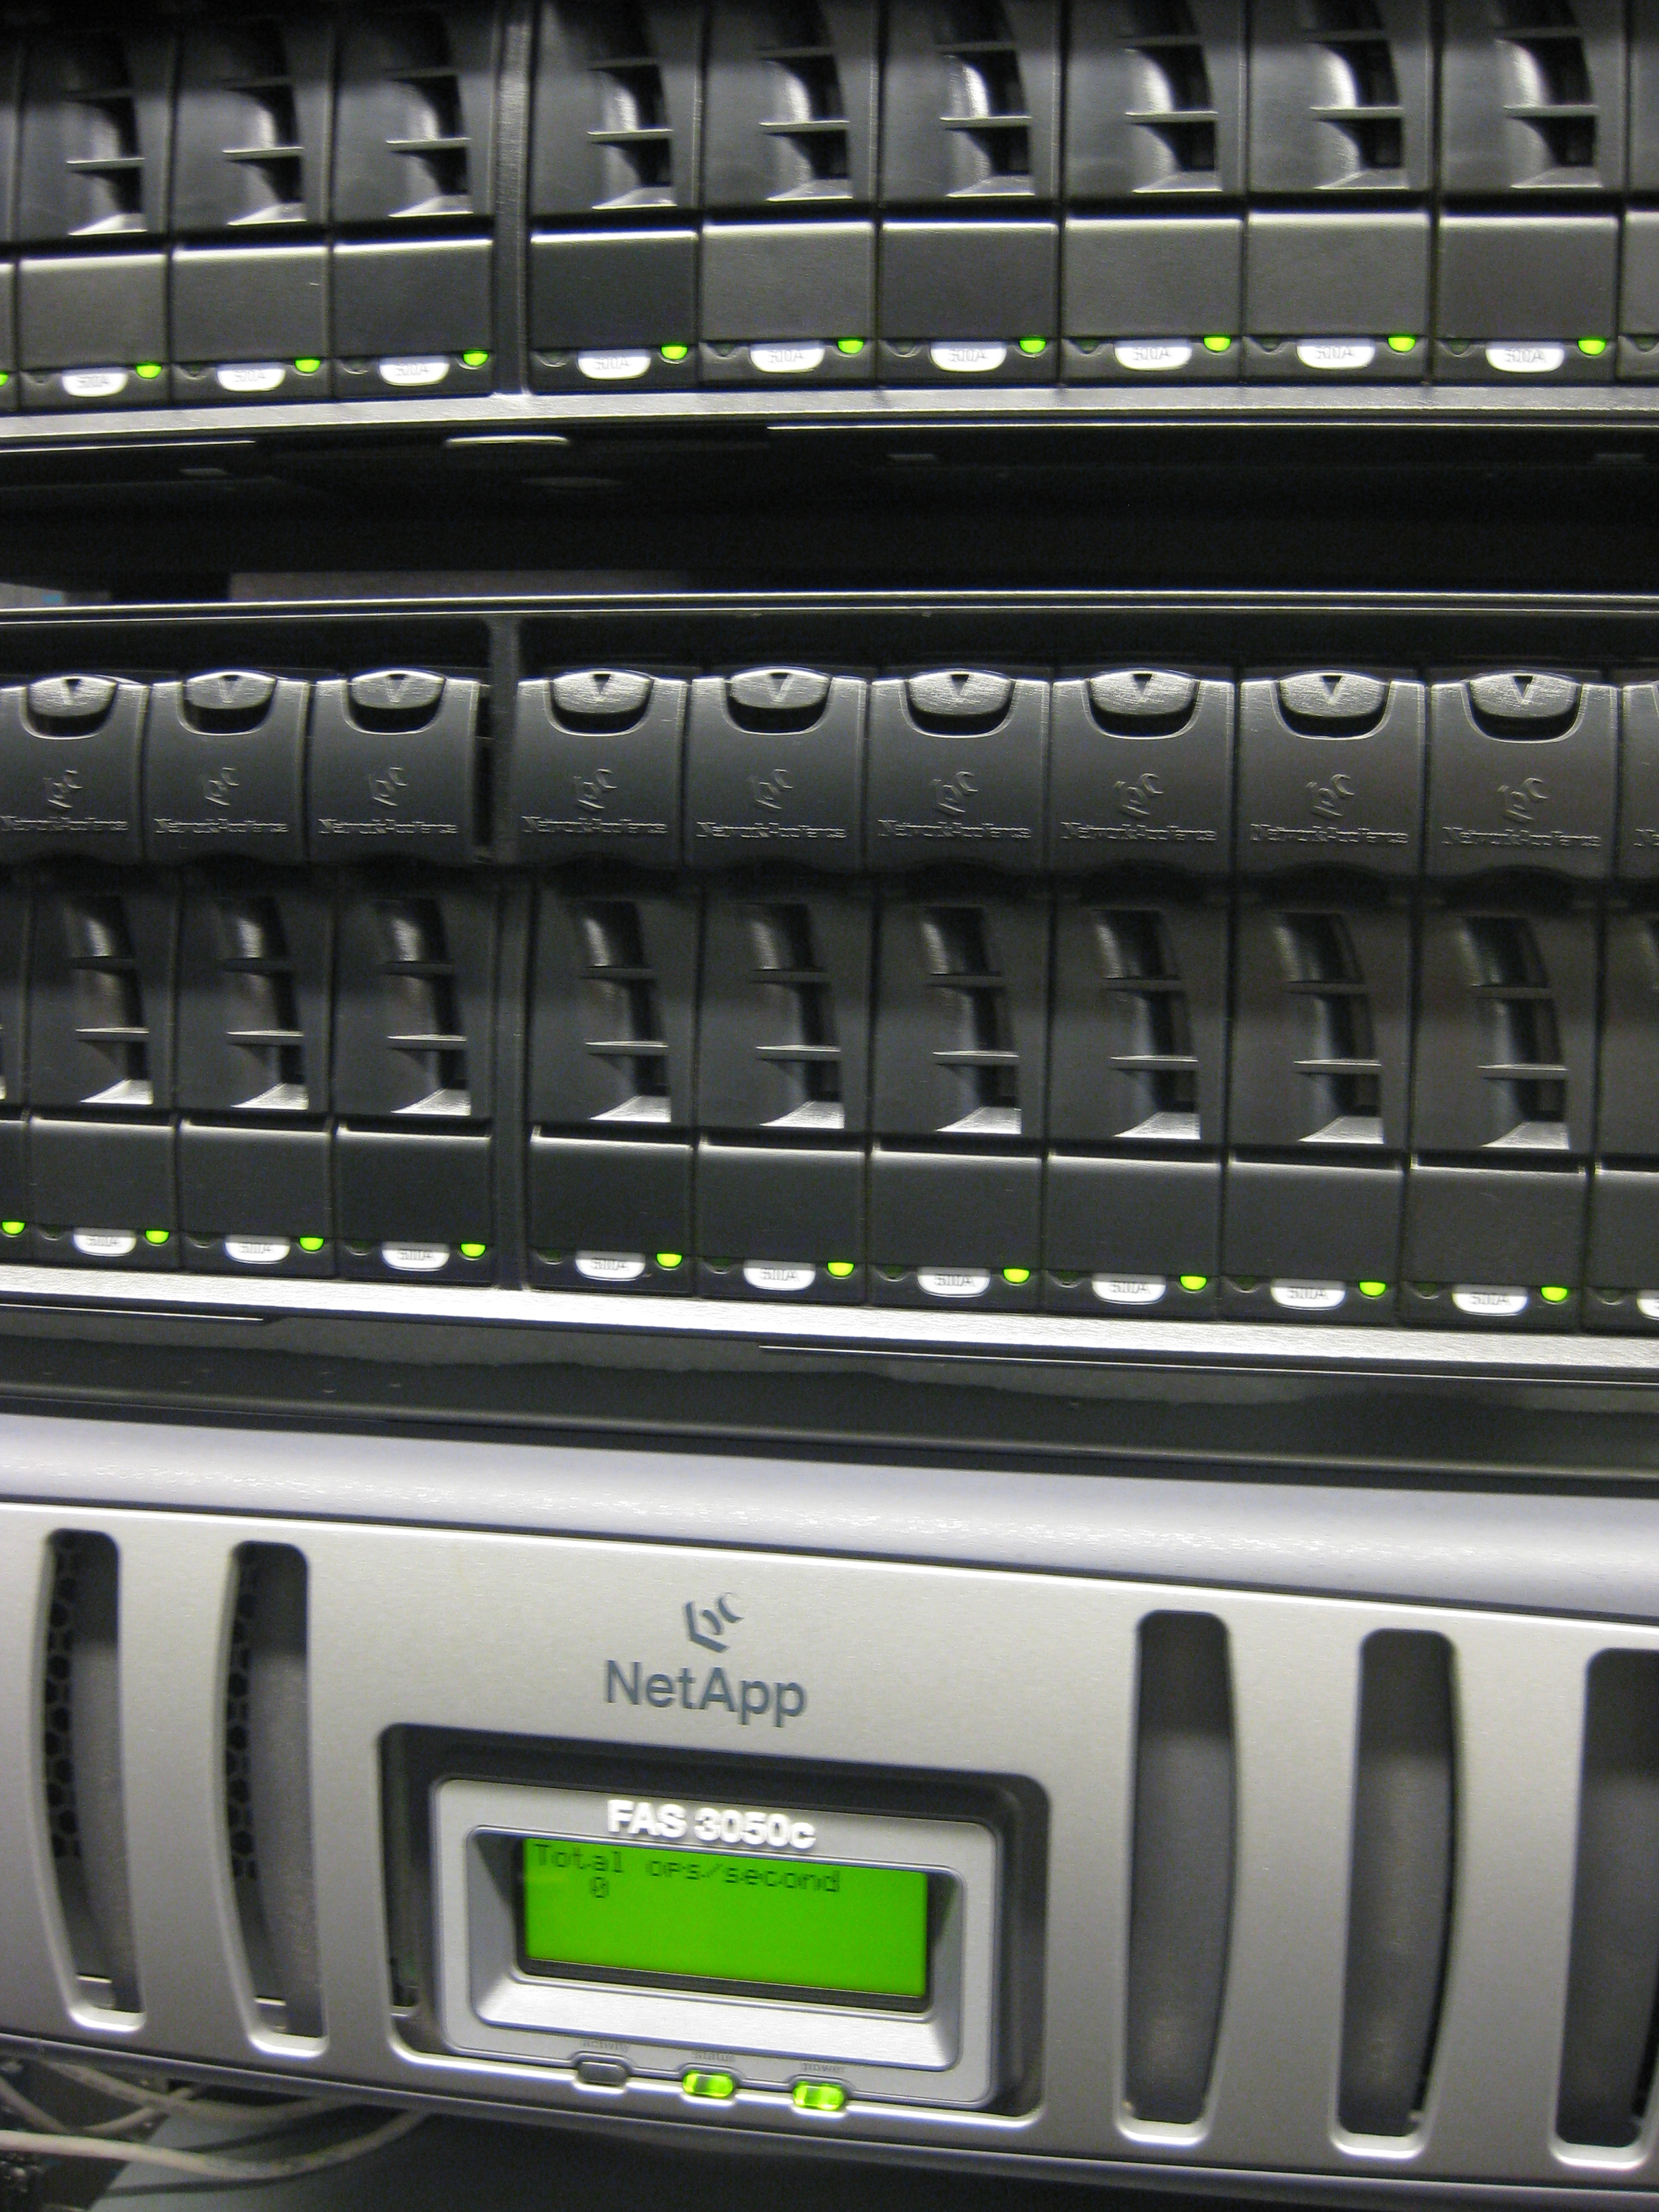
\includegraphics[width=.35\textwidth]{04/pics/netapp}}
	\caption{NAS and SAN Hardware}{NAS and SAN enterprise hardware.  On the left,
		Huawei storage servers with 24 hard
		drives each and built-in hardware RAID
		controllers; on the right, a NetApp
		Fabric Attached Storage device, also
		known as a ``filer'' with disk
		enclosures commonly referred to as ``shelves''.}
\end{figure}


\subsection{Storage Area Networks}
\label{file systems:storage-models:san}
\index{Storage Area Network}

\begin{figure}[ht]
	\centering
	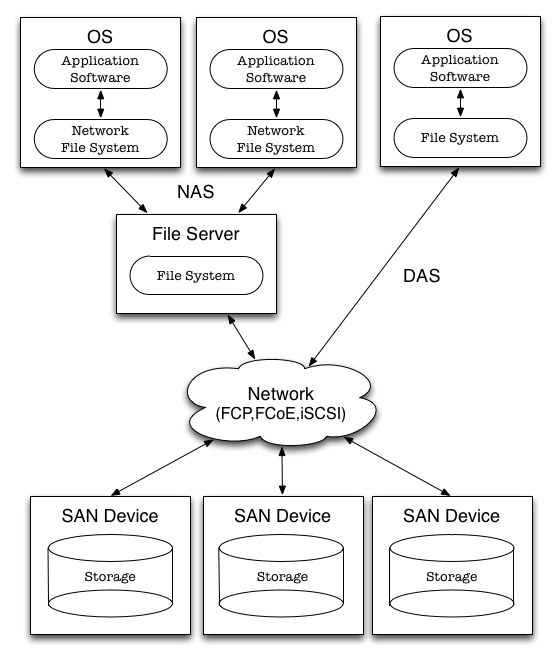
\includegraphics[width=.66\textwidth]{04/pics/san-nas-das}
		\caption[SAN illustrated]{A SAN providing access to three devices;
			one host accesses parts of the available storage
			as if it was DAS, while a file server manages
			other parts as NAS for two clients.
			\label{fig:storage:san}}
\end{figure}

\glsreset{nas}
\gls{nas} allows multiple clients to access the same file
system over the network, but that means it requires
all clients to use specifically this file system.  The
NAS file server manages and handles the creation of
the file systems on the storage media and allows for
shared access, overcoming many limitations of direct
attached storage.  At the same time, however, and
especially as we scale up, our requirements with
respect to storage size, data availability, data
redundancy, and performance, it becomes desirable to
allow different clients to access large chunks of
storage on a block level.  To accomplish this, we
build high performance networks specifically dedicated
to the management of data storage: {\em Storage Area
Networks}.\index{Storage Area Network}

In these dedicated networks, central storage media is
accessed using high performance interfaces and
protocols such as {\em Fibre Channel\index{Fibre
Channel}} or {\em iSCSI\index{iSCSI}}, making the
exposed devices appear local on the clients.  As you
can tell, the boundaries between these storage models
are not rigid: a single storage device connected via
Fibre Channel to a single host (i.e.  an example of
\gls{das}) is indistinguishable (to the client) from a
dedicated storage device made available over a
\gls{san}.  In fact, today's network file servers
frequently manage storage made available to them over
a \gls{san}\index{SAN} to export a file system to the clients as NAS.

Figure \ref{fig:storage:san} illustrates how the
storage volumes managed within a SAN can be accessed
by one host as if it was direct attached storage while
other parts are made available via a file server as
NAS to different clients.  In order for the different
consumers in a SAN to be able to independently address
the distinct storage units, each is identified by a
unique {\em \gls{lun}}.  The system administrator
combines the individual disks via RAID, for example,
into separate volumes; assigning to each storage unit
an independent LUN allows for correct identification
by the clients and prevents access of data by
unauthorized servers, an important security mechanism.
Fibre Channel switches used in SANs allow further
partitioning of the fabric by LUNs and subdivision
into SAN Zones\index{SAN Zones}, allowing sets of
clients specifically access to ``their'' storage
device only.

In this storage model the clients -- the computers,
file servers or other devices directly attached to the
SAN -- are managing the volumes on a block level (much
like a physical disk, as discussed in Section
\ref{sec:file-systems:physical-disk-structure}).  That is,
they need to create a logical structure on top of the
block devices (as which the SAN units appear), and
they control all aspects of the I/O operations down to
the protocol.  With this low-level access, clients can
treat the storage like any other device.  In
particular, they can boot off SAN attached devices,
they can partition the volumes, create different file
systems for different purposes on them and export them
via other protocols.

Storage area networks are frequently labeled an
``enterprise solution'' due to their significant
performance advantages and distributed nature.
Especially when used in a switched fabric,
additional resources can easily be made available to
all or a subset of clients.  These networks utilize
the {\em \gls{scsi}}\index{SCSI} protocol for communications
between the different devices; in order to build a
network on top of this, an additional protocol layer
-- the {\em \gls{fcp}}\index{Fibre
Channel!Protocol} being the most common
one -- is required. We will review the various
protocols and interfaces in Section \ref{file
systems:disk-devices-interface}.

SANs overcome their restriction to a {\em local} area
network by further encapsulation of the protocol: {\em
Fibre Channel over Ethernet}\index{Fibre Channel!over
Ethernet} (FCoE\index{Fibre Channel!over Ethernet}) or {\em
iSCSI}\index{iSCSI}, for example, allow connecting
switched SAN components across a Wide Area
Network\index{Wide Area Network} (or WAN).  But the
concept of network attached storage devices
facilitating access to a larger storage area network
becomes less accurate when end users require access to
their data from anywhere on the Internet.  Cloud
storage solutions have been developed to address these
needs.  However, as we take a closer look at these
technologies, it is important to remember that at the
end of the day, somewhere a system administrator is in
charge of making available the actual physical storage
devices underlying these solutions.  Much like a file
server may provide NAS to its clients over a SAN, so
do cloud storage solutions provide access on
``enterprise scale'' (and at this size the use of
these words finally seems apt) based on the foundation
of the technologies we discussed up to here.

\subsection{Cloud Storage}
\label{file systems:storage-models:cloud}
\index{Cloud Storage}

In the previous sections we have looked at storage
models that ranged from the very simple and very local
to a more abstracted and distributed approach, to a
solution that allows access across even a \gls{wan}.
At each step, we have introduced additional layers of
indirection with the added benefit of being able to
accommodate larger requirements: more clients, more
disk space, increased redundancy, etc.

We also have come full circle from direct attached
storage providing block-level access, to distributed
file systems, and then back around to block-level
access over a dedicated storage network.  But this
restricts access to clients on this specific network.
As more and more (especially smaller or mid-sized)
companies are moving away from maintaining their own
infrastructure towards a model of {\em
\gls{iaas}}\index{Infrastructure!As a Service} and
Cloud Computing\index{Cloud Computing}, the storage
requirements change significantly, and we enter the
area of {\em Cloud Storage}\footnote{Large companies are of
course also moving towards {\em IaaS}, only they
frequently are the ones simultaneously consuming as
well as {\em providing} the service, either internally
or to outside customers.}.

The term ``cloud storage'' still has a number of
conflicting or surprisingly different meanings.  On
the one hand, we have commercial services offering
{\em file hosting} or {\em file storage} services;
common well-known providers currently include Dropbox,
Google Drive, Apple's iCloud and Microsoft's SkyDrive.
These services offer customers a way to not only store
their files, but to access them from different devices
and locations: they effectively provide network
attached storage over the largest of WANs, the
Internet.

\begin{figure}[ht]
	\centering
	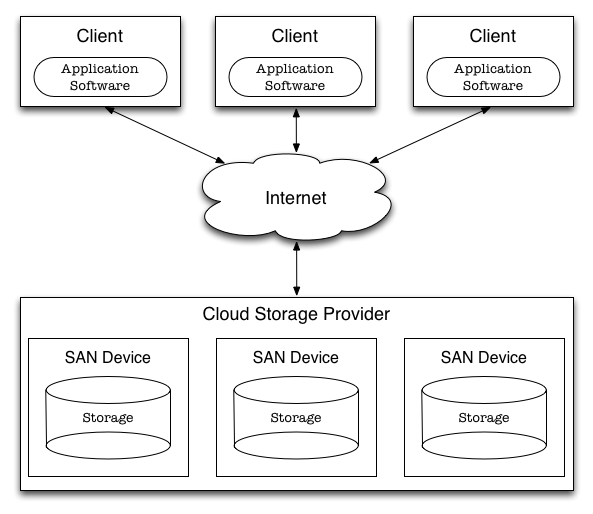
\includegraphics[width=.66\textwidth]{04/pics/cloud-storage}
		\caption[Cloud Storage]{A possible cloud storage model: an
			internal SAN is made available over the Internet to
			multiple clients.  In this example, the storage
			provider effectively functions as a NAS server,
			though it should generally be treated as a black box.
			\label{fig:storage:cloud}}
\end{figure}

On the other hand we have companies in need of a more
flexible storage solutions than can be provided with
the existing models.  Especially the increased use of
virtualization technologies demands faster and more
flexible access to reliable, persistent yet
relocatable storage devices.  In order to meet these
requirements, storage units are rapidly allocated from
large storage area networks spanning entire data
centers.

Since the different interpretations of the meaning of
``cloud storage'' yield significantly different
requirements, the implementations naturally vary, and
there are no current industry standards defining an
architecture.  As such, we are forced to treat each
product independently as a black box; system
administrators and architects may choose to use any
number of combinations of the previously discussed
models to provide the storage foundation upon which
the final solution is built.

We define three distinct categories within this
storage model: (1) services that provide file system
level access as in the case of file hosting services
such as those mentioned above; (2) services that
provide access on the {\em object level}, hiding file
system implementation details from the client and
providing for easier abstraction into an \gls{api} and
commonly accessed via web services\footnote{``Web
services'' generally expose an \gls{api} over HTTP or HTTPS
using \gls{rest}\index{REST} or the
\gls{soap}\index{SOAP}.} such as Amazon's
\gls{s3}\index{AWS!Simple Storage
Service}\index{AWS!S3}, or Windows Azure's {\em Blob}
Storage; and (3) services that offer clients access on
the block level, allowing them to create file systems
and partitions as they see fit (examples include
Amazon's \gls{ebs}\index{AWS!Elastic Block Store} and
OpenStack's\index{OpenStack} {\em Cinder} service).

All of these categories have one thing in common,
however.  In order to provide the ability of accessing
storage units in a programmatic way -- a fundamental
requirement to enable the flexibility needed in
demanding environments -- they rely on a clearly
specified \gls{api}.  Multiple distributed resources
are combined to present a large storage pool, from
which units are allocated, de-allocated, re-allocated,
relocated, and duplicated, all by way of higher-level
programs using well-defined interfaces to the
lower-level storage systems.

Customers of cloud storage solution providers reap a
wealth of benefits, including: their infrastructure is
simplified through the elimination of storage
components; storage units are almost immediately made
available {\em as needed} and can grow or shrink
according to immediate or predicted usage patterns;
applications and entire OS images can easily be
deployed, imported or exported as virtual appliances.

Of course these benefits carry a cost.  As usual, any
time we add layers of abstraction we also run the risk
of increasing, possibly exponentially, the number of
ways in which a system can fail.  Cloud storage is
no exception: by relying on abstracted storage
containers from a third-party provider, we remove the
ability to troubleshoot a system end-to-end; by
outsourcing data storage, we invite a number of
security concerns regarding data safety and
privacy\index{data privacy}; by accessing files over
the Internet, we may increase latency and decrease
throughput; the cloud service provider may become a
single point of failure for our systems, one that is
entirely outside our control.

\subsection{Storage Model Considerations}
\label{file systems:storage-models:considerations}

As we have seen in the previous sections, the larger
we grow our storage requirements, the more complex the
architecture grows.  It is important to keep this in
mind: even though added layers of abstraction and
indirection help us scale our infrastructure, the
added complexity has potentially exponential costs.
The more moving parts a system has, the more likely it
is to break, and the more spectacular its failure will
be.

A single bad hard drive is easy to replace; rebuilding
the storage array underneath hundreds of clients much
less so.  The more clients we have, the more important
it is to build our storage solution for redundancy as
well as reliability and resilience.

System administrators need to understand all of the
storage models we discussed, as they are intertwined:
\gls{das} must eventually underly any storage
solution, since the bits do have to be stored {\em
somewhere} after all; the concepts of NAS permeate any
infrastructure spanning more than just a few work
stations, and \gls{san}s\index{SAN} and cloud storage
combine DAS and NAS in different ways to make storage
available over complex networks.

At each layer, we introduce security risks, of which
we need to be aware: any time bits are transferred
over a network, we need to consider the integrity and
privacy of the files: who has access, who should
have access, how is the access granted, how are
clients authenticated, and so on.  NAS and SAN
solutions tend to ignore many of these implications
and work under the assumption that the network, over
which the devices are accessed, are ``secure''; access
controls are implemented on a higher layer such as the
implementation of the file system.  Often times,
access to the network in question implies access to
the shared storage, even though layer-2 security
mechanisms such as IPsec\index{IPsec}  may be combined
with or integrated into the solution.  Cloud storage,
on the other hand, has to directly address the problem
of transmitting data and providing access over
untrusted networks and thus usually relies on
application layer protocols such as
\gls{tls}\index{TLS}/\gls{ssl}\index{SSL}.

We will touch on some of these aspects in future
sections and chapters, but you should keep them in
mind as you evaluate different solutions for different
use cases.  As we will see, in most cases the simpler
model turns out to be the more scalable and more
secure one as well, so beware adding unneeded layers
of complexity!


\section{Disk Devices and Interfaces}
\label{file systems:disk-devices-interface}

\begin{figure}[t]
	\centering
	\subfloat[Open Hard Disc Drive]{\label{fig:file-systems:open-hard-drive}
			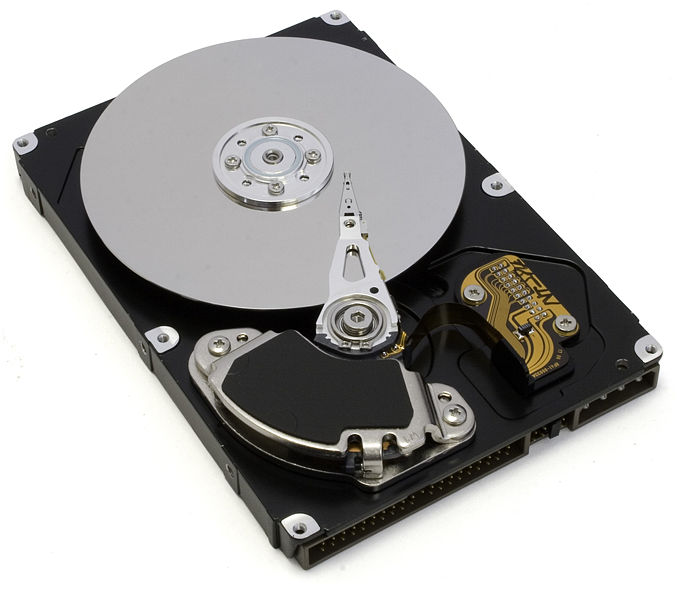
\includegraphics[width=.4\textwidth]{04/pics/open-hard-drive}}
	\hspace{7em}
	\subfloat[SSD Mini PCIe Card]{\label{fig:file-systems:ssd-mini-pcie}
			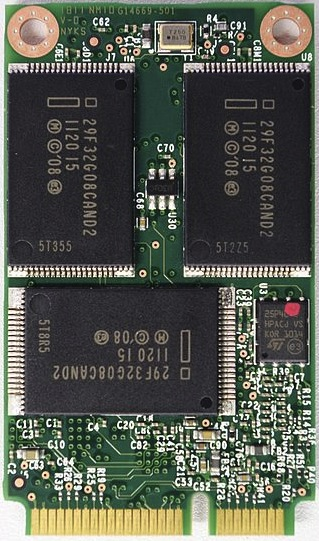
\includegraphics[width=.2\textwidth]{04/pics/ssd-minipcie}}
	\caption[HDD vs. SSD]{An open PATA (or IDE) hard drive (left) and
			a Solid State Drive (right).
			The HDD shows the rotating disk platters, the read-write
			head with its motor, the disk controller and
			the recognizable connector socket.
			\label{fig:file-systems:hdd-vs-ssd}}
\end{figure}



The different storage models we discussed in the
previous sections are just a means to access the
storage devices in order to, well, store our data.
Devices or media used to store data include tape
drives (for use with magnetic tape), optical media
such as CDs, various non-volatile memory based devices
such as flash drives,
\glslink{dram}{DRAM}\index{DRAM}-based storage, and of
course the \glslink{hdd}hard-disk drive
(HDD\index{HDD}).

Even though \gls{sdd}\index{SDD} offer significant
advantages such as lower power consumption and
generally higher performance, the dominant medium in
use especially in enterprise scale storage solutions
remains the ubiquitous hard drive\footnote{Despite
declining prices for SDDs, as of 2012 traditional hard
drives remain notably cheaper than SSDs and have
higher storage capacity.}, storing data on rotating,
magnetic platters (see Figure
\ref{fig:file-systems:open-hard-drive}).
Understanding the physical structure of these
traditional storage devices is important for a system
administrator, as the principles of especially the
addressing modes and partition schemas used here come
into play when we look at how file systems manage data
efficiently.

Hard drives can be made available to a server in a
variety of ways.  Individual disks are connected
directly to a \gls{hba}\index{Host Bus Adapter} using
a single data/control cable and a separate power
cable.  The traditional interfaces here are
\gls{scsi}\index{SCSI}, \glslink{pata}{PATA}\index{PATA} and
\glslink{sata}{SATA}\index{SATA}, as well as Fibre
Channel\index{Fibre Channel}.

SCSI, the {\em Small Computer System Interface}, has
been around for over 25 years and has seen a large
number of confusing implementations and
standards\footnote{Different SCSI versions include
such wonderful variations as {\em Fast SCSI}, {\em
Fast Wide SCSI}, {\em Ultra SCSI}, and {\em Wide Ultra
SCSI}. None of which are to be confused with {\em
iSCSI}, of course.}.  Once the default method to
connect any peripheral device using long, wide and
generally unwieldy ribbon cables, SCSI has now been
largely obsoleted by the {\em Advanced Technology
Attachment} (ATA\index{ATA}) standards.  At the same
time, however, it lives on in the {\em Internet Small
Computer System Interface} ({\em iSCSI\index{iSCSI}}),
a standard specifying storage connections using the
SCSI command protocol over IP-based networks.  iSCSI
is a common choice in storage area networks; as it
uses TCP/IP\index{TCP/IP} over existing networks, it
does not require a dedicated storage network as is the
case in traditional Fibre Channel SANs.

The {\em \gls{pata}} standard, also frequently
referred to as IDE\index{IDE} (for {\em Integrated
Device Electronics}, a reference to the fact that the
drive controller is included in the hard drive), uses
a 40 or 80 wire ribbon cable and allows for a maximum
number of two devices on the connector (traditionally
referred to as the {\em master} and {\em slave}; this
is often a source of confusion, as neither device
takes control or precedence over the other).

Faster throughput, smaller cables and support for
hot-swapping\index{hot swapping}, i.e. the ability to replace a drive
without having to shut down the operating
system\footnote{Hot-swapping was a standard feature in
many SCSI implementations.  Many system administrators
in charge of the more powerful servers, using larger
and more performant SCSI drives when compared to the
individual workstations at the time, were rather fond
of this: when a disk failed, it could be replaced
without scheduling downtime for {\em all} services.},
were some of the advantages provided by the {\em
Serial ATA} (\glslink{sata}{SATA}\index{SATA})
interface.  A number of revisions and updates to the
standard added more advanced features and, most
significantly, increasingly greater transfer speeds.

Most motherboards have integrated ATA host adapters,
but a server can be extended with additional
\glslink{hba}{HBAs} via, for example, its
\glslink{pci}{PCI} Express\index{PCI Express}
expansion slots; similarly, dedicated storage
appliances make use of disk array controllers to
combine multiple drives into logical units (more on
that in Section \ref{file
systems:storage-models:dividing-and-combining-disks}).
Fibre Channel HBAs finally allow a server to connect
to a dedicated Fibre Channel\index{Fibre Channel!SAN}
SAN.  All of these interfaces can be either internal
(the devices connected to the bus are housed within
the same physical enclosure as the server) or external
(the devices are entirely separate of the server,
racked and powered independently and connected with
suitable cables).  In the end, consider a host with a
large amount of \gls{das} and a NAS server managing
multiple terabytes of file space which is housed in
a separate device and which it accesses over a SAN:
the main difference lies not in the technologies and
protocols used, but in how they are combined. \\

\begin{advice}
{\bf Hands-on Hardware} \\
I have found it useful to have actual hardware in
class whenever possible.  In the past, I have brought
with me different hard drives by different
manufacturers and with different interfaces (PATA,
SATA, SCSI); in particular, showing students the
inside of a hard drive, the rotating platters and the
read-write arms has served as a great illustration of
the performance limiting factors, such as rotational
latency, seek time etc.  Especially old and by now
possibly obsolete hardware and the contrast in which
it stands to modern solutions is always investigated
with great interest. \\[10pt]

Likewise, a large variety of cables, connectors and
adapters help illustrate the different standards and
allow students to connect what they may have seen or
used themselves to what we talk about in class.  (See
also: Problem \ref{prob:disks:hdds})
\end{advice}

\subsection{Physical Disk Structure}
\label{sec:file-systems:physical-disk-structure}

Let us open up a typical hard drive and take a look at
the physical structure.  This will help us better
understand the concepts of partitions, how the
operating system calculates the disk geometry and
allocates physical blocks, how the file system manages
cylinder groups\index{cylinder groups}, and why, for
example, storing data on the outer disk blocks could
improve performance.

If you open a traditional hard-disk drive and manage
not to destroy it completely in the process, you will
look at a number of magnetic platters on a spindle
together with the read-write heads.  The other main
components include the disk motor (spinning the
platters), an actuator (moving the read-write heads)
and the disk controller.

The platters are coated on both surfaces with magnetic
particles, allowing us to store on (and retrieve off)
them data in the form or zeros and ones by polarizing
the relevant area.  The read-write heads -- one for
each platter surface -- may be resting on the {\em
landing zone} near the spindle; they do not touch the
platters when they are rotating.  Instead, they hover
just above the platters and are moved radially across
the disks by the actuator to position them at the
desired location.  If the read-write heads are brought
into contact with the spinning platters, the results
tend to be rather disastrous, as the magnetic surface
of the disk is damaged by this {\em head
crash}\index{head crash}.

\begin{figure}[ht]
	\centering
	\subfloat[Disk Structure: Cylinders/Tracks, Heads, Sectors]{
			\label{fig:file-systems:chs}
			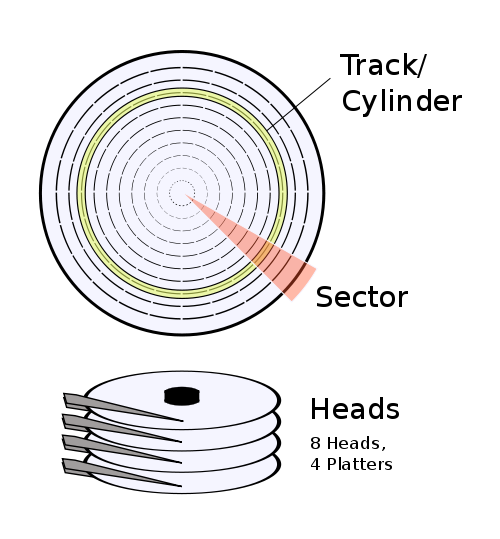
\includegraphics[width=.4\textwidth]{04/pics/chs}}
	\hspace{1em}
	\subfloat[Physical Disk Structure with Zone Bit Recording]{
			\label{fig:file-systems:disk-structure-zbr}
			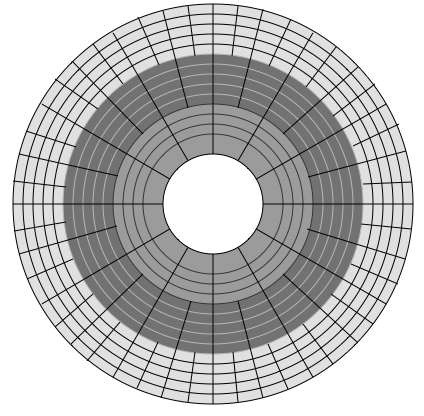
\includegraphics[width=.4\textwidth]{04/pics/disk-structure-zone-bit-recording}}
	\caption[Physical Disk Structure]{On the left: Illustration of tracks and sectors
			on a hard disk.  Note that for simplicity,
			sectors on the inside and outside
			of the platters are of identical size.  On
			disks with Zone Bit Recording\index{Zone Bit Recording}
			(shown on the right), this is no longer the case.}
\end{figure}


The surface of each platter is divided into concentric
rings, or {\em tracks}.  Congruent tracks on multiple
platters form a three-dimensional {\em cylinder}.
Within a single cylinder, data can be read from all
available surfaces without requiring the read-write
heads to move.  This is why {\em disk
partitions}\index{partition} comprise multiple
cylinder groups\index{cylinder groups} rather than, as
we may sometimes imagine them to be, pie wedges.


The tracks on each platter are in turn divided into a
number of {\em sectors}.  If you were to divide a disk
with concentric tracks by drawing straight lines from
the center to the outer edge, you would quickly
realize that even though you end up with the same
number of such sectors on each track, the fields
created in this manner would be of varying sizes:  the
ones on the outer edge would be significantly larger
than the ones in the middle of the disc (see Figures
\ref{fig:file-systems:chs} and
\ref{fig:file-systems:disk-structure-zbr}).

As these fields represent the smallest addressable
unit on a hard drive, we would be wasting a lot of
disk space.  Instead, each sector is kept at a fixed
size\footnote{The industry standard for hard drives
used to be 512 bytes for many years; since around
2010, a number of vendors have started creating hard
drives with a physical block size of 4096 bytes.
Interestingly, file systems having standardized on 512
byte blocks tend to divide these blocks and continue
to present to the OS 512 byte ``physical'' blocks.}
and use a technique known as {\em Zone Bit
Recording}\index{Zone Bit Recording} to store more
sectors on the outer tracks of each disc than on the
inner area.

The total number of 512 byte sectors across all
platters of the hard drive thus define its total
capacity.  In order to access each storage unit, the
read-write head needs to be moved radially to the
correct cylinder -- a process we call {\em seeking} --
and the platter then spun until the correct sector is
positioned under it.  In the worst case scenario, we
just passed the sector we wish to access and we have
to perform a full rotation.  Therefore, a drive's
performance is largely defined by this {\em rotational
latency}\index{rotational latency} and the time to
position the read-write head (also known as {\em seek
time}).

Since the motor of a drive may rotate the discs at a
constant linear velocity (versus constant angular
velocity), the discs are in fact moving slower near
the spindle than on the outer part.  This means that
more sectors could be read in a given time frame from
the outside of the discs than from the inside.  In
fact, it used to be not uncommon for system
administrators to partition their disks such that
large, frequently accessed files would reside on
cylinders near the beginning (i.e. the outside) of the
platters.  Nowadays such fine tuning may no longer be
common, but instead people have started to simply
create a single partition occupying only about 25\% of
the disk at the beginning and ignoring the rest.  This
technique, known as ``{\em short stroking}\index{short
stroking}'', may seem wasteful, but the performance
gain compared to the cheap prices of today's HDDs may
make it actually worthwhile.

It is worth noting that the physical disk structure
described here applies only to traditional mechanical
hard drives, not to Solid State Drives\index{Solid
State Drive} or other storage media.  Nevertheless, it
is useful to understand the structure, as a number of
file system or partitioning conventions derive
directly from these physical restrictions.

\begin{sidenote}
{\bf True Hard Drive Capacity} \\
Hard drive manufacturers use a different definition of
what constitutes a Gigabyte than is customary pretty
much anywhere else: normally, we define computer
storage in terms of powers of two.  That is, a
kilobyte is commonly understood to be $2^{10}$ bytes,
a megabyte $2^{20}$ and a gigabyte $2^{30}$.  In
contrast, the standard prefix {\em giga} means $10^9$,
and hard drive manufacturers use this meaning.  Some
people differentiate between these conflicting
definitions by using the term {\em Gibibyte} (GiB) for
$2^{30}$ bytes, but even though technically correct,
this term has never really caught on. \\[10pt] As a
result, a drive labeled as having a capacity of 500 GB
will in fact only be able to store around 465 GiB.
The larger the drive, the bigger the difference - at
1TB ($2^{40}$ versus $10^{12}$), you are getting a
full 10\% less storage than advertized!
\end{sidenote}

\section{Dividing and Combining Disks}
\label{file systems:storage-models:dividing-and-combining-disks}

Disk space is a finite and fixed resource.  Each hard
drive we purchase has a given capacity, and it is up
to the system administrators to use it efficiently.
In this section, we will take a look at the
different methods to provide the optimal amount of
storage space to your systems.  Sometimes this
involves dividing a single hard drive into multiple
partitions; other times, we want to combine multiple
hard drives to increase capacity, yet retain a logical
view of the storage space as a single unit.  Finally,
the ways in which we divide or combine disks have
implications on system performance and data
redundancy.



\subsection{Partitions}
\label{file systems:storage-models:dividing-and-combining-disks:partitions}
\index{Disks!Partitions}

Now that we understand the physical layout of the hard
disks, we can take a look at how we {\em partitions}
are created and used.  As we noted in the previous
section, a disk partition is a grouping of adjacent
cylinders through all platters of a hard
drive\footnote{Some operating systems such as Solaris,
for example, have traditionally referred to partitions
as ``slices''; some of the BSD systems also refer to
disk ``slices'' within the context of {\em
\glslink{bios}{BIOS} partitions}.  Unfortunately, this
easily brings to mind the misleading image of a slice
of pie, a wedge, which misrepresents how partitions
are actually laid out on the disk.}.  Despite this
unifying principle, we encounter a variety of
partition types and an abundance of related
terminology: there are {\em partition
tables\index{partition!table}} and {\em disklables},
{\em primary}\index{partition!primary} and {\em
extended}\index{partition!extended} partitions; there
are whole-disk partitions, disks with multiple
partitions, and some of the partitions on a disk may
even overlap.

Different file systems and anticipated uses of the
data on a disk require different kinds of partitions.
First, in order for a disk to be bootable, we require
it to have a {\em boot sector}\index{boot sector}, a
small region that contains the code that the
computer's firmware (such as the
\gls{bios}\index{BIOS}) can load into memory.  In
fact, this is precisely what a BIOS does: it runs
whatever code it finds in the first sector of the
device so long as it matches a very simple boot
signature\index{boot signature}.  That is, regardless
of the total capacity of the disk in question, the
code that chooses how or what to boot needs to fit
into a single sector, 512 bytes.  On most commodity
servers\footnote{Even though many other hardware
architectures used to be dominant in the server
market, nowadays the {\em x86} instruction set (also
known as ``IBM PC-compatible'' computers) has replaced
most other systems.  For simplicity's sake, we will
assume this architecture throughout this chapter.},
this code is known as the {\em Master Boot
Record}\index{Master Boot Record} or MBR\glslink{mbr}.
In a classical MBR the last two bytes of this sector
contain the signature {\tt 0x55 0xAA}; bootstrap code
area itself takes up 446 bytes, leaving 64 bytes of
space.  At 16 bytes per partition entry, we can have
at most four such {\em BIOS
partitions}\index{Partitions!BIOS} that the MBR can
transfer control to.

\begin{lstlisting}[float,label=code:fdisk,caption=fdisk(8) sample invocation
and output on a Linux system]
# fdisk -l
Disk /dev/cciss/c0d0: 73.3 GB, 73372631040 bytes
255 heads, 63 sectors/track, 8920 cylinders
Units = cylinders of 16065 * 512 = 8225280 bytes

           Device Boot Start   End    Blocks   Id  System
/dev/cciss/c0d0p1   *      1  2550  20482843+  83  Linux
/dev/cciss/c0d0p2       2551  7649  40957717+  83  Linux
/dev/cciss/c0d0p3       7650  7904   2048287+  82  Linux swap
#
\end{lstlisting}

Sometimes you may want to divide the available disk
space into more than four partitions.  In order to
accomplish this, instead of four {\em primary}
partitions, the \gls{mbr} allows you to specify three
primary and one so-called {\em extended} partition,
which can be subdivided further as needed.  When the
system boots, the \gls{bios} will load the MBR code, which
searches its partition table for an ``active''
partition, from which it will then load and execute
the boot block.  This allows the user to run multiple
operating systems from the same physical hard drive,
for example.  BIOS partitions are usually created or
maintained using the {\tt fdisk(8)}\index{\tt fdisk(8)}
utility.

\begin{sidenote}
{\bf Disk and BIOS Limitations} \\

In order to address sectors of a hard drive, computers
used the {\em
\gls{chs}}\index{Addressing!Cylinder-Head-Sector}
scheme.  Early BIOSes were only able to address 1024
cylinders, 256 heads and 63 sectors/track.  At the
same time, the ATA specification for IDE disks defined
a limit of 65536 cylinders, 16 heads, and 256 sectors.
As a result, the lowest common denominator required
addressing -- and thus total disk sizes -- to be
limited to:\\ [10pt]

$1024 (cylinders) * 16 (heads) * 63 (sectors) * 512 (bytes / sector) = 504 MB $ \\[10pt]

{\em Enhanced BIOS}es removed some of these
limitations, allowing for disks with an at that time
impressive size of approximately 8 GB ($1024 * 255 *
63 * 512$).  But they were only able to access the
first 1024 cylinders of a disk.  This meant that all
the files required to boot the OS (which then might be
able to address more disk space) had to reside within
these cylinders.  As a result, many Unix systems have
a default partitioning scheme including a small {\tt
/boot} partition created at the beginning of the disk.
\\ [10pt]

To overcome the limitations of
\gls{chs}\index{Addressing!Cylinder-Head-Sector}
addressing, data blocks on the disks were simply
numbered and counted, yielding {\em
\gls{lba}}\index{Addressing!Logical Block}.  Using
this method, IDE disks could thus address however many
blocks it could store in the data type it used for
this purpose; the ATA specification used 28 bits, and
thus imposed a limit of $(2^{28}\,sectors * 512\,
bytes/sector)/1024^3\, bytes/GB = 128\, GB$ (or
$~137.4GiB$ at $10^9\, bytes/GiB$). \\ [10pt]

In 2012, the current ATA/ATAPI\index{ATA}
specification uses 48 bits, limiting disk size to 128
Petabytes (PB); however, some operating systems still
use 32 bits to address sectors, so that on those
systems the largest supported disk size is 2 Terabyte
(TB), yet another limitation we now run into and which
may seem laughably small in just a few years.
\end{sidenote}


Just as the first sector of the disk contains the
\gls{mbr}, so does the first sector of a \gls{bios}
partition contain a {\em volume boot
record}\index{volume boot record}, also known as a
{\em partition boot sector}\index{partition boot
sector}.  In this sector, the system administrator may
have placed a second-stage
bootloader\index{bootloader}, a small program that
allows the user some control over the boot process by
providing, for example, a selection of different
kernels or boot options to choose from.  Only one
partition is necessary to boot the OS, but this
partition needs to contain all the libraries and
executables to bootstrap the system.  Any additional
partitions are made available to the OS at different
points during the boot process.

\begin{lstlisting}[basicstyle=\scriptsize,float,label=code:disklabel,caption=disklabel(8)
invocation and output on a NetBSD system]
# dmesg | grep xbd3
xbd3 at xenbus0 id 3: Xen Virtual Block Device Interface
xbd3: 24575 MB, 512 bytes/sect x 50331520 sectors
# disklabel /dev/xbd3
type: ESDI
disk: Universal Swap
label: disk1
bytes/sector: 512
sectors/track: 306432
tracks/cylinder: 1
sectors/cylinder: 306432
cylinders: 255
total sectors: 78140160
rpm: 3600
interleave: 1

8 partitions:
#      size   offset fstype [fsize bsize cpg/sgs]
a: 20972385       63 4.2BSD   4096 32768    1180  # (Cyl.     0*- 20805)
b:  1048320 20972448   swap                       # (Cyl. 20806 - 21845)
c: 78140097       63 unused      0     0          # (Cyl.     0*- 77519)
d: 78140160        0 unused      0     0          # (Cyl.     0 - 77519)
e: 56119392 22020768 4.2BSD   4096 32768   58528  # (Cyl. 21846 - 77519)
#
\end{lstlisting}


In the BSD family of operating systems, the volume
boot record contains a {\em disklabel}, detailed
information about the geometry of the disk and the
partitions it is divided into.  Listing
\ref{code:disklabel} shows the output of the {\tt
disklabel(8)}\index{\tt disklabel(8)} command on a
NetBSD\index{NetBSD} system.  You can see the
breakdown of the disk's geometry by cylinders, sectors
and tracks and the partitioning of the disk space by
sector boundaries.  This example shows a 40
GB\footnote{$ (78140160\, sectors * 512\, bytes/sector) /
(1024^3\, bytes/GB) = 37.26\, GB$ \\ Note the difference
in actual versus reported disk size: \\ $(40*2^{30} -
40*10^9)/(1024^3) = 40 - 37.26 = 2.74$ } disk
containing three partitions, a 10 GB root partition, a
512 MB swap partition and a data partition comprising
the remainder of the disk.  Since the disk in question
is actually a virtual disk, the information reported
relating to the hardware, such as the {\tt rpm} rate,
for example, is obviously wrong and should be ignored.
This serves as a reminder that a system
administrator always may need to have additional
background knowledge (``this host is a virtual machine
with a virtual disk'') to fully understand the output
of her tools in order to make sense of it.  Note also
that some partitions overlap.  This is not a mistake:
the BSD disklabel includes information about both the
entire disk (partition '{\tt d}') as well as the
\gls{bios} partition assigned to NetBSD (partition '{\tt
c}', starting at offset {\tt 63}).  Other partitions,
i.e.  partitions actually used by the OS, should {\em
not} overlap.

Being able to read and understand the detailed output
of these commands is important, and students are
encouraged to practice making sense of different
partition schemas across different operating systems
(see exercise \ref{prob:disks:disklabel}). \\

Dividing a single large disk into multiple smaller
partitions is done for a number of good reasons: if
you wish to install multiple operating systems, for
example, you need to have dedicated disk space as well
as a bootable primary partition for each OS.  You may
also use partitions to ensure that data written to one
location (log files, for example, commonly stored
under e.g. {\tt /var/log}) cannot cause you to run out
of disk space in another (such as user data under {\tt
/home}).  Other reasons to create different partitions
frequently involve the choice of file system or mount
options, which necessarily can be applied only on a
per-partition basis.  We will discuss a number of
examples in Section \ref{sec:file systems}.

\subsection{Logical Volumes}
\label{file systems:storage-models:dividing-and-combining-disks:logical-volumes}
\index{Logical Volumes}

Using hard drives with fixed partitions may lead to a
number of problems: disk drives are prone to hardware
failure, which may lead to data loss; reading data
from individual disk drives may suffer performance
penalties depending on the location of the data on the
disk; and, perhaps most notably, disks are never large
enough.

Partitions are a good way to divide a single disk and
make available to the OS smaller, distinct units of
storage.  But throughout the life time of our systems,
we frequently have a need to {\em increase} storage
space -- consider the quote from the beginning of this
chapter: ``{\em Data expands to fill any void.}''  We
can buy a larger hard drive and add it to the system
and then migrate data to it or simply mount it in a
separate location\footnote{An approach aptly
described as ``\glslink{jbod}{JBOD}\index{JBOD}'':
``Just a Bunch Of Disks''.}, but neither solution is
particularly elegant.  The problem here is that
partitions are fixed in size throughout their life
time.  Wouldn't it be nice if we could simply combine
the storage from multiple disk drives and then create
partitions spanning the total?

Enter {\em logical volumes}.  Much like a
\gls{san}\index{SAN} may combine multiple storage
devices and make them available to its clients, so
does a logical volume manager (or
\gls{lvm}\index{LVM}) combine multiple physical
devices and present them to the OS as a single
resource.  In this case, the abstraction occurs on the
device-driver level; some advanced file systems may
include aspects of an LVM (see ZFS\index{ZFS}'s
\manpage{zpool(1)} command, for example).

\begin{figure}[ht]
	\centering
	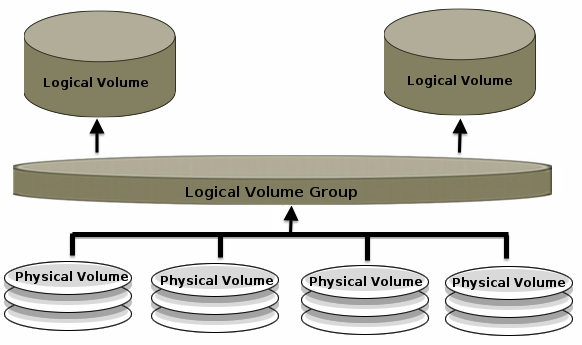
\includegraphics[width=.75\textwidth]{04/pics/lvm}
		\caption[Logical Volume Management]{Logical Volume
			Management lets you combine multiple physical disks
			or partitions into a single {\em volume group},
			from which {\em logical volumes} can be allocated.
			\label{fig:file-systems:lvm}}
\end{figure}



The management of the locally attached storage devices
via so-called {\em logical volume groups} grants the
system administrator a significant amount of
flexibility: the total storage space can
easily be extended (and the file system, if it
supports this operation, grown!) by adding new disk
drives to the pool; file system performance can be
improved by {\em striping} data across all available
drives; data redundancy and fault tolerance can be
improved by {\em mirroring} data on multiple devices.
These last two advantages are also provided by the
\gls{raid} storage solution, which we will look at in more
detail in the following section. \\

\gls{lvm}s manage and combine three distinct
resources, as illustrated in Figure
\ref{fig:file-systems:lvm}: {\em physical volumes},
{\em logical volume groups} and {\em logical volumes}.
A physical volume can be a hard disk, a partition on a
hard disk, or a logical unit number of a local or
remote device (such as SAN connected storage device).
The LVM divides the physical volumes into data blocks,
so-called {\em physical extents}\index{LVM!physical
extent}, and allows the system administrator to group
one or more of these physical volumes into a logical
volume group.  In effect, available storage space is
combined into a pool, where resources can dynamically
be added or removed.  Out of such a volume group,
individual logical volumes can then be created, which
in turn are divided into the equivalent of a hard
disk's sectors, so-called {\em logical
extents}\index{LVM!logical extent}.  This step of
dividing a logical volume group into logical volumes
is conceptually equivalent to the division of a single
hard drive into multiple partitions; in a way, you can
think of a logical volume as a virtual disk.  To the
operating system, the resulting device looks and
behaves just like any disk device: it can be
partitioned, and new file systems can be created on
them just like on regular hard drive disks.

By creating logical extents as storage units on the
logical volumes, the LVM is able to grow or shrink
them with ease (the data corresponding to the logical
extends can easily be copied to different physical
extents and remapped), as well as implement data
mirroring (where a single logical extent maps to
multiple physical extents).

Since logical volume management is a software solution
providing an additional layer of abstraction between
the storage device and the file system, it can provide
additional features both on the lower level, such as
data mirroring or striping, as well as on a higher
level, such as file system snapshots\index{snapshots},
which an \gls{lvm} can easily implement using a
``copy-on-write''\index{Copy-on-Write} approach when
updating the logical extents.  We will discuss this
topic in more detail in our chapter on backups in
Section \ref{backup:file-system-backups}.

Note that some of the desirable features of logical
volume management are not entirely independent of the
higher file system layer.  For example, a change in
size of the logical volumes requires the file system
to adapt, and growing a file system to expand to
consume additional disk space is often easier than
shrinking the file system.  Hence, the choice to use
an \gls{lvm} needs to be coupled with the ``right'' file
system!

\subsection{RAID}
\label{file systems:storage-models:dividing-and-combining-disks:raid}
\index{RAID}

Logical Volume Managers provide a good way to
consolidate multiple disks into a single large storage
resource from which individual volumes can be created.
An \gls{lvm} may also provide a performance boost by
striping data, or redundancy by mirroring data across
multiple drives.

Another popular storage technology used for these
purposes is {\em RAID}, which stands for {\em
Redundant Array of Independent Disks}\footnote{The
acronym ``\gls{raid}'' is sometimes expanded as ``Redundant
Array of {\em Inexpensive} Disks''; since disks have
become less and less expensive over time, it has
become more customary to stress the ``independent''
part.  A cynic might suggest that this change in
terminology was driven by manufacturers, who have an
interest in not explicitly promising a low price.}.
Multiple disks can be combined in a number of ways to
accomplish one or more of these goals: (1) increased
total disk space, (2) increased performance, (3)
increased data redundancy.

Much like an \gls{lvm}, RAID as well hides the
complexity of the management of these devices from the
OS and simply presents a virtual disk comprised of
multiple physical devices.  However, unlike with
logical volume management, a RAID configuration cannot
be expanded or shrunk without data loss.  Furthermore,
an \gls{lvm}is a software solution; RAID can be
implemented on either the software or the hardware
layer.  In a hardware RAID\index{RAID!Hardware}
solution, a dedicated disk array controller (such as a
PCI\glslink{pci} card) is installed in the server, and
interacted with via controlling firmware or host-level
client tools.  As a software implementation, an
\gls{lvm} may provide RAID\index{RAID!Software}
capabilities, as may certain file systems.  {\em
ZFS}\index{ZFS}, originally developed at Sun
Microsystems\index{Sun Microsystems}, for example,
includes subsystems that provide logical volume
management and offer RAID capabilities, as does
Linux's {\em Btrfs}\index{Btrfs}\index{B-tree file
system}.

When combining disks in a RAID configuration, the
system administrator has to carefully consider the
advantages and disadvantages of the available options,
so-called {\em RAID levels}, where performance,
redundancy, and efficiency of disk usage need to be
weighed.  The common RAID levels are summarized in
Table \ref{table:file systems:raid-std} (although many
more combinations and obscure levels exist); the by
far most popular levels are: {\em RAID 0}, {\em RAID
1} and {\em RAID 5}.

\begin{table}[ht]
\centering
	\begin{tabular}{ l p{.75\textwidth}}
	\hline
	{\bf RAID 0} & Striped array (block level), no parity or mirroring \\
	{\bf RAID 1} & Mirrored array, no parity or striping \\
	{\bf RAID 2} & Striped array (bit level) with dedicated parity \\
	{\bf RAID 3} & Striped array (byte level) with dedicated parity \\
	{\bf RAID 4} & Striped array (block level) with dedicated parity \\
	{\bf RAID 5} & Striped array (block level) with distributed parity \\
	{\bf RAID 6} & Striped array (block level) with double distributed parity \\
	\hline
	\end{tabular}
	\caption{A brief summary of standard RAID levels.}
	\label{table:file systems:raid-std}
\end{table}


\subsubsection{RAID 0}
\index{RAID!Level 0}

By writing data blocks in parallel across all
available disks (see Figure
\ref{fig:file-systems:raid-0}), RAID 0 accomplishes a
significant performance increase.  At the same time,
available disk space is linearly increased (i.e. two
500 GB drives yield 1 TB of disk space, minus
overhead).  However, RAID 0 does not provide any fault
tolerance: any disk failure in the array causes data
loss.  What's more, as you increase the number of
drives, you also increase the probability of disk
failure.

\subsubsection{RAID 1}
\index{RAID!Level 1}

This configuration provides increased fault tolerance
and data redundancy by writing all blocks to all disks
in the array, as shown in Figure
\ref{fig:file-systems:raid-1}.  When a disk drive
fails, the array goes into {\em degraded} mode, with
all I/O operations continuing on the healthy disk.
The failed drive can then be replaced
(hot-swapped\index{hot swapping}),
and the RAID controller rebuilds the original array,
copying all data from the healthy drive to the new
drive, after which full mirroring will again happen
for all writes.  This fault tolerance comes at the
price of available disk space: for an array with two
drives with a 500 GB capacity, the total available
space remains 500 GB.

\begin{figure}[ht]
	\centering
	\subfloat[Block-level striping]{\label{fig:file-systems:raid-0}
			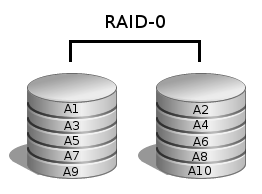
\includegraphics[width=.35\textwidth]{04/pics/raid-0}}
	\qquad
	\subfloat[Mirroring]{\label{fig:file-systems:raid-1}
			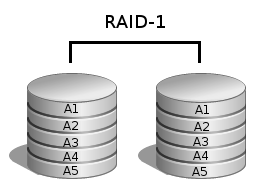
\includegraphics[width=.35\textwidth]{04/pics/raid-1}} \\
	\subfloat[Block-level striping with distributed parity]{\label{fig:file-systems:raid-5}
			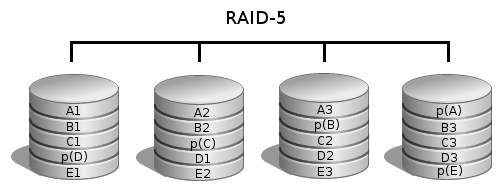
\includegraphics[width=.7\textwidth]{04/pics/raid-5}}
	\caption[RAID Levels illustrated]{Three of the most common RAID
		levels illustrated. RAID 0 increases performance, as blocks are
		written in parallel across all available disks. 
		RAID 1 provides redundancy, as blocks are written
		identically to all available disks.  RAID 5 aims to
		provide increased disk space as well as redundancy,
		as data is striped and parity information distributed
		across all disks.
		\label{fig:file-systems:raid}}
\end{figure}


\subsubsection{RAID 5}
\index{RAID!Level 5}

This level provides a bit of both RAID 0 and RAID 1:
data is written across all available disks, and for
each such stripe the data parity is recorded.  Unlike
in levels 2 through 4, this parity is not stored on a
single, dedicated parity drive, but instead
distributed across all disks.  See Figure
\ref{fig:file-systems:raid-5} for an illustration of
the block distribution.

Since parity information is written in addition to the
raw data, a RAID 5 cannot increase disk capacity as
linearly as a RAID 0.  However, any one of the drives
in this array can fail without impacting data
availability.  Again, as in the case of a RAID 1
configuration, the array will go into {\em degraded}
mode and get rebuilt when the failed disk has been
replaced.  However, the performance of the array is
decreased while a failed drive remains in the array,
as missing data has to be calculated from the parity;
the performance is similarly reduced as the array is
being rebuilt. Depending on the size of the disks
inquestion, this task can take hours; all the while
the array remains in degraded mode and another failed
drive would lead to data loss.

\subsubsection{Composite RAID and Failure Rates}

Since a RAID configuration creates a (virtual) disk to
present to the upper layer (such as the OS), it should
not come as a surprise that it is possible to combine
or nest RAID levels to achieve a combination of the
benefits provided by either one level; Table
\ref{table:file systems:raid-nested} lists some of the
most popular combinations.  In each case, we increase
fault tolerance at the expense of efficiency.

\begin{table}[b]
\centering
	\begin{tabular}{ l p{.75\textwidth}}
	\hline
	{\bf RAID 0+1} & Mirrored array of stripes \\
	{\bf RAID 1+0} & Striped array of mirrors \\
	{\bf RAID 5+0} & Striped array of multiple RAID 5 \\
	\hline
	\end{tabular}
	\caption{Standard RAID levels can be combined.}
	\label{table:file systems:raid-nested}
\end{table}

It is worth noting that the redundancy gained by
combining RAID levels is frequently overestimated.
Here's why: each drive has an expected failure rate,
each array a mean time to data loss.  The
``Independent'' in RAID misleads us to believe that
the odds of any one disk failing is entirely unrelated
to the others.  In reality, it is most common to use
identical drives from the same manufacturer if not
even the same production batch in a given array.  That
is, when a single drive fails and the array goes into
degraded mode, the probability of a second drive
failing is actually higher than one would expect with
truly independent drives.

Secondly, the actions performed by the RAID on the
disks needs to be taken into consideration as well.
When a disk in a RAID 5 array fails and is replaced,
{\em all} of the disks will undergo additional stress
as {\em all} of the data is read in order to rebuild
the redundant array.  This process may well take
several hours if not days -- a very long period of
time during which our data is at increased risk.  In
other words, the failure of a single drive will
necessarily increase the probability of failure of the
other drives\footnote{RAID 6 improves this situation,
at the expense of efficiency.  Dropping prices have
not very surprisingly lead more and more enterprise
environments to consider this trade-off entirely
acceptable.}.

When choosing a composite RAID architecture, it is
well worth our time to consider the Mean Time to
Recovery\index{Mean Time to Recovery} (MTTR) in
addition to the other factors.  From the moment that
a disk failure is detected until the array has been
rebuilt, our data is at severe risk.  In order to
reduce the MTTR, many system administrators deploy
so-called {\em hot spares}\index{hot
swapping}\index{RAID!Hot Spare}, disks that are
installed in the server and known to the RAID
controller, but that are inactive until a disk failure
is detected.  At that time, the array is immediately
rebuilt using this stand-by drive; when the faulty
disk has been replaced, the array is already in
non-degraded mode and the new disk becomes the hot
spare.

\begin{figure}[ht]
	\centering
	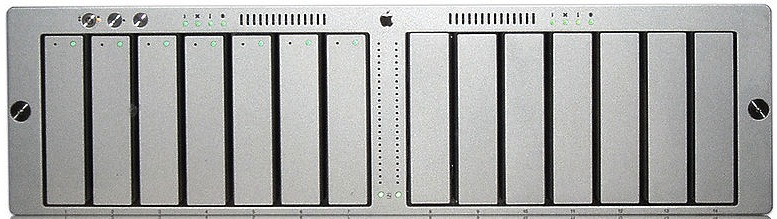
\includegraphics[width=.75\textwidth]{04/pics/xraid}
		\caption[Apple Xserve RAID]{An Apple Xserve RAID, a
			now discontinued storage device with 14 Ultra-ATA
			slots offering Fibre Channel connectivity and
			implementing a number of RAID levels in hardware
			as well as software across two independent
			controllers.
			\label{fig:file-systems:xraid}}
\end{figure}

\begin{figure}
\begin{experience}
{\bf Spectacular File System Confusion} \\

In early 2006, while working at Stevens Institute of
Technology as a System Administrator, we bought a new
Apple Xserve RAID storage device (like the one seen in
Figure \ref{fig:file-systems:xraid}) and populated its
14 disk slots with 400 GB drives, yielding (after
RAID, file system overhead and the previously
discussed discrepancy in binary versus decimal units)
two RAID5 configurations with a capacity of 2.2 TB
each, an impressive amount of affordable storage space
at the time. \\ [10pt]

The ``left'' RAID was dedicated to storing large
amounts of video and audio data made available to
clients running Mac OS X.  We connected the RAID
controller via Fibre Channel to a SAN switch, and from
there to an Apple Xserve network server, which managed
the HFS+ file system on this storage component. \\
[10pt]

The second 2.2 TB of storage space, the ''right'' side
of the array, was meant to become the central data
space for all workstations in the Computer Science and
Mathematics departments as well as their laboratories.
Up until then, this file space had been provided via
NFS from a two-module SGI Origin 200 server running
IRIX\index{IRIX}, managing a few internal SCSI disks as well
as some Fibre Channel direct attached storage.  We
intended to migrate the data onto the XServe RAID, and
to have it served via a Solaris 10 server, allowing us
to take advantage of several advanced features in the
fairly new ZFS and to retire the aging IRIX box.  \\
[10pt]

Neatly racked, I connected the second RAID controller
and the new Solaris server to the SAN switch, and then
proceeded to create a new ZFS file system.  I
connected the Fibre Channel storage from the IRIX
server and started to copy the data onto the new ZFS
file system.  As I was sitting in the server room, I
was able to see the XServe RAID; I noticed the lights
on the {\em left} side of the array indicate
significant disk activity, but I initially dismissed
this as not out of the ordinary.  But a few seconds
later, when the right side still did not show any I/O,
it dawned on me: the Solaris host was writing data
over the live file system instead of onto the new
disks!
\end{experience}
\end{figure}
% XXX remove pic?
\begin{figure}
\begin{experience}
\ContinuedFloat
I immediately stopped the data transfer and even
physically disconnected the Solaris server, but the
damage was done: I had inadvertently created a new ZFS
file system on the disks already containing (and
using) an HFS+ file system!  As it turns out, I had
not placed the Solaris server into the correct SAN
zone on the Fibre Channel switch, meaning the only
storage device it could see was the left side of the
array.  But since both sides of the array were
identical (in size, RAID type, manufacturer), it was
easy for me not to notice and proceed thinking that
due to proper SAN zoning, it was safe for me to write
to the device. \\ [10pt]

Now it was interesting to note that at the same time
as I was overwriting the live file system, data was
still being written to and read from the HFS+ file
system on the Apple server.  I was only able to
observe intermittent I/O errors.  Thinking I could
still save the data, I made my next big mistake: I
shut down the Apple server, hoping a clean boot and
file system check could correct what I still thought
was a minor problem.  \\ [10pt]

Unfortunately, however, when the server came back up,
it was unable to find a file system on the attached
RAID array!  It simply could not identify the device.
In retrospect, this is no surprise: the Solaris server
had constructed a new (and different) file system on
the device and destroyed all the HFS+ specific file
system meta data stored at the beginning of the disks.
That is, even though the blocks containing the data
were likely not over written, there was no way to
identify them.  After many hours of trying to recreate
the HFS+ meta data, I had to face the fact this was
simply impossible.  What was worse, I had neglected to
verify that backups for the server were done before
putting it into production use -- fatal mistake number
three!  The data was irrevocably lost; the only plus
side was that I had learned a lot about data recovery,
SAN zoning, ZFS, HFS+ and file systems in general.

\end{experience}
\end{figure}

\section{File Systems}
\label{sec:file systems}
\index{File Systems}

When the operating system is installed, it will create
a file system on the specified disk(s).  As we have
seen, these disks may be made available to the OS in a
variety of ways, but in the end, the OS does not
distinguish between a \gls{das} device such as a hard drive
disk, a volume created by an \gls{lvm}, a disk represented
by a RAID or one backed by a storage device over a
SAN.  This method of hiding hardware implementation
choices or details allows the OS to choose amongst a
number of different file systems, each with their own
unique strengths, disadvantages and performance
impacting tuning options.

Reduced to its most basic tasks, a file system is
responsible for storing, managing and updating data on
the storage device in question.  To this end, it needs
to manage the available space and be able to store
files as well as their attributes (i.e. {\em
metadata}) in a hierarchy that allows both the user
and the OS to efficiently retrieve them, as well as
ensure some level of file and file system integrity.
In addition, since Unix is a multi-user OS, the file
system depends on means to identify and distinguish
between different users; access control and the
concepts of {\em file permissions} are a basic
requirement.  What's more, Unix systems frequently
represent as ``files'' many things that us humans may
not usually think of as such\footnote{The ``Plan 9
from Bell Labs\index{Bell Laboratories}'' research
operating system\index{Plan 9} took the initial Unix
mantra of ``everything is a file'' much further: all
objects are either files or file systems,
communicating with each other via the {\em 9P}
protocol.  Network connections, communications with
the kernel's drivers, interprocess communication etc.
all are performed via standard I/O calls.}.  This
leads us to special purpose file systems that really
only provide a file I/O \gls{api} to their respective
resources: the {\em procfs}\index{procfs} file system,
representing information about the system's processes
and the {\em devfs}\index{devfs} file system, a
virtual file system acting as an interface to device
drivers are two examples.

\subsection{File System Types}
\label{file systems:types}

In this section, we will take a look at some of the
file systems commonly in use on Unix systems.  For the
most part, these are {\em disk file systems}, meaning
that they are designed to manage hard disk storage.
As we've seen in previous sections, the physical
layout of a hard drive influences partitioning
schemas, but the choice and creation of the operating
system's file system may also depend on the underlying
hardware.

As we discuss these file systems, we will find that
the approach to store both the actual file data as
well as the metadata, the information associated {\em
with} the files, differs significantly.  We will also
notice -- as a recurring pattern throughout this book
-- how different layers of abstraction help us improve
portability and provide a consistent interface, as
standard file I/O semantics can remain the same across
different file systems.

\subsubsection{Disk File Systems}
\index{File Systems!Disk}

A {\em Disk File System} is probably what most people
-- at least those who {\em would} think about these
kinds of things to begin with -- have in mind when they
think about what a file system does.  It manages block
device storage, stores ``files'' in ``directories'',
maintains a file system hierarchy, controls file
metadata, and allows for simple I/O via a few basic
system calls.  The canonical file system for the Unix
family of operating systems is, of course, the {\em
Unix File System} (\gls{ufs})\index{File Systems!UFS},
also known as the {\em Berkeley Fast File System}
(\gls{ffs})\index{Fast File System}.  We will look at
the UFS in detail in Section
\ref{sec:unix-file-system}, but for now suffice it to
say that this file system implementation and its use
of boot blocks, superblocks, cylinder groups,
{\em inodes}\index{inode} and data blocks is repeated and
reflected in many other Unix file systems, including
for example {\em ext2}\index{File Systems!ext2}, for a
long time the default file system for Linux systems.

These traditional file systems suffer a notable
drawback in the case of unexpected power failure or a
system crash: some of the data may not have been
committed to the disk yet, causing a file system
inconsistency.  When the OS boots up again, it will
need to perform time consuming checks (see
\manpage{fsck(8)}) and any problems found may not
actually be recoverable, leading to possible data
loss.  In order to address these problems, a so-called
{\em journaled} file system might choose to first
write the changes it is about to make to a specific
location (the journal) before applying them.  In the
event of a crash, the system can then simply replay
the journal, yielding a consistent file system in a
fraction of the time it would take a traditional file
system to traverse the entire hierarchy to ensure
consistency.

There are many different journaled file systems,
including a number of commercial implementations (such
as Apple's {\em HFS+}\index{File Systems!HFS+}, IBM's
{\em JFS}\index{File Systems!JFS}, or SGI's {\em
XFS}\index{File Systems!XFS}) and open source variants
(including {\em ext3}, {\em ext4}\index{File
Systems!ext3}\index{File Systems!ext4} and {\em
reiserfs}\index{File Systems!reiserfs} for Linux and
updates to UFS/FFS providing support for journaling or
logging).

Despite the differences in how data is ultimately
written to the disk, the fundamental concepts of how
data and metadata are managed, the use of the {\em
inode} structures, or the {\em Virtual File System}
layer to allow the kernel to support multiple
different file systems remains largely the same across
the different Unix operating and file systems.

\subsubsection{Distributed File Systems}
\index{File Systems!Distributed}

Unlike a disk file system, which provides access to
the data it holds only to the processes running in the
operating system the disk is attached to, a {\em
distributed file system} may allow different client
systems to access a centralized storage resource
simultaneously, thus forming the basis for any
\gls{nas} solutions.  As we discussed in Section
\ref{file systems:storage-models:nas}, this model
implies that clients no longer operate on the block
level of the storage -- this access has been
abstracted on a higher level and the client OS thus
requires in-kernel support for the file system in
question.

Sun Microsystems\index{Sun Microsystems}' {\em Network
File System} (\gls{nfs})\index{File Systems!NFS},
created in 1985, was the first such file system
utilizing the {\em Remote Procedure
Calls}\index{Remote Procedure Calls} (RPC) via the
Internet Protocol (IP)\glslink{ip}\index{Internet
Protocol} for the server to communicate with the
clients, and remains to this day the standard
distributed file system in the Unix world.  Other
notable variations include the {\em Andrew File
System} (\glslink{afs}{AFS})\index{File Systems!Andrew
File System/AFS} and its descendent, {\em Coda},
developed at Carnegie Mellon University\index{Carnegie
Mellon University}, tightly integrated with the
Kerberos\index{Kerberos} authentication protocol, and
backed by a local cache, making it particularly
tolerant of network interruptions, as well as the {\em
Server Message Block}/{\em Common Internet File
System} ({\em
\glslink{smb}{SMB}/\glslink{cifs}{CIFS}}), the
predominant network file system in the Windows world,
made accessible to Unix systems via the
``Samba''\index{Samba} implementation of these
protocols.

Within the area of massive scale Internet systems, a
number of specialized, distributed file systems have
emerged, most notably the {\em Google File
System}\cite{filesystems:gfs}\index{File
Systems!Google/GFS} and the {\em Hadoop Distributed
File System}\cite{filesystems:hdfs}\index{File
Systems!Hadoop/HDFS} (the latter being an open source
implementation modeled after the former).  These file
systems provide highly scalable fault tolerance while
at the same time providing high performance on
low-cost commodity hardware.

As usual, different problems call for different
solutions, and despite their significant capabilities,
these file systems may not necessarily be suitable for
your requirements.  In fact, making use of these
capabilities requires a significant investment -- both
in the time and expertise required to manage them as
well as in the hardware required to really get
anything out of them.

Other distributed file systems may have a different
focus, leading to interesting and entirely distinct
properties: the {\em Tahoe Least-Authority File
System}\cite{filesystems:tahoe-lafs}\index{File
Systems!Tahoe Least-Authority}, for example, provides
data confidentiality through the use of cryptography,
thus allowing complete decentralization over the
(public) Internet.  On the other hand, the advent of
cloud computing has further blurred the boundaries of
where a distributed file system ends and where a
network service begins: Amazon's {\em Simple Storage
Service} (\glslink{s3}{S3})\index{AWS!S3}, for
example, despite being an \gls{api} driven web
service, might as well be considered a distributed
file system, but then so could online storage
providers, such as Dropbox, who build their
solutions on top of Amazon's service.  It will be
interesting to see how these distributed file systems
or data stores evolve with time.


\subsubsection{``Other'' File Systems}
\index{File Systems!Special Purpose}

In the Unix world, there exists an old mantra:
``Everything is a file.'' That is, the simple
\gls{api} defining file I/O has proven so useful that
a number of non-file ``things'' have come to implement
this interface as well: not only can regular files be
accessed using the \manpage{open(2)},
\manpage{read(2)}, \manpage{ write(2)} and
\manpage{close(2)} system calls\footnote{All of these
system calls operate on a small non-negative integer,
the so-called file {\em descriptor} or file {\em
handle}.  The old expression should therefore more
accurately be cited as ``Everything is a file
descriptor.''}, but so can network sockets and other
interprocess communication endpoints, character and
block devices, so-called {\em pseudo-devices} (such as
{\tt /dev/null}\index{\tt /dev/null}), and various
other ``special files''.

Similarly, a number of pseudo- and virtual file
systems have been created to use the same \gls{api}
and make resources available using file-like
structures.  The access points for these structures
becomes a mount point in the file system hierarchy,
{\em et voil\`{a}}, these resources can be accessed,
processed and manipulated using common Unix tools.
Examples include the {\em devfs}\index{File
Systems!Device} virtual file system (used to access
special and general devices), the {\em procfs} pseudo
file system (providing information about system
information and individual processes), the {\em
UnionFS}\index{File Systems!Union} (a method of
layering two regular file systems on top of each
other, providing the union of the two hierarchies to
the user), and {\em tmpfs}\index{File
Systems!Temporary} (a method of creating a file system
in virtual memory, granting significant performance
benefits).

In addition to these cases, there are also a number of
file systems that have been created to meet very
specific requirements, or that effectively function as
an overlay on top of an application or protocol in
order to facilitate local file access to remote
resources, such as, for example, the SSH file system.
But file systems are usually implemented in the
operating system's kernel space: file I/O system calls
do happen here and devices and certain other resources
can only be controlled by the kernel; likewise,
mounting or unmounting file systems requires superuser
privileges.  But not all file systems are actually
accessing any of the resources protected by the
kernel.  In order to facilitate non-privileged access
to file system interfaces, some Unix systems have
created kernel modules that provide a method to
implement virtual ``File Systems in
Userspace''\index{File Systems!Userspace/Fuse} (known
as {\em FUSE}).

All of these file systems that aren't actually {\em
file} systems but rather an abstraction of other
resources into a file \gls{api} illustrate how much the
concept of simplicity permeates the Unix culture.  At
this point, few system administrators would wish to
part with the convenience of, for example, {\em
procfs} -- in fact, its availability is almost
universally assumed.  For a polyglot administrator,
however, it is important to be familiar with the
different pseudo- and virtual file systems available
on the different Unix versions and, more importantly,
know how to access the resources they represent in
their absence.

\section{File System Layout}
\label{file systems:layout}

The traditional Unix file system layout is organized
as a tree-like hierarchy, rooted at {\tt /}
(``slash'').  Under this directory reside a number of
standard top-level subdirectories, each with a
well-defined purpose and containing further
subdirectories, forming a hierarchy described in the
{\tt hier(7)}\index{\tt hier(7)} manual page.

Unix systems can make use of multiple different file
systems on multiple partitions at the same time.  Each
may be attached or ``mounted'' under any directory (or
``mount point'') of the file system hierarchy with the
exception of the root file system: the file system
containing the basic operating system and from which
the system was booted, which must be mounted at {\tt
/}.

Figure \ref{fig:file-systems:layout} illustrates a
subtree of the typical Unix hierarchy with different
components residing on separate disks.  Each node in
the tree represents a directory entry used to map
file names to inodes\index{inode}; nodes with children
represent directories, leaf nodes represent regular
files.  Traversing the tree from the root to any given
node constructs a so-called
``pathname\index{pathname}'' consisting of directory
names concatenated with a path separator, ``{\tt /}'',
followed by the file name.

\begin{figure}[ht]
	\centering
	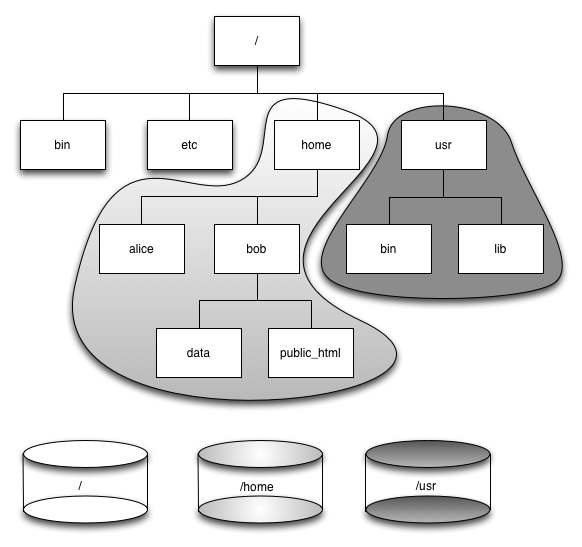
\includegraphics[width=.75\textwidth]{04/pics/filesystem-tree-mountpoints}
		\caption[File System Hierarchy]{The Unix file system is a
			tree-like structure, rooted at {\tt /}; 
			different file systems can be attached at
			different directories or mount points.  In
                        this illustration, {\tt /home} and {\tt /usr}
                        reside on separate disks from {\tt /}.
			\label{fig:file-systems:layout}}
\end{figure}


File names may contain any character except for this
separator or the {\em NUL} character ({\tt
\textbackslash0}), used in the the C programming
language to terminate a string.\footnote{It is a
common mistake to assume that a file name contains
only printable characters.  The Unix system does not
impose many restrictions on how a user might choose
to name a file, and file names containing e.g. control
characters such as a carriage return (``{\tt \\n}''),
while confusing on a line-buffered terminal, are
possible.}  Most Unix systems impose a maximum file
name length of 255 bytes and a maximum pathname length
of 1024 bytes; however, these are file system and OS
specific limits.

Every Unix process has the concept of a current
working directory -- run the \manpage{pwd(1)} command
or type ``{\tt echo \$PWD}'' in your shell to display
where in the file system hierarchy you currently are.
Pathnames may either be {\em relative} to this
location, or, if they begin with a {\tt /}, {\em
absolute}.

Each directory contains at least two entries: ``{\tt
.}'' (dot), a name for the current working directory
and ``{\tt ..}'' (dot-dot), a name for the parent
directory.\footnote{As a special case, within the root
directory both ``{\tt .}'' and ``{\tt ..}'' refer to
the same directory, i.e. {\tt /}.}  Since relative
pathnames are resolved from within the current working
directory, the same file can be referred to by
different names, as shown in the examples in Listing
\ref{code:pwd}.

\begin{lstlisting}[float,basicstyle=\scriptsize,label=code:pwd,caption={[Absolute
and relative pathnames] Absolute pathnames begin with
a {\tt /} and are resolved from the root of the file
system; relative pathnames are resolved from the
current working directory.}]
$ pwd
/home/jschauma              # pwd(1) writes the absolute pathname
$ echo hello > file         # create "file" in the current directory
$ cd /usr/share/doc         # cd(1) using an absolute pathname
$ pwd
/usr/share/doc              # no surprise here
$ cat /home/jschauma/file   # now using an absolute pathname
hello
$ cd ../../../home/jschauma # cd(1) using a relative pathname
$ pwd
/home/jschauma
$ cat file                  # "./file" would also work
hello
$ 
\end{lstlisting}

\section{The Unix File System}
\label{sec:unix-file-system}
\index{File Systems!Unix}\index{Unix File System}\index{UFS}\index{FFS}

As we discuss the general concepts of file systems in
the Unix world, it is impossible to avoid a much
closer look at the {\em \acrlong{ufs}} (\gls{ufs}),
the initial standard file system for a
number of both commercial and open source Unix
versions for decades.  UFS, also known as the {\em
Berkeley Fast File System} or \gls{ffs}, created by
Marshall Kirk
McKusick\cite{filesystems:ffs}\index[names]{McKusick,
Marshall Kirk} and others at the University of
California in Berkeley in 1984, was a reimplementation
of the original file system provided by Bell
Lab\index{Bell Laboratories}'s UNIX\index{UNIX} V7.

\begin{figure}[t]
	\centering
	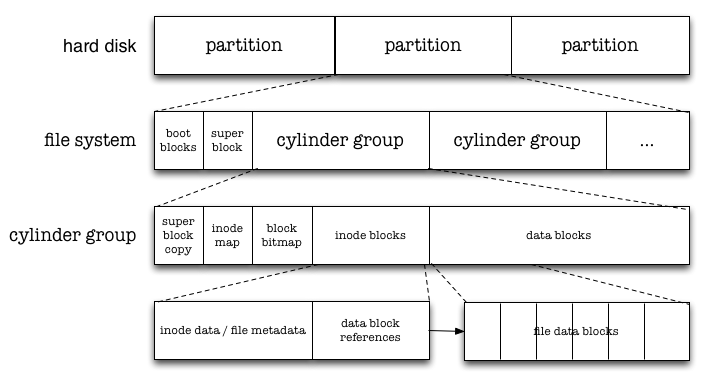
\includegraphics[width=.85\textwidth]{04/pics/ufs-details}
		\caption[UFS Details]{A disk may be divided into multiple
			partitions; a partition may contain a file system
			with multiple cylinder groups; each cylinder group
			contains some file system meta data as well as
			inode and data blocks.
			\label{fig:file-systems:ufs-details}}
\end{figure}

These improvements and changes introduced most notably
the concept of cylinder groups, providing a more equal
distribution of the file metadata on the physical
disk, thus minimizing seek time.  The Unix File System
therefore consisted of the following major components,
as illustrated in Figure
\ref{fig:file-systems:ufs-details}:

\begin{itemize}
	\item A {\bf superblock}\index{superblock}.  This block contains all the
		system's crucial information, such as the number and
		location of cylinder groups used as well as the location of the
		inode and data blocks.  As this information is critical for
		the operation of the file system and corruption of this
		block would be disastrous, it is replicated and stored in
		a number of (predictable) locations.  This allows
		the super user to repair a corrupted file system by pointing to an
		alternate superblock.
	\item A number of {\bf cylinder groups}\index{cylinder groups}, which break the large
		file system into more manageable chunks by distributing
		meta data evenly across the physical partition.
	\item A number of {\bf inode maps} (one for every cylinder group),
		pointing to the cylinder group's {\bf inode blocks}, which
		in turn contain the metadata associated with the files.
	\item A number of {\bf block bitmaps} (one for every cylinder
		group), pointing to the cylinder group's {\bf data blocks},
		which in turn contain the actual file data.
\end{itemize}

The distribution of this data across multiple cylinder
groups illustrates the tight relationship that the
file system had with the physical properties of a hard
disk drive; this layout remains in place nowadays,
even though on solid state drives, for example, we no
longer suffer performance penalties due to seek time.

It is important to note that the data blocks used by
the file system are different from the {\em physical}
blocks of the hard disk.  The latter are, as we
discussed in Section
\ref{sec:file-systems:physical-disk-structure}, 512
bytes in size (or, in more recent drives, 4096 bytes);
the former -- called the {\em logical} block size --
can be decided on by the system administrator at file
system creation time.  UFS uses a minimum logical
block size of 4096 bytes, and defaults to larger block
sizes based on the overall size of the file system.
Likewise, the number of inodes in a file system is
fixed once the file system has been created.  Here,
UFS defaults to an {\em inode density} of one inode
per 2048 bytes of space for small file systems --
consult the \manpage{newfs(8)} manual
page for this and other parameters to define and tune
the file system at its creation time. \\


Let us dive a little bit deeper and think about how
the Unix File System manages disk space:  A file
system's primary task is to store data on behalf of
the users.  In order to read or write this data, it
needs to know in which logical blocks it is located.
That is, the file system needs a map of the blocks, a
way to identify and address each location.  This is
accomplished by way of the {\em inode} and {\em data
block} maps: the total number of inodes represents the
total number of files that can be referenced on this file
system, while the data blocks represent the space in
which the file data is stored.

As we noted, a data block is, necessarily, of a fixed
size.  That means that if we wish to store a file that
is larger than a single block, we have to allocate
multiple blocks and make a note of which blocks
belong to the given file.  This information is stored
as pointers to the disk blocks within the
inode\index{inode} data structure.

Unfortunately, however, not all files will be
multiples of the logical block size.  Likewise, it is
possible that files will be smaller than a single
block.  In other words, we will always end up with
blocks that are only partially allocated, a waste of
disk space.  In order to allow more efficient
management of small files, UFS allowed a logical block
to be divided further into so-called {\em fragments},
providing for a way to let the file system address
smaller units of storage.  The smallest possible
fragment size then is the physical block size of the
disk, and logical blocks are only fragmented when
needed.

A pointer to the data blocks and fragments allocated
to a given file is stored in the inode data structure,
which comprises all additional information about the
file.  This allows for an elegant separation of a
file's metadata, which takes up only a fixed and small
amount of disk space, and its contents.  Accessing the
metadata is therefore independent of the file size
(itself a piece of metadata), allowing for efficient
and fast retrieval of the file's properties without
requiring access of the disk blocks.  Other pieces of
information stored in the inode data structure include
the file's permissions, the numeric user-id of the
owner, the numeric group-id of the owner, the file's
last access, modification and file status change
times\footnote{A file's {\tt ctime}, it's time of last
file status change, is frequently misinterpreted to be
the file's {\em creation} time; most file systems,
including UFS, do {\em not} store this kind of
information.  Instead, the {\tt ctime} reflects the
last time the meta information of a file was
changed.}, the number of blocks allocated for the
file, the block size of the file system and the device
the file resides on, and of course the inode number
identifying the data structure.

% XXX: formatting/wrapping?
\begin{lstlisting}[float,basicstyle=\scriptsize,label=code:ls-ai,caption={[Output
of {\tt ls -ai}]Use of the ls(1) command on a NetBSD
system to illustrate how file names are mapped to
inode numbers in a directory.  (Note that in the root
directory both '.' and '..' have the same inode
number\, as in this special case they actually are the
same directory.)}]

$ ls -ai /
      2 .         5740416 cdrom    5816448 libexec  2775168 stand
      2 ..        1558656 dev      1862784 mnt      2166912 tmp
3003280 .cshrc     988439 emul           4 netbsd   3573504 usr
3003284 .profile   342144 etc      1824768 proc     3497472 var
3421440 altroot   1026432 home      798336 rescue
5702400 bin       3763584 lib      3003264 root
      3 boot.cfg  2204928 libdata  5588352 sbin
$
\end{lstlisting}

Now humans tend to be rather bad at remembering large
numbers and prefer the use of strings to represent a
file, but the one piece of information that is {\em
not} stored in the inode is the file name.  Instead,
the Unix File System allows for a mapping between a
file name and its unique identifier -- its inode --
through the use of directories.  A directory really is
nothing but a special type of file: it has the same
properties as any other file, but the data it holds is
well-structured (in contrast to the byte stream
contained in so-called ``regular'' files) and consists
of inode number and file name pairs.  You can use the
\manpage{ls(1)} command to illustrate this --
see Listing \ref{code:ls-ai}.

A mapping of an inode number to a file name is called
a {\em hardlink}\index{link!hard}, even though humans
tend to prefer the term ``file name''. An inode can be
accessed by more than just one file name: within a
single file system, each file may be referenced by
multiple names in different directories, and the
number of hardlinks for a given file is stored in the
inode data structure as well.  But since each file is
identified by its inode number, and since multiple
file systems can be mounted in a running operating
system, it is possible that two files on two different
file systems have the same inode number.  As a result,
a file is really only uniquely identified by its
combination of file system device and inode number.
What's more, at times it may be useful to create a
pointer to a file residing on a different file system,
but as just explained, creating a hard link across
file system boundaries is impossible.  To overcome
this limitation, so-called ``symbolic
links''\index{link!symbolic} were invented: a symbolic
link (often abbreviated as ``symlink'') is a special
kind of file that contains as its only contents the
path name of the file it references.  Almost all
operations on a symlink will then be redirected to the
target file it points to.

In addition to regular files (hard links), directories
and symbolic links, the following file types are
supported by the traditional Unix file system:

\begin{itemize}
	\item {\em Block special devices} -- an interface for disk-like
		devices, providing buffered and non-sequential I/O.
	\item {\em Character special devices} -- an interface for
		communication devices such as keyboards, mice, modems, or
		terminals, providing unbuffered I/O.  A number of virtual,
		so-called pseudo-devices such as {\tt /dev/null}\index{\tt /dev/null}, {\tt
		/dev/zero}\index{\tt /dev/zero},  or {\tt /dev/urandom}\index{\tt /dev/urandom}, for
		example, are also accessed as character special devices.
	\item Named pipes or {\em FIFO}s -- another inter-process
		communications endpoint\index{IPC!FIFO} in the file
		system.  This type of file represents a manifestation of
		the traditional Unix pipe in the file system name space;
		I/O is performed using the same methods as for any regular
		file.  As data is merely passed between processes, a FIFO
		always has a file size of zero bytes.
	\item Unix domain {\em sockets} -- an inter-process communications
		endpoint\index{IPC!Unix domain socket} in the file system
		allowing multiple processes with no shared ancestor
		process to exchange information.  Communication happens
		via the same \gls{api} as is used for network sockets.
\end{itemize}

\begin{lstlisting}[float,label=code:stat,caption={[Output of {\tt stat(1)}]Sample
output of the stat(1) command on a Linux system\, showing the various pieces of
information stored in the inode data structure for the file ``/etc/passwd''.}]
$ stat /etc/passwd
  File: `/etc/passwd'
  Size: 2062      	Blocks: 8       IO Block: 4096   regular file
Device: ca02h/51714d	Inode: 725181   Links: 1
Access: (0644/-rw-r--r--)  Uid: (0/root)   Gid: (0/root)
Access: 2011-08-26 23:45:31.000000000 -0400
Modify: 2011-08-26 23:45:31.000000000 -0400
Change: 2011-08-26 23:45:31.000000000 -0400
$
\end{lstlisting}

The file type as well as its permissions and all the
other properties of a file can be inspected using the
\manpage{stat(1)} command (see Listing \ref{code:stat}
for an example), or, perhaps more commonly, using the
\manpage{ls(1)} command (as illustrated in Figure
\ref{fig:file-systems:ls-l}).  This command is so
frequently used and its output so ubiquitous that any
system administrator can recite the meaning of the
fields in their sleep.  The semantics and order in
which permissions are applied, however, include a few
non-obvious caveats, which is why we will look at the
Unix permissions model in more detail in Chapter
\ref{chap:multi-user}. \\

Over the last 30 years, UFS has served as the
canonical file system for almost all Unix versions.
With time, a number of changes have become necessary:
more fine-grained access controls than the traditional
Unix permissions model allows were made possible via
file system extensions such as
\gls{acl}s\index{Access Control Lists}; larger storage
devices required not only updates to the block
addressing schemas, but also to the different data
types representing various file system aspects;
today's huge amounts of available data storage have
made log-based file systems or journaling capabilities
a necessity, and massively distributed data stores
pose entirely different requirements on the underlying
implementation of how the space is managed.

Yet through all this, as enhancements have been made
both by commercial vendors as well as by various open
source projects, the principles, the very fundamentals
of the Unix File System have remained the same:  the
general concept of the inode data structure and the
separation of file metadata from the data blocks have
proven reliable and elegant in their simplicity.  At
the same time, this simplicity has proven to yield
scalability and adaptability: the persistent idea that
``everything is a file'', and that files simply
store bytes and thus have no inherent structure
(unlike a database or certain archives) have allowed a
surprising flexibility and lead to the creation of
many pseudo- or virtual file systems providing a
simple \gls{api} and User Interface (UI) to any number
of resources.

\begin{figure}[t]
	\centering
	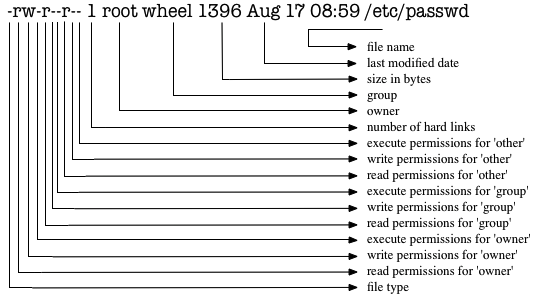
\includegraphics[width=.75\textwidth]{04/pics/ls-l}
		\caption[File Metadata]{The default output of the {\tt ls -l}
			command includes most of the metadata of a given
			file.
			\label{fig:file-systems:ls-l}}
\end{figure}

\section{Conclusions}
\label{file systems:conclusions}

Throughout this chapter, we have built our
understanding of file systems and storage models from
the ground up.  We have seen how simple concepts are
combined to construct increasingly complex systems --
a pattern that weaves like a red thread through all
areas we cover.  We noted the circular nature of
technology development: the simple \gls{das} model
repeats itself, albeit more complex and with
additional layers, in common SANs, much as network
attached storage utilizes both DAS and SAN solutions,
yet is taken to another extreme in cloud storage
solutions.

Being aware of the physical disk structure helps us
understand a file system's structure: we realize, for
example, that concentric cylinder groups make up
partitions, and that the location of data blocks
within these cylinders may have an impact on I/O
performance.  What's more, the concepts of file system
blocks become clearer the further we deepen our
knowledge of both the logical and physical components,
and the distinction of metadata from the actual
contents of a file allow us to explain how the various
file system related Unix tools operate on a fairly low
level as well as how to tune these values at file
system creation time.  As system administrators, this
understanding is crucial.

But what about our earlier point of noting the three
pillars of strong system architecture and design:
Scalability, Security, Simplicity.  What role do these
play in the context of file systems and storage
models? \\

Scalability is defined by our aptitude to meet
changing requirements.  As far as file systems are
concerned, we need to be able to provide sufficient
storage that meets our performance and rapidly
increasing space requirements.  One might be tempted
to jump to a quick conclusion and choose the
superficially ``most flexible'' solution, which
nowadays often appears to be a cloud based storage
model.  However, it behooves us to take a step back
and consider the other two major design decisions,
simplicity and security, which help us cut through
complexities and clarify just how flexible such a
model might be.  Reliance on a third party provider
for data storage, for example, incurs a number of
hidden costs: bandwidth requirements increase, data
redundancy and duplication need to be weighed, backup
and data migration strategies change radically, and
vendor lock-in may in fact eliminate true
flexibility.\footnote{Depending on the size of your
organization, these costs may in fact not be hidden
at all: at some point, you may find yourself providing
``cloud storage'' to your organization, and all of a
sudden you are the owner of that infrastructure.}.

So what makes for a scalable storage solution?  On the
one hand, we need to be able to add disk space on
demand, so we either require a file system that can
grow as needed, or an efficient way to synchronize
multiple file systems.  This already illustrates a
trade-off in complexity and the solutions depend in
part on our network architecture:  within a single
system, the use of an \gls{lvm} or a file system that
allows the pooling of multiple resources seems a good
choice, but how do you make that available to multiple
clients?  If you have hosts in distinct geographical
locations, connected only via the Internet (an
inherently untrustworthy network), how do you allow
for shared access?

The more you think about these requirements, the more
you will find yourself weighing conflicting
approaches.  You will go back and forth between the
simplest possible solution (for example, all hosts
write data only to direct attached storage) and the
more complex (shared storage available via a
distributed file system or a cloud architecture).  But
it becomes increasingly hard to define ``simple'', as
each solution requires considerations outside of the
initial problem domain: hosts writing to \gls{das} is
efficient, but data synchronization across all hosts
becomes increasingly complicated; a shared storage
pool available over the network solves that problem,
but incurs a high cost of complexity and dependency on
the supporting infrastructure.

What's more, the security aspects of the file system
and the features it provides are manifold:  as Unix
was designed from the beginning as a multi-user
operating system, the capabilities to distinguish
between different users were built into the system and
is reflected in the file permissions.  But file system
security goes beyond this basic level, especially when
we consider access over the network.  Every
distributed file system has to solve the problem of
deciding whether or not a remote system should be
granted access to a given resource, and how such a
system should authenticate.  The access models range
from simplistic (if you are on the local network, you
are granted access) to the more sophisticated (a
client has to present some sort of time-limited
authentication token to gain access).

But a system administrator's professional paranoia
dictates digging {\em even} deeper.  In the case of
distributed file systems, of storage area networks or
of remotely hosted, cloud-based storage solutions, we
not only have to consider how a remote client
authenticates and is granted access, but also who has
access to the bits and bytes in transit, or how to
protect our data's confidentiality should a remote
system be compromised.  Is transport security assumed,
or do we rely on secure network connections (for
example on the network layer via a VPN or
IPsec\index{IPsec} tunnels, or on the application
layer via \glslink{tls}\index{TLS} or
SSH\index{SSH}, to name but a few examples)?  Is data
stored ``in the cloud'' accessible to anybody with
access to the physical device (simple, but trust is
placed into the storage provider, often a third
party), or do we encrypt it (more secure, but also
more complex)?  Under what jurisdiction is the data
stored, and what data could be subpoenaed by which
authorities?\index{government access}  Would you even
be notified if access to your and your users' data was
granted to law enforcement\index{law enforcement}? \\

As we will see throughout this book, there never is a
single solution to all our problems.  We will
continually have to make trade-offs based on
assumptions and probabilities, usability
considerations and practical concerns.  There is no
silver bullet, no one solution, no unique, always
correct approach.  This is why it is so important for
a system administrator to be aware of {\em all} the
factors, and to ask the questions we've started to
suggest here at the end of this chapter.  Not
surprisingly, this line of questions quickly leads us
beyond the basic concepts of file systems and storage
models, but likewise often brings us full circle when
we have to consider higher level applications and
consider just how exactly they access data and what
kinds of assumptions and requirements they pose as to
availability, security and performance.  The topics
covered in this chapter are the foundation upon which
our systems are built.

\vfill
\pagebreak

\chapter*{Problems and Exercises}
\addcontentsline{toc}{chapter}{Problems and Exercises}
\section*{Problems}
\addcontentsline{toc}{section}{Problems}

\begin{enumerate}

\item
Identify the storage area model(s) predominantly used in your
environment(s).  What kind of problems with each do you frequently
encounter?  Would changing the storage model be a feasible solution to
these problems?  Why or why not?

\item
Research the implementation details of a popular cloud storage provider.
What storage solutions did they choose?  Can you identify all the
different models we discussed?

\item
Identify at least three distinct security concerns in each of the storage
models we discussed.  Outline in detail how an attacker might exploit such
weaknesses and how a System Administrator might prevent or counter each
attack.

\item
\label{prob:disks:hdds}
Ask your system administrators if they have any old or broken hard drives,
if possible from different manufacturers or with different capacities.
Open up the drives and identify the various components.  How many
read-write heads are there?  How many platters?  How do the different
models differ?

\item
\label{prob:disks:disklabel}
Compare the output of the \manpage{fdisk(8)} command on different operating
systems.  Divide a disk into a number of different partitions, then use
\manpage{disklabel(8)} to review the resulting label.  Identify all the
different partitions, verify their capacities and explain any
discrepancies or unexpected findings.

\item
Compare the various composite RAID levels and analyze their respective
fault tolerance and mean time to recovery in the case of one or more
failed disks.

\item
Assuming 500 GB disk drives, what is the total capacity of a RAID
configuration using 7 disks under RAID 0, RAID 1, RAID 5, RAID 6, RAID
0+1, RAID 1+0 and RAID 5+0?

\item
You want to create a RAID 5 using several multi-terabyte
drives.  Research and choose your preferred hardware,
paying particular attention to their {\em
Unrecoverable Read Error}\index{Unrecoverable Read
Error} rates (i.e. the mean time to failure, usually
expressed as number of bits read).  If the array is
filled to capacity with data, and one of the drives
failes and has to be replaced, how much data do you
end up reading when you rebuild the array?  What does
this say about the probability of an additional disk
failure while you're still in degraded mode?

\item
Identify the different file systems in use on the Unix
versions you have access to.  How many partitions are
there, where are they mounted, what mount options do
they use?  Were they chosen explicitly or do they
appear to be OS defaults?

\item
Identify all resources made available by the {\em procfs} system, both
about the system and about individual processes.  Suppose {\em procfs} was
not available, how would you go about finding out the same information?

\item
Identify the different devices found under {\tt /dev}.  What is the
difference between {\tt /dev/null} and {\tt /dev/zero}, between {\tt
/dev/random} and {\tt /dev/urandom}?

\item
Identify the file system limitations on a system you have access to.  What
is the maximum file system size?  What is the maximum file size?  What
characters may be used in a file name?  How many files can you create in a
single directory?

\item
Compare at least four different file systems with respect to their default
block size and inode density.  Consider both small (less than 1 GB in
size), ``normal'', and very large (more than 1 TB in size) partitions or
volumes.  How efficiently does each system manage this space?  Can you
specify different inode and block sizes to increase efficiency?

\item
Review the concepts of inode mappings to file names, hard links, and
symbolic links.

\begin{enumerate}

\item
Create a new file, then create a second hard link for this file.  Verify
that both files are completely identical by using {\tt ls(1)}, {\tt
stat(1)} and by appending data to one of the files and reading from the
other.

\item
Rename the original file and repeat -- what changed?  Why?

\item
Create a new file, then create a symbolic link for this file.  Verify that
both the original file and the symbolic link are unique by inspecting
their inode numbers.  Then append data to the file using the regular name
and confirm that reading from the symbolic link yields the same data.

\item
Rename the original file and repeat -- what changed?  Why?
\end{enumerate}

\item

Create a very large file.  Measure how long it takes
to rename the file within one directory using the {\tt
mv(1)} command.  Next, use {\tt mv(1)} to move the
file into a directory on a different file system or
partition.  What do you observe?  Explain the
difference.

\item
Experiment with the usability, resilience and
limitations of a system's root file system.

\begin{enumerate}

\item
Identify how much free disk space you have, then fill
it up.  Can you use up all available space using a
single file?  What are the effects of using up all
disk space?  Can you still create new, empty files?
Can you still log in?  Why/why not?

\item
Identify how many free inodes are available on your
root file system, then use them up by, e.g., creating
lots and lots of empty files.  What happens to the
directory size in which you create these files?  What
is the error message once you run out of inodes?  Can
you still create new files?  Can you still write to
existing files?  How much disk space is available now?
Can you still log in?  Why/why not?

\end{enumerate}


\end{enumerate}

\pagebreak

\bibliographystyle{plainnat}
\begin{thebibliography}{99}

\bibitem{disks:emc2-storage} EMC Education Service,
{\em Information Storage and Management: Storing, Managing, and Protecting
Digital Information}, John Wiley \& Sons, 2009

\bibitem{disks:frisch} \AE leen Frisch, {\em Essential System
Administration}, O'Reilly Media, 2002

\bibitem{filesystems:gfs} Sanjay Ghemawat, Howard Gobioff, and Shun-Tak
Leung, {\em The Google File System}, in ``Proceedings of the nineteenth
ACM symposium on Operating systems principles'', 2003, ACM, New York, NY;
also available on the Internet at
{\url http://research.google.com/archive/gfs-sosp2003.pdf}
(visited September 6th, 2012)

\bibitem{filesystems:hdfs} {\em The Hadoop Distributed File System:
Architecture and Design}, on the Internet at
{\url https://hadoop.apache.org/common/docs/r0.14.4/hdfs\_design.html}
(visited September 6th, 2012)

\bibitem{filesystems:tahoe-lafs} Zooko Wilcox-O'Hearn, Brian Warner, {\em
Tahoe -- The Least-Authority Filesystem}, in ``Proceedings of the 4th ACM
international workshop on Storage security and survivability'', 2008, ACM,
New York, NY; also available on the Internet at
{\url http://tahoe-lafs.org/\~{}zooko/lafs.pdf}
(visited September 6th, 2012)

\bibitem{filesystems:esr-taoup}Eric Steven Raymond, {\em The Art of Unix
Programming}, Addison-Wesley Professional, September 2003; also available
on the Internet at
{\url http://catb.org/\~{}esr/writings/taoup/}
(visited January 7, 2012)

\bibitem{filesystems:apue}W. Richard Stevens, Stephen A. Rago, {\em
Advanced Programming in the UNIX Environment}, Addison-Wesley
Professional; 2nd edition, 2005

\bibitem{filesystems:silberschatz}Abram Silberschatz, Greg Gagne, Peter B.
Galvin {\em Operating System Concepts}, John Wiley \& Sons, 2011

\bibitem{filesystems:ffs}Marshall Kirk McKusick, William N. Joy, Samuel J.
Leffler and Robert S. Fabry {\em A Fast File System for UNIX}, 
ACM Transactions on Computer Systems 2 (3), 1984, ACM, New York, NY; also
available on the Internet at
{\url http://www.cs.berkeley.edu/\~{}brewer/cs262/FFS.pdf} (visited September
9, 2012)

\end{thebibliography}

\chapter{Software Installation and Package Management}
\label{chap:software-installation}

\begin{quote}
{\em There is no neat distinction between operating system software
and the software that runs on top of it.} --
Jim Allchin\index[names]{Allchin, Jim}
\end{quote}

% XXX better graphic
\begin{figure}[hb]
	\raggedleft
	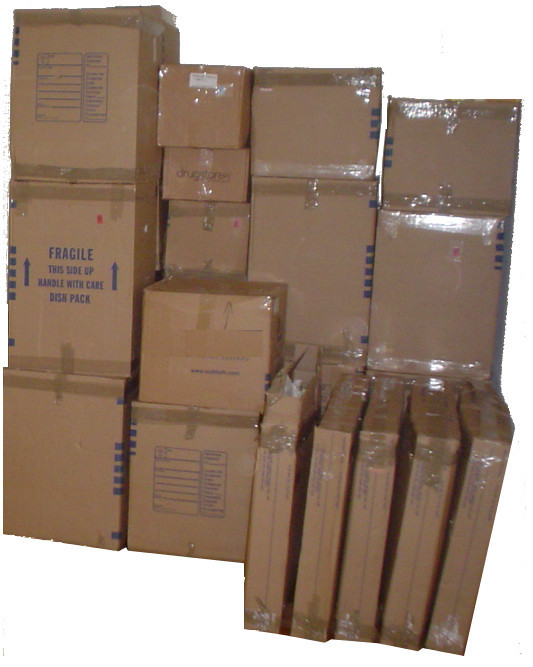
\includegraphics[width=.25\textwidth]{05/pics/many-boxes}
\end{figure}

\section{Introduction}
\label{software-installation:introduction}

%\begin{figure}[b]
%	\captionsetup{justification=justified,singlelinecheck=false}
%	\caption[Moving Boxes]{As anybody preparing a move knows,
%		handling all your boxes frequently ends in organized
%		chaos at best.  Managing software packages is not very	
%		different.
%		\label{fig:many-boxes}}
%\end{figure}


Having covered the details of file systems and storage
devices in the previous chapter, we can now focus on
installing an operating system and adding software
according to the intended purpose of the system.  Most
people never have to actually perform an OS
installation, but System Administrators are not most
people.  We routinely set up new systems, create new
services, and need to be able to fine-tune the
software from the very lowest layers, defining exactly
what software is installed, what drivers the kernel
needs to support, what modules it should load, and
what services should be started at boot time.

In addition, even within a single host, some subsystems
that control components on a lower layer than even the
OS kernel, such as a RAID controller or a Fibre
Channel \gls{hba}, are driven by their own
firmware\index{firmware}, accessed by the OS via its
kernel drivers and exposed to the administrative users
via additional software tools.  All of these types of
software have specific requirements, yet all of them
also have in common the general mechanisms to install,
update, maintain and remove the software.

In this chapter we will discuss in some detail the
general principles underlying all software
installations, beginning with a distinction of the
different types of software we commonly encounter,
most notably the two main categories of OS components
and {\em add-on} or {\em third-party} software.  We
will look at how an operating system is installed on a
server and what installation mechanisms are commonly
used.  Since different operating systems install
different components into different locations, we will
also take a close look at the file system layout and
explain some of the reasons behind the common
hierarchy found on most Unix systems.

Later in the chapter, we will cover concepts of
software package management that allow a system
administrator to not only add or remove software with
ease, but to help maintain software runtime
dependencies and provide a consistent way to upgrade
software when needed.  Unfortunately, software package
management is still not a solved problem: managing
software updates and security patches brings with it a
surprising number of complex problems, in part due to
competing solutions in this problem domain.  All of
this does not even touch upon the evolution of how
applications are bundled in the context of virtual
machines, virtual appliances, and software
containers\index{containers}. \\

Every system administrator has a preferred operating
system, and this preference is often the result of
years of experience and familiarity not only with the
kernel and libraries that make up the OS, but
frequently also due to the package management system
in use on the host.  Just how, exactly, a package
manager maintains software dependencies, what kinds of
assumptions it makes about the system it is running
on, its purpose, and its many uses all reflect deeply
on the OS development philosophy.  The way software
updates are handled speaks volumes about both the
system as well as its administrators -- the better we
understand software installation concepts, the better
we will be at managing our systems.  Understanding all
this just a little bit better is, in a nutshell, what
this chapter is all about.

\section{Types of Software}
\label{software-installation:types}
\index{Software!Types of}

In its most general definition, ``software'' is just
another term for a program telling a computer to
perform a certain task.  Practically, however, there
are a number of different types of software.  In this
section, we will attempt to categorize these types,
even though the distinctions or differentiating
factors are far from clear-cut.

In the previous chapter, we have already identified a
specific component that happens to be implemented in
software: the file system.  Instinctively, we
categorize the file system as being in a lower layer
than certain applications, such as a web server for
example.  But the file system is only one component of
the operating system, which in turn comprises regular
application software (such as a text editor or a
compiler), software libraries used by many of these
applications (such as the resolver library, used to
turn hostnames into IP addresses), device
drivers\index{device driver} providing access to and
control of certain hardware components, and the most
central component of the OS itself, the
kernel\index{kernel}.

Looking at software from this perspective quickly
makes it clear that the term ``operating system''
itself requires some definition, as different
providers include different components under this
umbrella term.  Recall from our discussion of the Unix
history in Section \ref{unix:history:os} that the term
``Linux'', for example, may refer to the linux
kernel as well as any number of ``distributions'',
each bundling a variety of components to make up a
version of the GNU/Linux operating system.  But before
we attempt to tackle the question of what, exactly,
defines an operating system, let us take a step back
and attempt to better categorize software based on its
proximity to the hardware or the end user.

\subsection{Up and down the software stack}
\label{software-installation:boot-sequence}

One of the most common systems a system administrator
may be in charge of is probably a generic
HTTP\index{HTTP} server, offering a web service of
some sort.  Such a service nowadays consists of a
perhaps surprising number of components and software
dependencies running -- in our example here, anyway --
on virtual hardware within the AWS cloud service.
From a "top down" perspective, it might:

\begin{itemize}
	\item require an HTTP server -- the actual d\ae mon
		handling the network connections on
		port 80 and 443
	\item require e.g. PHP, Perl, Python, Ruby, or Java --
		entirely static pages are seldom found
		on the internet; instead, most web
		servers provide dynamic content via
		integration with other programming
		languages and modules
	\item which use generic library functions --
		the web server and the programming
		languages or frameworks are utilizing
		the standard libraries available on
		the system
	\item which make various system calls (see
		our discussion in Chapter \ref{unix:basics})
	\item which the kernel handles for the OS
	\item which is running in a virtual machine\index{virtual machine} --
		in the case of AWS, the OS our server is
		running on does not actually sit on
		top of the hardware itself
	\item which is running on top of a {\em
		hypervisor}\index{hypervisor} -- the
		host system managing the hardware for
		the different {\em guest} OS, such as
		for example the Xen
		hypervisor\index{Xen}
	\item which uses firmware to manage various
		hardware components
	\item which, finally, is running on some
		hardware in a data center somewhere
\end{itemize}

Going down this stack, we can already identify a number of
different interacting and overlapping categories of
software.  As such a Unix system boots up, it goes
through a number of phases, each of which handled by a
different type of software.  The typical boot sequence
begins at a very low level close to the hardware and
with each step adds another layer of abstraction,
bringing the system closer to interaction with the
user.

In order not to complicate things more than absolutely
necessary, we will skip over the layers involving the
hypervisor in the following.  Pretending that the OS
runs on actual, not virtual hardware, the boot process
might then include these steps:

\begin{figure}[t]
	\subfloat[American Megatrends POST]{\label{fig:software-installation:post}
				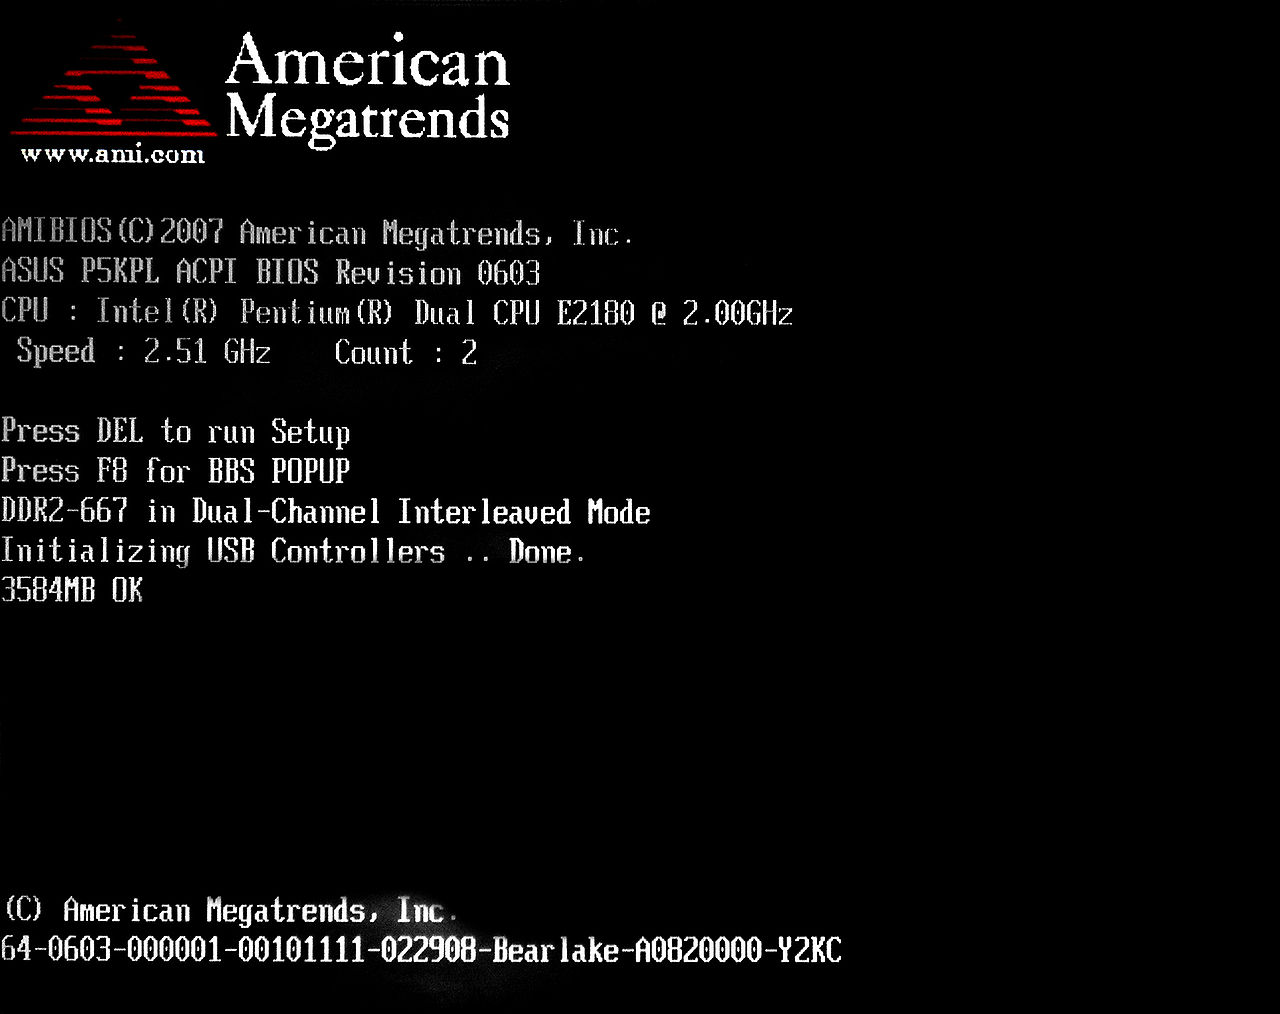
\includegraphics[width=.4\textwidth]{05/pics/POST}}
	\hspace{1em}
	\subfloat[Award Software BIOS]{\label{fig:software-installation:bios}
				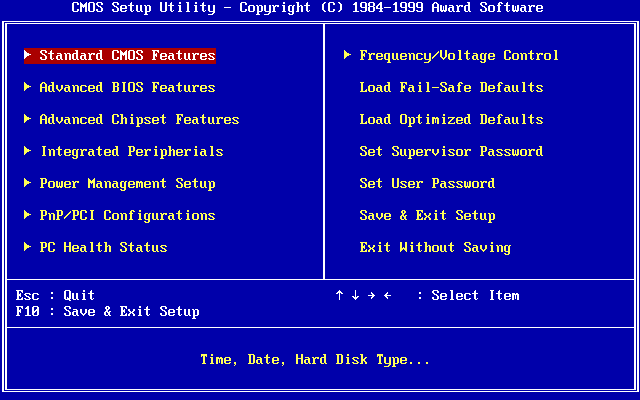
\includegraphics[width=.5\textwidth]{05/pics/BIOS}}
	\caption{A typical POST and BIOS screen}
\end{figure}

\begin{itemize}
	\item Power-On Self Test (\glslink{post}{POST}\index{POST}) -- a few very basic routines
		intended to insure the hardware is not obviously faulty;
		Figure \ref{fig:software-installation:post} shows a typical POST screen
	\item execution of the primary boot loader\index{boot loader!primary}
		-- a simple program stored in read-only memory; examples include
		the \gls{bios}\index{BIOS} (as shown in Figure
		\ref{fig:software-installation:bios}), \glslink{uefi}{UEFI}\index{UEFI},
		and OpenBoot\index{OpenBoot}/Open Firmware
	\item access of the \gls{mbr}\index{Master Boot Record} -- a special boot sector
		found on the primary boot device; the code found in this
		location allows the system to access the file system(s)
		and transfer control to a second-stage boot loader;
		see Chapter \ref{file systems:storage-models:dividing-and-combining-disks:partitions}
	\item execution of a secondary or second-stage boot loader --
		\index{boot loader!second-stage} a small program allowing
		the user to interactively choose an operating system or
		kernel to boot; examples include GRUB\index{GRUB} (Figure
		\ref{fig:software-installation:grub}) or
		{\tt boot(8)}\index{\tt boot(8)}
		(Figure  \ref{fig:software-installation:nbsdboot})
	\item loading of the hypervisor and starting
		of the privileged domain ({\em dom0}\index{Xen!dom0})
	\item initialization of the virtual hardware
		by the {\em domU} for the guest OS ({\em domU}\index{Xen!domU})
	\item loading of the guest OS kernel -- booting, initializing (virtual) hardware, loading
		modules
	\item \manpage{init(8)} -- one of the few processes created
		explicitly by the kernel, {\tt init(8)} spawns all other
		processes of the running OS and boostraps the final system
	\item starting of system services -- started by {\tt init(8)}, commonly via a
		number of shell scripts using e.g. the {\tt rc(8)}\index{\tt rc(8)} or
		{\tt /etc/init.d} frameworks
	\item the interactive system runs, presenting a login prompt; the web server
		accepts network connections and begins traffic
\end{itemize}

\newsavebox{\nbsdboot}
\begin{lrbox}{\nbsdboot}
\begin{minipage}{.7\textwidth}
\begin{lstlisting}[basicstyle=\scriptsize]
>> NetBSD/i386 BIOS Boot, Revision 5.2
>> (builds@b7, Sun Feb 7 00:30:50 UTC 2010)
>> Memory: 639/130048 k
Press return to boot now, any other key for boot menu
booting hd0a:netbsd - starting in 30
\end{lstlisting}
\end{minipage}
\end{lrbox}

\begin{figure}[t]
	\centering
	\subfloat[GNU GRUB]{\label{fig:software-installation:grub}
				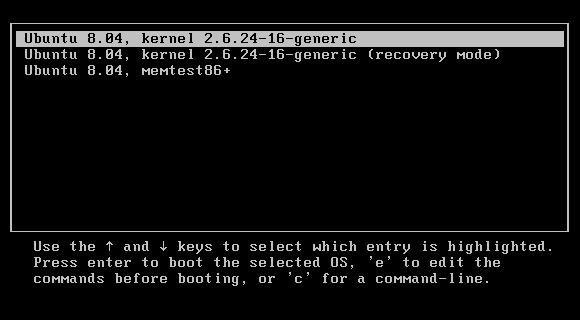
\includegraphics[width=.6\textwidth]{05/pics/grub}}
	\\
	\subfloat[NetBSD \manpage{boot(8)}]{\label{fig:software-installation:nbsdboot}
		\usebox{\nbsdboot}}
	\caption{Second stage boot loader examples}
\end{figure}

Most Unix systems display diagnostic messages from the
boot process on the system console\index{console} and
may retain a copy on the file system under e.g. {\tt
/var/run/dmesg.boot}.  The \manpage{dmesg(8)}
command can be used to display these messages.  On
Amazon's EC2 systems, you can use the {\tt aws ec2
get-console-output} command to retrieve the
information displayed on the (virtual) console.

Listing \ref{code:nbsdboot1} and \ref{code:nbsdboot2}
show the output on the serial console displayed during
the boot process of a NetBSD Amazon EC2
instance showing information from the hypervisor and
the virtualized guest OS respectively.

\begin{lstlisting}[float,basicstyle=\scriptsize,label=code:nbsdboot1,caption={Excerpt
of the boot messages of a NetBSD Xen
domU\index{Xen!domU} booting in
Amazon EC2}]
i-38d44816      Xen Minimal OS!
  start_info: 0xa01000(VA)
    nr_pages: 0x26700
  shared_inf: 0x7dcc4000(MA)
     pt_base: 0xa04000(VA)
nr_pt_frames: 0x9
    mfn_list: 0x967000(VA)
   mod_start: 0x0(VA)
     mod_len: 0
       flags: 0x0
    cmd_line: root=/dev/sda1 ro 4
  stack:      0x946780-0x966780
MM: Init
      _text: 0x0(VA)
     _etext: 0x61e65(VA)
   _erodata: 0x76000(VA)
     _edata: 0x7b6d4(VA)
stack start: 0x946780(VA)
       _end: 0x966d34(VA)
  start_pfn: a10
    max_pfn: 26700
Mapping memory range 0xc00000 - 0x26700000
setting 0x0-0x76000 readonly
skipped 0x1000
MM: Initialise page allocator for b3e000(b3e000)-0(26700000)
MM: done
Demand map pfns at 26701000-36701000.
Heap resides at 36702000-76702000.
Initialising timer interface
Initialising console ... done.
gnttab_table mapped at 0x26701000.
Initialising scheduler
Thread "Idle": pointer: 0x36702008, stack: 0xbf0000
Initialising xenbus
Thread "xenstore": pointer: 0x36702478, stack: 0x26600000
Dummy main: start_info=0x966880
Thread "main": pointer: 0x367028e8, stack: 0x26610000
"main" "root=/dev/sda1" "ro" "4" 
vbd 2049 is hd0
******************* BLKFRONT for device/vbd/2049 **********


backend at /local/domain/0/backend/vbd/1720/2049
Failed to read /local/domain/0/backend/vbd/1720/2049/feature-barrier.
Failed to read /local/domain/0/backend/vbd/1720/2049/feature-flush-cache.
2097152 sectors of 0 bytes
**************************
vbd 2050 is hd1
\end{lstlisting}

\begin{lstlisting}[float,basicstyle=\scriptsize,label=code:nbsdboot2,caption={Excerpt
of the boot messages of a NetBSD system}]
Copyright (c) 1996, 1997, 1998, 1999, 2000, 2001, 2002, 2003, 2004, 2005,
    2006, 2007, 2008, 2009, 2010, 2011, 2012
    The NetBSD Foundation, Inc.  All rights reserved.
Copyright (c) 1982, 1986, 1989, 1991, 1993
    The Regents of the University of California.  All rights reserved.

NetBSD 6.1.2 (XEN3PAE_DOMU)
total memory = 615 MB
avail memory = 597 MB
mainbus0 (root)
hypervisor0 at mainbus0: Xen version 3.4.3.amazon
vcpu0 at hypervisor0: Intel(R) Xeon(R) CPU E5-2650 0 @ 2.00GHz, id 0x206d7
xenbus0 at hypervisor0: Xen Virtual Bus Interface
xencons0 at hypervisor0: Xen Virtual Console Driver
npx0 at hypervisor0: using exception 16
xbd0 at xenbus0 id 2049: Xen Virtual Block Device Interface
xbd1 at xenbus0 id 2050: Xen Virtual Block Device Interface
xennet0 at xenbus0 id 0: Xen Virtual Network Interface
xennet0: MAC address 22:00:0a:47:89:0e
balloon0 at xenbus0 id 0: Xen Balloon driver
balloon0: current reservation: 629760 KiB
xennet0: using RX copy mode
balloon0: current reservation: 157440 pages => target: 157440 pages
boot device: xbd1
root on xbd1a dumps on xbd1b
root file system type: ffs
Sat Feb  1 21:46:17 UTC 2014
Starting root file system check:
/dev/rxbd1a: file system is clean; not checking
Starting file system checks:
/dev/rxbd0a: file system is clean; not checking
Setting tty flags.
Setting sysctl variables: ddb.onpanic: 1 -> 0
Starting network.
IPv6 mode: host
Adding interface aliases:.
Building databases: dev, utmp, utmpx, services.
Starting syslogd.
Mounting all filesystems...
Clearing temporary files.
Generating public/private rsa1 key pair.
Your identification has been saved in /etc/ssh/ssh_host_key.
Your public key has been saved in /etc/ssh/ssh_host_key.pub.
The key fingerprint is: ca:b3:e5:45:20:69:94:bf:ef:92:69:da:32:7b:1e:cc
Starting sshd.
Starting local daemons:.
Updating motd.
Starting powerd.
Starting inetd.
Starting cron.
Sat Feb  1 21:46:37 UTC 2014

NetBSD/i386 (ip-10-71-137-14.ec2.internal) (console)

login:
\end{lstlisting}

At each step of the boot process, we find a different
type of software active as the dominant component.  At
the final stage, when the system is up and running, we
can easily identify certain applications or services
that interact directly with the user.  This kind of
software does not require any special privileges and
does not rely on any particular hardware.  Even
though these applications may have a dependency on
specific features or capabilities in the OS, they are
effectively isolated from the kernel's privileged
execution mode.  They are entirely optional and
installed by the system administrator as needed;
common examples include a web browser or a database
management system.  In this book, we use the term
``add-on'' or ``third-party''
software\index{Software!Add-on}\index{Software!Third-Party}
to indicate that it was not included in or
distributed directly with the operating system.

Below these software packages exists a layer of
software applications and system utilities without
which the OS would simply not be complete.  All of the
common Unix utilities\index{Software!System Utilities}
such as \manpage{awk(1)} \manpage{sed(1)}, or even
\manpage{ls(1)} fall into this category, as do the
common system d\ae mons such as \manpage{sshd(8)} or
\manpage{syslogd(8)}, to name but a few.  The standard
Unix command interpreter, the shell, is part of this
layer, and most systems include a compiler chain and
other basic development tools as well.  Like add-on
software packages, this software also relies on a
number of basic OS capabilities, which form another
(sub-)category: the system libraries, kernel modules,
and device drivers used by applications to interact
with the OS kernel, the next layer in our software
stack.

We can define the kernel as the central component of
the operating system in charge of process-, device-
and memory management, facilitiating access to the
hardware via a small number of {\em system
calls}\index{system calls}.  Software running in the
kernel's address space has full access to all aspects
of the hardware and OS, while software running in
so-called ``user space'' relies on the kernel or the
system libraries to provide access to these resources
when needed.

Finally, we have a layer of software that falls
somewhat in between the kernel and the system
software: some of the physical resources maintained by
the kernel rely on hardware controllers providing
increasingly complex code running in persistent memory
on the devices themselves.  Since this software,
frequently consisting of low-level microcode, exists
somewhat in between the clearly defined categories of
{\em hardware} and {\em software}, it is commonly
referred to as {\em firmware}\index{firmware}.
Besides the previously mentioned RAID controllers or
Fibre Channel \gls{hba}, the most common example of
firmware here is probably the \gls{bios}.

Even though firmware can be viewed as residing
``below'' the kernel, closer to the hardware, many
systems provide tools to interact with or update the
firmware from within the OS.  Some of this software
requires the kernel to facilitate this access, for
example via a loadable module.  Likewise, the
previously mentioned bootloader is an independent
program executing outside the OS kernel, but from
within the OS we can manipulate its behaviour and
configure it to change the way the system is booted.

It is also worth mentioning that some code is executed
exactly once (POST, the bootloader), while other
low-level components (kernel modules or RAID firmware,
for example) are used periodically or continually
throughout a system's running time.  Once again, the
distinction between what constitutes optional add-on
software, an essential system component, or low-level
access to the hardware by the kernel is far from
obvious.

\subsection{Operating System vs. System Software vs. Third Party Software}
\label{software-installation:system-vs-third-party}
\index{Software!Distinction between different types of}

Our attempt to draw the software stack as described in
the previous section is illustrated in Figure
\ref{fig:software:types}.  As we review these layers,
it quickly becomes obvious that unfortunately the
distinctions are not as well-defined as we would like
them to be.

It has become increasingly difficult to clearly
identify any given piece of software as being an
``add-on package'', as OS providers include more and
more software in their distributions in order to make
their product suitable for the widest variety of uses.
Many Linux distributions, for example, include the
canonical examples cited above (web browsers, database
management systems, web servers, etc.), as they target
both the server and desktop markets, while the BSD
derived systems tend to favor a leaner setup,
explicitly targeting the server market.

But what exactly defines an operating system?  It is
clear that an OS cannot exist without a kernel, but on
the other hand a kernel all by itself does not provide
for a useful environment, either.  For this reason,
different providers bundle the kernel with {\em system
software} (device drivers, loadable kernel modules,
core libraries etc.) and {\em system utilities} (such
as a shell, the various command-line utilities, system
d\ae mons, development tools etc.).  The more closely
coupled these components are, the more coherent the
resulting OS is.  Many core system libraries rely on
the presence of certain features in the kernel, and
not keeping these components in sync or even replacing
one or the other tends to introduce a significant risk
of instability.

For this reason, many OS providers only support their
own specific releases of the many system components in
their specific software bundle.  If you replace parts
of the system (either the kernel, core libraries, or
various important system components), you are breaking
up the bundle of software that initially made up the
given release of the OS in question.  You are in
effect creating a different version, a different
``distribution'' of the OS.\footnote{ Nowadays, the
term is more commonly used when referring to a
specific Linux flavor, but recall from Chapter
\ref{unix:history:os} that the ``D'' in ``BSD'' stands
for ``distribution'': the idea of bundling different
software packages and making them available as a
well-defined release has been around for quite some
time.}

Many Unix versions come in only exactly one flavor,
one bundle of kernel plus libraries plus system
utilities -- the open source BSD versions and
virtually all of the ``old'' commercial Unix versions
fall into this category.  Releases differ across time
in features added or removed, but a given version of
the OS will behave the same way anywhere you may
encounter it.

Contrast this with the world of Linux, where the
definition of a coherent operating system has been
replaced with variety in software bundling: a common
kernel (possibly with custom modifications) combined
with the core libraries from the \gls{gnu} project and
a suprising variety of different add-on software.
Some of these ``distributions'' replace core system
utilities, some remove components but add others etc.,
until they behave sufficiently different from one
another that they may well be regarded as unique Unix
flavors.  \\

\begin{figure}[t]
	\centering
	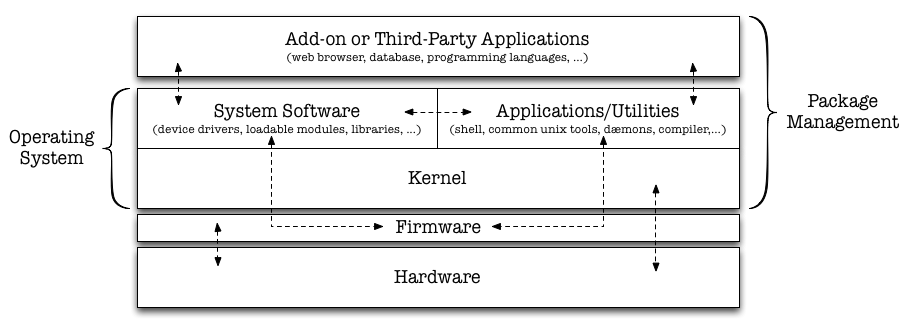
\includegraphics[width=.85\textwidth]{05/pics/types-of-software}
		\caption[Types of Software]{We define a software layer
			stack consisting of ``Add-on Applications'',
			``System Software'' and
			``Applications/Utilities'', the kernel, and
			firmware, some of which may be controlled via a
			package management system.  Interactions between
			these types are illustrated as arrows, but it is
			important to note that none of these distinctions
			are precise.
			\label{fig:software:types}}
\end{figure}


As different OS providers disagree on what components
should be part of their final product, it becomes very
difficult to declare a software package to belong into
any one of the categories we've defined.  However,
most system administrators ultimately develop an
instinctive idea of what should or should not be
considered {\em essential}, what can and cannot be
removed from the system without unexpected side
effects, and which components may only be upgraded in
sync with kernel- or system library upgrades.

This understanding comes with years of experience, and
it helps to think about software in terms of their
place in the software stack we have defined.  As so
often, we end up creating flexible definitions that
allow us to translate core concepts across variable
implementations.  We will see throughout this chapter
how this approach will help us understand the
installation- and upgrade process, the placement of
software within the file system hierarchy, how system
configuration files and software runtime changes are
handled and hopefully gain a better understanding of
how to tune and maintain our systems.

\section{File System Layout}
\label{software-installation:file-system-layout}

In Section \ref{file systems:layout}, we briefly
summarized the hierarchical tree-like structure of the
Unix file system layout and noted that the purpose or
common use of the different subdirectories as
described on many Unix versions in the {\tt hier(7)}
manual page.  Unfortunately, this layout is not
standardized and different versions of Unix have, for
historical reasons as well as purely by coincidence or
developers' preferences, diverged.  But almost all
Unix versions do still share a number of common
directories, especially as far as the base OS is
concerned.

In the early days of Unix, disk space was still
expensive, and it was not uncommon to split the files
of the operating system across multiple devices.  As
the system boots up, it obviously requires a number of
files to be present and services to run before it can
mount any other partitions or disks.  For this reason,
Unix systems used to have a small root partition
(mounted at {\tt /}, pronounced ``slash''), sufficient
to boot the OS, with additional software stored on a
separate disk, commonly mounted under {\tt /usr}.
{\tt /} contained all the system binaries (found in
{\tt /bin}) and libraries (found in {\tt /lib}) to
perform basic system maintenance, while so-called
``user'' binaries and libraries were found in {\tt
/usr/bin} and {\tt /usr/lib} respectively; the use of
the different {\tt bin} and {\tt lib} directories
themselves already hints at a clear definition of
purpose.

Since costs for disk space have come down so far as to
no longer be a limiting factor, it is nowadays rare to
find a Unix system that actually has {\tt /usr} on a
separate device from the root partition.
Nevertheless, this historical distinction remains
useful: it illustrates careful forethought with
regards to the placement of and interactions amongst
software components, which is worth reviewing in
detail.  Listing \ref{code:hier} shows an excerpt of
the \manpage{hier(7)} manual page on a NetBSD system.  The
definitions there overlap with those given in the
``Filesystem Hierarchy Standard''\index{Filesystem
Hierarchy Standard}\cite{fhs}, a formalization of this
same old hierarchy overseen by the Linux
Foundation\index{Linux Foundation}.

\begin{lstlisting}[float,basicstyle=\scriptsize,label=code:hier,caption={Excerpt of the {\tt hier(7)} manual page.}]
NAME
    hier -- layout of filesystems

DESCRIPTION
    An outline of the filesystem hierarchy.

    /          root directory of the system

    /bin/      utilities used in both single and multi-user environ-
               ments

    /etc/      system configuration files and scripts

    /lib/      dynamic linked libraries used by dynamic linked programs
               (such as those in /bin/ and /sbin/) that cannot rely
               upon /usr/lib/ being available.

    /libexec/  system utilities (such as the dynamic linker) required
               by programs and libraries that cannot rely upon
               /usr/libexec/ being available.

    /sbin/     system programs and administration utilities used in
               both single-user and multi-user environments


    /tmp/      temporary files, usually a mfs(8) memory-based file
               system (the contents of /tmp are usually not preserved
               across a system reboot)

    /usr/      contains the majority of the system utilities and files

               bin/      common utilities, programming tools, and
                         applications

               lib/      archive, profiled, position independent
                         archive, and shared libraries

               libexec/  system daemons & system utilities (executed
                         by other programs)

               sbin/     system daemons and system utilities
                         (normally executed by the super-user)

               share/    architecture-independent text files

    /var/      multi-purpose log, temporary, transient, and spool files

               log/      miscellaneous system log files

               run/      system information files, rebuilt after each
                         reboot

               tmp/      temporary files that are not discarded
                         between system reboots

SEE ALSO
     apropos(1), ls(1), whatis(1), whereis(1), which(1), paths(3)

HISTORY
     A hier manual page appeared in Version 7 AT&T UNIX.
\end{lstlisting}

Due to the previously mentioned traditional separation
of {\tt /} and {\tt /usr}, it is not surprising to see
a similar subtree reflecting the root file system
under {\tt /usr}.  That is, we find subdirectories
named {\tt bin}, {\tt lib}, {\tt libexec}, {\tt sbin}
and {\tt share}, with each having a similar purpose as
under the root.  On many systems, we also find the
{\tt /usr/local} directory as a specific location for
files that are not part of the base OS.  This
directory has become the default location for any
``add-on'' software, and it is thus not very
surprising that it also mirrors the general root
hierarchy to some extent.

Note that {\tt /usr} contains a subdirectory named
{\tt share} for so-called ``architecture independent
data-files''.  As the name suggests, the files in this
location are intended to be able to be shared across
multiple system.  Another directory with a
particularly descriptive name is {\tt /var}, for
``variable'' or transient data, known to change at
runtime.

These two directories already hint at two major
properties of files found on any Unix system, each
with distinct implications on where or how they might
best be organized\cite{fhs}, and each deriving from
standards and best practices of the early days of
Unix: \\

{\bf Shareable} versus {\bf unshareable} content:
Data files that remain the same across multiple hosts,
and, as the manual page suggests, possibly even across
different hardware architectures are considered {\em
shareable}.  Flat text files or simple system
databases that are not used for runtime configuration
such as manual pages, timezone or terminal
information, are good examples.\footnote{It should be
noted that across hosts of a uniform hardware
architecture most binaries are also common candidates
for shareable directories, and it was, in fact, not
uncommon for multiple hosts to share {\tt /usr}, for
example.  Nowadays, such a setup is a rare exception.}
This data frequently remains unchanged throughout
day-to-day operations -- that is, it only changes if
it is intentionally and specifically updated.  Note
that these files may at times overlap with some
``local'' data (i.e. files not included in the base
OS).

Data files that need to be individual to each host are
considered {\em unshareable}.  Sometimes this is due
to the fact that the data simply changes at runtime
(such as a sytem's log files), other times it is
because these files define a unique feature of a given
host (most files under the {\tt /etc} directory fall
into this category).  Note that once again these files
may at times overlap with certain ``local'' data.  \\

{\bf Static} versus {\bf variable} data:  Files that
are not expected to change during the runtime of the
system are considered {\em static}.  This includes the
kernel, all system libraries and binaries and many
data files.  Note that these files may, of course, be
changed when the system is upgraded, for example, but
are not modified under normal circumstances.

Files that are updated by the OS, by any running
applications or by end-users at runtime, are termed
{\em variable}.  That is, we anticipate that these
files will be created, modified, updated, or removed.
Some may see frequent or even continous updates (such
as the various log files), while others only see
comparatively rare modifications (such as when a
system d\ae mon is restarted).  \\

Combining these four classes of data yields a matrix
of files with common locations in the file system
hierarchy as illustrated in Table
\ref{table:software-installation:shareable-variable}.
Note that not all static data is necessarily
shareable, just as not all variable data is
necessarily unshareable.

\begin{table}[b]
\centering
	\begin{tabular}{ l l l }
	& shareable content & unshareable content \\
	\hline
	static data & {\tt /usr} & {\tt /boot} \\
	& {\tt /opt} & {\tt /etc} \\
	\hline
	variable data & {\tt /var/mail} & {\tt /var/run} \\
	& {\tt /var/spool/news} & {\tt /var/lock} \\
	\hline
	\end{tabular}
	\caption[Shareable/unshareable vs. static/variable files]{Typical
		examples of shareable/unshareable vs. static/variable files.}
	\label{table:software-installation:shareable-variable}
\end{table}

Even though nowadays it is less and less common for
multiple Unix system to share specific directories or
mount points (perhaps with the exception of users'
home directories, which are still frequently accessed
over a network file system), the distinction of
variable versus static data is of particular
importance.  Carefully separating these kinds of data
will allow you to build systems with separate mount
options for these types, which can improve performance
and security significantly.  As examples, consider a
read-only partition for system binaries to prevent
accidental or malicious writes to the base OS, or
mounting a directory containing system logs using the
{\tt noatime} or {\tt noexec} mount
options.\footnote{Reference your \manpage{mount(8)} manual
page for details.  Many other options are available.}

Understanding these criteria also helps make sense of
why software providers choose a certain location for
their files, or how different package managers may
apply the file system hierarchy standard.  Beware,
however, that not all software providers necessarily
understand or follow this matrix or even the general
Unix conventions!

\section{OS Installation}
\label{software-installation:os-installation}

System administrators often maintain large numbers of
hosts, and so it comes as no surprise that new
machines -- both physical and virtual -- have to be
brought up and integrated into the infrastructure on a
regular basis.  The more systems are maintained and
created, the more this process needs to be automated,
but at the end of the day, each one follows the same
set of common steps.  In an ideal world, these steps
could be summarized as requiring the installation of a
base operating system with subsequent adjustments for
the specific task at hand.

As we will see in this section, each step depends on a
large number of variables and site-specific
customizations, and so most large-scale organizations
have written their own automation framework around a
few common tools to accomplish the goal of quick and
scalable system and service deployment.  In fact, the
topic of automated deployment tools is too large to
adaequately cover here (though we will revisit it in
later chapters) and we shall instead focus on the
essential concepts needed to understand the
requirements for such systems.

Installing a new system is a process unique to each
OS; installation methods range from unattended
deployment systems using information determined at
runtime to create the correct configuration to
interactive graphical installers (such as seen in
Figure \ref{fig:os-installation:opensolaris}) allowing
users to select amongst common options to create a
general purpose Unix server.  Understanding the
individual steps included is valuable, and we
recommend strongly for students to perform this task
as a learning exercise (see Problems
\ref{prob:software-installation:os-installation} and
\ref{prob:software-installation:os-installation:manual}):
sooner or later, any system administrator will find
him or herself trying to debug a broken installation,
and understanding all the steps performed and what
things might have gone wrong in the process are
invaluable.

\begin{figure}[t]
	\centering
	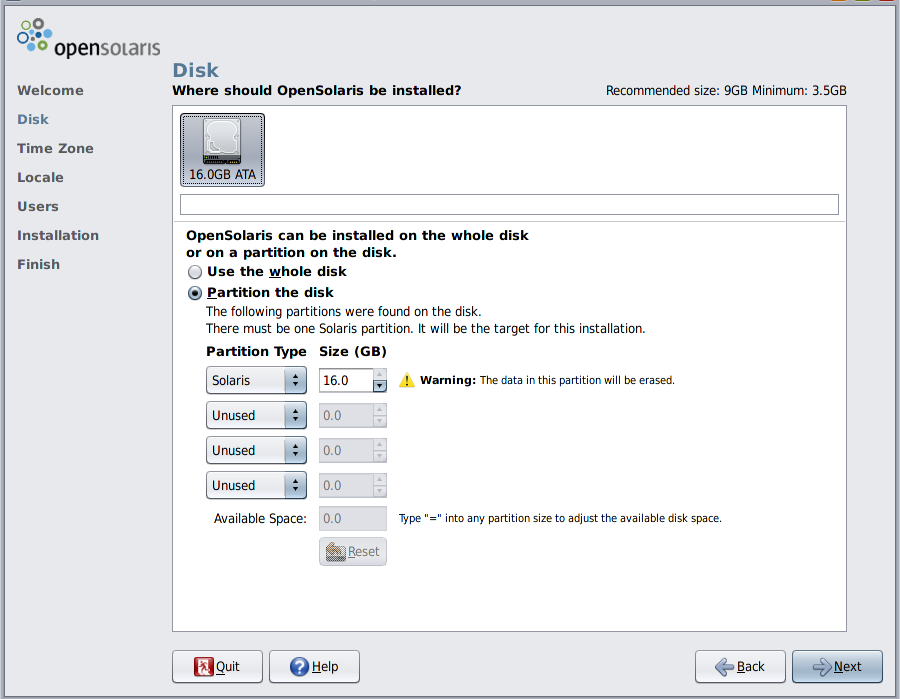
\includegraphics[width=.85\textwidth]{05/pics/opensolaris-install}
		\caption[OpenSolaris Installation]{A graphical installer
			showing an interactive disk partitioning tool.
			\label{fig:os-installation:opensolaris}}
\end{figure}

\subsection{Identifying server requirements}
\label{software-installation:os-installation:requirements}

Before a system is installed, a number of important
choices have to be made: What file system will be
used?  What are the requirements of the final system
with respect to file I/O?  How many partitions will be
created?  What OS will be installed?  What add-on
software?  What is the final purpose of the machine?

Many of these questions are interdependent and
answering one may restrict possible answers to other
questions.  For example, if the purpose of the server
is to run a specific piece of software that is only
available for a given OS, then this might also
influence a very specific partitioning schema or other
file system considerations.  In fact, the final
purpose of the machine and the software it needs to
run will likely dictate your hardware choices --
processor architecture, amount of memory and disk
space, number or types of network interfaces -- which
in turn restrict your OS choices.

For example, if you plan on building a highly
performant database server able to handle a large
number of transactions per second, you can quickly
identify the number of CPUs and CPU speed needed, the
size of RAM to provide a large in-memory buffer cache,
as well as hard drive disk speed and network
throughput requirements, but not all operating systems
are able to handle with equal efficiency the same
amount of CPUs, RAM, or perhaps link
aggregation\index{link aggregation}, for example.  As
a result, your database server may {\em have to} run
e.g. Solaris, even though the rest of your hosts are
all running Linux (or vice versa).

On the other hand, it is possible that the cost of
running a different OS just for one purpose is not
worth the benefit of running the theoretically ideal
software.  Instead, you might prefer to change your
infrastructure architecture and perhaps scale the
database horizontally across a number of smaller
commodity hardware systems to meet the requirements.
Whichever approach you choose, these design decisions
need to obviously be made prior to the OS installation
itself -- changing your OS later on often results in
much higher costs, as services have to be migrated,
ported, and verified while the server is already in
production use, a process that has been likened to
changing one's tires on a car travelling on a busy
highway at 100 miles per hour.

\subsection{OS Installation Overview}
\label{software-installation:os-installation:overview}

On a high level, the OS installation process itself consists of a few
distinct phases:

\begin{itemize}
	\item {\bf Hardware identification, provisioning and registration.}
		Before a new system can be installed, suitable hardware
		needs to be identified, physically installed, and
		registered with the inventory system.  Depending on the
		size of your organization, this may be a manual step
		performed immediately before the OS installation is
		started, or it might be done continously in a data center
		where hardware is racked, asset tags scanned and
		information automatically entered into a pool of
		``ready to install'' systems.

	\item {\bf Base OS installation.}
		The installation of the software itself.  Even though
		any reasonable deployment system combines these steps,
		we distinguish between the basic OS and additional
		software added (or unused components removed), to more
		clearly illustrate at which point in the process
		customization to our needs tends to happen.

	\item {\bf Installation of add-on applications.}
		In this step, we transform the generic OS into a server
		with a specific purpose.  The installation of the right
		add-on applications may entail fetching software updates
		over the network from a remote system or even building
		binaries from sources on the fly.

	\item {\bf Initial minimum system configuration.}
		After all software has been installed, a number of very
		basic configuration steps have to be performed.  This
		phase may include setting a hostname, applying a specific
		network configuration, adding user accounts or enabling
		certain system d\ae mons.  Note that in most cases a {\em
		configuration management system}\index{Configuration Management} is installed, which
		will perform this (and then ongoing) customization.

	\item {\bf System registration.}
		When all software is installed and configured and the system
		is ready to run and fulfill its purpose, we need to integrate
		it into our larger infrastructure.  Our inventory of which
		systems perform which function needs to be updated, our
		monitoring system needs to be made aware of this host, other
		components with which this server interacts may need to be
		updated etc.  It is important to consider this
		``paperwork'' to be part of {\em installation}, lest it be
		deprioritized or forgotten.

	\item {\bf System restart.}
		Finally, the system needs to be rebooted at least once
		before it is put into service.  This ensures that it can
		boot off the right media, all d\ae mons start up, the
		network is functional, the system can be monitored and in
		general everything behaves exactly as it should.  It is
		important to always include this step: during the
		installation process the system is in a very different
		state than under normal circumstances, and it is possible
		to forget to enable or disable a service.  Placing the
		system into production use without a fresh reboot might
		lead to unexpected results when the system is rebooted at
		a later point.
\end{itemize}

Obviously, each of these steps consists of many
smaller substeps; how exactly each of these main
objectives is accomplished depends heavily on the size
of the organization, the resources available, and the
level of automation required.  In addition, there is a
thin line between {\em system deployment}\index{system
deployment} and {\em system configuration}.  As
mentioned, the OS installation always includes at the
very least a few minimal configuration steps, but some
of the steps noted above may be considered part of a
configuration management system's first run.  That is,
much like the distinction between add-on software and
core system components, there exists a discrepancy
between what aspects of a server's configuration are
to be defined at installation time and which ones are
dynamically determined at runtime.  We will cover this
in more detail in Chapter
\ref{chap:configuration-management}; for the time
being, let us merely state that one way or another the
system, once completely installed and set up, is
configured for its final purpose.

\begin{experience}
{\bf Magic Deployment} \\

Around early 2007, during my time at Yahoo! Inc., I
worked together with a number of people on a
deployment system suitable to quickly build new Unix
systems and bring them up, ready to serve production
traffic.  As so many other shops, we, too, chose to
develop our own solution instead of using an existing
commercial or open-source system for this purpose.
Our setup was ``special'', unique, different from
whatever the existing solutions provided -- just like
everybody else's. (For what it's worth, this also
well predates scalable deployment engines and other
\gls{iaas}\index{Infrastructure!As a Service}
solutions such as e.g. OpenStack\index{OpenStack}.) \\
[10pt]

As a friend of mine once remarked,
you're not truly a system administrator until you have
written your own deployment system. Or configuration
management system.  Or inventory database.  Or
parallel secure shell to perform tasks across all of
your host.  Or... \\ [10pt]

Anyway, the system we wrote was elegant, and it taught
us a lot about the details of the OS installation
process.  Our goal was to allow hardware to be
delivered to the datacenter, be physically racked and
their asset tags scanned, and then not require any
more physical contact to be deployed, while at the
same time allow existing systems to be rebuilt or
decommissioned as needed. \\ [10pt]

Our final solution used IPMI\index{IPMI} to power on
the host, DHCP\index{DHCP} to assign a system {\em
profile} to the hardware (derived from a central
database, where the system was identified by the asset
tag), and a {\tt pxeboot}\index{pxeboot} process to
run the system through a number of stages.  In the
initial stage, the system would power up, identify and
apply any pending firmware upgrades, and then check if
it was ready to be deployed.  If not, it would go into
a special ``inventory'' state and power down. \\
[10pt]

When a number of hosts (frequently in the order of
tens or hundreds) had to be deployed, the system would
select suitable hardware from the pool of
``inventory'' systems, power them on, send them
through the initial stage again -- since it was
possible that a lot of time had passed since they were
first provisioned, additional firmware updates might
have been necessary -- and then enter the OS-specific
installation phase. \\ [10pt]

In this phase, the server was configured for its final
purpose: the correct OS and network configuration was
installed, software packages were deployed according
to the systems' profiles, user accounts added and
finally the system registered in the central database
as being ready for production traffic. \\ [10pt]

We programmed this system from afar, but the first
time we went to a datacenter to see it in action, we
were pleasantly surprised how well it worked: without
any physical interaction, we could see racks of
servers suddenly power up, install, reboot and start
taking traffic based on a simple hardware provisioning
request. \\ [10pt]

Arthur C. Clarke\index[names]{Clarke, Arthur C.} once remarked
that ``any sufficiently advanced technology is
indistinguishable from magic'', and so we proudly
named the project ``Magic Deployment''.  Three years
later, the system was obsoleted by a new, more
flexible system, re-written from scratch, ready to
adapt to the evolving requirements of this large
company...
\end{experience}

\subsection{OS Installation Details}
\label{software-installation:os-installation:details}

The list of phases outlined in the previous section
can be further refined.  It is clear that a number of
these steps are likely (and necessarily) dependent on
and intricately intertwined with a number of your
organization's infrastructure components, such as an
inventory system or a database keeping track of
configuration types or service roles, for example.

This integration into the larger infrastructure
ecosystem of a company tends to be complicated, which
is why most of these organizations end up writing
their own custom software for this purpose.  However,
eventually all of these systems, be they custom,
proprietary, public, open source, developed by the OS
provider or by a third party -- all of them have to
perform the same basic steps to actually get the OS
onto the disks.  Most installers hide the details of
these steps from the ordinary end-user, but, hey,
we're system administrators -- let's take a look under
the hood!  \\

\begin{enumerate}

	\item {\bf Boot the system.}\footnote{Note:
		with an eye towards security, we
		should mention in this context the
		concepts of {\em trustworthy
		computing}\index{trustworthy computing} and
		e.g. {\em hardware attestation}\index{hardware attestation},
		which may provide assurance that the
		system has not been tampered with
		prior to our booting it.  We will
		revisit this important topic in some
		detail in Chapter
		\ref{chap:security}.}
		This entails a decision of which
		media to boot from.  Manual installations tend to be
		performed by booting from a CD/DVD, while automated,
		unattended installs have for years relied on booting
		the system from the network using the {\em \gls{pxe}},
		\index{PXE}\index{pxeboot}
		which utilizes a combination of protocols such as {\em
		DHCP}, {\em TFTP}, {\em NFS} and/or memory-based
		filesystems to load a small version of the OS -- such as,
		for example, the Linux {\em initial ramdisk} ({\tt initrd(4)}) --
		which then performs all the steps to actually install the final
		system.

	\item {\bf Identify disk(s).}  Once booted, the install
		process needs to identify all available disks.
		This requires the ``miniroot'' to include or be able to load
		any drivers required to access the storage devices in
		question.

	\item {\bf Create partition table(s).}  Before the system can be
		installed, the disks identified in the previous step need
		to be partitioned.  This includes both the creation of a
		suitable \gls{bios} partition table (via e.g. \manpage{fdisk(8)}
		and/or the OS-specific disk label such
		as \manpage{disklabel(8)}).  At this step, we also need to
		decide on which of the available disks will become the
		target root device, i.e. which will contain the root
		file system, and where the other disks and partitions will
		be mounted later on.

	\item {\bf Create file system(s).}  Each partition defined in the
		previous step needs to be formatted for its respective
		file system.  It is important to pass the correct flags to
		\manpage{mkfs(8)}/\manpage{newfs(8)} since, as we
		discussed in Section \ref{sec:unix-file-system}, most file
		system features cannot (easily) be tuned at run time.

	\item {\bf Make the system bootable.}  At some point after the disks
		have been partitioned and before the host is rebooted for
		the first time, it needs to be made bootable.\footnote{The order
		of this step is not important, but leaving it out
		will yield a server unable to start up without
		manual intervention.}  The details depend again on the OS
		in question, but generally involve the installation of the
		disk bootstrap software in the \glslink{mbr}{MBR}\index{Master
		Boot Record} and the configuration of the first and second
		stage boot loader, for example via \manpage{installboot(8)} or
		\manpage{grub(1)}.

	\item {\bf Install the OS.}  Finally we have reached the point
		where the actual OS is installed.  This generally requires
		the retrieval of the system's base packages or archive
		files from a CD or DVD, via \gls{nfs} from another server or
		(perhaps via FTP) from a remote host (an approach which
		brings with it a number of security implications --
		how do you verify source authenticity and integrity? --
		and in which case initial network configuration of the
		miniroot system is a pre-requisite).

		After the data files have been retrieved, they are
		extracted or the necessary packages installed into the
		target root device.  Many interactive installers allow the
		user to select different sets of software to install
		and/or will automatically identify additional packages as
		required.

	\item {\bf Install add-on software.} After the base OS has been
		installed, any optional software may be added, based on
		either the system's configuration or interactive user
		input.  Depending on the installer, this step may be
		combined with the previous step.  We explicitly note this
		as a separate step, since ``add-on'' software here may not
		only include optional packages from our OS vendor, but
		also your own software, such as your configuration
		management system, third-party applications licensed to
		your organization, or your software product or serving
		stack.

	\item {\bf Basic system configuration.}  As we mentioned before,
		any server requires ongoing maintenance that, in large
		part, is performed by automated systems performing
		configuration management.  But regardless of whether or
		not such a (complex) system is integrated into the OS
		installation process, there are a few things that need to
		be defined at install time.  This usually includes
		a host's network configuration and hostname, timezone, NTP
		and syslog servers, root password, and services started at
		boot time, to name just a few examples.

	\item {\bf Reboot.}  Finally, after the system has been installed
		and basic configuration performed, it needs to be
		rebooted.  At this time, the host boots the way it would
		under normal circumstances and enters a ``first boot''.
		This stage in a host's deployment process tends to be
		significantly different from a normal boot:  a number of
		services are run for the first time, and further initial
		system configuration and system registration (as noted
		above) is likely to take place.

		Since this initial boot sequence may install software
		upgrades and change the runtime configuration, it is
		advisable to reboot the host {\em another} time
		after this ``first boot''.  This ensures that the system
		does in fact come up in precisely the same state as it
		would in the future.

\end{enumerate}

Listing \ref{code:netbsd-install} shows the most basic
steps to perform a minimal OS installation.  It is
interesting to analyze each of them (and constrast the
sequence for different operating systems), as doing so
often illustrates a number of assumptions made about
the use of the software.  The ease with which an OS
installation can be automated (at scale!) shows how
much the OS provider has prepared their system for a
wide variety of use cases.  System defaults, such as
what services are enabled and started by default,
speak volumes about general design philosophies.
Similarly, the selection of software bundled with the
OS reflects on the target audience for a given OS.

Deploying a new host requires more than just
installing an operating system, however.  The system
needs to be incorporated into our larger
infrastructure, which may entail updates to a number
of inventories or databases that keep track of an
organizations assets or the various hosts' purposes.
This integration is necessarily very different from
site to site and unfortunately frequently not suitably
abstracted into a general \gls{api} that an installer
might integrate with.  As a result, most system
administrators do end up writing their own deployment
system and/or helper tools, calling into the various
operating systems' specific installers, and adding
their own customizations.

One of the many customizations included in any
software deployment system includes the extent to
which add-on software is controlled.  Getting the
right software onto the machine is part of the
installation process, but there is more to managing
applications and configuration files than copying
files from one place to another.  In the next section,
we will take a closer look at this topic.

\begin{lstlisting}[float,basicstyle=\scriptsize,label=code:netbsd-install,caption={[Commands
used during the installation of NetBSD]Manual
installation of NetBSD using the \manpage{fdisk(8)},
\manpage{disklabel(8)}, \manpage{newfs(8)}, and
\manpage{installboot(8)} commands.}]
# fdisk -f -u -0 -s 169/63/4194241 /dev/rwd0d
# fdisk -f -c /usr/mdec/mbr /dev/rwd0d
# fdisk -f -a -0 /dev/rwd0d
# disklabel -e -I wd0
[...]
4 partitions:
#      size   offset fstype [fsize bsize cpg/sgs]
a:  4194241       63 4.2BSD    0     0      0 # (Cyl.      0*- 4161*)
c:  4194241       63 4.2BSD    0     0      0 # (Cyl.      0*- 4161*)
d:  4194304        0 unused    0     0      0 # (Cyl.      0 - 4161*)
# /sbin/newfs -O 2 /dev/rwd0a
/dev/rwd0a: 2048.0MB (4194240 sectors) block size 16384,
        fragment size 2048 using 12 cylinder groups of
        170.67MB, 10923 blks, 21504 inodes.
super-block backups (for fsck_ffs -b #) at:
32, 349568, 699104, 1048640, 1398176, 1747712, 2097248, 2446784,
....................................................................
# mount -o async /dev/wd0a /mnt
# for pkg in base comp etc games man misc modules text kern-GENERIC; do
        tar zxpf /i386/binary/sets/${pkg}.tgz -C /mnt
done
# cp /mnt/usr/mdec/boot /mnt/boot
# /usr/sbin/installboot -v -o timeout=5 /dev/rwd0a \
        /mnt/usr/mdec/bootxx_ffsv2
File system:       /dev/rwd0a
Primary bootstrap: /usr/mdec/bootxx_ffsv2
Boot options:      timeout 5, flags 0, speed 9600, ioaddr 0, console pc
# cd /mnt/dev && ./MAKEDEV all
# shutdown -r now
\end{lstlisting}


\section{Package Management Systems}
\label{software-installation:package-management}

Even though software installation methods across
different Unix versions can generally be achieved
using the same set of manual commands, most
third-party software is added using the operating
system's native package management tools to ensure a
tight integration with the OS as well as a consistent
and predictable file system hierarchy.

As we discussed earlier, almost all Unix systems have
a distinction between what they consider to be part of
the ``base OS'' and what is considered an ``add-on''
application.  For some versions, such as the BSD
derived systems, this distinction is clear and extends
to the way that the software is installed and
maintained:  the core operating system is provided in
software archives or built from source, while all
other software is installed through the use of a set
of specific, native tools managing a system-wide
package inventory.

Other Unix versions take a different approach: in
order to better express software dependencies on the
OS and its capabilities, as well as to make it easier
for system adminsitrators to manage {\em all}
software, including OS or core-component upgrades
using the same set of tools, they break all software
into individual packages.  This provides the benefit
of a more consistent user experience in controlling
software across all layers of the stack, but it is
easy to lose the distinction of which parts are
essential components of the operating system, and
which are optional.  As many vendors strive to provide
an OS suitable for many different purposes,
including as a general Unix workstation, a desktop
system, or a web server, more and more software is
included in a given OS release -- a lot of it
unnecessarily so.

\subsection{``Manual'' Software Installation}
\label{software-installation:package-management:manual}

Regardless of which package management system is
provided by the OS vendor, across all Unix versions
system administrators may at times choose to install
software ``by hand'', that is, by manually downloading
and possibly building the software before copying it
into the desired location.  With a plethora of
available open source software, it is the rule more
than the norm that an application you wish to install
is available only in source form, not as a binary
package.  The sequence of commands to install most
such software ({\tt ./configure; make; make install})
has become a ubiquitous part of a system
administrator's life, but unfortunately this approach
does not scale well:  a package management system not
only {\em installs} software, but, as the name
suggests, {\em manages} it.  That is, it provides tools
that can identify which files belong to which package,
that allow you to delete a package (and only do so if
the files provided by this package are not required by
other software), and to pull in additional software to
meet prerequisites.\footnote{Commercial software tends
to be provided in binary packages, where one does not
have the liberty to configure either its prerequisites
or final installation destination.  We still have to
identify and ensure the availability of all software
that this product relies on.}

Nevertheless, at times there are good reasons to choose a manual
installation method, if only for evaluation purposes of the software or
perhaps as a first step prior to deployment on a larger scale.  These
include:

\begin{itemize}
	\item {\bf Availability.}  There are tens of thousands of
		applications and libraries available, but not all software
		providers package their software.  In other
		words, you may simply have no choice but to (initially)
		build the software from source by hand.

		Nowadays a lot of software developers target almost
		exclusively specific Linux versions for their releases, so
		that even if a package may exist for this platform, you
		still have to build your own if you are running any other
		system.

	\item {\bf Customization and Optimization.}  By using pre-compiled
		binary packages, you give up a certain amount of control
		over the installed software.  When building 
		from source, you have the option to specify configuration
		options (such as including support for certain features
		normally disabled) or to create executables that are
		specifically optimized for your target platform.

	\item {\bf Adding Support for your OS.}  Sometimes software
		provided to you will not work correctly, not work
		at all, or not even build on your specific OS\footnote{A
		famous quote, often referred to as {\em
		Sturgeon's revelation}\index{Sturgeon's Law}, says: ``90\%
		of everything is crud.'' It refers to the
		fact that within any domain, only a small percentage of
		the work exhibits excellence.  This most certainly seems to
		hold for software, and if you are not running the most popular and
		latest Linux version, you often find yourself having to patch and
		fix the software you are installing.}.  With access to
		the source code, you can -- often with minimal effort -- port
		the software to your platform.

	\item {\bf Adding/removing features.}  Binary packages are built
		to target the largest user base possible.  As a result,
		they tend to include built-in support for all possible
		features, including those that you may not have any use
		for or that may actually be undesirable in your
		environment.

		Along the same lines, you may be able to fix or eliminate
		security vulnerabilities that have been discovered, but
		not yet included in an official package.

	\item {\bf Use of latest version.}  Sometimes you may be
		interested in using the latest release of a given piece of
		software, for example to take advantage of a new feature
		or a bug fix.  If binary packages are not yet provided for
		this version, then building the software yourself may yet
		be an option.

	\item {\bf Security.}  If you download and
		install binaries from the internet, you are inherently
		trusting the sites from which you retrieve the
		executables as well as the transport mechanisms by
		which you did retrieve them.  You are implicitly
		trusting the build system and the access restrictions
		of the software provider.
\end{itemize}

Now all of these are good reasons to compile the
software from source, and system administrators
routinely do build applications ``by hand'', tuning
the configuration and specifying preferred
installation prefixes, but this step is only the
prerequisite to finally {\em packaging} the software
such that your systems can be managed consistently
using a small set of tools.

It is imperative to not consider the process of
downloading and compiling software without the use of
a package manager a reasonable software management or
deployment solution.  We cannot maintain a coherent
and reliable system in this manner: when the time
comes to update or remove the software, there will be
no telling what other system components might be
relying on its presence in this particular version.

\subsection{Software Installation by Package Manager}
\label{software-installation:package-management:package-manager}

System administrators know the package managers in use
on their systems inside and out: they juggle
RPM\index{RPM} {\tt .spec} or Debian {\tt .deb} files,
create FreeBSD {\em ports}\index{FreeBSD!ports} or add
build files to a cross-platform package build system
like {\em pkgsrc}\index{pkgsrc}; they rip open vendor
provided installers and re-package software provided
in one format using another.  If this sounds like a
lot of work to you...  it is.  But in doing so, you
can take advantage of the many benefits a consistently
used package management system provides:

\begin{figure}[t]
	\centering
	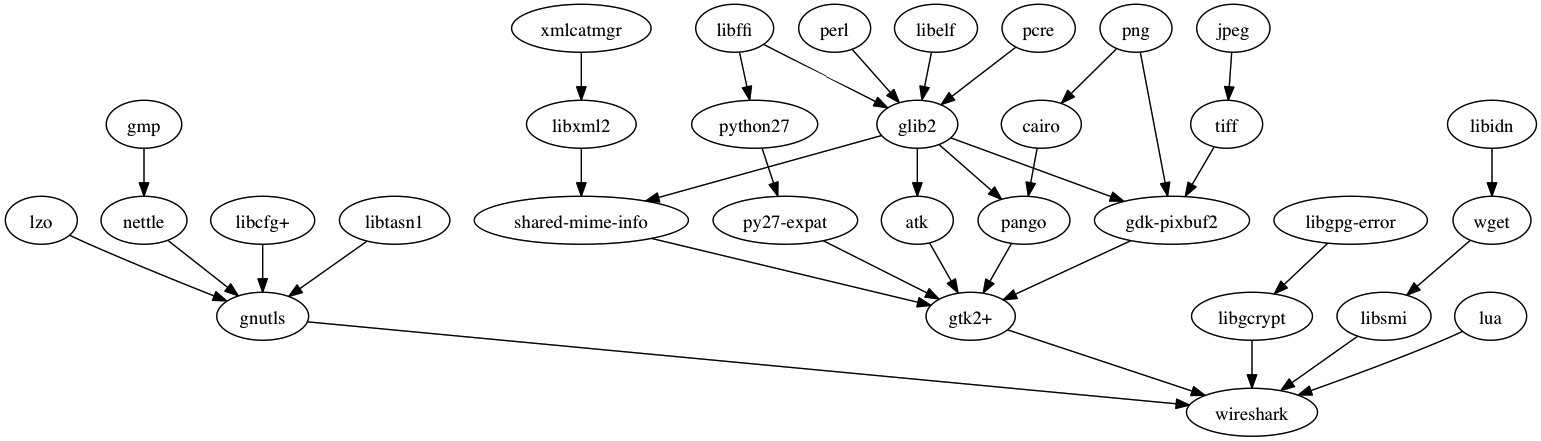
\includegraphics[width=0.95\textwidth]{05/pics/wireshark-dependencies}
		\caption[Software Dependency Tree]{Dependency graph for
			the ``Wireshark'' package, a popular network
			protocol analyzer.
			Package management systems help track such
			intricate dependencies.
			\label{fig:os-installation:wireshark}}
\end{figure}


\begin{itemize}
	\item {\bf Easy package installation.} The most obvious and
		frequent use of the package manager is to install
		software.  These tools usually allow you to only specify a
		name, and they will fetch all required files (including
		pre-requisites) from the Internet, your intranet, or a
		local storage medium and install all the files with the
		right permissions in the right places.

	\item {\bf Automatic resolution of software dependencies.}
		\index{Software!Dependency Tree of}
		Most software relies on specific libraries to be present
		on a system in order to run.  Sometimes the requirements
		are restricted to an operating system, a kernel version or
		another core system component, but more often than not a
		piece of software requires you to install other packages
		in order to be able to use it.

		These software dependencies quickly grow complex: consider
		the requirements expressed in the graph shown in Figure
		\ref{fig:os-installation:wireshark}: in order to be able to
		use a single piece of software, thirty (!) other components
		needed to be installed.  Updating any one of these could
		lead to problems further down in the graph -- and this is
		only a subgraph of the entire system's dependency tree!

		Package management systems keep track of these
		dependencies and allow you to automatically add
		pre-requisite software packages as well as prevent you
		from accidentally removing a component relied on by other
		packages.

	\item {\bf Package inventory.}  As software is installed, the
		package manager keeps track of which packages are added,
		allowing you to get a full list of all software names and
		version numbers in use on any given host.  This, in turn,
		makes it easy for you to identify any required updates, as
		package managers allow you to check whether or not newer
		versions of any given package might be available.

		Some systems even integrate security checks: by comparing
		the list of installed packages to one or more lists of publicly
		known software vulnerabilities, you can get alerted when
		an exploit affecting your hosts has been announced.  Even
		if a fix has not yet been released, this information is
		invaluable, as often you are able to take other measures
		to mitigate the risk.

	\item {\bf File inventory.}  One of the most essential properties
		of any package manager is that it tracks which files belong
		to which package, allowing you to to easily identify the
		purpose of any file or to at least lead you to more
		information about it.

	\item {\bf File integrity.}  Since the package manager already
		maintains a file inventory, it is trivial to also track
		checksums for all files that are installed -- in fact,
		most already do.  This can be used as the basis for a
		simple host-based intrusion detection system.

	\item {\bf Security.}  By downloading source
		code and compiling it on your systems, you are
		inherently trusting the sites from which you retrieve
		the code as well as the transport mechanisms by which
		you did retrieve them.  You are implicitly trusting
		the remote code repository and access restrictions on
		those systems.  That is, you win no security
		assurances unless you manually audit all code paths
		and all dependencies.  This is simply not practical.
		Using signed binaries or packages
		provided by the software project maintainers overcomes
		many of the issues here.

		(It is no coincidence that this last bullet point
		reflects the security concerns we noted in the
		previous section.)

\end{itemize}

\begin{lstlisting}[float,label=code:rpm,caption={[{\em
rpm}/{\em yum} sample commands]Example invocations of
the {\em rpm}/{\em yum} package manager to add a
package, list its files and identify the name of a
package a given file belongs to.}]
$ sudo yum install screen
Password:
Setting up Install Process
Resolving Dependencies
[...]
Updated:
  screen.x86_64 0:4.0.3-16.el6

Complete!
$ rpm -ql screen
/etc/pam.d/screen
/etc/screenrc
/usr/bin/screen
[...]
$ rpm -qf /usr/share/man/man1/screen.1.gz
screen-4.0.3-16.el6.x86_64
$ 
\end{lstlisting}


By using a package management solution, we can build a
central software inventory, which we can then map to a
host's function.  By defining conceptual roles a host
may perform, the software (and in particular what
versions of the given software) to be installed
becomes a configuration option that can easily change
at runtime.  This in turn gives us significant
advantages in our three desired key areas:
scalability, simplicity, and security.  In order to
ensure system consistency across large numbers of
hosts, we can more easily integrate binary packages
into our service inventory and deployment system
(``hosts functioning as web servers will get the {\tt
apache-2.4.3}\index{\tt apache} package installed'') and software
upgrades or patches can consistently be applied using
the same set of tools; we significantly simplify
virtually all operations that require a lookup of what
files are present on which hosts, what version of what
software is running at a given time and how to perform
upgrades with both simple or complex dependencies; by
tracking all software versions and the files the
packages contain, we can easily check for known
vulnerabilities and quickly patch the software.

\begin{lstlisting}[float,label=code:pkg_add,caption={[{\em
pkgrsc} sample commands]Example invocations of the
{\em pkgsrc} package manager and related tools to
visualize package dependencies.  Figure
\ref{fig:os-installation:wireshark} was created using
these commands.}]
$ pkg_add wireshark pkgdepgraph graphviz
$ pkg_info -n wireshark
Information for wireshark-1.8.3:

Requires:
gtk2+>=2.24.12nb3
glib2>=2.32.4nb1
pcre>=8.30nb1
lua>=5.1.4nb1
libsmi>=0.4.5nb1
libgcrypt>=1.4.6nb2
gnutls>=3.0.17

$ pkgdepgraph -S ++wireshark | \
        dot -Tpng > wireshark-dependencies.png
\end{lstlisting}

None of this is possible without the use of a package
management system, but these benefits come with a
price: the packaging system must be used consistently
for {\em all} software.  The act of adding a piece of
software outside this mechanism opens up the
possibility for a broken dependency graph and often
triggers future ``forced'' installations of packages
(i.e. overriding warnings about unmet dependencies,
since the packaging system has no way of knowing what
we installed outside of its catalog) and finally the
loss of a coherent inventory.

Hence it is crucial to be consistent and perform the
at times tedious and frustrating work of
(re-)packaging software in the format that best
integrates with your deployment and management
solutions.  This gets increasingly difficult, as
individual programming languages nowadays come with
multiple (!) language-specific package managers of
their own (see Figure
\ref{fig:software-installation:pip-bower}), as each
language develops its own ecosystem of software
components that their creators cannot provide for {\em
all} possible package managers.

Finally, need to make sure to {\em also} build
packages for all of the software that we do not
retrieve from other sources, for our own software.
That is, when we build software, we have to package it
up and integrate it into our software inventory.  As
we will see in Chapter
\ref{chap:building-scalable-tools}, system
administrators write a {\em lot} of software: we write
small and simple tools just as we write large and
complex infrastructure components; all of these need
to be installed, updated, maintained.  Our own
software is no different from software provided by
others, and so we owe it to ourselves to package it
properly as well.

\begin{figure}[t]
	\centering
	\subfloat[What's pip?]{\label{fig:software-installation:pip}
				\raisebox{.5em}{
					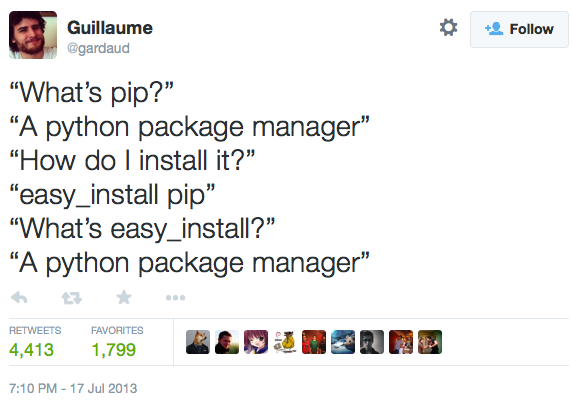
\includegraphics[width=.45\textwidth]{05/pics/pip}}}
	\hspace{1em}
	\subfloat[What is bower?]{\label{fig:software-installation:bower}
				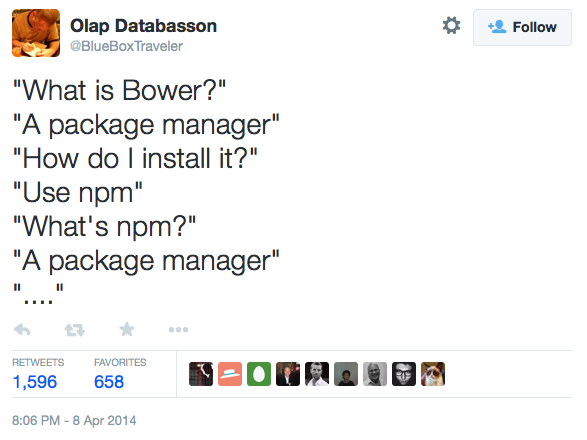
\includegraphics[width=.45\textwidth]{05/pics/bower}}
	\caption{Screengrabs of tweets illustrating the
		circular dependencies of language-specific package
		managers ca. 2014.\label{fig:software-installation:pip-bower}}
\end{figure}



\subsection{Inherent Security Risks}
\label{software-installation:package-management:security-risks}

When we install any software, no matter which method
we use, we are exposing our system to the risk of a
software Trojan, the accidental installation of a
backdoor, a piece of malware\index{malware}.  In an
ideal world, we would verify the integrity of the
software and review what it does, what resources it
utilizes and what information it accesses, receives or
sends.  Unfortunately, doing this for all the software
we download and install is simply not possible, and so
we routinely fetch code from the Internet, compile it
and install the resulting executable.

When we perform these steps, we trust that the code we
are about to install is not malicious because... well,
we just assume that if it was, surely somebody else
would have noticed.  And besides, the website we
downloaded it from looked rather nice, too.  But
suppose that even if we knew that the software we want
to download is not malicious, how do we know that we
are in fact getting it from the website that we {\em
think} it's coming from?

In theory, we can ensure the integrity of the download
by only using secure transport mechanisms (over TLS,
for example) and by verifying a checksum published on
the website in question after the download.  In
practice, doing this work does, once again, not scale:
there simply is too much software released without any
such information.  Fortunately for us, a good package
manager can help in this area, too!

The build process for most software package management
systems ultimately requires a human to decide what
sources to build the software from, and so we are,
when using the resulting binary packages, shifting our
trust from the software provider to the software {\em
package} provider.  Often, these two are the same
person or within the same organizations, but in some
cases, the party providing the package is not the
owner or developer of the software in question.  Just
think of the thousands of RPM or Debian packages
provided by RedHat\index{RedHat} or
Ubuntu\index{Ubuntu}, or the software re-packaged by
the FreeBSD {\em ports} or NetBSD {\em pkgsrc}
systems.

What's more, all software package management systems
need to be able to not only install files, but to run
certain commands required for the proper installation
and configuration of the software in question.  To
this end, they provide the capability for a given
package to execute an arbitrary shell script provided
in the package, with the privileges of the invoking
using -- commonly the superuser.

In other words, it is important to understand that any
time we use a package manager to retrieve and install
software for us from the Internet, we effectively let
it fetch and execute unknown code on our systems.
That is, not only do we trust the package manager
locally -- as well as the software author(s) -- we {\em
also} (and implicitly) trust the people who run and
maintain the package repositories.  These repositories
are managed by system administrators like ourselves --
mere mortals, as highly as we may think of ourselves
-- and every once in a while mistakes are made, and
accounts are compromised, putting at risk users of the
software hosted there worldwide.\footnote{In 2003, the
\gls{gnu} Project's primary FTP server was
compromised.  The possible impact of this is
staggering, given the number of projects that are
relying on the software provided there.  During the
clean-up after the event, every software package had
to painstakingly be verified against known good
checksums, which in many cases were missing and had to
be first identified from other sources.}

Then what is the solution to this problem?  Well,
unfortunately there simply isn't a solution.  We can
build more and more complex systems that provide
better authenticity and better assurance of integrity,
but at the end of the day, we still have to place
trust into systems built and maintained by others.
Ken Thompson's \index[names]{Thompson, Ken} Turing award
acceptance speech ``Reflections on Trusting
Trust''\cite{thompson:trust} cannot remain unmentioned
in this context.  If you are not familiar with this
short paper, look it up on the Internet -- it's
Zen-like moral will change how you regard system
security.

Despite our having to trust so many components outside
our control, and despite the fact that we cannot
eliminate all risks involved, it is important that we
are aware of them.  A good package manager will
provide you with reasonable options to automatically
determine updates from trusted sources and optionally
even apply them.  This requires a significant reliance
on the trustworthiness of the package manager, and
only when we understand the risks can we make informed
decisions.  Perhaps we'll be even a little bit more
careful and observant about how and where our package
management system retrieves its data from or what
other resources we allow it to use.

\section{Managing Software Updates and Patches}
\label{software-installation:managing-updates}

Despite the security concerns, we have praised package
management systems in the previous section as a
reasonable solution to many problems.  Unfortunately,
updating software remains fundamentally difficult and
carries significant risk.  Every time you change a
system component, you are introducing new elements
into your environment and the probability of
unexpected side-effects increases the larger the
change set is.

``If it ain't broke, don't fix it.''\index[names]{Lance, Bert}
has become many a system administrator's mantra,
meaning that unless you have a {\em very} good reason
to change something on a system that is currently
running and not experiencing any problems, you
shouldn't do so.  This simple lesson needs to be
learned over and over again by every system
administrator, and it appears it cannot be learned
without a modicum of self-inflicted
pain.\footnote{Part of this lesson is to understand
that a security problem may very well require us to
judge the software as ``broken'' as any functional bug
or a decrease in usability.}

At the same time, we require agility and high
confidence in our ability to apply significant
changes, to perform package and OS upgrades on a
regular basis.  These conflicting goals -- stability
and agility -- will be part of our discussion of
managing system services in Chapter
\ref{chap:services}. \\

The benefit of a package manager's dependency
resolution has the often undesired result that a
number of pre-requisites or dependencies further down
the graph need to also be updated when a simple
software change to a single package was desired.
Therefore, {\em all} software updates need to be
treated with great care.

The conservative stance hence remains to leave your
system running as is instead of chasing every new
software release, every minor OS update or even to not
bother applying patches if a software vulnerability
appears to not directly impact you.  Unfortunately,
this will make it the more likely that {\em when} an
upgrade finally is required, it will pull with it a
significant number of other changes.  There is no
one-size-fits-all solution to this problem; every
system administrator has to make these decisions for
themselves according to their specific environment.
Until experience allows you to confidently make this
call, it is probably wise to consider any known
security issue to at least warrant very careful
analysis of the possible impact.  \\

When evaluating the need to upgrade a piece of software, it is important
to consider a number of factors:

\begin{itemize}

	\item {\bf Be aware of software updates.}  In order to be able to
		judge whether or not your software needs to be updated,
		you first need to know when new releases are available and
		what features they might include.  Most operating systems
		provide a channel with regular information about release
		updates -- make sure to subscribe to these.  Likewise, you
		probably should track the development process of all your
		major infrastructure components or important products
		(inside or outside your organization).

	\item {\bf Track security updates and announcements.}  Your
		software provider (OS or otherwise) is likely to have a
		mailing list or other information channel dedicated to
		security updates for their software.  You should follow
		these and make sure to evaluate all updates with
		particular attention.

		In addition, you should subscribe to some of the
		mailing lists where vendor-neutral public security
		announcements are posted.\footnote{The ``Bugtraq'' and ``Full
		Disclosure'' mailing lists are two examples.  Searching
		the Internet for these terms should quickly yield the
		right results.} It is not uncommon to first hear about a
		vulnerability for one piece of software here, only to
		find out later on that it also applies to other variations
		you might be running.

	\item {\bf Consider privilege escalation possibilities.}
		Sometimes there are vulnerabilities that do not seem to
		apply to your specific environment, but that can become
		severe when combined with another low-risk vulnerability.
		Make sure to consider all aspects of how your systems
		might be accessed or used when assessing the severity of
		any known vulnerability in the software that you run.
		(We will cover this in more detail in chapter
		\ref{chap:security}.)

	\item {\bf Consider the impact of updating {\em shared
		libraries}.}  The benefit of using shared libraries (no
		need to update all software components using these
		libraries) can become a drawback when a widely used
		library needs to be updated.  As much as software
		providers attempt to provide backwards compatibility,
		sometimes it is (intentionally or coincidentally) broken.
		Software using this library may suddenly start to behave
		erratic or completely stop to function.  Other upgrades
		may even be known to break certain dependent systems.

		It is important to test your software upgrades to ensure
		at least the most basic compatibility is preserved, but
		since it is impossible to exercise all possible code
		paths, you should also weigh the possible impact the
		upgrade may have against the benefits provided by the
		upgrade.

	\item {\bf Consider the impact of updating
		{\em static libraries}.}  This may generally be
		thought of as a less frequent use case, but some
		components may be provided to you or installed on your
		systems using statically linked libraries.  However,
		in the last couple of years (between 2012 and 2017),
		we have seen a tremendous influx of the use of the
		``Go'' programming language (which produces statically
		linked binaries) as well as -- effectively -- by way
		of containers. Here, the update of a package providing
		the library has no effect on the applications using
		this library or the software running inside a
		container -- in order for the change to take effect,
		these applications would need to be re-linked, the
		containers to be restarted.

	\item {\bf Restart applications after the software update.}  In
		order to ensure that all updates have actually taken
		effect, it is usually necessary to restart at least the
		application(s) in question, if not reboot the entire
		system (such as in the case of a kernel or core library
		upgrade).  This implies a service disruption of anywhere
		from a few seconds to several minutes or even longer.
		\footnote{This brings with it the problem of system-wide atomicity
		of software upgrades: it is generally not advised to run a
		given service using different versions of their software
		across multiple systems.  Upgrading all hosts at the same
		time, however, carries the risk of breaking functionality
		(not to mention overall service down time).  Deploying
		such upgrades in a controlled manner across large numbers
		of systems is beyond the scope of this chapter; in fact,
		it easily warrants an entire book by itself.  We'll scratch
		that surface in Chapter \ref{chap:services}.}

	\item {\bf Verify the integrity of your updates.}  When you
		receive software updates, it is important to verify that
		they are in fact updates provided by your provider.  Most
		software distributors cryptographically sign all their releases
		(including software patches), making it easy for you to
		check the integrity of the update.

		Similarly, and depending on the scale of your
		organization, your own infrastructure tools used to roll
		out updates should automatically check all software
		updates in this manner.

	\item {\bf Create your own patches.}  At times, you will find
		yourself in a situation where you need to update a piece
		of software, but the provider has not (yet) released a
		patch.  In some cases you may be able to avoid the problem
		at hand by removing or restricting certain functionality;
		other times, you may be able to fix the problem yourself.

		If you are able to create a patch for a given
		vulnerability, to add a desired feature, or to merge
		another update from a different source, please consider
		contributing it back to both the original software
		creators, as well as to the general public community
		around the software.  Others will surely appreciate this
		help!
\end{itemize}

As you can tell, the above considerations suggest that
determining when, or even {\em if}, you can upgrade
software is far from easy and requires an intimate
understanding of all the details of the running
system.  Even though you can automate the updates of
your software across even hundreds of thousands of
hosts, you cannot automate making the decision to
upgrade.  As a system administrator, this burden is on
you.


\section{Conclusions}
\label{software-installation:conclusions}

In this chapter we have taken a closer look at how
software is installed on a system.  As we reviewed the
boot process, we distinguished between different types
of software, and identified a few distinct categories:
firmware and device drivers, the kernel managing all
hardware and interfacing with the drivers, a number of
core system components such as essential system tools
and libraries, basic applications and utilities
required to make the system usable, and finally
entirely optional add-on applications.  The
distinction between these categories has proven to be
difficult to make, which is why we have further
divided types of software by their place in the file
system hierarchy into the four categories of being
``shareable'', ``unshareable'', ``static'' or
``variable''.

We have looked at the steps required to install an
operating system and discussed the need for a package
management solution to keep track of all files on the
system, as well as the implications of any required
software upgrades.  A package management system, a
requirement for addressing a number of problems when
maintaining large systems with many pieces of software
installed, does not come without its price, however.
As we have stressed, it is important to make {\em
consistent} use of the chosen package manager, but
this has become increasingly difficult: on the one
hand, configuration management tools are able to
manipulate files ``owned'' by the package management
system; on the other, not all software you need to
install is available in the given format.

Building your own packages from sources is laborsome.
What's more, it can be frustrating, as you are
duplicating work already done by others to some
extent.  This holds especially true with respect to
many programming languages and the many smaller
components or modules available for them.  Almost
every modern programming language nowadays includes
its own preferred way of installing language modules
(including the search for and retrieval of the
``right'' version from an online repository).  There
is an old joke in which people lamenting the existence
of too many competing standards get together to create
the one true solution only to end up with just one
more competing standard with limited adoption.  We can
see this holding painfully true when we look at how
different language developers have all solved the same
set of problems (slightly) differently:

Perl has used its {\tt CPAN}\index{CPAN}
infrastructure for decades; Python uses its {\tt
pip}\index{pip} installer; software written in the
Ruby language is often provided as so-called
``gems''\index{RubyGems}; Node.js uses its own package
manager, called {\tt npm}\index{npm}; PHP applications
or extensions are distributed using the {\tt PEAR}
framework and so on.  Each of these tools allows a
package to easily express its requirements on other
language components, but none of these integrates
really flawlessly with other, non language-specific
package managers. (See again Figure
\ref{fig:software-installation:pip-bower}  People
using the RedHat Package Manager (RPM)\index{RPM}, for
example, end up having to re-packaging these modules
or risk breaking their package consistency model.

Others choose to let yet another tool control the
deployment of their software: more than once did we
have to note that defining what software packages or
versions need to be installed on a system is not a
one-time act performed at OS installation time.
Instead, controlling what software is added or
removed, updated, activated or in other ways
manipulated is part of an ongoing process and easily
becomes part of the larger topic of Configuration
Management\index{Configuration Management}.  In fact,
many configuration management solutions -- systems
that apply software configuration changes at runtime
-- include functionality to either require software
packages to be present or are even able to install
them as needed.  We will revisit some of these aspects
in coming chapters.

\vfill
\pagebreak

\chapter*{Problems and Exercises}
\addcontentsline{toc}{chapter}{Problems and Exercises}
\section*{Problems}
\addcontentsline{toc}{section}{Problems}

\begin{enumerate}
\item
Observe the boot process of various systems in your environment.  What
kind of firmware, boot loaders and system software is involved?  Do you
have different boot options leading to a running system with a different
kernel or support for different features?

\item
Review the manual pages (and/or other documentation) of the boot loader(s)
used in your environment.  How hard or easy is it to modify the boot
process?

\item
Review the {\tt hier(7)} manual page on your preferred Unix version.
Identify which components are specifically designated for single- and
which for multi-user operations of the system.  Does the manual page hint
at a separation between shareable and unshareable, static and variable
data?  Compare to two other Unix systems.

\item
Cross-reference the examples in Table
\ref{table:software-installation:shareable-variable} to your system's
manual page or build your own matrix to help yourself identify how the
traditional Unix file system hierarchy applies this model.  Identify three
directories for each combination.

\item
Considering file system and OS implications, identify the hardware and
software requirements for each of the following systems.  Research and
compare common performance requirements and real world use cases to your
suggested solutions.

\begin{enumerate}
\item
a number of web servers, able to efficiently serve tens of GB of small
static files

\item
a number of web servers, able to efficiently serve dynamic content (using
any of the various popular languages and frameworks, such as PHP, Ruby on
Rails, Scala, ...)

\item
a central server hosting a source code repository (very large amounts of
small files with frequent changes, requiring lots of fast I/O and high
data redundancy requirements)

\item
a general purpose workstation / desktop system
\end{enumerate}

\item
\label{prob:software-installation:os-installation}
Perform a basic OS installation of your Unix flavor of choice on a hard
drive (or in an emulator on a disk image).  Note the default values chosen
by the OS, such as partitioning schema, file system choice, number of
packages installed, services enabled and user accounts created.  What type
of system is the OS optimized for?  Do the default installation choices
make this OS more or less suitable for any specific use case?  Consider
the use of the system as a desktop system, a scientific work station, and
a generic Internet facing server.

\item
\label{prob:software-installation:os-installation:manual}
Perform a basic OS installation of your Unix flavor of choice on a hard
drive (or in an emulator on a disk image) without using the OS provided
installer.  That is, perform the steps needed to install an OS on a disk:
partition the hard drive, create a new file system, install a boot loader,
extract the basic OS sets or install the basic OS packages onto the new
disk, add user accounts as needed, enable system services as needed, etc.

\item
Identify the package manager running on your systems and make yourself
familiar with it.

\begin{enumerate}
\item
List all packages installed on your system with version numbers.  Identify
packages that have other packages depend on them as well as ``leaf'' packages
(those without any other package depending on them).  Which package has
the most dependencies, which one is the most depended-upon?

\item
What are the commands to install a piece of software?  To delete a
package?  To upgrade a package?  To downgrade a package?

\item
What are the commands to list the files installed by a given package?
Given a file name, how do you identify what package it belongs to?
\end{enumerate}

\item
\label{prob:software-installation:pkg-vs-manual}
Create virtual OS instances of a few different operating systems, such as
NetBSD, FreeBSD, different Linux versions, and Solaris.

\begin{enumerate}
\item
Compare their default installations.  What kind of packages are installed
on each system?  What kind of services are enabled by default?

\item
Using their default package management system, install the latest versions
of the following software: gcc, perl, python, gnupg, screen, sudo.  How
does the software installation procedure differ?  How can you upgrade or
remove the software?

\item
Using the {\em pkgsrc} cross platform package manager, again install the
same software into a different prefix.  How does the software installation
procedure differ from the native package manager?  How does it differ
across the different systems?  How can you upgrade or remove the software?

\item
Download the source for the same software from their respective
repositories and install it a third time, this time using no package
manager at all.  That is, follow the installation instructions found in
the software package, possibly using the common {\tt ./configure; make;
sudo make install} sequence.  How does the software installation
procedure differ across the various systems?  How can you upgrade or
remove the software?
\end{enumerate}

\item
\label{prob:software-installation:build-a-package}
Identify a piece of software you commonly use, but that is not packaged
for your primary platform.  Create a package for it, then contribute your
changes back to the original author(s) of the software.

\item
All package management systems have certain drawbacks.  Eventually, a lot
of people conclude that the only solution to their problems is to write
their own.  Regardless of the correctness of this conclusion, let us
assume you are in this position.  How would you design a package manager?
Write down the hard requirements it needs to meet, the challenges it needs
to overcome, and identify any optional features.

\item
Review a recently identified security vulnerability in a popular piece of
software.  How were the patches or updates made available?  Can you verify
their authenticity and integrity?

\end{enumerate}

\pagebreak

\bibliographystyle{plainnat}
\begin{thebibliography}{99}

\bibitem{software:silberschatz}Abram Silberschatz, Greg Gagne, Peter B.
Galvin {\em Operating System Concepts}, John Wiley \& Sons, 2011

\bibitem{fhs}Daniel Quinlan, Paul Russell, Christopher Yeoh (Editors) {\em
Filesystem Hierarchy Standard}, Filesystem Hierarchy Standard Group
{\url http://www.pathname.com/fhs/pub/fhs-2.3.html} (visited November 13,
2012)

\bibitem{nemeth:unix-handbook}Evi Nemeth, Garth Snyder, Trent R. Hein, Ben
Whaley {\em UNIX and Linux System Administration Handbook}, 4th Edition,
Prentice Hall, 2010

\bibitem{thompson:trust}Ken Thompson {\em Reflections on Trusting Trust},
Communication of the ACM, Vol. 27, No. 8, August 1984, Association for
Computing Machinery, Inc.; also available on the Internet at
{\url http://cm.bell-labs.com/who/ken/trust.html}
(visited December 5th, 2012)

\end{thebibliography}

\chapter{Of Users and Groups}
\label{chap:multi-user}

\begin{quote}

{\em We trust you have received the usual lecture from
the local System Administrator. It usually boils down
to these three things:\\
\#1) Respect the privacy of others.\\
\#2) Think before you type.\\
\#3) With great power comes great responsibility.} \\
-- Output of {\tt sudo(8)} upon first invocation.
\end{quote}

% XXX add graphic
%\begin{figure}[hb]
	%\raggedleft
	%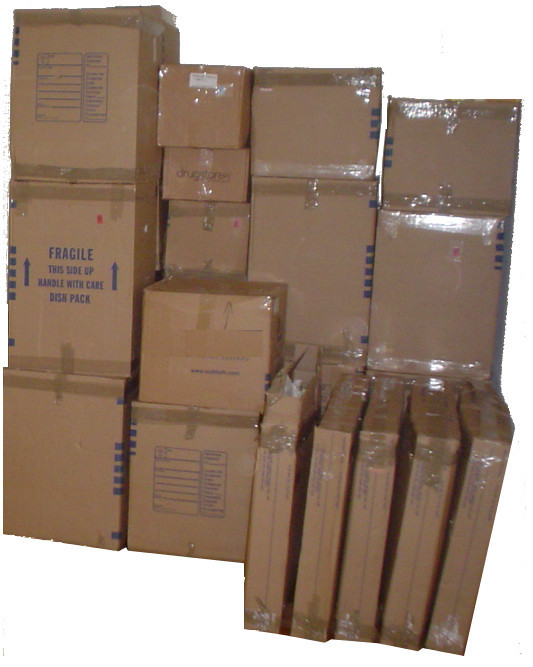
\includegraphics[width=.25\textwidth]{05/pics/many-boxes}
%\end{figure}

\section{Introduction}
\label{multi-user:introduction}

As was noted in Section \ref{unix:basics:multi}, Unix
was designed as a multi-tasking, {\em multi-user}
system, allowing simultaneous access by different
people.  This concept, also found in all of today's
mainstream operating systems as well, demands
important safeguards to prevent both accidental as
well as intentional (i.e. malicious) access by
unauthorized parties.  Since this property affects
virtually all aspects of system administration --
ranging from account management to the way different
software components interact with one another -- it is
important to fully understand the implications of the
nature of a multi-user system.

In this chapter, we will discuss the different types
of users and groups as well as talk about user
authentication on our systems.  Note that even though
there are many parallels to authentication by remote
clients against a service we may offer (such as users
logging into our website), in this chapter we restrict
ourselves to the ``local'' systems and how we access
them internally.

Even if you are comfortable with the Unix multi-user
model, you may still find that explicitly identifying
its inherent requirements and trust models will help
in formalizing your access control requirements so
as to express and apply them using your configuration
management system\index{Configuration Management}, as
we will discuss in the Chapter
\ref{chap:configuration-management}.

As one of our Pillars of Exceptional System Design,
the topic of security weaves through this book like a
red thread, and multi-user principles and the
implications of different access- and trust levels
necessitate a look ahead at topics and ideas discussed
in more detail in Chapter
\ref{sec:security:authn-authz}.  Hence, discussing
the core concepts of {\em
authentication}\index{authentication} and {\em
authorization}\index{authorization} is a natural
requirement and we will attempt to broadly cover them
in this chapter as well.  But let's not get ahead of
ourselves.


\section{Types of Users}
\label{multi-user:types}
\index{Accounts, Types of}

Allowing more than one person access to the resources
of a system requires the computer to be able to {\em
distinguish} between different users, which of course
is done by providing distinct {\em user accounts}.
When a user wishes to use the system, she identifies
herself to the computer (for example by entering her
login name), upon which the system authenticates her
(for example by prompting her for a password). Upon
successful authentication, she is then granted access
to her files and/or is allowed to run certain
programs.  But this simple association of human beings
to computer accounts -- in the Unix world implemented
using numeric {\em user-IDs} -- does not paint a
complete picture.

It is easy to assume that different ``users'' refer to
distinct people accessing the resources, and ideally
we'd want to keep the mapping between the two sets
(``persons'', ``accounts'') to be of a 1-to-1 (and
{\em onto}) nature.  But we quickly run into problems:

On a typical Unix system, you will find a perhaps
surprising number of accounts that are {\em not}
associated with actual human beings at all. To
illustrate this, Listing \ref{code:cat-passwd}
displays excerpts of the standard Unix password
database, the {\tt /etc/passwd} file, on a NetBSD
system.  Reviewing the first few rows, we find most of
them reference so-called {\em system
accounts}\index{Accounts, System}, present to allow
specific services to run with only the permissions
they need, a concept known as privilege
separation\index{privilege separation} or the
{\em Principle of Least Privilege}\index{Least Privilege,
Principle of}. This ensures, for example, that a
software error in one d\ae mon cannot accidentally
lead to access or deletion of files owned by another
user.

\begin{lstlisting}[float,label=code:cat-passwd,caption={Excerpt of a
typical {\tt /etc/passwd} file on a NetBSD system\index{\tt apache}}]
root:*:0:0:Charlie &:/root:/bin/csh
toor:*:0:0:Bourne-again Superuser:/root:/bin/sh
daemon:*:1:1:The devil himself:/:/sbin/nologin
bin:*:3:7:Binaries Commands and Source:/:/sbin/nologin
postfix:*:12:12:& pseudo-user:/var/spool/postfix:/sbin/nologin
named:*:14:14:& pseudo-user:/var/chroot/named:/sbin/nologin
ntpd:*:15:15:& pseudo-user:/var/chroot/ntpd:/sbin/nologin
sshd:*:16:16:& pseudo-user:/var/chroot/sshd:/sbin/nologin
_pflogd:*:18:18:& pseudo-user:/var/chroot/pflogd:/sbin/nologin
nobody:*:32767:39:Unprivileged user:/nonexistent:/sbin/nologin
www:*:1003:1000:apache www user:/nonexistent:/sbin/nologin
spamd:*:1004:1001:Spamd User:/var/chroot/spamd:/sbin/nologin
deploy:*:1234:1234:& User:/var/app:/usr/local/bin/app-update
jschauma:*:1000:100:Jan Schaumann:/home/jschauma:/bin/ksh
alice:*:1001:100:Vincent Damon Furnier:/home/alice:/bin/ksh
bob:*:1007:100:Nesta Robert Marley:/home/bob:/bin/sh
\end{lstlisting}

In addition to these system accounts, we also
frequently find what has become to be known as {\em
role accounts}\index{Accounts, Role}: accounts that,
while not specifically tied to a single person, are
used to allow multiple people to initiate certain
well-defined actions.  A common example is a role
account to allow for automated updates to a given
service or application. \\

In order to manage the resources to be made available
to different users, to control the system, to add or
remove software etc., we require the use of an
omnipotent account, known as the
superuser\index{superuser}.  This account is commonly
called the {\tt root} account, and is identified by
the numeric user-ID 0.\footnote{As user privileges
on a Unix system are only identified by the {\em
effective user-ID} of a given process, the system does
not care one bit whether or not the string mapped to
the UID 0 happens to be ``root'' or ``bob'' or
``susan''. That is, superuser accounts with other
names are entirely possible; ``root'' just happens to
be one of those old Unix conventions we've all grown
so accustomed to.  It is good practice -- and part of
most standard security scans -- to periodically check
for the existence of ``other'' accounts with UID 0.}
In order to gain superuser privileges, a user needs to
either log in as {\tt root}, assume the superuser's
identity via the {\tt su(1)}\index{\tt su(1)}
command, or make use of, for example, the popular {\tt
sudo(8)}\index{\tt sudo(8)} utility (which also
offers some more fine-grained control over who may
gain what privileges).

\begin{sidenote}
{\bf Of Headless Users and Privilege} \\

{\em Role Accounts} may be known by a variety of
names, depending on the history of the organization:
``service account'', ``headless users'' (because no human is
associated with the account), or, frequently, by the
name of the company or organization.  Now a funny
side-effect of using a service account intended for
privilege separation to automate certain tasks is
that this account becomes more and more powerful with
time: every task it needs to accomplish (such as
installing or updating software, starting or stopping
services, monitoring services or alerting on
conditions) requires the user to have the necessary
privileges. \\ [10pt]

Take a look in your {\tt /etc/passwd} -- if you work
at company ``Gizmo App, Inc.'', chances are the most
powerful user (besides {\tt root}, of course) is
``gizmo'', and {\tt gizmo}'s access credentials are
shared across multiple systems.  We will discuss this
dilemma and some possible ways to mitigate it in
Chapter \ref{chap:security}.
\end{sidenote}


Perhaps somewhat paradoxically -- usually, we wish to
have a unique mapping from exactly one person to
exactly one user-ID -- access to this superuser
account is shared: all system administrators within an
organization need to have this kind of access by
necessity.\footnote{A discussion of the limitations in
the traditional Unix permissions model that make this
shared superuser account a virtual necessity would be
beyond the scope of this chapter.  For completeness's
sake, however, we should mention that more modern
access semantics, such as {\em mandatory access
controls} (MAC), {\em role-based access controls}
(RBAC), or POSIX ``capabilities''  can been added,
albeit at the cost of increased complexity.}

Reviewing these access rules, we can identify mappings
of zero, one or more people to a given account (Figure
\ref{fig:multi-user:mappings}), as well as a single
person with access to multiple accounts.  From the
system's perspective the differences are irrelevant
(all process privileges are granted solely based on
the UID), but as system administrators, we have to
treat each class of users differently.  As a general
rule of thumb, we want to ensure, for example, that
only those accounts used by people have an
interactive login session.  All other accounts should
be restricted such that they can only execute specific
commands or access specific files\footnote{On some
Unix systems, it is possible to restrict a given
process to a specific subset of the file system --
see, for example, the {\tt chroot(8)}\index{\tt
chroot(8)} command.  In the past, assigning a user a
so-called {\em restricted} shell was another method of
limiting what actions a user may perform.}.  This
becomes difficult quickly especially when using role
accounts, as often a certain set of interactive
commands need to be allowed.  Care must be taken to
correctly identify and enforce the restriction to
just these commands.

If you look closely at the example password file shown
in Listing \ref{code:cat-passwd}, you may notice that
in addition to the {\tt root} account there is a
second account with UID 0, called {\tt toor}. This
account, often found on the BSD derived Unix variants,
does in fact offer a second superuser account: it is
usually given a different login shell to provide for a
way to repair the system in case {\tt root} is unable
to log in (for example due to a broken login shell as
a result of a software upgrade).  This illustrates
that it is possible for a Unix system to have multiple
usernames mapping to the same UID, though it should be
noted that generally speaking that is not a good idea
and likely to be an error.

\begin{figure}[!hb]
	\centering
	\subfloat[User mappings]{\label{fig:multi-user:user-mappings}
			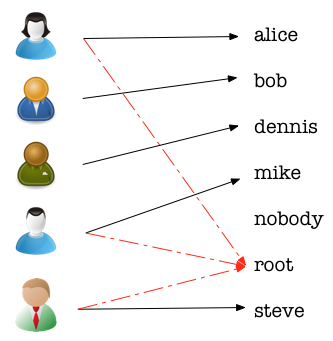
\includegraphics[width=.3\textwidth]{06/pics/user-mapping}}
	\subfloat[Group mappings]{\label{fig:multi-user:goup-mappings}
			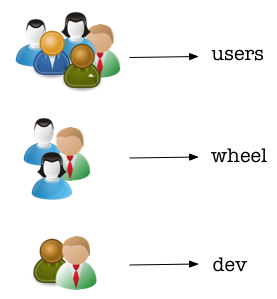
\includegraphics[width=.3\textwidth]{06/pics/user-groups}}
	\subfloat[Groups to machines mappings]{\label{fig:multi-user:goup-machine}
			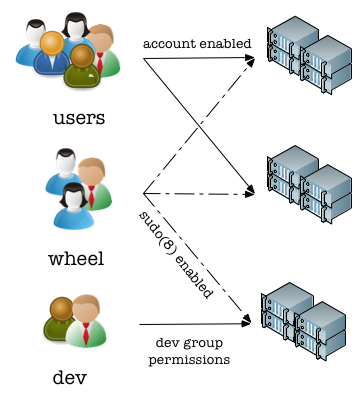
\includegraphics[width=.3\textwidth]{06/pics/groups-machines}}
	\caption[User Mappings]{The set of users mapping to the
			set of account names is neither bijective (or
			``one-to-one''), nor surjective (or ``onto''):
			some accounts are not used by an actual user,
			while others may be used by more than one user.
			Users are associated with local groups on a given
			host, and group membership may imply specific
			privileges across a set of hosts.
			\label{fig:multi-user:mappings}}
\end{figure}



\section{Groups of Users}
\label{multi-user:groups}

In addition to different {\em types} of users, we can
also identify different {\em groups} of users.
Privilege separation is a fundamental best practice in
the area of system administration: every user should
be given exactly the level of access they require,
with elevated or superuser privileges being
particularly strictly controlled.  But even outside
this special group, there are a number of users who
need to share resources with one another.  The nature
of the environment you are in plays an important role
here, as (implicit) trust or lack thereof create
vastly different use cases.  For the purposes of this
discussion, let us define a group of users as a number
of people who are either collaborating in some
capacity -- meaning they will wish to share read and
write access to certain resources -- or require
similar execute privileges, for example to start,
stop, or otherwise control a specific service.

In a small commercial environment, such as a start-up,
the good will and intent to collaborate for all users
of your systems is implied.  In such environments all
users do frequently require the same or at least
similar access to all systems, as responsibilities are
shared and job duties overlap.  As a result, you will
find few distinct groups here, and getting access to
one system tends to simultaneously get you (the same
broad) access to all systems.

As the environment grows in size, however, you will
find that you need to group accounts more carefully.
For example, all developers on a given software
project require access to systems on which to build
the software, write access to the central source
revision control\index{revision control} repository
and the like, and so are grouped together; they do not
require -- nor should they have -- access to the
systems processing credit card payments or which
contain payroll information.

In even larger companies, you may find that groups
sharing access to the same set of servers may have
competing resource requirements, even if we assume
that every user has been given an account for the
ultimate benefit of the organization at large. In
addition, the larger your organization grows and the
more users you have, the higher the risk of any one
account getting compromised becomes.  Recall our
earlier discussion of well-defined and documented
policies in Section
\ref{documentation:types:policies}; it is no surprise
to find a requirement for very specific access
policies, that spell out in detail who should be
granted what level of access on the one hand and for a
complete audit trail of who was given said access on
the other. \\

In contrast to these use cases, now consider the
different groups of users present in an academic
environment, such as a large university.  Access to
computing resources is made available to students,
faculty, staff, and possibly visiting researchers.
Even disregarding any outside compromise, you have at
times almost directly conflicting privacy
requirements: students should not be able to access
faculty resources or files (and yet may have an
explicit interest in doing so!), but students working
as teaching or faculty assistants sometimes should;
student homework assignments done on shared servers
should not prevent research jobs from running; faculty
may collaborate with each other on some projects, with
outside researchers on others.

Finally, if you are maintaining public systems for an
Internet Service Provider (ISP), you may find yourself
trying to manage hundreds or thousands of completely
unrelated user accounts with little to no
collaboration amongst them.


Group definitions exist in every organization, and are
often drawn outside the system administrator's
purview; it is not uncommon for computer systems to
inherit a group structure by mapping the
organization's functional hierarchy into different
user groups.  However, sooner or later you will run
into limitations and require more fine-grained
control.  A careful analysis of the different types of
users, the different groups based on requirements and
needs, and a directory service that allows you to
easily create (possibly intersecting) sets of users
are needed to allow your systems to grow with and
adapt to the needs of whichever type of environment
you are in.  We will get back to this concept of
grouping users and mapping them to similarly grouped
sets of hosts in our next chapter.

\begin{experience}
{\bf All users are equal...} \\

In almost every organization, there are a few users
who have {\tt root} who... shouldn't: there's the
ex-system administrator, who now works in a different
area but who occasionally is called upon when tribal
knowledge from the olden days is required; there's the
competent software developer who always needed special
resources and who finally managed to convince one of
the system administrators to let him have superuser
access to fix his own systems; there's the CEO who
simply ``requires'' superuser access to all machines,
even though the last time he opened a terminal was 10
years ago when he updated the single web server of his
then-fledgling start-up. \\ [10pt]

And then there's the start-up founder, who not only
routinely tinkers with the OS kernel and system
configurations, but oversees the hardware allocation
requests in what has become an Internet giant with
tens of thousands of hosts in data centers across the
globe: \\ [10pt]

While working at Yahoo!, I continually tried to keep
small the number of people whose accounts were
included in the OS images.  As an initially large
number was slowly reduced (often only after many
discussions, assurances of emergency failover
procedures, and arguments), I finally had to tell
David Filo\index[names]{Filo, David} (one of Yahoo!'s
founders) that I intended to remove his account as
well.  After a few discussions, assurances of
emergency failover procedures, and arguments, we
eventually agreed to have it removed from the OS
images, but to let our configuration management
systems add it as necessary.  To the best of my
knowledge, Filo, as he is known to all employees,
still logs into production servers to analyze and
challenge current resource usage whenever engineers
request new hardware, and he still traces and fixes
kernel bugs that require him to have access to most,
if not all, systems.  \\[10pt]

Every system administrator I know has a similar story
to tell; they frequently end with ``Well, he doesn't
{\em need} access, but he's the boss, so...''. \\
[10pt]

{\em Some users are more equal than others.}
\end{experience}

\section{User Authentication}
\label{multi-user:authentication}
\index{authentication}

We mentioned earlier (albeit somewhat tersely) that
the system authenticates the user at login time.
Seeing how this is a rather important aspect of a
multi-user system, let us spend a little bit of time
to make sure we understand what exactly happens.  As
we will discuss in more detail in Chapter
\ref{chap:security}, when we are authenticating a
user, we are ensuring that user is who they claim to
be.  More precisely, we are verifying that whoever is
identifying themselves as user ``alice'' can in fact
provide the credentials which we assume only Alice to
have access to.\footnote{Unlike the system
administrator in charge, the computer does not care if
Alice gives her credentials to Bob and allows him to
log in as her.}

{\em Authentication} (frequently referred to as {\em
AuthN}) is the act of providing a proof of identity,
not a proof of {\em authorization} ({\em AuthZ}).
Although frequently entangled, the former only answers
the question ``Are you really who you say you are?'',
while the latter concerns itself with the question
``Are you allowed to perform this action?''.  There
are many different ways of providing a proof of
authentication; we generally divide them into the
following three classes\footnote{Cynical information
security professionals, always happy to point out
weaknesses in any system, like to refer to these
categories as ``something you forgot, something you
lost, something you stopped being''.}:

\begin{itemize}
	\item {\em something you know}, for example a password
	\item {\em something you have}, for example a
		physical key or a hardware token
	\item {\em something you are}, a biometric
		factor, such as e.g. a fingerprint
\end{itemize}

Each authentication method has its own strengths and
weaknesses, with usability and convenience being
important factors upon the final security they may
provide:  passwords that are easy to remember are also
easy to guess or crack, physical tokens can be lost or
stolen, and biometric factors are near impossible to
replace or change in case of a compromise.

In many cases, it is desirable to combine some of
these authentication methods to yield the desired
level of security and usability.  So-called
``two-factor authentication'' or {\em
2FA}\index{authentication!2FA} has
recently become a popular protection mechanism used by
many internet sites: in order to gain access to a
service, the user needs to provide e.g. a password
({\em something you know}) as well as a code generated
by an app on their smartphone (the phone thus being
{\em something you have}).  It is entirely possible --
and at times desirable -- to add more factors or vary
combinations of factors, which is why the more general
term ``multi-factor
authentication''\index{authentication!multi-factor}
(MFA) is more precise.

Lastly, let us note that even though we frequently
only consider authentication of one party, {\em mutual
authentication}\index{authentication!mutual} is an
often desired or even required property of a secure
system:  when a user logs into a system, the system
wishes to authenticate the user, but the user also
needs to have assurance that the system they are
logging in to is the system they think it is.

\subsection{Authentication Examples}
\label{multi-user:authentication:examples}

To illustrate the many different ways we may use or
encounter authentication in our day to day operations,
let us look at a few examples:

\begin{lstlisting}[float,basicstyle=\scriptsize,label=code:password-login,caption={[Password
authentication on the console]Password authentication
on the system console on a NetBSD server.}]
NetBSD/amd64 (SERVER) (console)

login: jschauma
password: *********************************
NetBSD 7.0.2 (SERVER) #2: Tue Jan 24 02:33:13 EST 2017

Welcome to NetBSD!
hostname$
\end{lstlisting}

Listing \ref{code:password-login} illustrates the most
simple example: password authentication on the system
console of a NetBSD server.  The user provides their
username and password; if the password matches (see
below), the user is logged in.

\begin{lstlisting}[float,basicstyle=\scriptsize,label=code:ssh-login,caption={[SSH
key authentication]An example of mutual authentication
by way of SSH keys.}]
$ ssh -i ~/.ssh/mykey server
The authenticity of host 'server (192.0.2.12)' can't be established.
ECDSA key fingerprint is 19:af:35:01:0b:2a:ee:3d:30:0f:69:11:cc:55:7c:20.
Are you sure you want to continue connecting (yes/no)?  yes
NetBSD 7.0.2 (SERVER) #2: Tue Jan 24 02:33:13 EST 2017

Welcome to NetBSD!
hostname$
\end{lstlisting}

Listing \ref{code:ssh-login} shows another method of
authentication so frequently used that we hardly ever
think about it.  Here, we see asymmetric key
cryptography\index{cryptography!asymmetric} as a means
of authentication, effectively using a {\em something
we have} (a private SSH key).  But note that at the
same time, the server also offers {\em us} a way to
authenticate {\em it}: the SSH hostkey fingerprint
presented on the first connection allows us to verify
that the server is in fact the one we intended to
connect to.  If we know the server's expected hostkey
fingerprint (which itself is derived from the private
hostkey that presumably nobody else would have access
to), then we can compare and match them, thereby
authenticating the server.\footnote{Unfortunately, the
distribution of known hostkey fingerprints and
changing identities in a large scale environment have
lead most people to blindly accept any hostkey
fingerprint presented.  Doing so is an example of {\em
\gls{tofu}}\index{Trust on First Use}.  We will get
back to this problem in later chapters.}

\begin{lstlisting}[float,basicstyle=\scriptsize,label=code:krb-login,caption={[Kerberos authentication]Mutual authentication via a central Kerberos service.}]
$ kinit
Password for jschauma@DOMAIN: ********************************
$ klist
Ticket cache: /tmp/krb5cc_ttypa
     Default principal: jschauma@DOMAIN

     Valid starting     Expires            Service principal
     02/13/17 13:50:21  02/13/17 21:50:20  krbtgt/KDC@DOMAIN
$ ssh somehost
somehost$
\end{lstlisting}

Listing \ref{code:krb-login} illustrates the use of a
central authentication service by way of the
Kerberos\index{Kerberos} protocol.  Here, we are
authenticating ourselves to the central service using
a password ({\em something we know}).  We then use a
time-based token (a ``ticket'' in Kerberos lingo, i.e.
{\em something we (now) have}) to authenticate
ourselves to the server we wish to access.  At the
same time, the Kerberos network authentication
protocol also takes care of authenticating the server
to us.  This setup thus includes multiple
authentication methods as well as an example of mutual
authentication.

\begin{lstlisting}[float,basicstyle=\scriptsize,label=code:sshca-login,caption={[SSHCA
and MFA example]An example of very strong
authentication: the use of a certificate authority,
combined with a password and multiple physical
tokens.}]
localhost$ ssh sshca
YubiKey for `jschauma': ********************************
Password: ********************************
localhost$ ssh-add -l
2048 SHA256:TzwuHGc5BKBe+VJSnGoVyh92J8XKBUkaL7MGQn8ML0Y (RSA)
2048 SHA256:TzwuHGc5BKBe+VJSnGoVyh92J8XKBUkaL7MGQn8ML0Y (RSA-CERT)
localhost$ ssh somehost
Duo two-factor login for jschauma

Enter a passcode or select one of the following options:

 1. Duo Push to XXX-XXX-0712
 2. Phone call to XXX-XXX-0712
 3. SMS passcodes to XXX-XXX-0712

Passcode or option (1-3): 1
Success. Logging you in...
Last login: Thu Jan 26 17:39:30 2017 from 10.1.2.3

somehost$
\end{lstlisting}

Listing \ref{code:sshca-login} finally illustrates the
use of several strong factors combined with time-based
access credentials to form a particularly strong
example of authentication.  Here, we are making use of
a Certificate Authority (CA)\index{certificate
authority} for use with SSH to issue short-lived
access credentials.  In order to receive such a
certificate, the user must first authenticate to the
{\tt sshca} service, which requires both a password
(again: {\em something we know}) as well as a
cryptographic One-Time Password
(OTP)\index{passwords!one-time} generated by a
hardware token ({\em something we have}).  In addition
to the client certificate we received from the CA, the
server we are finally accessing also implements
another form of two-factor authentication, offering to
send a message to the user's cell phone and requiring
an interactive acknowledgement.  If the cell phone in
question requires a fingerprint to unlock, then we are
even adding a biometric factor ({\em something we
are}).  Phew, that is one tough system to access!

\subsection{The Problem with Passwords}
\label{multi-user:authentication:passwords}

Despite the variety of authentication methods
available, password authentication remains the lowest
common denominator and is worth looking at in a little
bit more detail.

More often than not, the credentials used to
authenticate at login time are simply a password of
often pitiful complexity.  Much like you may have not
let your sister (or her friends) climb into your tree
house unless they knew the secret passphrase, the Unix
system will not let you log in without you entering
the correct string of characters.

It is important to understand at this point that the
Unix system does not actually compare the string you
entered to the string it has stored in a database, but
that instead it operates on password {\em hashes}.
That is, the string you entered (together with a few
bits of additional data known as the {\em salt}) is
transformed via a one-way function that produces a
fixed-length string of (different) characters, which
are then stored and compared against at the time of
authentication.  Since this transformation is a {\em
one-way} function, it is impossible for anyone to
reproduce the original password from the hash -- an
important cryptographic property of the function used.
If this password hash matches the one on record,
access is granted, and you are logged in.  From that
moment on, regular Unix semantics and permissions will
apply to decide whether or not access to a given
resources (e.g. the ability to write to a file) is
granted.

Passwords are an easy and convenient way for users to
authenticate to a system.  However, there are quite a
few drawbacks that it is important to be consciously
aware of.

As noted above, we do not actually store clear text
passwords in a database, as this would mean that
anybody (and any process) able to access this database
had access to all users' passwords.  Instead, the
use of a hash ensures that even using a privileged
account, we cannot see the users' clear text
passwords.  Still, we wish to protect the password
hashes from prying eyes, which is why our Unix
systems no longer store them in the world-readable
{\tt /etc/passwd} database, but instead in a separate,
protected file (such as {\tt
/etc/master.passwd}\index{\tt /etc/master.passwd} on
BSD derived systems or {\tt /etc/shadow}\index{\tt
/etc/shadow} on many System V derived Unix
versions).

But, and this is one of the problems when using
passwords for local authentication, this data has to
exist on all the hosts a user wishes to log in on.
That, in turn, means that if a single host in the
environment is compromised, the attacker gets their
hands on {\em all} users' password hashes.  Once
retrieved, they can then perform so-called offline
dictionary attacks on the password hashes or look them
up in widely available {\em rainbow
tables}\index{rainbow tables}, large pre-computed
mappings of common strings to their hashes.

The solutions, or rather, the efforts to at least
partially address these issues include the use of a
password {\em salt}\index{salt}, the previously
mentioned small amount of data added to the user's
password prior to the application of the hash
function, thereby yielding a different hash on
unrelated systems despite the password being the same
and thus defeating simple rainbow table look ups.

Another approach used frequently is to not make the
password hash locally available on each host and
instead rely on an authentication system where the
actual password hashes and additional user
information is stored in a central place and is
accessed over the network.  The {\em
\gls{ldap}\index{LDAP}} is an example of this
approach.  However, it should be noted that the
benefits of a central location of this information
carries a certain prize, as well: if the host(s)
providing this service becomes unavailable, thousands
of hosts can become unusable or see debilitating
errors.  This problem can of course be defined in a
more general statement: as an environment increases in
size, relying on a central service poses an increasing
risk of becoming a {\em Single Point of
Failure}\index{Single Point of Failure} (often
abbreviated as ``\glslink{spof}{SPOF}''), while
distributing data across thousands of servers poses
its own data replication and synchronization
challenges while simultaneously increasing the
probability of it being compromised.

What's more, passwords are an inherently insecure
means of authentication, largely due to human nature:
most people are rather terrible at remembering complex
passwords (which are harder for computers to crack)
and hence tend to use and reuse across different sites
a small set of a simple passwords This means that
accounts on your systems may get compromised by
password leaks in another, completely different and
independent environment!

Many solutions or improvements to this dilemma exist,
ranging from multi-factor authentication protocols to
randomly generated passwords stored and managed by
specific password management tools.  We will discuss
some of these in our chapter on security later in the
book.

\subsection{Sharing {\tt root}}
\label{multi-user:authentication:shared-root}

As noted in Section \ref{multi-user:types}, the {\tt
root} account is commonly shared, meaning multiple
people know the password to authenticate as the
superuser.  This, however, poses a number of problems.
When a system administrator leaves the organization,
the {\tt root} password needs to be changed, all
systems need to be updated with the new password hash,
and the new password has to be communicated to all
members of the team.  Despite many best practices of
sharing or storing shared secrets like this, the more
people who require said access, the larger the risk of
accidental exposure of the password or its hash.

Secondly, since the {\tt root} account is a {\em
system} account, it may not be included in any central
user directory (such as your \gls{ldap} service), and
instead be managed either via your configuration
management system, or your OS image.  This may lead to
the password hash being available in additional
places, such as the configuration management's
repository or the OS image build system.  Again: the
more places such important access credentials are
stored, the more likely it is that they can be
accessed by unauthorized parties.

Finally, by mapping multiple people to a single
account you lose an important audit-trail: no longer
is it possible to identify who performed a given task;
all we can do is identify a (possibly large) group of
people who could have done so.  Given the powers of
the superuser account, this is particularly
bothersome.

It is common best practice to disable logins from {\tt
root} over the network\footnote{It is also possible to
completely disable the {\tt root} account, though that
may have implications on your ability to recover the
system without physical access in the case of a severe
failure.}, requiring users to first log in with their
usual account, and then to use the {\tt
su(1)}\index{\tt su(1)} or {\tt sudo(8)}\index{\tt
sudo(8)} utility to perform certain actions with
elevated privileges. Since this tool logs all
invocations, we nicely solve the problem of the
missing audit trail; in addition, we gain much finer
grained control of what access is given to which
users.

Note, however, that this solution is no panacea: it is
easy to fall into a false sense of security when
restricting superuser privileges to a few explicit
commands while forgetting that many of these commands
allow a skilled user to invoke or otherwise trick the
system into executing other, non-sanctioned
commands.\footnote{Most Unix editors, for example,
allow a user to invoke a shell; dynamically linked
executables can be tricked into loading custom
libraries; the possibilities to exploit access to a
small number of tools running with superuser
privileges are too numerous to account for.}  As a
general rule of thumb, you should consider the use of
{\tt sudo(8)} primarily for its audit-trail
capabilities and only grant its use to trusted users.

Secondly, this approach only works on actual server
operating systems.  Networking equipment, such as
switches, routers, or load balancers, where the {\tt
TACACS+}\index{\tt TACACS+} and {\tt
RADIUS}\index{\tt RADIUS} remote authentication
protocols allow well-defined control of remote access
do, for the most part, still follow an all-or-nothing
access model locally.  The access credentials for the
privileged accounts on these devices (as example might
be the ``enable'' password, used to enter privileged
mode on a router or switch) need to be managed and
shared with the same care that a {\tt root} password
would be.

\section{Summary}
\label{multi-user:summary}

Even though taken for granted nowadays, the nature of
a {\em multi-user} system has had from the beginning a
number of important implications for overall system
security and operational procedures.  The impact of
these implications grows near exponentially as your
environment scales up, which is why we make a point of
identifying them explicitly in this chapter.

Users fall into a number of well-defined categories,
or {\em types} of users.  In particular, we
distinguish for good reasons between user accounts
used by actual humans and so-called system accounts.
Different users (of either kind) have at times
conflicting requirements and impose very specific
trust models on the environment.  Access privileges
need to be defined and enforced, and authentication
methods need to be considered.  We briefly mentioned
passwords as the most common form of authentication
and noted a few of the problems associated with them;
we also covered some of the implications of sharing
{\tt root} access with your peers.

More generally speaking, though, we looked at what it
means for a system to support multiple users.  System
administrators with experience managing deployments in
diverse environments are able to recognize and apply
these general rules:

\begin{itemize}
	\item {\em All users are equal.}  We need to be able to
		accomodate different use cases and equally enable many
		different types of requirements.  All groups of users
		should be treated with the same professionalism and their
		needs appropriately addressed.
	\item {\em Some users are more equal than others.}  While all
		users' needs should be addressed, there are, in any
		system, some users who have more specific requirements;
		who need certain elevated privileges; whose computing
		demands exceed those of others.
	\item {\em All users are to be given precisely the access rights
		they need, but no more.}  The principle of least privilege
		needs to be rigorously applied, as any one account may
		become compromised, and the possible damage deriving from
		this scenario needs to be limited as much as possible.
	\item {\em Trust does not scale.}  When building your
		infrastructure, remember that while you may trust all
		users in your organization {\em today}, you will
		eventually grow to a size where this no longer holds.  It
		is near impossible to later on put in place restrictions
		on users' privileges, just as it is to anticiapate the
		possibly sudden departure of trusted employees.
	\item {\em You will always face tradeoffs.}  No matter which
		authentication mechanism you choose, there are downsides.
		Eliminating single points of failure may increase your
		infrastucture's complexity or increase the risk of
		exposure of confidential information.  (This holds for
		many other aspects of system administration, too, but the
		impact may be most obvious when it comes to
		authentication of users.)
\end{itemize}

When you manage a sufficiently large or diverse group
of systems, you will learn to abstract individual
users (and their requirements) into more conceptual
{\em groups of users}.  These groups may then be
translated to access privileges on a given host, or,
as you scale up your environment, to mappings of
privileges to {\em sets of hosts}.

Controlling only a few hundred machines, it is easy to
think in terms of individual hosts.  However, today's
Internet giants tend to operate by utilizing tens or
hundreds of thousands of hosts.  At this scale,
services are defined not by which individual machines,
but by which {\em datacenter} handles the requests.
Individual hosts become irrelevant, even though access
control, by and large, still follows the same model,
even if operating on a different scale.

Due to this shift in scale, a distinct trend away from
managing user access on an individual host basis and
instead shifting towards a {\em Service
Orchestration}\index{Service Orchestration} model has
formed in the last couple of years.  In this world,
interactive logins to any single host are unnecessary
and imply a systemic failure, as unavailable hosts
should automatically be taken out of a
production-serving rotation and overall load be
distributed to the remaining, working hosts.

Services are run as so-called system accounts
unassociated with actual users.  Nevertheless, regular
multi-user semantics apply.  The principles of how
access to any given resource is granted, how services
(or users) are authenticated, and how a clear
separation of privileges provides the foundation for
overall system security is not different when applied
to user accounts that end up being mapped to humans
versus those that are not.  \\

A multi-user system implies the existence of a
privileged account, which, by necessity, is shared
amongst multiple people.  The fact that this account
is also -- by definition -- a system account embodies
the paradoxical complexity of managing {\em all} user
accounts (whether or not they may be mapped to people
or service roles).  The only way to retain a modicum
of sanity when managing these many-to-many mappings of
privilege in a large environment is a clear definition
of host and user access groups.  As we will see in the
following chapter, creating and operating on these
sets of resources in the abstract is best done using a
configuration management system.

Looking towards the future (as we will in Chapter
\ref{chap:future}) -- and catching up a bit with
developments since I first started writing this
chapter back in 2012 -- we should also note that as
the industry moves further towards more ephemeral
systems, such as through the use of containers and
virtualization technologies, the overall headache of
managing local user accounts may well be a thing of
the past: systems are defined in a descriptive way and
spun up or torn apart as needed.  Nevertheless, as
experienced system administrators, we are well aware
that new headaches may well lie hidden here, and the
{\em concept} of authenticated access by multiple
users (for humans and services alike) continue to
apply.

Thus, the burden of {\em identifying} the proper
access model, however, remains with the system
administrators.  Let's make sure that we understand
the implications of multi-user access on all of our
systems as we do!

\vfill
\pagebreak

\chapter*{Problems and Exercises}
\addcontentsline{toc}{chapter}{Problems and Exercises}
\section*{Problems}
\addcontentsline{toc}{section}{Problems}

\begin{enumerate}

\item Review the {\tt passwd(5)}\index{\tt
passwd(5)} manual page and make sure you understand
what each field is used for.  Is this password
database used on the systems you have access to, or is
authentication done by way of a central system, for
example via \gls{ldap}?  If so, what additional
information can you find in this system?

\item
Review the accounts present on your systems.  How many
of these are system accounts, and how many are user
accounts?  What different types of users can you
identify?  Are there any role accounts?

\item
Review the different groups present on your systems.
Identify the groups with the most users in it and what
it is used for.  What resources on the system are
accessible only by belonging to a specific group?

\item
Identify whether or not {\tt sudo(1)} is used on the
systems you have access to.  Can you find out which
users have which privileges?  Which, if any, commands
can you think of that might be dangerous to allow
untrusted users to invoke?  Try to think of
non-obvious ways to circumvent the given restrictions.

\item
Compare the default {\tt /etc/passwd} file on a few
different Unix versions.  What kinds of differences do
you notice?  What kinds of accounts are present on one
but not another?

\item
Consider some of the online services you use.  What
types of authentication do they require?  Which offer
multi-factor authentication?  What kinds of factors do
they use?

\item
Search the Internet for a list of the most popular
passwords in use (such as, not surprisingly,
``password'').

\begin{enumerate}
\item
Generate hashes for each password using the following
digest algorithms: DES (as used by the Unix {\tt
crypt(3)}\index{\tt crypt(3)} family),
MD5\index{MD5} and SHA1\index{SHA1}.  Can you find the
resulting strings in any rainbow tables on the
Internet?

\item
Repeat the previous exercise, but add a salt to the
password.  What do you notice about the results?
\end{enumerate}

\item
Write a tool to create a new account on a remote
system.  The tool should take as input the username of
a local account; the account on the remote system
should be identical with regards to UID, GID,
supplementary groups, login shell etc. to that on the
local system.
\end{enumerate}

\pagebreak

\bibliographystyle{plainnat}
\begin{thebibliography}{99}

\bibitem{multi-user:frisch} \AE leen Frisch, {\em Essential System
Administration}, O'Reilly Media, 2002

\bibitem{multi-user:burgess-principles}Mark Burgess, {\em Principles of
Network and System Administration}, Wiley \& Sons, 2nd Edition, 2004

\bibitem{multi-user:nemeth-unix-handbook}Evi Nemeth, Garth Snyder, Trent
R. Hein, Ben Whaley {\em UNIX and Linux System Administration Handbook},
4th Edition, Prentice Hall, 2010

\end{thebibliography}

\chapter{Configuration Management}
\label{chap:configuration-management}
\index{Configuration Management}

\begin{quote}
{\em The entropy of an isolated system never decreases.} \\
-- {Second Law of Thermodynamics}
\end{quote}

% XXX need graphic here

\section{Introduction}
\label{configuration-management:introduction}

As much as we would like them to be, computer systems
are not static: files are created, modified, or
removed; users log in and run commands; services are
started or terminated.  In addition, the requirements
of the systems, dictated at least in part by evolving
business needs or emerging technologies are changing
all too frequently as well.  This leads to new
software being added, patched or upgraded; user
accounts are added or removed; jobs are scheduled or
their frequency changed; interactions with other
systems are enabled or prevented.  In other words, our
systems do continuously undergo change.

On a single host, such changes are made by local
modification of system configuration files, invocation
of specific commands, and the installation or tuning
of different applications.  As we configure our
machines, we may create detailed documentation about
how to set up a given service, and the more systems we
have, the more often we have to repeat the same steps
to configure them, to upgrade software, or to rebuild
them when they inevitably fail.  Updating
documentation to reflect the changes we may have made
after the latest software update is tedious and error
prone -- it would be much easier to initially identify
the changes, document them, and then have them be
applied so that our hosts' configuration reflects the
documentation, not the other way around.

Taking this approach even further, we begin to build
not only a document outlining what commands to
execute, but a central inventory of what hosts perform
which functions, which services are running and which
software needs to be installed to produce, for
example, a running web server suitable for serving
production traffic.

We rarely operate on a single host only, and the
larger our infrastructure, the more important it
becomes to be able to discover systems by their
attributes.  For example: in order to apply a security
update to our web servers, we need to first know
exactly which of our many hosts are running the
vulnerable version, and then perform the same steps of
upgrading the service on them.  Since we cannot
possibly keep track of hundreds of changes across
thousands of systems ourselves, we delegate the task
of applying well defined sets of changes to (possibly
very large) numbers of systems to a class of software
known as \gls{scm-cm}\index{Configuration Management}
systems, or ``CMs''.

We have hinted at the capabilities of such solutions
before: near the end of Chapter
\ref{chap:software-installation}, we explained that by
the time the OS is installed on a host, we already
have to perform at least a minimal amount of custom
configuration.  We also noted that in order to be able
to add software on a host, CM requires a tight
integration with the system's package manager.

Following that, we discussed user accounts in the
previous chapter, another example of our system's
changing characteristics: the set of users that should
be allowed access to a given host changes regularly
and frequently as people join or leave the
organization.\footnote{Depending on the size of the
organization, this data needs to be tightly integrated
with a larger staff directory as well as various other
systems such as payroll, your benefits related
databases, or perhaps an external index of who should
get keycards for the offices.  Integration of these
services, many of which are nowadays outsourced to
third party providers, is well beyond the scope of
this chapter, however.  Once again, we're scratching
the surface of additional complex topics.} Regardless
of whether you use an \gls{ldap}\index{LDAP} or Active
Directory (AD) service or whether you push changes to
each hosts' {\tt /etc/passwd} file, certain
modifications are necessary on each server.  

It is the ironic fate of many a system administrator
to have, at one time or another, written a set of
programs to allow changes to all of their machines.
These programs tend to start out as simple shell
scripts that loop over all hostnames in the inventory,
using {\tt ssh(1)} and {\tt rsync(1)} to copy files
from one host to many, but as the environment grows,
the painful realization that this approach does not
scale starts to set in.  We begin to understand that
configuration management is not only about shuffling
files around, but it tracks and enforces {\em state}
on a system.  We also need to be able to control
running services and react to changes in the
environment.

Fortunately, a number of mature and flexible CM
solutions have emerged over the last few years.
Today's junior system administrators are already
likely to start out using tools like {\em
CFEngine}\cite{configuration-management:burgess:cfengine},
{\em
Chef}\cite{configuration-management:nelson-smith:chef},
{\em
Puppet}\cite{configuration-management:turnbull:pro-puppet},
or {\em
Ansible}\cite{configuration-management:ansible} to
automate configuration changes across both small and
large sets of hosts.  But even the most advanced
solution requires a fair amount of customization to be
integrated into your environment as you scale up, and
you will almost certainly learn valuable lessons as
you try to avoid writing your own CM system.

Being able to fully take advantage of configuration
management requires, not surprisingly, an initial
learning curve as well as some careful consideration
of how to organize and categorize your data as well as
your physical assets.  In this chapter, we will take a
look at how best to do this.  We will discuss the
principles on which configuration management systems
operate, as well as the significant benefits they
provide.

While reading this chapter, it may be useful to
remember the Second Law of Thermodynamics, quoted at
the beginning: our systems are in fact constantly
approaching an increased state of disorder.  Let us
find out, how configuration management systems can
counter this effect and help to restore order...

\begin{sidenote} {\bf Danger! Acronym Overload!} \\

The acronym {\em \glslink{scm}{SCM}} may also be used
for {\em Source Control Management}\index{Source
Control Management}, i.e. the tracking of code changes
in a repository.  Since we are talking entirely
about {\em Software} Configuration Management, and in
an attempt to minimize confusion, we will use the
acronym {\em CM} for both the terms ``configuration
management'' as well as ``configuration management
systems'' throughout this book.  When talking about
revision control\index{revision control}, we will use
the acronym \acrshort{vcs}\index{VCS} (for Version
Control System).  Admittedly, it doesn't help that
often times our CM files are stored in a VCS such as
\glslink{cvs}{CVS}...  \end{sidenote}


\section{Services, not Single Points of Failure}
\label{configuration-management:services-not-spofs}

In many large environments, it used to be common to
find at least one or two ancient systems that system
administrators were afraid to touch.  Often these
servers provided a number of critical services, and
their configuration was as equal parts custom scripts,
undocumented dependencies, combined with some black
magic.  Making {\em any} change on such a system
required tribal knowledge, manual editing of
configuration files, could wreak havoc, and cause
significant downtime.

You still find symptoms of this approach to system
administration in many organizations, but -- necessity
being the mother of invention -- most organizations
nowadays have found ways to make their services
slightly more resilient (although certainly no less
complex).  ``Cattle, not pets'' is a common phrase
expressing this shift in mindset:  instead of grooming
and coddling individual systems, we should regard any
one server as replacable, easy to tear down and
recreate on a moment's notice.  Instead of focusing on
any individual host, we now begin by defining a {\em
service}, identifying its requirements and then
applying the required changes to any suitable hardware
system.  What used to be a unique, fragile, \gls{spof}
becomes a flexible, easily repeatable process to
recreate the functionality provided by any given host.

Consider the example of a single server providing
authentication services to your organization.  Since
it is such a crucial component of the infrastructure,
carefully maintained with custom scripts developed
over the years we may be averse to changing anything
on the host so as not to impact the reliability of the
service it provides.

We may provide added availability by installing a
failover instance or using a fault-tolerant protocol
allowing communication with multiple such hosts, but
downtime is eventually unavoidable, and hardware
failure may strike at any time.  Rebuilding such
special ``snowflake'' systems -- a term often used to
convey both their uniqueness and fragility -- is
painful and time consuming.  On the other hand, if we
have a well-defined procedure to build an
authentication server, we can easily replace it at
any time with minimal effort.\footnote{Experience has
shown us that {\em any} process that carries increased
risk ought to be automated and performed {\em
frequently}.  This may initially seem paradoxical, as
our insticts tell us to avoid risk.  However, the less
frequently we perform a given task, the more likely we
are to make mistakes; on the flip side, the more often
we perform it, the more likely we are to develop a
routine, to automate the task to be completed
unattended, a non-event.  This is a critically
important point, which we will repeat in Chapter
\ref{chap:automation}.} \\

Shifting your perception away from {\em host} to {\em
service} management allows you to abstract
requirements and define behaviour in a scalable
manner.  This way, fault tolerance improves, since in
case of an emergency another host can quickly be
bootstrapped into providing the given service in a
short amount of time.  Hosts become expendable rather
than individual, irreplaceable components, that can be
put into (or out of) production use through other
automated means.  Advanced systems that combine system
deployment, configuration management and service
monitoring react to fluctuations in traffic demands or
individual components' uptime by shifting traffic to
and from these parts, or they may possibly initiate
the instantiation of additional service nodes.  This
process is sometimes referred to as ``Service
Orchestration\index{Service Orchestration}'' (more on
that in Section
\ref{sec:missing:service-orchestration});
configuration management is an integral part of such
larger system.

\section{Defining Services and Requirements}
\label{configuration-management:defining-services}

System administrators tend to be very practically
oriented and are likely to start out setting up a new
service by installing the required software to
evaluate, tune it, change it, adapt it to the needs of
the environment and in this fashion end up with a
functional server.  If we wish to document this
process, so as to allow us to repeat it in the future
or possibly to automate it altogether, it is necessary
to trace back the decisions made in the process,
identify the changes made to the software and its
configuration files and codify all of this in a
repeatable manner.

This takes discipline and practice.  Documenting the
steps taken, as discussed in Section
\ref{documentation:types:processes}, is a good start.
We often are able to use this documentation as both a
way to double-check our process as well as a template
from which to derive instructions for our
configuration management system.  The tricky part is
making explicit the various assumptions we make about
the capabilities of the server on which the service is
to run.  Let us consider a few examples.

\subsection{Example Service: Syslog}
\label{configuration-management:defining-services:syslog}
\index{Syslog, Example Service Definition of}

To illustrate how a service might be defined, let us
walk through a simple, yet common example:  every
organization needs a way to collate, correlate and
monitor all sorts of different events, a topic we will
discuss in more detail in Chapter
\ref{chap:monitoring}.  A common solution involves the
use of a central {\tt loghost}, running the ubiquitous
\manpage{syslogd(8)} d\ae mon or perhaps one of its more
modern variants , such as the {\tt syslog-ng} or {\tt
rsyslog} software.

In its simplest setup, the d\ae mon accepts incoming
messages over the network via UDP port 514 and writes
them to local files with different permissions or
ownerships, based on its configuration.  In order to
be able to accomodate the high volume of messages
typically seen by a syslog server, the OS may require
a larger network buffer queue than the other systems
in the environment.  Finally, all the data needs to be
stored somewhere, so we require a large file system to
be mounted and log files to be periodically compressed
and archived.

Using these high-level requirements, we can identify a
few configuration steps necessary for this service
that may then get translated into a service definition
in the CM system's {\em \gls{dsl}}\index{DSL}.  As
an example, a {\em Puppet}\index{Puppet} ``manifest''
for the {\em syslog} service might look as shown in
Listing \ref{code:cm:syslog}.  This description of
requirements is of course non-exhaustive, but it
suffices to illustrate the general approach we would
like to take: all we need is to let the CM system --
{\em puppet}, in this case -- take these steps and
translate them into the commands to execute on the
target host.  With that in place, we can easily and
reliably bring up a new host to perform the
``syslog'' service.\footnote{Note that all of these
steps are by and large independent of the particular
Unix flavor the CM runs on.  By abstracting the
individual steps, such as the installation of a
package from their implementation (i.e. {\em how} to
invoke the package manager), we gain the flexibility
to repeat this as needed in different environments.}

\begin{minipage}{.9\linewidth}
\begin{lstlisting}[basicstyle=\scriptsize,label=code:cm:syslog,caption={Excerpt of a Puppet
``manifest'' defining the 'syslog' service.}]
class syslog {
  include cron
  include logrotate

  package {
    'syslog-ng':
      ensure  => latest,
      require => Service['syslog-ng'];
  }

  service {
    'syslog-ng':
      ensure  => running,
      enable  => true;
  }

  file {
    '/etc/syslog-ng/syslog-ng.conf':
      ensure  => file,
      source  => 'puppet:///syslog/syslog-ng.conf',
      mode    => '0644',
      owner   => 'root',
      group   => 'root',
      require => Package['syslog-ng'],
      notify  => Service['syslog-ng'];

    '/etc/logrotate.d/syslog-ng':
      ensure  => file,
      source  => 'puppet:///syslog/logrotate-syslog-ng',
      mode    => '0644',
      owner   => 'root',
      group   => 'root',
      require => Package['logrotate'];
  }
}
\end{lstlisting}
\end{minipage}

\subsection{Example Requirements: LDAP Client Configuration}
\label{configuration-management:defining-services:ldap-client}
\index{LDAP}

Our ``syslog'' example illustrated the definition of a
single service.  Despite our efforts to make this
service easy to replicate, we anticipate only a small
number of servers to be providing this service.  On
the other hand, we can also identify requirements that
will be applicable to a very large set of hosts, quite
possibly to every single host in our environment.

Let us consider the use case of account management in
an environment using a central \gls{ldap} directory.  We
need to ensure that every host is configured to
authenticate local access against the central service.
Our high-level configuration steps include the
installation of the LDAP client package, changes to
the authentication module's configuration file to
accept (and require) LDAP authentication, and a
configuration file pointing to the central LDAP
server.  Listing \ref{code:cm:ldap} illustrates the
translation of these steps into a {\em Chef}
``recipe''.

As before, all of these steps apply to all different
operating systems or OS flavors.  What is different
about this example is that it may well apply to other
hosts, including the previous {\em syslog} example.
It is useful to identify each of the specific cases
and define them independently instead of trying to
create monolithic definitions for every single host.
In particular, we often define a ``base''
configuration for all of our systems, including
default packages, security settings, authentication
methods and the like; individual service definitions
depend on this base configuration and bring in new
requirements applied to only those hosts providing the
given service.

That is, system and service definitions are {\em
additive}, and configuration management systems
determine and apply the appropriate final union of
settings needed for any combination. \\


\begin{minipage}{.9\linewidth}
\begin{lstlisting}[basicstyle=\scriptsize,label=code:cm:ldap,caption={[Excerpt
of an LDAP client authentication Chef
``recipe'']Excerpt of a Chef ``recipe'' defining LDAP
client authentication configuration. Note the
conceptual similarities to the Puppet DSL shown
earlier.}]
package "ldap-utils" do
  action :upgrade
end

template "/etc/ldap.conf" do
  source "ldap.conf.erb"
  mode   00644
  owner  "root"
  group  "root"
end

%w{ account auth password session }.each do |pam|
  cookbook_file "/etc/pam.d/common-#{pam}" do
    source   "common-#{pam}"
    mode     00644
    owner    "root"
    group    "root"
    notifies :restart, resources(:service => "ssh"), :delayed
  end
end
\end{lstlisting}
\end{minipage}

\subsection{CM Requirements}
\label{configuration-management:defining-services:requirements}

Different CM systems allow you to specify your service
requirements in different ways.  Due to their
particular evolution,  choice of programming language,
and internal architecture, they differ
significantly in detail, but exhibit conceptual
similarities.  Effectively, each CM system uses its
own \gls{dsl}, and you will have to get used to the
proper syntax to express your requirements.

Looking at the previous two examples, we can identify
some required concepts in configuration management
systems.  Generally speaking, the following (OS
agnostic) capabilities are required:

\subsubsection*{Software Installation}
The CM needs to be able to install software on the
hosts it manages.  More specifically, it needs to be
able to assure that software of a given version is
installed (or perhaps {\em not} installed).  It does
not need to duplicate the capabilities of the package
management system -- rather, it relies on the package
manager as a tool to accomplish the desired result.

The system administrator provides a definition of
which packages need to be present on the system,
optionally specifying the exact version or perhaps
simply requesting the ``latest'' available version.
In order to accomplish this, the CM needs to have
support for the package manager in use on the target
system.

However, as we discussed in Chapter
\ref{chap:software-installation}, it is important to
avoid introducing conflicts if you allow the CM to
install the ``latest'' version of a package, possibly
introducing a non-backwards compatible change -- keep
your configuration files in sync with the software
version they target!

\subsection*{Service Management}
\index{Service Management}

The CM needs to be able to define which software
services are supposed to be running on a given host.
A machine functioning as a web server, for example,
had better be running an HTTP d\ae mon.  In order for
some configuration changes to take effect, this d\ae
mon may need to be restarted, and in order to make
certain other changes, one may need to (temporarily)
shut down a service.

As starting, stopping, restarting and generally {\em
supervising} running processes is both software- and
OS dependent, the CM may fall back on the package
manager or system provided service management
mechanisms, such as {\tt /etc/rc.d} or {\tt
/etc/init.d} scripts, as well as more modern
frameworks such as Solaris's ``Service Management
Facility'' or Mac OS X's \manpage{launchd(8)}.

Coordinating service restarts across multiple systems
may require additional capabilities or settings within
the CM systems.  As noted above, CM may develop or
integrate with more formal service orchestration
functionality across a larger infrastructure.


\subsubsection*{File Permissions and Ownerships} The
CM needs to be able to set file permissions and
ownerships.  If these are not explicitly defined for a
given resource, then most systems will simply use the
OS defaults.  In the Unix world, this means falling
back on the default {\em umask}\index{umask} for
permissions and inheritance of ownership from the
parent directory via standard Unix semantics.

It is worth noting that asserting file ownerships has
additional implications: the user- and/or group-ID of
the given file owner need to be present on the
system.  Some CMs allow you to also manage user
accounts (they may add or remove users), while other
systems merely assert the existence of a given account
and produce an error if a specified file owner is not
present on the host in question.

That is, user management by itself may be performed by
the CM directly (that is, the CM systems adds or
removes users, adjust their account settings, creates
home directories etc.), or it may be handled via a
central account management system which the CM system
configures the host for.  Listing \ref{code:cm:ldap}
illustrates the latter case: Chef configures the host
to use LDAP for account management, and does not
further concern itself with account creation.

In addition, the distinction between ``regular'' user
accounts and service accounts -- see Chapter
\ref{multi-user:types} -- may further play a role
here: a central authentication service such as LDAP
may only provide information about ``regular'' users,
and system accounts not included in the base OS may be
added by e.g. the package manager.  As you can tell,
the interactions between all these systems is becoming
quite complex.

\subsubsection*{Installation of static files}
The CM needs to be able to install a given, static
file on all hosts.  This is an obvious requirement:
the management of local files lies at the heart of
every CM system, but it is worth identifying a few
distinct use cases.  Here, we provide a single file
that will be identical across all systems.  For
example, let us assume that you wish to provide a list
of SSH host keys as a system-wide {\tt known\_hosts}
entries under {\tt /etc/ssh/ssh\_known\_hosts}.  The
contents of this file will be the same across all of
your individual systems.

The CM system ensures that this file will be installed
-- as provided, with no further modifications -- on
the hosts.  If any local modifications were made since
the last time the CM ran, those will be overwritten.

The ability to modify an existing file on the target
system may seem like an important requirement for any
CM, as this is how we configure our systems manually.
However, this approach carries significant complexity:
For many different configuration files, it requires an
understanding of that file's syntax, and the risk of
conflicts introduced by letting local modifications
remain in place.  

With our strong preference of simpler solutions over
more complex ones, it is a better approach to let the
CM completely ``own'' all the files it manages.  That
is, define the contents of a file as derived from the
target system's properties (such as hostname, network
segment, etc.) and generate a new, static file in a
central place.

\subsubsection*{Generation of host-specific data}

The CM needs to be able to install host-specific
files.  For example, you may have different DNS or
Syslog servers available to your servers based on the
subnet they are deployed in.  Or you may wish to add
some information determined at runtime on the system
itself. For example, you might want to include the
current \manpage{uptime(1)} in the file
\manpage{/etc/motd}.

That is, some of the changes to a given file can be
determined in advance by the software, as in the case
of the DNS server setting: by knowing the IP address
of the host, you know which DNS server to write to
\manpage{/etc/resolv.conf}.  Other changes cannot be
known in advance: unless you are logged in on the
server in question, you can't well know the uptime it
would report.

To allow the system administrator to define dynamic
files with variable sections and actions, the CM needs
to provide a templating language as well as a means of
expanding these templates either prior to deployment
based on certain properties of the host (e.g. the
subnet it will reside on) or at execution time on the
system itself.

Some systems allow the use of a general purpose
programming language in building these templates.
This has the advantage of being able to provide great
flexibility in data generation.  On the other hand, it
also opens up room for unneeded complexity and may
reduce the readability or maintainability of the
templates.  The use of a \gls{dsl} can help avoid
common pitfalls and stir the user into the best
direction to solve a given problem.  ``Constraints are
friends.''\cite{configuration-management:brooks-design}
\index[names]{Brooks Jr., Frederick P.}

As a general rule of thumb, it is desirable to have
these templates be applied and the resulting files be
generated centrally, rather than on the hosts
themselves.  It is easy to assume that a CM needs to
execute within a host's context in order to take into
account that particular system's full state to apply
the correct settings.  However, when managing more
than just a few hundred hosts it actually becomes
reasonable (and less error prone!) to have
configuration management dictate the state on the
host {\em completely}.  While this requires the CM to
have full knowledge of a lot of the target systems'
state, this reduces the probability of any errors or
unpredicted events interfering with or changing the
state of the host, yielding undesired results.

Nevertheless, it remains a core requirement to be able
to generate a host-specific configuration file on the
target system, which is why all CM systems do provide
this functionality.  See Listing
\ref{code:cm:cfengine:dynamic-restart} for an example
of a change description that dynamically expands a
template on the host in question, conditionally
restarting the given service if (and only if!) the
resulting file was modified.

% XXX sshd_config.tmpl include?

\begin{figure}[!t]
\begin{minipage}{.98\linewidth}
\begin{lstlisting}[basicstyle=\scriptsize,label=code:cm:cfengine:dynamic-restart,caption={[A
CFEngine ``agent bundle'']An ``agent bundle'',
CFEngine's way to express user defined change
descriptions that install an \manpage{sshd\_config(5)}
file by way of copying a template from the
configuration master to the local system and expanding
it in place before finally restarting \manpage{sshd(8)} if necessary.}]
bundle agent sshd {
    files:
        "/tmp/sshd_config.tmpl"
            perms     => mog("0600","root","root"),
            copy_from => remote_dcp("/templates/etc/ssh/sshd_config",
                                   "cf-master.example.com");

        "/etc/ssh/sshd_config"
            perms     => mog("0600","root","root"),
            create    => "true",
            edit_line => expand_template("/tmp/sshd_config.tmpl"),
            classes   => results( "bundle", "sshd_config" );

    services:
      sshd_config_repaired::
        "sshd"
          service_policy => "restart";
}
\end{lstlisting}
\end{minipage}
\end{figure}

\subsubsection*{Command Execution}

The CM needs to be able to run a given command.  This
is about as generic a requirement as we can define,
but at the same time it is both one of the most
important as well as one of the most dangerous.  In
order to perform system configuration, the software
needs to run with superuser privileges, so any command
it may run could have disasterous consequences
(especially when run on every single host in your
organization).

The majority of the commands a CM needs to run are
well-defined and abstracted within its \gls{dsl}.
That is, we can express the desired outcome without
detailed knowledge of the implementation, the commands
that are actually executed on the target system.  For
example, we ensure packages are installed not by
running the actual package manager commands, but
simply by using the DSL expression, such as e.g.
\verb+require => Package['logrotate']+.

Still, there will always be cases where we need to run
an arbitrary command.\footnote{By using the term
``arbitrary'', we mean a command that was not
previously defined within the configuration management
system's DSL, rather than a ``random'' command.}  By
allowing the system administrator to centrally define
commands to execute on groups of hosts, the CM allows
for powerful control of large groups of hosts across
your entire infrastructure.  The more rapidly a change
propagates from the central source of truth to all
controlled systems, the more impactful this feature
becomes.  But beware: with this great power does
indeed come great responsibility!

Finally, let us note a related, but easily overlooked
requirement for the CM in this context: it needs to be
able to collect and report back the output of a
command it ran.  All too often do we need to execute a
set of commands to collect some information about (a
subset of) our systems.  Doing so allows the CM to
gather important information about the state of the
system as well as to discover important metrics.
We'll get back to this topic in Chapter
\ref{chap:monitoring}, when we discuss system
monitoring and gaining visibility into the state of
our systems.

\section{Of States and Sets}

\begin{quote}
{\em All problems in computer science can be solved by another level of
indirection.}\\
 -- David Wheeler\index[names]{Wheeler, David}
\end{quote}

\subsection{States}
\label{configuration-management:states-sets:states}

In the previous section we talked about making changes
to a running system, but upon further consideration,
we are not so much interested in {\em making changes},
as we are in the results, the outcomes of these
changes.  Some of the changes we have defined may not
be necessary on a given host.  What we really care
about is the current {\em state} of the system.  That
is, we want to answer the question of whether the host
is configured correctly, and then apply only those
changes necessary to get it to that state.  The CM's
primary goal is therefore {\em asserting state};
making (optional) changes to a system just happens to
be the method by which this is accomplished.

We wish to control the effects of (software) entropy
on the systems such that it is consistently brought
back into a well-defined and desired state.
Throughout its lifetime, a host may then go through a
number of distinct states as illustrated in Figure
\ref{fig:configuration-management:host-states}:

\begin{figure}[!hb]
	\centering
	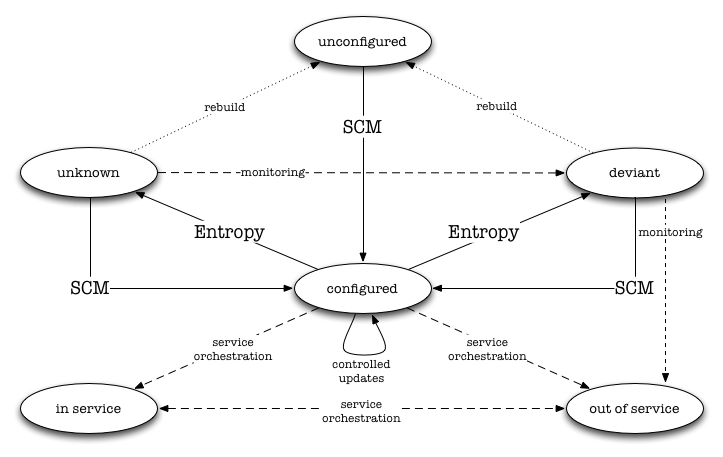
\includegraphics[width=0.95\textwidth]{07/pics/host-states}
		\caption[Host States in Configuration Management]{
			Different states a host may be in.  The CM tries to
			counter the effects of Entropy, while Service
			Orchestration controls e.g. whether a host takes
			traffic.  Monitoring of the systems may allow us
			to discover an ``unknown'' state or trigger a
			removal from service, while rebuilding a host
			allows us to ``start from scratch''.
			\label{fig:configuration-management:host-states}}
\end{figure}


\subsubsection*{Unconfigured}

A host in this state does not have a CM system
installed or the installed CM has never run.  The most
common example of hosts in this state is new hardware
that does not yet have an OS installed. Large
environments often have pools of new hardware
delivered, racked, and set up in their data center,
awaiting allocation.  Such systems are frequently in
this {\em unconfigured} state.

\subsubsection*{Configured} The CM has run
successfully and applied all required changes for the
given system.  All required packages are installed,
configured properly, and all services on the host are
running.  The system is ready for production.

\subsubsection*{In Service}  The host has been put
into production.  That is, it accepts traffic,
provides the service for which it was configured, and
is relied upon; it is in active use.  Technically
speaking, this is a subcategory of the ``configured''
state; a host may be put into service by other systems
than the CM -- we mentioned the concept of ``Service
Orchestration\index{Service Orchestration} -- but only
a ``configured'' host may enter this state.

\subsubsection*{Out of Service} The system has
explicitly been taken out of service; it is no longer
serving production traffic.  Unlike the remaining
states, this is a well-defined and known state.  The
CM is running and may even have placed the system into
this state as a reaction to a system or network
failure, possibly one outside of this host.  That is,
this state is also a subcategory of the ``configured''
state.  Once again, the host may be taken out of
service by another system than the CM.

\subsubsection*{Deviant}  The host is no longer in the
desired configuration state.  Entropy has taken its
toll: changes made to the system either manually or as
a side-effect of the traffic it takes, from individual
users or possibly even through a mistake in the CM
state model itself have caused a faulty configuration.
In this case, the configuration management system may
need to revert or otherwise correct these changes to
revert to the previous state.  Storing the rules for
the CM in a Version Control System makes such a ``roll
back'' easier.

\subsubsection*{Unknown} The CM may have stopped
running on the host or may erroneously be applying the
wrong configuration.  The host may have been shut
down, the network disconnected, an intruder may have
taken over control, or rats may have gnawed through
the power cable.  We simply don't know.  What's worse,
we may not even know that this host is in an unknown
state!  Not all failures are immediately obvious.  \\

Describing a service in detail, as we discussed
earlier in this chapter, and then applying the
required changes to a new host covers the steps to get
a system from the ``unconfigured'' state towards ``in
service''.  This involves a set of well-defined steps,
and the system remains in equally well-defined and
known states.

Much more challenging for both the CM as well as the
system administrators in charge are the prevention and
detection of the last two states, ``deviant'' and
``unknown''.  In order to recover and return the
system back to production, the software needs to be
able to identify error conditions and determine the
steps to correct them.  Automatic recovery from
certain failure scenarios is possible, and in fact
what we wish for our CM to provide.  However, most
software solutions can only handle previously defined
error scenarios; the nature of our systems inevitably
leads to unexpected failure modes.  Being able to {\em
detect} such deviant states is by itself a huge win,
as we can move from here into the much preferred ``out
of service'' state before resolving the root cause and
finally returning the host back into production.  In
some cases it may be easier and/or faster to reinstall
the host from scratch to bring it into a compliant
state.


\subsection{Sets}
\label{configuration-management:states-sets:sets}

Running any CM requires system administrators to
create and maintain a complex model of how services
are defined, what changes are required to enable or
disable a given component, and to keep track of all of
your systems in different environments with different
requirements.  The key to solving this puzzle is to
{\em simplify}: we take a step back and attempt to
identify the essential logical components of the
system.

In the previous section we have classified the
different {\em states} that our systems may be in, and
we have said that the role of a CM is the assertion of
a given state. But before we can express the changes
required to bring a host into a given state, we need
to have defined the role of each system.

%Enter Set theory.  Set theory is a wonderful thing.
%It allows us to completely abstract the functional
%requirements of configuration management into a
%well-understood model that is easy to follow.  Set
%theory allows us to group arbitrary resources and
%give each group a name.  With enough such carefully
%defined sets, we can describe a state model and apply
%it to our infrastructure.  Set theory resides at the
%core of configuration management. \\

Different CMs use different terms in their application
of several concepts that we borrow from Set Theory:
each solution allows for the grouping of certain
resources that can be combined using unions,
intersections, set differences, etc.  For example, sets of
changes or service definitions may be called
``manifests'', ``promises'', or ``recipes'', while
sets of hosts may be referred to as ``roles'', ``node
groups'', or they may be defined through the use of
``attributes'' or ``tags''.

I've found it useful to remember the visual
description of defining these sets as ``drawing
circles around things'': this is quite literally what
developers and system administrators often end up
doing on their whiteboards.  Looking at these
whiteboards or state diagrams immediately conjures the
Venn Diagram, an easy way for us to visualize
relationships between different groups.

As we define services as a set of changes, or hosts as
being grouped together by certain attributes, we can
build an inheritance model using further and further
abstraction of common properties into subsets.  By
performing set operations such as unions,
intersections and set differences, we gain significant
flexibility in determining common and service specific
definitions.

Let us take a look at the different kinds of resources we might draw
circles around:

\subsubsection*{Sets of changes}

Moving beyond maintenance of a few individual hosts,
we realize that changes made on our systems fall,
broadly speaking, into two categories: those that need
to be applied to {\em all} systems\footnote{Ok, we
are cheating a bit here: there rarely are properties
applying to absolutely {\em all} your systems.  In
System Administration in large scale environments,
exceptions are the single universal rule.} (as might
be the case illustrated by our \gls{ldap} Client
Configuration example from Section
\ref{configuration-management:defining-services:ldap-client}),
and those that need to be applied to only a {\em
subset} of systems, possibly a subset of one.  This
realization is fundamental: we begin to view system
configuration no longer as a task performed on an
individual host, but as {\em defining the changes}
that may need to be applied.

In addition, there are changes that are made to all
system {\em in exactly the same way} (e.g., the
{\tt /etc/sshd\_config} file is updated on all hosts to
disable {\tt PasswordAuthentication}) as well as
changes that are made taking specific properties of
the target environment into account (e.g. the use of a
different default route or DNS server depending on the
network the system is in).  The astute reader will
recognize parallels to the four classes of data we
identified earlier: ``static'', ``variable'',
``shareable'' and ``unshareable'' (compare Table
\ref{table:software-installation:shareable-variable}).

It is important to be consistent in the application of
this model:  even a single service running on a single
host should be well-defined and explicitly described
as such a set -- a set of one.  This allows us to
easily recreate the service in case of emergency, when
more resources are added, or when an additional
instance of the service is created, for example in a
new data center.

Figure
\ref{fig:configuration-management:change-states} shows
how different change sets can be combined via an
inheritance model to help define more complex
services.

\begin{figure}[!ht]
	\centering
	\includegraphics[width=0.80\textwidth]{07/pics/change-sets}
		\caption[Sets of changes applied to sets of hosts]{
			An illustration of how abstract
			change sets help define different services. Common
			modules are included in more complex definitions
			before being applied to groups of hosts.  Some
			``base'' modules (ssh and ldap in this example)
			are included on all hosts.
			\label{fig:configuration-management:change-states}}
\end{figure}

\subsubsection*{Sets of hosts}

Any host may, at any point in time, perform multiple
roles, offer multiple services, or meet multiple
requirements.  Grouping hosts according to their
properties, attributes, or functionality makes it
possible to apply the previously identified sets of
changes.  But groups of hosts are not only defined by
the services they provide; you can also categorize
hosts by different criteria even within a single
service definition.  It is common (and good practice)
to have for each service a small number of hosts --
some of which do not take any production traffic -- on
which to test any changes that we plan on rolling out.
Many organizations use the terms ``dev''
(development), ``qa'' (quality assurance),
``testing'', ``staging'' or ``canary'', and ``prod''
(production) for the different stages of software
development.  Likewise, it may be useful to group
hosts by geographical location to allow for a
carefully staged deployment on a global scale.

Software deployment -- an inherently risky business,
as we are willfully introducing entropy into a running
and stable system -- can thus be carefully
orchestrated through the use of a CM and clearly
defined roles.

In fact, CMs themselves usually allow you to {\em
branch} your changes in the same way that a software
development project may track different development
efforts before merging changes back into the main
line.  In order to take advantage of this approach,
divide your hosts into sets that are on a different
branch: a relativey small number of hosts would
receive all changes immediately, allowing the system
administrators to rapidly test all their changes; a
larger host sample (ideally including a cross section
of all possible host group definitions) should follow
the ``staging'' branch to which changes which need to
be tested would be deployed.  All remaining hosts
track the ``stable'' or ``production'' branch,
receiving changes only after they have gone through
the previous stages and found to be without errors.

See Section
\ref{configuration-management:fighting-entropy:deployment-roles}
for a more detailed description of this approach.

\subsubsection*{Sets of users}

Finally, account management is perhaps the most
obvious application of the principles of set theory
within configuration management.

As noted in Section \ref{multi-user:groups}, user
accounts may be grouped together by their required
access privileges.  Regardless of whether user
accounts are managed centrally via a directory service
or whether individual accounts are explicitly created
on each system, the decision to grant access is based
on a user's group membership ;  user groups are then
mapped to different sets of hosts as previously
illustrated in Figure
\ref{fig:multi-user:user-mappings}.

Note that different users can be simultaneously
members of multiple groups.  In our previous example,
we showed how users in the {\tt wheel} group were
given full {\tt sudo(1)} privileges on all hosts,
while members of the {\tt dev} group might only get
user level access to a small subset of all hosts.
These mappings are non-exclusive: a user may well be
in both the {\tt dev} and the {\tt wheel} groups at
the same time.


\section{Fighting entropy}
\label{configuration-management:fighting-entropy}

Configuration management asserts state.  That is, we
try to keep a system from deteriorating into an
undefined state and to (re-)establish more order.  We
continuously fight entropy.  But we are also
introducing change, and the changes we apply may have
side-effects.  CMs have the potential to completely
bring down an entire infrastructure if the wrong kinds
of changes are introduced.  It is therefore important
to look at a few safeguards and techniques that allow
us to prevent such disaster scenarios.

\subsection{Deployment roles}
\label{configuration-management:fighting-entropy:deployment-roles}

Managing infrastructure code, as it turns out, is not
very different from traditional software development.
The final product needs to be tested before it is
shipped to the customers.  In the context of
configuration management, this might be a service
definition that has to be verified to not
inadvertendly break the systems on which is should be
deployed, including new releases of the service
software.

As a result of this similarity, we usually employ
similar strategies and create development, test, and
pre-production environments on which to iterate
through a series of assertions to ensure the
correctness of the installation and configuration.  In
the previous section we already mentioned the grouping
of hosts into these conceptual roles -- and the number
of stages you require a change to propagate through
before it reaches production may depend on the size of
your environment -- but in general, it is a good idea
to have the configuration management development
process to include the following deployment roles.  As
you read through the description of these roles,
reference Figure
\ref{fig:configuration-management:host-sets} for an
illustration.

\begin{figure}[!t]
	\centering
	\includegraphics[width=0.65\textwidth]{07/pics/host-sets}
		\caption[Host Deployment Roles as Sets]{An illustration of
			the different deployment roles a host may be in.
			Of all hosts in the ``web server'' group, some are
			in the ``development'' environment, some are in the
			``test'' and ``staging'' environments, and some
			are serving production traffic.  Of those, a small
			subset performs the role of the ``canary''.
			\label{fig:configuration-management:host-sets}}
\end{figure}

\subsubsection*{Development}

These hosts serve as the playground where all
prototypes are initially set up as proofs of concept
before being properly packaged and turned into a
defined services.  All new changes are initially
developed and tested in this environment.  Hosts in
this role are often in a state of flux, and it is not
uncommon for a system administrator to break a service
in the process of testing a new configuration
management module.  For this reason, these systems do
not serve production traffic.

\subsubsection*{Test}

A small number of hosts on which to perform end-to-end
tests after initial development make up the test
environment.  Once we have defined a new service,
created a new package, or made any other changes to
our CM, we let them be applied in this environment.
The most important difference to the ``development''
environment is that {\em we do not perform any manual
changes here}: everything goes through the full
configuration management cycle.  This allows us to
make sure that the module we put together does in fact
include all required changes, can be applied by the
configuration management software, and does not cause
any obvious problems.

In a heterogenous environment it is import to ensure that all major
operating system versions are represented in this group.

\subsubsection*{Pre-Production}

Once testing has determined that the changes we plan
to roll out do indeed yield the desired state, we can
push them into the pre-production environment,
sometimes referred to as ``staging''.  This group
consists of a representative sample of all production
serving hosts, including different hardware
configurations and different operating systems.  For
each major service, a sample of hosts are placed into
this role to ensure compatibility of any new changes
within the given software stack.

Systems in this role do not usually take full
production traffic, but may be used internally to test
your products.  In some environments, a small
percentage of actual production traffic is shifted to
these systems to ensure that all crucial code paths
that might be encountered once the change is deployed
are executed.

Often times we define automated checks and tests that
run against these hosts to ensure no unexpected side
effects were introduced by the changes we made.

\subsubsection*{Production} All hosts serving
production traffic or providing a crucial (possibly
internal only) service.  Any changes made here should
have gone through the previous stages, and in some
cases may require explicit ``change
management\index{change management}'' practices,
including advance notification of all stakeholders,
service owners, and customers.

Since this group of systems can range in size from
only a handful of hosts (for a particular service) to
literally hundreds of thousands of machines (providing
multiple services), deployment of any changes is
inherently risky and needs to be coordinated
carefully.  Especially in very large environments
these changes are often deployed in a staged manner:
starting with a small number of machines the
percentage of all hosts that will receive the change
is slowly ramped up.

\subsubsection*{Canary} Sometimes it is difficult to
account for all eventualities, and experience has
shown that some errors cannot (easily) be reproduced
or triggered in a controlled staging environment.
This is largely due to the fact that actual production
traffic is so difficult to simulate.  Hence, it may be
a good idea to create a so-called ``canary'' role as a
special method of detecting possible errors in your
configuration:  individual hosts that are part of the
actual production environment and that do take
production traffic will get code deployments earlier
than the bulk of the production hosts.  This way,
errors can be detected before they might be deployed
everywhere else.  Like the canary in the coal mine,
these hosts serve as an early warning system for
potentially dangerous changes.

\begin{sidenote}
{\bf Security Roles} \\

Please note that the definitions given here are also
helpful in deciding access control as well as traffic
flow from a security perspective.  For example, hosts
in a {\em development} role may be accessed by all
developers, while production systems may not.
Similarly, traffic may be allowed from hosts in the
``test'' role to other hosts in the same role only,
but access of production data may be restricted to
production systems only. \\ [10pt]

Even though there is a certain overlap in defining
deployment roles and in defining roles related to
security, they are not always congruent.  While access
restrictions may be derived from the deployment model,
finer grained control and additional restrictions or
definitions are often necessary.  Nevertheless, the
model of {\em sets} applies here as well.  Only this
time, we are, for example, drawing circles around
host- and network based \gls{acl}\index{Access Control
Lists} and intersecting these security roles with
host- and user groups.

\end{sidenote}


\subsection{Idempotence and Convergence}
\label{configuration-management:fighting-entropy:idempotence-convergence}
\index{Idempotence}
\index{Convergence}

Configuration management asserts state.  To this end,
it must reliably produce a defined state without
side-effects and needs to be able to run under
different circumstances, yet yield the same outcome.
If you run your CM on an unconfigured system, it will
produce the same end-result as if you run it
repeatedly, over and over, in its final, configured
state.

Operations that can be performed multiple times yet
always produce the same result are called {\em
idempotent}.  To illustrate, unary mathematical
operations are idempotent if the following definition
holds:

\begin{displaymath}
f(f(x)) \equiv f(x)
\end{displaymath}

That is, a function applied twice to any value will
produce the same result as if applied only once.  A
common example here is taking the absolute value of
$x$:

\begin{displaymath}
| |-1| | \equiv |-1|
\end{displaymath}

%For binary operations, the definitions get a bit more
%complicated: an idempotent function applied to two
%equal values will return that value (e.g. $max(x,x)
%\equiv x$), but for other operations there may exist
%only some elements that satisfy idempotence:
%multiplication by $0$ or $1$, or division by $1$, are
%examples of idempotent elements on binary operations:
%no matter how often you repeat this operation, the
%end result will remain identical.

How does this property translate into practical
applications within the scope of configuration
management?  As we are moving the system from one
state to another, we are applying certain changes.
Executing these steps must not yield different results
depending on the previous system state.  Reviewing the
required capabilities we identified as CM requirements
in Section
\ref{configuration-management:defining-services:requirements}
-- software installation, service management, file
permissions and ownerships, installation of static
files, generation of host-specific data, and command
execution -- we find that each may or may not be
implemented in a manner that satisfies this
requirement.  As one example, assertion of an existing
file's ownership and permissions, is an inherently
idempotent operation: no matter how often you execute
these commands, and no matter what the permissions and
ownership on the file were before, the end result will
be the same.

Other typical tasks within configuration management
are not quite as obviously idempotent, and some --
updating an existing file on a host with parameters
determined at runtime, for example -- may in fact
not be.  For any command executed within a
configuration management system, you can ask yourself
the question of whether or not the outcome will be the
same if you either run the command under different
circumstances, or if you repeat the command over and
over.  See Listing \ref{code:cm:idempotence} for a few
trivial examples.  Note that sometimes a command may
behave idempotently only if a special flag is given, and
that under some circumstances the only thing that
makes a command {\em not} idempotent may be the exit
status.  (We will revisit the importance of
idempotence within the context of building scalable
tools again in Chapter
\ref{chap:building-scalable-tools}.)

\begin{lstlisting}[basicstyle=\scriptsize,float,label=code:cm:idempotence,caption={Idempotent and non-idempotent commands.}]
$ cd etc                                            # not idempotent
$ rm resolv.conf                                    # idempotent
$ echo "nameserver 192.168.0.1" > resolv.conf       # idempotent
$ echo "nameserver 192.168.0.2" >> resolv.conf      # not idempotent
$ chown root:wheel resolv.conf                      # idempotent
$ chmod 0644 resolv.conf                            # idempotent
\end{lstlisting}

In many cases the CM may aid in defining actions in
such a manner as to preserve idempotence -- {\em
CFEngine}, for example, explicitly discourages the use
of free shell commands and leads the user to abstract
their requirements into so-called
``promises''\cite{configuration-management:cfengine-manual}
-- but in the end it is up to the system administrator
to carefully evaluate the service definitions and
change sets she creates and applies to ensure that no
side-effects are possible.

Idempotence goes hand in hand with the philosophy of
asserting state, rather than making changes.  Writing
system tools and defining changes that are idempotent
takes great care and consideration, especially when
one considers the possibility of simultaneous
execution of commands or programs outside of our
control.  The time and effort spent on identifying
these and creating a tool that can cope with these
factors yield significant benefits: System stability
increases as we are able to reliably repeat the same
commands without fear or unwanted side-effects.  \\

It is important to note that idempotence does {\em
not} imply that an operation is {\em only} performed
when it is necessary, only that the {\em outcome} will
remain the same.  That is, idempotence does not
guarantee efficiency nor necessarily continuous
service availability.  Consider two systems, one brand
new and unconfigured, one already in a desired state,
i.e. a production service.  In order to get the first
system into the state of the second system, the CM
needs to make a lot of rather intrusive changes:
software packages have to be installed, configuration
files updated, and the host may need to be rebooted,
possibly multiple times.  Performing all of these
steps again when the end state would be the same as
the current state seems like a bad idea.  At best,
we'd be wasting CPU cycles; at worst, we'd introduce
temporary instability or service downtime.

This is where the concept of {\em
convergence}\index{Convergence} comes into play:  A
configuration management system should only perform
those operations and apply only those changes that are
necessary.  Idempotence and Convergence are easily
conflated, and within a CM, both are desired
properties.  But it is important to be aware of the
difference:

Consider the \verb+chown(8)+ and \verb+chmod(1)+
example code from Listing \ref{code:cm:idempotence}.
Despite being idempotent, running the commands may not
be necessary at all if the permissions and ownerships
are already as desired.  That is, the configuration
management system could first test for the desired
end-state, and then only execute the steps missing.
In this particular example, the difference is
negligible, but the practice of checking whether
commands actually need to be executed becomes more
important when we consider how our system may assert
the presence of a certain software package.

That is, if a package of the required version is
already installed, the CM (possibly by way of the
package manager it invokes) will likely perform a
no-op instead of fetching the same package and
re-installing it.  This is {\em not} the same as
performing the installation again:  for example, all
too frequently poorly packaged software may overwrite
your carefully tuned existing configuration file with
a new template or example file.  A good package
manager, and a carefully written package, may be able
to prevent this from happening, but you cannot always
rely on this.

Different CMs provide different features, and being
able to use them all to your advantage requires
practice.  In some systems, the responsibility of
defining convergent operations is pushed on the system
administrator; other CMs go to great lengths to avoid
unnecessary changes.  Idempotence is crucial for all
operations within a CM, but allowing the system to
reach the end state in a convergent manner improves
stability and reduces the possibility for service
interruptions on the way from state A to state B.
Both principles are often fully understood and
appreciated only after a lot of practical experience
and a perhaps a few ``interesting'' error scenarios,
but try to keep them in mind as you develop and deploy
your CM solution.

\subsection{Quis custodiet ipsos custodes?}
\label{configuration-management:quis-custodiet}

The latin phrase ``{\em Quis custodiet ipsos
custodes?}'' -- translated: ``Who will guard the
guards themselves?'' -- expresses a fundamental
dilemma we encounter when we give full control to any
person, government body or, in our case, a piece of
software.  That is, configuration management asserts
state, but what ensures that the configuration
management system functions properly?

In fact, CM systems usually control {\em themselves}.
After all, configuration management is a software
service just like any other, and needs to be
controlled and monitored the same way.  This, however,
introduces a rather significant risk factor, as
changes made to the CM itself have the ability to
either wreak havoc across the entire infrastructure or
to simply halt any progress if it breaks down.

For this reason, it is important to put in place
safeguards and practices to reduce the probability of
such errors.  The risk of potential disaster is one of
the side effects of a high degree of automation.  We
will discuss this and a number of possible risk
mitigating techniques in detail in Chapter
\ref{chap:automation}.

\section{Even more formal process definitions}
\label{configuration-management:formal}

Today's CM systems exhibit a noticable overlap with
concepts discussed in the \gls{itil}\index{Information
Technology Infrastructure
Library}\cite{configuration-management:itil}, a set of
practices underlying the first international standard
for IT Service Management, ISO/IEC 20000\index{ISO/IEC
20000}.  As a formalized standard trying to cover
generally applicable practices, these documents offer
a far from thrilling reading experience and have seen
limited voluntary adoption in the private sector.  The
main criticisms are similar to those applied to
similar standard documents and regulations (such as
the notorious \gls{pcidss}\index{PCI DSS}): good
intentions and sound general advice is lost amidst
lenghty rationale and overly bureaucratic and much too
broad definitions.

As perhaps a form of social commentary, one might be
further inclined to seek parallels between modern CM
systems and a general Silicon Valley startup culture
of rapid invention and quick iteration versus an as
``old and stuffy'' dismissed IT process represented by
the formality of \gls{itil}.  As so often, software
systems reflect the organizational and cultural
hierarchies under which they are
developed\footnote{See ``Conway's Law'', derived from
\cite{configuration-management:conways-law}\index[names]{Conway,
Melvin E.}.}; most System Administrators with
sufficient experience will find some humor in the fact
that nevertheless, even these different methodologies
become eventually convergent.

That is, despite being easily dismissed as not
flexible enough for practical application, many of the
recommendations or best practices outlined in ITIL do
underly or correlate to the operations of modern CMs.
For example, large scale configuration management has
evolved to effectively implement or require a
repository of all information about the various
systems in an organization, the Configuration
Management Database\index{Configuration Management
Database} (or CMDB).  When you read up on this topic,
you will hopefully be able to relate those documents
to a number of concepts discussed here.




\section{Summary}
\label{configuration-management:summary}

We have covered a lot of ground in this chapter, much
of it theoretical.  The examples shown were taken from
some of the more popular configuration management solutions
currently in use: CFEngine, Chef, and Puppet.  All
three implement their own Domain Specific Language,
with striking similarities amongst them.

We identified as one crucial concept in configuration
management the idea that services are abstracted from
the hosts that provide them.  This abstraction allows
us to define not individual changes, but rather
self-contained change sets describing what is required
to provide a given functionality.  These change sets,
in turn, can be applied to groups of hosts; with those
sufficiently abstracted and clearly defined, we are
able to combine attributes of host groups and describe
its members' final state using set operations.  Much
like on a white board or the proverbial paper napkin
in a restaurant, we draw circles around things.
Giving those circles descriptive names, configuration
management then becomes a question of creating unions
or intersections of service descriptions with host
collections.

Using this model, we determined that configuration
management is really not about {\em applying changes},
but about {\em asserting state}, ensuring that a host
meets a certain set of criteria.  We have looked at
the functional requirements any CM needs to provide in
order to yield a desired state as well as the
essential concepts of idempotence and convergence: all
changes we make must have well-defined and predictable
outcomes that do not change if applied repeatedly; at
the same time, we only want to perform those changes
that are necessary.

When building our infrastructure we face a choice
between a custom, home-grown system that integrates
perfectly with other system components, and deploying
an ``Off The Shelf'' solution.  Many commercial
products exist that promise to manage all of your
systems with ease.  Some of them offer free versions;
some systems are available as open source software,
while others are closed.

Knowing our infrastructure needs inside and out, we
often fall into the trap of writing our own solutions.
In small environments, the benefits of a complex
product do not seem worth the cost of adapting our
infrastructure to abide by the product's configuration
model.  It is for this reason that every growing
company inevitably undergoes a phase during which
large parts of the initial infrastructure are ripped
out and replaced by more scalable solutions --
including a mature configuration management system.

In very large environments, on the other hand, our
requirements are so unique as to not likely to be
matched trivially by any available solution; we will
need to write a significant amount of ``glue'' code
around the product anyway -- why not just implement
our own system?  But therein lies a frequent fallacy:
as any software engineer knows, the best code is the
one we do not have to write ourselves.

Fortunately, development on a number of flexible CMs
has yielded several viable solutions for almost any
scale.  A small environment benefits from the rigorous
structure imposed by a mature configuration management
system able to grow with the infrastructure; in large
environments, it is useful to be able to rely on a
proven technology and focus on the end point
integration with other systems.  \\

The area of configuration management has become one of
the most important fields in large scale system
administration and has opened up room for a lot of
interesting research.  As this chapter hints at, there is
significant overlap between configuration management,
software provisioning\index{Provisioning}, and the
many related tasks in ensuring reliable service
availability.  All of these moving parts are sometimes
referred to as ``Service Orchestration''\index{Service
Orchestration}, by now its own field of research
covering the theory of how complex systems fail, in
how far we can achieve automatic recovery or guarantee
service availability, and the concept of autonomous
state configuration across large scale deployments
with literally hundreds of thousands of hosts.  See
Figure \ref{fig:configuration-management:cm-overlap}
for an illustration of these relationships.

\begin{figure}[!t]
	\centering
	\includegraphics[width=0.65\textwidth]{07/pics/config-management-overlap}
		\caption[Configuration Management Overlap with other systems]{
			Configuration Management overlaps and
			intersects several other areas
			of System Administration, many
			of which depend on a central asset database and
			comprehensive service definitions.
			\label{fig:configuration-management:cm-overlap}}
\end{figure}

As so often, we can only focus on the fundamental
concepts with just enough references to more advanced
topics to entice the reader to continue their
research. We will revisit some of these topics in
section \ref{sec:missing:service-orchestration}, when
we try to catch up on missed topics and tie together
some of our loose ends. \\

Throughout this chapter, we have focused primarily on
configuration management of host-type systems.  But
our infrastructure consists of more than just
``hosts'': we have large amounts of network
equipment as well as a number of appliances that sit
somewhere in between the traditional networking gear
and a ``normal'' host: we have routers and switches,
load balancers and firewalls, storage devices and
intrusion detection systems... the list goes on.  All
of these devices {\em also} require configuration
management, and it is unfortunate that integrating
them into your existing CM is often difficult, if not
impossible.

Our approach to divide resources into grouped sets and
describe changes as service definitions does in fact
translate to non-host systems as well.  All we need is
for a programmatic method to access them -- ideally,
though not necessarily via a programmable interface
such as a well-documented \gls{api} -- and we can add
support for them to our CM.  A positive development in
recent years has lead some of the configuration
management tools we mentioned to now allow you to
manage at least some non-host type systems, even
though we are still a ways from the same level of
control.  \\

The fundamental value configuration management provides as
we move from individual systems to easily replicated
services is perhaps best summarized by this quote:

\begin{quote}
``The test we use when designing infrastructures is "Can I grab a random
machine that's never been backed up and throw it out the tenth-floor
window without losing sysadmin work?" If the answer to this was "yes",
then we knew we were doing things
right.''\cite{configuration-management:traugott}
\end{quote}

Granted, one would hope that people entering your
datacenter and throwing machines out of the window is
not a regular event.  But Murphy's famous
law\index{Murphy's Law} -- commonly cited as ``Anything
that can go wrong, will go wrong.'' -- acts as
viciously, and we must view software failure as the
functional equivalent.  All software has bugs, and it
is only a question of time until your complex service
encounters a fatal error.  Similarly, hardware fails
as well -- and not too infrequently.  This becomes
painfully obvious in very large environments with
hundreds of thousands of machines, as the probability
of encountering a hardware failure increases
proportionally to the number of hosts in service.
``One in a million is next
Tuesday.''\cite{configuration-management:next-tuesday}

With properly defined services, correctly grouped
hosts, and a well running CM individual hosts do
become expendable.  Any system-, software-, or
hardware failure has significantly reduced impact on
our overall service availability.  In other words:
configuration management lies at the heart of any
well-managed infrastructure and makes large scale
deployments ultimately maintainable.

\vfill
\pagebreak

\chapter*{Problems and Exercises}
\addcontentsline{toc}{chapter}{Problems and Exercises}
\section*{Problems}
\addcontentsline{toc}{section}{Problems}

\begin{enumerate}

\item

Review your own environment, your infrastructure, and
your essential services.  Do you think they could be
rebuilt from scratch?  With how much effort?  Which
components seem completely and easily replaceable, and
which would you fear most to lose?

\item

Identify the configuration management system currently
in use on the systems you have access to.  Can you
determine which components or services are controlled
by the CM in question and which resources are not?
Contact your system administrator and ask her about
details.

\item

Review the documentation for one of the popular CMs.
Most of them can quickly and easily be tried out using
just a few virtual machines.  Set up a CM and try to
define a simple service.  How does this system
implement the features and concepts we discussed?

\item

Pick a popular service provided in your environment --
for example a DNS-, web- or file server -- and create
a complete service definition for it.  Make sure to
identify the smaller required modules this service
relies on.  How far does it make sense to abstract the
individual components?

\item

When deploying a new service, identify the different
categories into which each step falls.  Is software
installation sufficiently covered by executing the
right commands using your package manager?  Do
additional files need to be created or existing
configuration files modified?  Does the configuration
file differ from host to host within a service group?

\item

Review how your existing package management system
handles reinstallation of a package of either the same
or a different version.  How are configuration files
handled?  Are these actions idempotent?

\item

Consider the agent bundle shown in Listing
\ref{code:cm:cfengine:dynamic-restart}.  What kind of
parameters in the {\tt sshd\_config} file would you
expect to be expanded when this code is executed?
Using CFEngine's online documentation, create a
suitable template.

\item
Review the commands shown in Listing
\ref{code:cm:idempotence}.  Do you agree with their
classification as being idempotent or not?  Try to
argue for or against their classification.

\item
Consider the command ``{\tt mv this there}'' -- under
what circumstances is this particular invocation
idempotent?  Is it ever?  What, if any, checks or
changes can you add to a script that includes this
command to ensure the outcome {\em is} idempotent?

\item
A common test of a new CM consists of updating the
{\tt /etc/motd} file with information from the running
host.  This operation incurs a very small risk, as no
application relies on this file, yet it can easily
show that the system is running and operating
properly.

Create a script or command to update the {\tt
/etc/motd} file on a system to include the hostname of
the system, the time since the host was last rebooted,
and the time this script was last executed.  Can you
translate this script into a template in the \gls{dsl}
of your configuration management system?

\item
Review the different states your systems may go
through.  How do you currently define a properly
operating host?  How would you go about identifying a
{\em deviant} host?

\item
Every System Administrator has a virtual tool chest
full of scripts, commands, and utilities used during
the configuration and maintenance of their systems.
Review your peers' tools as well as your own and
identify in how far they assure {\em idempotence} or
{\em convergence}.  Compare these to the common tools
provided by your Unix systems (such as the scripts
found under {\tt /etc/rc.d} or {\tt /etc/init.d}) or
shipped with a given software package.

\end{enumerate}

\vfill
\pagebreak

\bibliographystyle{plainnat}
\begin{thebibliography}{99}

\bibitem{configuration-management:burgess:cfengine} Mark Burgess, {\em A
Site Configuration Engine}, USENIX Computing systems, Vol8, No. 3, 1995;
on the Internet at 
{\url http://cfengine.com/markburgess/papers/paper1.pdf} (visited February
22, 2013)

\bibitem{configuration-management:nelson-smith:chef} ``An Overview of
Chef'', on the Internet at
{\url http://docs.opscode.com/chef\_overview.html} (visited February 23,
2013)

\bibitem{configuration-management:turnbull:pro-puppet} James Turnbull,
Jeffrey McCune, {\em Pro Puppet}, Apress, 2011

\bibitem{configuration-management:ansible} ``Ansible
Documentation'', on the Internet at
{\url https://docs.ansible.com/} (visited March 18,
2017)

\bibitem{configuration-management:itil} Cabinet Office, {\em ITIL
Service Operation 2011 Edition (Best Management Practices)}, The
Stationery Office, 2011

\bibitem{configuration-management:burgess:immunology} Mark Burgess, {\em
Computer Immunology}, Proceedings of the Twelfth Systems Administration
Conference (LISA 100) Boston, Massachusetts, December 6-11, 1998,
USENIX Association, Berkeley, CA, 1998; on the Internet at
{\url
http://www.usenix.org/event/lisa98/full\_papers/burgess/burgess.pdf}
(visited January 29, 2013)

%\bibitem{configuration-management:set-theory} Georg Cantor, ``\"{U}ber eine
%Eigenschaft des Inbegriffs aller reellen algebraischen Zahlen'', Journal
%f\"{u}r die reine und angewandte Mathematik, 1874; on the Internet at \\
%{\url http://www.digizeitschriften.de/main/dms/img/?PPN=GDZPPN002155583}
%(visited March 10, 2013)

\bibitem{configuration-management:turing-equivalence} Steve Traugott,
Lance Brown, {\em Why Order Matters: Turing Equivalence in Automated
Systems Administration}, Proceedings of the USENIX Large Installation
System Administration conference, Philadelphia, PA Nov 3-8, 2002,
USENIX Association, Berkeley, CA, 2002; on the Internet at
{\url http://www.infrastructures.org/papers/turing/turing.html} (visited
January 29, 2013)

\bibitem{configuration-management:burgess:models-myths} Mark Burgess, {\em
Configuration Management, Models and Myths},  Originally published in
Usenix ;login: 2006-2007; on the Internet at
{\url http://cfengine.com/markburgess/cm.html} (visited January 29, 2013)

\bibitem{configuration-management:brooks-design}Frederick P. Brooks, Jr.,
{\em The Design of Design}, Addison-Wesley Professional, 2010

\bibitem{configuration-management:cfengine-manual} {\em CFEngine
Documentation}, on the Internet at
{\url https://cfengine.com/manuals/}

\bibitem{configuration-management:burgess:rosegarden} Mark Burgess, {\em
Promise you a Rose Garden}, On the Internet at
{\url http://cfengine.com/markburgess/rosegarden.pdf} (visited January 29, 2013)

\bibitem{configuration-management:lueninghoner} Cory Lueninghoner, {\em
Getting Started with Configuration Management}, Originally published in
Usenix ;login: April 2011, Volume 36, Number 2; on the Internet at
{\url https://www.usenix.org/system/files/login/articles/105457-Lueninghoener.pdf}
(visited January 29, 2013)

\bibitem{configuration-management:burgess:testable} Mark Burgess, {\em
Testable System Administration}, in {\em ACM Queue}, January 2011, Vol. 9
No. 1, ACM, New York, NY; on the Internet at
{\url https://queue.acm.org/detail.cfm?id=1937179} (visited January 29, 2013)

\bibitem{configuration:management:couch} Alva Couch, Yzihan Sun, {\em On
the Algebraic Structure of Convergence}, in {\em Proc. 14th IFIP/IEEE
International Workshop on Distributed Systems: Operations and Management},
Heidelberg, Germany, Springer-Verlag, Inc, pp. 28-40

\bibitem{configuration-management:traugott} Steve Traugott, Joel
Huddleston, Joyce Cao Traugott, {\em Best Practices in Automated System
Administration and Infrastructure Architecture: Disaster Recovery}; on the
Internet at
{\url http://www.infrastructures.org/bootstrap/recovery.shtml} (visited March
09, 2013)

\bibitem{configuration-management:conways-law} Melvin
E. Conway, {\em How Do Committees Invent?}, in {\em
Datamation magazine}, April, 1968; on the Internet at
{\url
http://www.melconway.com/Home/pdf/committees.pdf}
(visited April 04, 2017)

\bibitem{configuration-management:next-tuesday} Larry
Osterman, {\em One in a million is next Tuesday},
March 30, 2004; on the Internet at
{\url
http://blogs.msdn.com/b/larryosterman/archive/2004/03/30/104165.aspx} (visited April 04, 2017)

\end{thebibliography}

\chapter{Automation}
\label{chap:automation}

\begin{figure}[h]
\begin{tabular}{l r}
\hspace{-1cm}\begin{minipage}{.85\textwidth}
\begin{quote}
{\em The first rule of any technology used in a
business is that automation applied to an efficient
operation will magnify the efficiency.  The second is
that automation applied to an inefficient operation
will magnify the inefficiency.}
-- Bill Gates\index[names]{Gates, Bill}
\end{quote}
\end{minipage}
&

\raisebox{-.8\height}{
	\includegraphics[width=.25\textwidth]{08/pics/wall-e} }

\end{tabular}

\label{fig:wall-e}
\end{figure}

\section{Introduction}
\label{automation:introduction}

In the previous chapter we have discussed how
configuration management systems allow us to create
abstract service definitions and apply the required
changes on the desired sets of hosts.  CM systems thus
remove the need for manual configuration on individual
hosts -- we have automated the steps, and in the
process improved the reliability and scalability of
our services within the infrastructure.

Similarly, we have hinted in Section
\ref{software-installation:os-installation} at systems
capable of performing OS installations across large
numbers of hosts without human intervention.  Knowing
all the individual steps needed to install an
operating system, adding the required software, and
performing initial host configuration (before we
finally let our configuration management engine take
control) allows us to use software to repeat a
previously tedious manual procedure hundreds of times
a day with great ease.

Both of these admittedly complex systems are prime
examples of what system administrators do best: being
inherently ``lazy'' -- a virtue, as we will discuss a
bit more in a minute -- we automate any conceivable
task such that it can be performed at the push of a
button, or perhaps more likely, the press of the
$return$ key.

In this chapter, we will take a small step back
from these large infrastructure components and review
the motivation of the more general concept of
``automation''.  Given the incredible variety of job
descriptions and environments a system administrator
might find herself in, it is not surprising that
the idea of letting computers do our bidding has found
a number of different practical approaches.  We see
evidence of automation as much in a system
administrator's shell aliases or custom scripts as in
the regularly scheduled {\tt cron(8)}\index{\tt
cron(8)} jobs or manually invoked tools.

It has been an old joke that the goal of any great
system administrator is to automate themselves out of
a job, just as we like to suggest to our colleagues or
peers that they should stop bothering us, lest we
replace them with a small shell script.  The use of
this language reflects how we approach automation: our
goal is to not have to perform certain tasks
ourselves, and anything that can be automated, will
be.

Unlike humans, computers do not seem to mind
performing boring, repetitive tasks.  This chapter
looks at how we can take advantage of this fact, how
automation can help you stop wasting your time, and
put to greater use the most valuable resources in any
organization (your engineers' minds). But automation
is no panacea, so we necessarily identify a number of
possible pitfalls and risks as well.

\section{Of Laziness And Other Virtues}
\label{automation:laziness}
\index{Laziness}

System administrators are notoriously lazy.  We don't
want to have to manually swap backup tapes every other
day -- we'd much rather let a robot perform this task.
We don't want to download, extract, build, and install
software packages, hunting down dependencies in the
process -- we'd much rather let our package manager
take care of this.  And we certainly do not want to
sit there all day typing the same set of commands over
and over, when we could instead apply our, in our
humble opinion, significant intellect to solving
mankind's greatest mysteries, such as why the label
maker always runs out of tape in the middle of cabling
a new rack.\footnote{We could, of course, write a quick
script that periodically checks the inventory system
and orders new label maker tape online whenever the
stock supply of label maker tape drops below a given
threshold...}

But being lazy is a virtue -- in this case, anyway.
In order to develop a solution that will save us
tedious work in the long run, we are willing to invest
significant resources up front.  We write scripts that
will take into account a variety of circumstances in
order to allow us to run just one command instead of a
dozen, we schedule checks and implement monitoring
solutions to be notified of events before they become
error conditions, and we write tools that react to
these alerts and which will automatically avert
impending doom.

\AE leen Frisch identified\cite{automation:frisch} --
only slightly tongue-in-cheek -- a number of
``administrative virtues'': Flexibility, Ingenuity,
Attention to Detail, Adherence to Routine,
Persistence, Patience, and Laziness.  While these
traits come into play in almost any of a system
administrator's varied duties, there are particularly
strong parallels to the features that allow us to
create reliable automation tools:

We need {\em flexibility} and {\em ingenuity} to
identify new and perhaps not entirely obvious
solutions to the problems we encounter.

We need to pay {\em attention to detail}, to the
nuances in the ways our systems may differ, when we
analyze and identify all the possible edge cases, or
how invoking a command under certain circumstances can
lead to unexpected results.

We need a strict {\em adherence to routine} to produce
reliable results, to collect usable data, and to keep
our systems maintainable.  We need to follow our own
processes even when we are under pressure and inclined
to take shortcuts, because we trust the routine we
identified earlier more than we trust our stressed out
brains.

We need {\em persistence} and {\em patience} when we write
software, when we debug our tools, when we collect
enough data to be able to identify our outliers and
averages, and we need persistence and patience when we
deploy our new systems, our infrastructure components,
or when we slowly, carefully, replace a much needed
service with different software.

But what impacts most of our practical work turns out
to be {\em laziness}.  As soon as we run a lengthy command a
second or third time, or as we repeat a series of
complex steps to complete a specific task, we start to
wonder how we can script this.  Sure, we may end up
spending a lot of time getting our automated jobs just
right, but we gain productivity in the long run.  And
so our laziness pays off.

\section{Benefits of Automation}
\label{automation:benefits}

When we look at large infrastructure components that
help automate a complex process or workflow such as
the deployment of a new host, it is immediately
obvious that we reap significant benefits from having
developed such a system.  But even on a much smaller
scale do we discover the same advantages, even though
we may initially begin the process of automating a
given task with the only goal being to save ourselves
some typing.  The primary benefits we derive from
implementing an automated solution -- even in the
small -- include the following.

\subsection{Repeatability}
\label{automation:benefits:repeatability}

Typing the same set of commands over and over is
tedious.  A few years ago, while maintaining a
heterogenous environment of NetBSD/i386 and IRIX/mips
systems, I had to try to keep in sync the latest
version of the \gls{gcc}\index{\tt gcc(1)},
standardizing it to fit into our environment, enabling
only the required languages but at the same time
ensuring the build of a 64-bit binary\footnote{Certain
64-bit capable IRIX systems supported both a 32-bit
and a 64-bit \gls{abi}\index{Application Binary
Interface}; in order to use the more performant 64-bit
interface, the application would have to be compiled
with support for and be linked against the 64-bit
libraries.  Even though less common today, you can
still find a number of tools that cannot (easily) be
built as 64-bit binaries.}.

Normally, you would have your package manager perform
this installation.  However, as discussed in Section
\ref{software-installation:package-management:manual},
there are situations where installing software ``by
hand'' is your only option.  This was one of them: the
native package manager did not provide a 64-bit
version of this compiler, and what might otherwise
seem like a routine task -- building a new compiler --
required the setting of a number of environment
variables and command-line options to the {\tt
./configure} script.  In order not to have to remember
all the right settings, I wrote myself a trivial
script (see Listing \ref{code:automation:gcc}.

\begin{lstlisting}[float,label=code:automation:gcc,caption={[Script
to build GCC on an old IRIX system]Building a 64-bit
version of the GNU Compiler Collection on an old IRIX
system. Even if done rarely, storing these commands in
a rudimentary script can help repeat the process more
easily. (With plenty of room for improvement, Problem
\ref{prob:automation:improve-script} will ask you to
turn this into a more reliable, more readable tool.)}]
#! /bin/sh
export CC=cc CXX=CC CFLAGS="-64 -mips4 -r10000" LDFLAGS="-64"
mkdir gcc-build
cd gcc-build
../gcc-3.3.3/configure --prefix=/usr/pkg/gcc-3.3.3         \
        --enable-languages=c,c++,java --enable-libgcj      \
        --disable-shared --enable-threads=posix            \
        --enable-version-specific-runtime-libs             \
        --enable-haifa --disable-c-mbchar                  \
        --disable-checking --disable-nls
gmake bootstrap
\end{lstlisting}

A few months later, when a new version of
\verb+gcc(1)+ became available, I had to repeat the
same process.  Instead of wasting time trying to
remember all the options I needed, what environment
variables I had to set, etc., I was able to build it
using this trivial script.

We often use automation as a way to remember the
correct steps.  Even a task that is not performed
frequently -- in our example above, perhaps twice a
year -- benefits from us creating even a simple script
to repeat it easily without having to think twice
about every detail.  Detailed documentation explaining
{\em why} certain parameters need to be passed may be
ideal, but providing a simple script to repeat a
cumbersome process is still a win.

Guaranteed repeatability allows us to ignore {\em how}
a task is performed.  Even simple scripts can thus
hide unnecessary complexity from us, making the task
at hand easier in the process.

\subsection{Reliability}
\label{automation:benefits:reliability}

Being able to repeat the same process easily without
having to recall the details of every step is a great
advantage, not only because it saves us a lot of
typing or because we don't waste time recreating
previously known information.  One of the key benefits
of an easily repeatable process lies in its {\em
reliability}.  When we run commands interactively, we
may change the order or detail of invocation as we run
through the end-to-end process.  We easily make
mistakes, mistype a command, accidentally redirect
output to truncate a file instead of appending to it,
accidentally slip in an additional character, execute
a command from the wrong directory, or we simply skip
a step (by accident or because we deem it
unnecessary).

Every time we invoke a script, on the other hand, it
will run the same commands in the same order.  If we
are careful when we automate a task and create a tool
executing idempotent commands only (hopefully combined
with copious error checking), we need not worry about
how it is invoked.  We can treat it like any other
system utility and rely on it running either to
completion or produce meaningful error messages that
allow us to diagnose the problem.

Automation provides reliability not only through
consistency, but also in terms of quality: as soon as
we begin to automate a task, we begin to move beyond
just stashing individual commands in a script (such as
the one given as an example above).  Instead, we build
our tool with reliability in mind, fine tuning the
steps and beginning to think more about how they are
executed.  Just like documentation, we are more likely
to consider in more detail the implications of each
command when we create an automated job.  As a result,
the final utility is more robust and executes more
reliably than any manual process ever would.

Some tasks need to be performed repeatedly with a
certain regularity, system backups being a prime example.
For starters, the backup process needs to be
run on a daily basis.  Defining the command required
to initiate this task and then scheduling it via the
{\tt cron(8)} d\ae mon is about as mundane yet
important a task as you may encounter in any system
administrator's life.  But being able to rely on the
tool is a pre-requisite, and automating the steps to
allow them to be scheduled in the first place does
provide this required reliability.

\begin{experience}
{\bf Robots to the rescue!} \\

Automation can not only be achieved by scripting or
programming.  Several years ago, it was not uncommon
for small sites to use a single tape
library\index{tape library}, storing backups on a
rotating set of backup tapes.  This meant having to
change the tape on a daily basis, as otherwise you
would overwrite the previous day's backup.  It turns
out that most humans are fairly bad at remembering
such tasks -- at one time, I had the backup system
email me a daily reminder in the afternoon to rotate
the tapes; I still forgot to do it every now and then.
\\ [10pt]

As our systems grew and disk capacity increased, so
did the requirements for backups.  Eventually,
upgrading our backup system became unavoidable.  At
that point, we invested into a significantly larger
(albeit substantially more expensive) tape library able
to hold dozens of backup tapes and to rotate them
automatically by means of an internal robotic tape
switcher.  \\ [10pt]

Once set up correctly, the entire backup process
became completely automated, not requiring any human
intervention whatsoever.  Every so often, ``throwing
money at the problem'' may turn out to be the best
solution.  The satisfaction of seeing a robot do one's
manual work should also not be underestimated.  But
all automation solutions, including robots, can
experience unexpected failures.  At Yahoo!, we once
received an incident notification that read: ``Two
robots collided, one arm pulled off.'' Fortunately,
the appendage in question belonged to one of the
robots, not a datacenter technician.  \end{experience}


\subsection{Flexibility}
\label{automation:benefits:flexibility}

As we develop our tool, it often becomes obvious that
we are not, as initially assumed, solving one specific
problem, but that we are facing a particular instance
of an often more generic set of problems.  In our
previous example, we set out to build a script that
would let us easily create a 64-bit version of version
3.3.3 of the \verb+gcc(1)+ tools.  We hard-coded both
the \gls{abi} as well as the software version into our
simplistic script, meaning that the next time a new
version is released, we need to edit the source to
build the software.  What's more, some of our machines
do {\em not} support the 64-bit \gls{abi}, and we need
to build 32-bit versions as well.  In other words: we
need a more flexible tool that allows us to specify
both the ABI as well as the software version.

%\begin{lstlisting}[float=ht,label=code:automation:gcc-script,caption={[A
%second iteration of our {\tt gcc(1)} building
%utility]A second iteration of our {\tt gcc(1)}
%building utility, showing some added error checking
%and increased flexibility through the use of
%command-line options.  Our tools often evolve in this
%manner from a trivial script into a more functional
%program.}]
%#! /bin/sh
%set -e
%
%VERSION="${1:?"Usage: ${0} <version> [abi]"}"
%ABI="${2:-64}"
%DIR="${TMPDIR:-/tmp}/gcc-build"
%
%export CC=cc CXX=CC CFLAGS="-${ABI} -mips4 -r10000" LDFLAGS="-${ABI}"
%
%mkdir -p "${DIR}"
%cd "${DIR}"
%
%if [ ! -d "${TMPDIR:-/tmp}/gcc-${VERSION}" ]; then
%        echo "GCC source dir not found." >&2
%        exit 1
%fi
%
%../gcc-${VERSION}/configure --prefix=/usr/pkg/gcc-${VERSION}\
%       --disable-c-mbchar                                   \
%       --disable-checking                                   \
%       --disable-nls                                        \
%       --disable-shared                                     \
%       --enable-haifa                                       \
%       --enable-languages=c,c++,java                        \
%       --enable-libgcj                                      \
%       --enable-threads=posix                               \
%       --enable-version-specific-runtime-libs
%
%gmake bootstrap
%\end{lstlisting}

Once identified as a candidate for automation, we
quickly begin to view the problem at hand in a
different context.  By spending a little bit of time
up front, we can anticipate future requirements and
make our tool useful in a variety of circumstances.
For example, we may allow the user to specify
different options on the command-line or let the tool
react to certain environment variables.

But flexibility is not only exhibited by allowing
different invocations.  A good tool is also flexible
in the way in which it handles certain error
conditions.  This may be achieved by verifying any of
the assumptions made, or by failing early and
explicitly.  This behaviour reflects the concepts of
{\em Idempotence}\index{idempotence} and {\em
Convergence}\index{convergence}, which we discussed in
Chapter \ref{chap:configuration-management}; we will
go back to these and other desirable features of
scalable tools in Chapter
\ref{chap:building-scalable-tools}.  For now, suffice
it to say that even if somewhat paradoxically a tool
being more strict about how it runs may actually
provide greater flexibility: it allows us to run it
under different circumstances with predictable
outcomes.  What's more important: it may allow us to
build other tools {\em around} it.

%Take a look at Listing
%\ref{code:automation:gcc-script}, where we have added
%some error checking as well as options to build either
%32-bit or 64-bit binaries of the specified version to
%our simple example script.  While there is still
%plenty of room for improvement (part of Problem
%\ref{prob:automation:improve-script}), we increased
%both the reliability and flexibility of what started
%out as a collection of fixed commands stashed away in
%a file.

\section{Who benefits from automation?}
\label{automation:who-benefits}

The evolution of individual, trivial scripts into more
generally useful utilities and tools is inevitable,
and one of the key benefits of committing to
automation of your routine tasks early on.  Frequently
we start out just trying to save ourselves a few
keystrokes and end up writing a program which many
other people rely on for their day to day work.
Figure \ref{fig:automation:tools-evolution}
illustrates this evolution of system administrators'
tools from e.g. a shell alias into a full-fledged
service or widely used tool.  Note that the more
mature your tool becomes, the more likely it is that
others have begun customizing it or written scripts
that depend on it.  This implies a stability
requirement in more mature tools: the more users
depend on it, the harder it is to make significant
changes.

It is thus a good idea to remember who we are
automating a task for, as that helps us define exactly
how to shape our tools.  Broadly speaking, we often
automate tasks for ourselves, for our peers (other
system administrators within or outside of our
organization), and finally for other users in general.
As the number of possible users of our tools in these
three groups increases, the number of assumptions we
can safely make about how the tool is used, or the
environment in which it runs, goes down.

Each category exposes significantly different inherent
complexity, but the resulting benefits tend to
increase as well.  Much as with documentation, as we
discussed in Chapter \ref{chap:documentation}, clearly
identifying your target audience (or user base in this
case) is an important prerequisite to building a new
automation solution.

\subsection{Ourselves}
\label{automation:who-benefits:ourselves}

Often we begin automating a task by customizing our
own environment.  We all have our own shell aliases,
functions, or custom little scripts stored in our home
directory or a private location in our {\tt PATH}.

The script we used in the previous section is a
good example:  we did not anticipate anybody else to
have to perform this task, and so we took the liberty
of making a few assumptions about the environment in
which it might be executed.

As system administrators, we should be careful not to
create tools that only benefit ourselves, as this
approach does not scale well.  In any but the smallest
organizations, we share responsibilities with others
and operate in sufficiently diverse environments to
not be able to rely on too many customizations.

It is not uncommon for senior system administrators in
large organizations to have the most bare-bones shell
startup files of all users, despite being the perhaps
most advanced users.  Not relying on assumptions about
and customizations of the shell environment is
something learned and appreciated with experience.  In
fact, just being consciously {\em aware} of the
assumptions we make is often a sign of a senior system
administrator.

\subsection{Our Peers}
\label{automation:who-benefits:peers}

Even the little scripts we create for ourselves tend
to evolve into larger programs as we share them with
our peers.  As the number of users increases, so do
the requirements.  We need to start to accommodate
different use cases and different environments.

In many organizations, system administrators create
their own tools to automate every conceivable task of
their daily routine.  In larger environments, this may
become a specialization of some members of the
sysadmin team, and yet others may even provide a team
dedicated to the development of these tools.

If you work in a small environment, try to think
within the context of a significantly larger scale
about the various tasks you perform and have
undoubtedly automated for yourself.  If you work in a
large environment, try to think how the many tools you
use regularly have evolved.  One of the key
differences in these two points of view is the target
audience.

Also note that developing tools for system
administrators to automate their very specific and
often complex tasks requires a very specific
background.  System administrators are power users,
who have high expectations of their tools; we tend
to quickly dismiss anything that does not meet them.

\begin{figure}[!t]
	\centering
	\includegraphics[width=0.95\textwidth]{08/pics/tools-evolution}
		\caption[Evolution of SysAdmin Tools]{
			SysAdmin tools often evolve with time.
			Complexity increases with the
			number of users, while the
			number of assumptions you can
			safely make about the
			environment in which the tool
			is invoked decreases.
			\label{fig:automation:tools-evolution}}
\end{figure}


\subsection{All Users}
\label{automation:who-benefits:all-users}

Recall from the introductory chapter of this book that
one of the definitions of a system administrator is
``one who, as a primary job function, manages computer
and network systems {\em on behalf of another}.'' The
main reason for the systems we maintain to exist is so
they can perform a specific service.  That is, their
purpose implies a number of users who take advantage
of the system's resources.  These users may be actual
user accounts on the systems or external users
interacting with the systems over the network.

In order to allow our users to get the most out of our
systems, we frequently put together tools that
automate common tasks or interactions on behalf of all
users.  This may be a simple tool to allow a user to
retrieve or request one of their files from backup, a
program to facilitate access to an internal database,
or perhaps a utility to let users receive system or
software updates.

As we develop these tools, we need to keep in mind the
requirements of the user interface, as well as --
again -- what assumptions we make about the user's
environment and even abilities.  It is also worth
noting that, depending on the size of the environment
you work in, the difference between automating a
system administrative task and developing a large
infrastructure service quickly become rather fuzzy.  As
noted above, in some organizations, dedicated teams
are created to provide and maintain custom tools for
use in the administration of the systems.  Some of
these tools are open sourced and distributed outside
of the company, yielding a massively increased user
base.

\section{Levels of Automation}
\label{automation:levels}

Automation is a term with many different meanings.
Within System Administration, we often encounter a
mantra that any conceivable task, if repeated only
twice, should be automated.  But the outcomes and
level of effort required vary significantly depending
on exactly how far we want to take this approach.
Earlier, we cited the examples of Host Deployment and
Configuration Management to illustrate what it means
to automate a very complex task from end to end;
throughout this chapter, we have used a much simpler
example to show how we may also benefit quickly from
trivial automation.

As we can see, there are obvious differences in the
level to which we may take automation.  Writing a
small script to avoid having to repeat the same tasks
is perhaps the simplest version of automation, yet it
often evolves into a more complex solution, expanding
with the problem scope.  After completing a task, we
often realize that it was just one step of a longer
process, and that we may well automate the remaining
steps as well.

Automation is rarely completely autonomous.  By this,
we mean that we define specific subsets of tasks that
are performed by a computer on our behalf, but the
overall operation, divided into answering questions
about the {\em what}, {\em how}, {\em when}, and,
ultimately, {\em why} of a given problem solution, are
to be answered by the system administrators in charge.

Tools written to save typing efforts, even if they
include logic that provides flexibility to yield
different outcomes depending on certain circumstances,
by and large provide answers to the question of {\em
how} to solve a problem by having a human describe
detailed instructions.  That is, we describe the steps
necessary to be executed in their specific order.  In
our previous example, we identified the goal of the
tool (``Build a new version of the \verb+gcc(1)+
compiler.'') and provided a script describing the
method of accomplishing it (``Set these environment
variables.  Run the \verb+configure+ script with these
options.  Run the \verb+make+ command.'').

The level of automation reached here is fairly low,
but it has the advantage that the solution is simple.
As we move beyond this first stage of automation, we
begin to define the problem in more general terms,
allowing us to describe only {\em what} we wish to
accomplish without having to care about {\em how} this
is done.  In our example, a generic package manager
might serve as the automated solution: we can specify
that we need a new version of a package, without
having to know (or care!) about how the system
actually builds it.  Despite increased complexity, the
benefits are significant.  In addition, we still
control {\em when} actions are taken interactively.

Configuration management takes automation to the next
level: here, system administrators only describe the
{\em what}: which packages should be installed, which
files should be added, updated, or removed, etc.,
without always specifying exactly {\em how} this is
done, nor {\em when} these steps are to be
executed.\footnote{To be fair, writing the rules of a
configuration management system may frequently include
a specification of the {\em how}, but with sufficient
abstraction, such as by way of carefully crafted
templates, these details become less important for
routine configuration tasks.} That is, the
configuration management system is more autonomous, as
it applies its own rules of which steps to perform at
what time to yield eventual convergence to the defined
state.

Similarly, monitoring tools that trigger actions based
on pre-defined thresholds or events are a way to
automate the {\em what} and {\em when} of some system
recovery tasks, but they may leave the {\em how} to
either humans (in the case of alerting) or another
system.  As we combine these different levels of
automation, we can -- sometimes -- approach the golden
grail of system administration: autonomous,
self-healing systems.  At this stage, the software
decides on its own what actions to perform based on
the input of its various subsystems or components.  It
may still inform its system administrators of the
steps executed, but no longer require human
interaction for the majority of events.  In some
cases, there is even hope to allow systems to become
more adaptive and to execute different steps based on
data collected from previous instances of the same
event -- it may ``learn''.

The thought of self-adapting, autonomous computers
managing large systems without human interaction may
sound futuristic or even a bit concerning, and it
carries significant risks: at each step, complexity
increases manifold, and the opportunities for
catastrophic failures may indeed multiply.  We discuss
some of these disadvantages in the next section.

\section{Automation Pitfalls}
\label{automation:pitfalls}

So far we have praised automation for all its
benefits: increased reliability, flexibility, for
allowing us to schedule tasks and then -- for the most
part, anyway -- forget about them, knowing that they
will run and Do The Right Thing.  But automation is no
panacea; as so many things in life, it involves
trade-offs.

Most obviously, taking a complex task and defining it
in such a way that it can be automated requires a
thorough understanding of the problem and its possible
pitfalls, of any possible side-effect, how much
variance your environment exhibits, and how much you
wish to be able to accommodate with the automated
solution.  This is still a {\em benefit} of
automation, as you begin to more clearly understand
the problem space, and are more likely to identify a
more reliable solution.

But performing this analysis and then implementing
(and debugging!) the tools to automate the task at
hand takes time and effort.  In addition, one needs to
remain aware that applying the results of our
automation efforts to build further tools may trap us
in what is known as ``confirmation bias''\index{Bias,
Confirmation}: as we measure what we can, we may
erroneously dismiss what we could not or did not
measure.  Trusting our automated tools can lead us to
overlook or dismiss factors not accounted for in these
solutions.  We will take a closer look at this effect
and related risks when we discuss monitoring in more
detail in Chapter \ref{chap:monitoring}.

\subsection{Increased Complexity and Impact}
\label{automation:pitfalls:complexity}

Automation often introduces or increases complexity.
Unless carefully implemented and meticulously
documented, an automated system can become a black box
to your peers.  Fewer people will understand how the
task is actually accomplished or where to look when
things inevitably break.  ``Complex systems fail in
complex ways.''\cite{automation:cook}

Automation also vastly increases the impact of any
failure you may encounter, as it allows us to perform
tasks across the entire infrastructure.  While a
manually executed command may well be mistyped, it
will often have a limited impact.  After all, this is
often precisely {\em why} we wanted to automate the
given task!  But now consider the failure scenario:
accidentally removing a user account from a single
machine, for example, is easy to fix and may not
impact that system's operations; accidentally removing
all user group associations from all of your
infrastructure's hosts, on the other hand, may cause
wide spread system failure and be much harder to
revert.

Well-written tools prevent such catastrophic failures
-- or at least, they will try to.  But at the end of
the day, these tools are written by ever-fallible
humans, and so bugs sneak in.  A simple typo in a
wide-spread tool can wreak havoc on an impressive
scale.

\begin{sidenote}
{\bf The Impact of a Single Character} \\

Software installation and upgrades are frequently
automated (whether by way of a package manager or a
{\tt Makefile}) using simple scripts that perform the
necessary steps.  For example, a package owning the
files under the {\tt /usr/lib/mumble} directory might
delete those files when it is upgraded or removed. \\
[10pt]

In 2011, users of a specific software package noticed
that upgrading from one version to another rendered
their system completely unusable.  Looking at the
install script of the software, it was found to
contain the following command: \\ [10pt]

\verb+rm -fr /usr /lib/mumble+ \\ [10pt]

If you look closely, you will notice that there is an
erroneous space between the {\tt /usr} and {\tt
/lib/mumble} components of the pathname.  The package
had intended to remove only the subdirectory
containing files it previously installed, but
proceeded to recursively remove all files under {\tt
/usr}, a critical and sizeable part of the operating
system! \\ [10pt]

Recall from Section
\ref{software-installation:package-management:security-risks}
the inherent risk of trusting your package manager (or
any third-party software whose install scripts you run
with superuser privileges without careful inspection)
-- this example helps illustrate that point as well as
the possible impact a single character in the wrong
place may have. \\ [10pt]

Even though this particular error was quickly detected
and fixed, imagine your automated software deployment
system pushed an upgrade of this specific package to
all of your hosts, and you will quickly understand how
automation can magnify any failure exponentially.
\end{sidenote}

\subsection{Loss of Audit Trail}
\label{automation:pitfalls:audit}

Any but the most simple of infrastructures requires
operations on a number of different resources:
information about host groups are stored in and
accessed from one database, subsets of hosts are
accessed in order to manipulate resources in another
segregated access zone, and so on.  For human
interactions, all of these actions are (hopefully)
explicitly authenticated and logged, allowing us to
track who initiated what changes where and when.

When we add automation into the mix, we frequently
have to create a so-called ``service account'', an
account that is not associated with a person, but that
exists to allow automated tools to perform certain
actions.  We noted in Section \ref{multi-user:types}
that the mapping of real people to user accounts is
neither subjective nor bijective; these service
accounts are but one example thereof.

Odds are that a fictional company named ``Weeble''
does in fact have a Unix user-ID ``weeble'' on
virtually every single host, which is likely used for
software deployment or system administrative tasks.
Many automated solutions will use this account to
access systems or internal resources, and even though
considered an ``unprivileged'' account, it probably
has sufficient access permissions to cause significant
damage.  What's more, it's unlikely that actions by
this user can (easily) be tracked back to a human, an
important auditability requirement.

In this case, the ability to orchestrate complex
changes across large sets of hosts may lead to a loss
of the audit trail.  Granted, it is possible to retain
the ability to track commands and actions, but even
when that is not flat out neglected, with every added
level of automation this becomes more and more
cumbersome.  Identifying who specifically initiated a
chain of events, and ascertaining whether the correct
access was applied becomes increasingly difficult.

\subsection{Loss of Accountability}
\label{automation:pitfalls:accountability}

Even if we may not be able to track every single
command executed by any automated system, we need to
be able to identify on a higher level what changes
were {\em initiated} by whom.  In today's massive
infrastructures, automated systems make decisions
about which servers to shut down, which ones to direct
production traffic to, or which IP addresses or
networks to automatically block.  These decisions are
made automatically, based on traffic patterns, system
monitoring, and a number of other factors.

While we need to allow for this level of automation in
order to meet the rapidly rising demands on our
infrastructure, we {\em also} have a conflicting
requirement of accountability.  Every action performed
on our systems need not be tied directly to a human,
but the decision engine that automatically applies the
given heuristics needs to regularly be reviewed and
allow for an audit trail.

Remember: due to the ease with which our automated
tools allow us to administer large numbers of
machines, the size and impact of any outages will be
significantly increased as well!  Untangling the web
of decisions made that led to a system wide outage
becomes harder and harder due to the increased
complexity of both the run-time systems as well as
the failure modes.  In the end, we need to be able to
identify exactly {\em why} the system failed in the
way that it did.  What was the {\em root
cause}\index{Root Cause Analysis}?\footnote{It turns
out that trying to pinpoint failures to a {\em single}
``root cause'' is often overly simplistic.  A more
thorough understanding of how complex systems
interact, and how human decision making processes
contribute and may be built into such systems is
becoming an interesting field of study all by
itself.  Look for works by
Allspaw\index[names]{Allspaw, John},
Cook\index[names]{Cook, Richard},
Dekker\index[names]{Dekker, Sydney} et al on the topic
of Root Cause Analysis and ``Human Error''.}

Similarly, from a security perspective, it is
imperative to be able to tell who initiated a certain
action -- not in order to ``blame'' that person for
causing an outage, but to be able to identify a
possibly compromised account or e.g. overly broad access
permissions.  Government issued
guidelines or regulations
%, such as the {\em Payment Card Industry Data
%Security Standard} (\inx{PCI DSS}),
may require your organization by law to be able to
provide a full audit trail of certain actions.  With
the help of automation, we can actually improve our
auditability and accountability, but these factors do
need to be considered and integrated into the tool or
product right from the beginning.

\subsection{Safeguards}
\label{automation:pitfalls:safeguards}

The complexity we inherit as a by-product of all the
benefits of automation should not be underestimated.
With every additional automated step, we broaden the
possible impact of our tool.  Not only can more things
go wrong, but failure may propagate or escalate at
scale.  As a result, the need for safeguards together
with the discovery of and alerting on error conditions
increases at the same rate.

Simple tools rarely require human interaction, but may
at times allow for confirmation from the user before
taking a particular action; as an example, consider
the {\tt -i} flag to the {\tt cp(1)}, {\tt mv(1)}, and
{\tt rm(1)} utilities.  As we combine such tools (or
write our own) to provide more automation, such
safeguards are often seen as a hinderance, and we
avoid them where possible.  After all, the whole point
of automating a task is to avoid human interactions.
But as we do so, we also increase the risk of more
widespread damage when (not {\em if}!) things do go awry.
Smart tools make use of well-defined thresholds when
applying large changes: a tool may allow you to update
or delete records in your inventory database without
interaction (assuming proper authentication), but may
ask for additional confirmation or even higher
privileges when performing the same action on {\em
all} records.

\begin{sidenote}
{\bf Lessons from an Amazon Service Outage} \\

On Christmas Eve 2012, Amazon suffered a major outage
of their ``Elastic Load Balancing'' (ELB)
service\cite{automation:aws-outage}.  A significant
amount of state data tracking which hosts should
receive traffic was accidentally deleted from the load
balancers in Amazon's largest region.  This event had
a cascading effect that was particularly disastrous
for one of Amazon's biggest \gls{aws} clients,
Netflix, on a day when traffic is expected to be at
peak times. \\ [10pt]

The root cause of this outage was, as so often,
determined to be ``human error'': developers
accidentally initiated data deletion commands against
the production- instead of their maintenance
infrastructure.  The effects of this action trickled
down to each customer, leading to confusing \gls{api}
errors in the service.  It took Amazon several hours
to fully understand why the errors occurred and before
a restoration of the service could even be attempted.
Given the complexity and size of the infrastructure at
hand, this is not very surprising. \\ [10pt]

%What is particularly interesting in this case is that
%up to this point Amazon's engineers appear to have
%been able to make such large changes affecting
%production services without explicit Change Management
%approval.  As a direct result of this outage, Amazon
%then suggested that in the future Amazon will require
%developers to seek explicit approval for similar
%changes.  What was, presumably, an agile and mostly
%automated mechanism now appears to have become a
%procedure that requires multiple interactive steps
%during which different people in an organization have
%to review and approve the changes. \\ [10pt]

We can see a number of parallels to the pitfalls of
automation we have discussed. First, the complexity of
the systems meant that engineers spent hours
troubleshooting the failures, slowly tracing cause and
effect back to human initiated actions. Second, the
impact of the changes applied by the developers was
magnified by multiple layers of automation, and not
limited to Amazon themselves: many of Amazon's
customers were directly affected (in dramatic ways),
and had no, or only limited, means to mitigate their
losses.  Finally, missing safeguards allowed the
changes to be applied without required approval.
\end{sidenote}


Since it is always easy to identify in hindsight the
parts where our tools should have had safeguards it is
not uncommon to encounter such safety measures only
after an undesirable incident has occurred.  This is
not surprising: our tools evolve with time, and what
is obviously necessary in a large scale solution is
easy to dismiss as overhead in a simple script.  But
at the same time, adding safeguards, error-checking,
privilege separation, logging, event correlation, and
monitoring is so much easier to do when developing a
small tool; refactoring a complex system already in
production use to add these essential features is
significantly harder.  This is why it is important to
be aware of the possible pitfalls of automation right
from the start.  We need to build our tools in a
scalable manner and with the foresight and
understanding that they may well evolve into a much
larger service or component of a bigger solution.

Yet we need to be careful not to hamper productivity
with pointless requirements for human interactions:
requiring sign-off by a peer or supervisor before
issuing routine commands is not only demotivating and
tedious, it becomes unsafe when users find ways around
the restrictions.  Any safeguard that users do not
understand, or that ultimately get in the way of them
getting their job done, will eventually be
circumvented.  We will revisit this dilemma when we
discuss general security principles in Chapter
\ref{chap:security}, but the question how, when and
where to add the necessary safeguards without
impacting effectiveness remains one of the fundamental
conflicts when developing an automated solution.

\section{Summary}
\label{automation:summary}

Automation is an essential part of every system
administrator's life.  We encounter it on a daily
basis in small tools as well as in large and complex
infrastructure components.  We noted, half
jokingly, that laziness is an inherent trait, a
virtue, of every good system administrator, which
paradoxically may lead us to go to great lengths and
significant efforts to have computers perform the
tasks we would otherwise need to repeat ourselves.

We have looked at the explicit benefits automation of
even trivial tasks provides: we gain the ability to
repeat complex command invocations without having to
remember all required options or environment settings;
we begin to rely on our tools as they grow and allow
us to ignore the implementation details, knowing that
a carefully written script or program can be trusted
to perform the right sequence of steps;  we gain
flexibility in the execution of many tasks as we apply
some abstraction and build tools that solve not just
one specific problem, but allow us to address more
general classes of problems.

Parallel to these benefits, we noted that different
users benefit in different ways from the tools we
create.  Just as we increase flexibility through
abstraction, so do we improve the usefulness of our
tool as its userbase grows.  But automating
administrative tasks for all users of our systems or
our peers requires a different understanding of the
problem space than if we were merely jotting down a
quick script to help ourselves save a few keystrokes.
As with documentation, we need to understand our
target audience.

As we began to realize that even our simple example
script has already started to show signs of evolving
into a larger solution, we noted the different levels
of automation.  The more advanced the system, the more
autonomously the computer makes decisions and issues
commands, the higher the degree of automation.  At the
lowest level we find a simple, human provided
description of individual steps of {\em how} to reach
a desired outcome.  The larger and more abstract
question of {\em what} we wish to accomplish is
initially outside our scope, but quickly becomes the
central goal as we grow our initial tool into a more
generally useful application.

We cited automated deployment and configuration
management systems as examples of a high degree of
automation.  In some of these cases, we need only
state the abstract goal, allowing the computer to
decide autonomously which steps are necessary to
execute as well as when to execute them.

As these systems grow more complex, they become more
autonomous and powerful.  As noted by John
Allspaw\index[names]{Allspaw, John}, the value of
automation ``is extremely context-specific,
domain-specific, and
implementation-specific''\cite{automation:allspaw}.
It is therefor important for us to be acutely aware of
the specific needs which a given solution was designed
to meet as well as the many risks associated with
increased levels of automation.  The benefits
automation may provide come at a (non-negligible)
cost; automation for automation's sake is risky.

We looked at the possible downsides or pitfalls of
automation and identified within this context the
increased complexity, repeatedly called out as our
nemesis throughout this book, and impact of any
possible failure, the possible loss of auditability
and accountability, as well as the greater need for
safeguards.  As system administrators, we have to be
aware of the explicit -- and more often: implicit --
trade-offs we make as we apply or create automated
solutions.  In the next chapter, we will take these
lessons and attempt to turn them into more concrete,
practical advice for developing scalable tools.

\vfill
\pagebreak

\chapter*{Problems and Exercises}
\addcontentsline{toc}{chapter}{Problems and Exercises}
\section*{Problems}
\addcontentsline{toc}{section}{Problems}

\begin{enumerate}

\item
\label{prob:automation:frequently-used}
Take a look at your shell's history file, e.g. {\tt
\~{}/.bash\_history}.  Which commands do you run most
frequently?  Can you create aliases or shell functions
that save you some typing?

\item
\label{prob:automation:routine}
Identify a routine task you perform on a regular
basis.  How can you automate this task?  Can it be
broken into smaller independent subtasks that can be
automated?

\item
Ask your peers, your local system administrators, or
search the Internet for examples of simple scripts and
custom tools they use.  How flexible are these tools?
What assumptions do they make about their environment?
Can you improve one of them?

\item
\label{prob:automation:improve-script}
Consider the example script from Listing
\ref{code:automation:gcc}.  What assumptions
does it make?  How would you change the script to
improve its reliability and flexibility?

\item
Review the exercises
\ref{prob:software-installation:pkg-vs-manual} and
\ref{prob:software-installation:build-a-package} from
Chapter \ref{chap:software-installation}.  What kind
of automation do the different package managers
provide?  What kind can/did you apply in solving the
problems?

\item
Identify the methods by which your systems are
maintained and updated, including the configuration
management, software deployment and service monitoring
systems.  Which steps are performed manually?  What
level of automation can you identify?

\item
Search the Internet for a recent, significant service
outage.  What did you learn about the root cause of
the failure?  What role did automation play?  What
kinds of safeguards were triggered, missed, or added
after the fact?

\item
Think about automation outside the context of system
administration.  Do the same principles we discussed
here still apply?  Can you identify different levels
of automation or its pitfalls in the so-called ``real
life''?

\end{enumerate}

\vfill
\pagebreak

\bibliographystyle{plainnat}
\begin{thebibliography}{99}

\bibitem{automation:frisch} \AE leen Frisch, {\em Essential System
Administration}, O'Reilly Media, 2002

\bibitem{automation:ironies} Lisanne Bainbridge, ``Ironies of
Automation'', {\em Automatica}, Vol. 19, No. 6, Pergamon Press Ltd. 1983;
on the Internet at \\
{\url http://www.bainbrdg.demon.co.uk/Papers/Ironies.html} (visited April
1st, 2013)

\bibitem{automation:woords} David D. Woods, ``Decomposing Automation:
Apparent Simplicity, Real Complexity'', {\em Automation and Human Performance:
Theory and Applications}, CRC Press, 1996.

\bibitem{automation:allspaw} John Allspaw, ``A Mature Role for
Automation: Part I'', on the Internet at \\
{\url
http://www.kitchensoap.com/2012/09/21/a-mature-role-for-automation-part-i/}
(visited April 1st, 2013)

\bibitem{automation:cook} Richard I. Cook, ``How Complex Systems Fail'',
on the Internet at \\
{\url http://www.ctlab.org/documents/How\%20Complex\%20Systems\%20Fail.pdf}
(visited April 2nd, 2013)

\bibitem{automation:aws-outage} ``Summary of the December 24, 2012 Amazon
ELB Service Event in the US-East Region'', on the Internet at \\
{\url https://aws.amazon.com/message/680587/} (visited March 27th, 2013)

\end{thebibliography}

\chapter{Building Scalable Tools}
\label{chap:building-scalable-tools}

\begin{figure}[h]
\begin{tabular}{l r}
\hspace{-1cm}\begin{minipage}{.85\textwidth}
\begin{quote}
{\em Software Engineering might be science; but that's not
what I do.  I'm a hacker, not an engineer.} \\
-- Jamie Zawinski\index[names]{Zawinski, Jaimie}
\end{quote}
\end{minipage}
&

\raisebox{-.8\height}{
	\includegraphics[width=.25\textwidth]{09/pics/army-knife} }

\end{tabular}

\label{fig:army-knife}
\end{figure}

\section{Introduction}
\label{building-scalable-tools:introduction}

In the previous chapter, we talked about our desire to
automate any conceivable task, and we gave examples
ranging from a very simple script building a piece of
software to complex systems orchestrating changes
across thousands of machines.  All of these have one
thing in common: they are software written by system
administrators.  Even though many sysadmins may not
think of themselves as software developers, we all end
up writing our fair share of it.

The programs we create are in many ways different from
a typical software project like a word processor or
similar standalone applications.  System
administrators frequently refer to their tools as
``duct tape''; they tend to consist of little helper
tools, of glue scripts, small programs that are used
to interface with each other, with more complex
software systems, or simply intended to munge data into
a new format.  They often present a simple
command-line interface and operate on plain text
input.

These system tools usually consist of no more than just a
few hundred, rarely up to a few thousand lines of
code. In other words, they're comparatively small, and we
think of them as ``simple'', even as we take pride in
the solutions we've come up with and the automation
they provide us with. 

In this chapter, we will look at how system
administrators develop software, building on the
concept of evolving software as illustrated in the
previous chapter (see Figure
\ref{fig:automation:tools-evolution}).  We begin by
outlining a distinction between ``scripting'',
``programming'' and full fledged software product
development before we present ways of improving our
tools and methods that allow us to build system
components which can be used with the same confidence
we have in the common utilities included in the
operating system.  Approaching automation with these
principles in mind, we will be able to create
solutions that scale with our requirements, and even
though in this chapter we will keep our focus on small
to medium sized programs, we will apply lessons
learned from the profession of software engineering as
well as our own experience as advanced users with a
deep understanding of how our systems (ought to) work.
\\

One of the key insights you can gain from years of
working in different environments, on different
operating systems, and using software tools written by
many different people with many different programming
styles or philosophies is the value of {\em
simplicity} and {\em flexibility}.  The best and most
reliable tools are those that we do not have to think
a whole lot about, the ones we use day in and day out,
and that we can combine with other tools in ways not
predicted by the original author of the software.

As system administrators, we strive to create equally
reliable tools; as software developers (albeit not in
title), we understand and appreciate the Unix
Philosophy\index{Unix!Philosophy}.  We are aware of
the differences in our anticipated user base, as well
as of the fact that we {\em cannot} predict all
possible uses of our software.  This chapter covers
all of this as well as a few general design
principles.  Even if you do not currently think of
yourself as somebody who writes a lot of software,
internalizing these lessons may help you understand
the decisions behind software you already use on a
regular basis and hopefully will help you build better
tools yourself in the future.

\section{How Software evolves}
\label{building-scalable-tools:how-software-evolves}

Software is a curious thing.  Brought into existence
by its creator as a stream of ones and zeros, it
quickly takes on a life of its own.  Software seldom
remains unchanged: bugs are identified and fixed, new
features are added, and previous behaviour changed or
discarded altogether.  All the while, software remains
uniquely reflective of its creator and current
maintainer.  Each person has their own style, and
asking two people to write the same program usually
produces two very different results, even if both may
follow the same requirements or behaviour.

Writing software is hard, in part because we are
effectively unbound by constraints.  Existing software
can be changed; what does not yet exist, can be
created.  Job descriptions for positions in system
administration usually include a required familiarity
with some ``scripting languages'', suggesting that we
do not write software to produce full featured
products.  What we create is often regarded as
``just a script'', a little program, a tool we put
together to automate a workflow.

But {\em simple} does not mean {\em unimportant}.  If
our little tool is actually useful, it will quickly
sprout new features, adapt to being used in other
environments and by different people, integrated into
routine tasks, and eventually relied upon.  Software is
alive; it grows and ultimately escapes your control.
Scripts become programs, which in turn become
infrastructure components or stand alone software
products.

Even though the boundaries between them are fluid, we
can identify an evolution of three approaches to
creating software: scripting, programming, and formal
software development.  It is important to understand
the difference in scope, usability, and implications
resulting from each approach.  Being aware of which
step on the latter you find yourself allows you to
more clearly understand the requirements and
appropriate solutions.  Let us look at these three
stages in more detail.

\begin{sidenote}
{\bf ``Scripting Languages''} \\

It is worth noting that we use the terms ``script''
and ``program'' (both as nouns or as verbs) in a
rather language agnostic manner.  ``Shell scripts''
are often a collection of commands with limited
control flow, most commonly written using
Bourne(-like) shell syntax.  They tend to evolve out
of actual command pipelines executed interactively,
combining the common Unix tools such as {\tt
awk(1)}\index{\tt awk(1)}, {\tt grep(1)}\index{\tt
grep(1)} or {\tt sed(1)}\index{\tt sed(1)}. \\ [10pt]

A number of general purpose programming languages that
are sometimes referred to as ``scripting
languages''\index{Scripting Languages} facilitate the
development of quick prototypes due to a number of
features such as being interpreted from source code
(versus a compiled language), having extensive support
for file system interfaces, requiring little
structure, and being intuitive to use.  Perl, Python,
or Ruby are often cited as examples of ``scripting
languages''. \\ [10pt]

But it is dangerous to make the mistake of calling
something a ``script'' just because it was written
using a given language.  It is certainly possible to
create complex programs in shell, just as it is
possible to write the most simplistic scripts in, say,
Python.  And while you can write full-fledged,
reliable and scalable products in Perl or Ruby, using
any one language does not impart code maturity or
superiority upon your solution.  Our discussion of
these terms focuses on how we choose to approach the
development process and the resulting implications on
the user interface and robustness of the tool in
question, not the language in which it was written. \\
[10pt]

Describing a ``scripting language'' as aiding in the
development of a {\em prototype} is more useful in the
definition of what a ``script'' is than what the
language itself is capable of.  Outside of the
customization of your own environment, scripts are
most useful to rapidly develop a program prototype, a
proof of concept, a first stab at figuring out how to
solve a problem programmatically.  From this prototype
evolves, eventually, a more robust program, which may
be written in the same, or a different language..
\end{sidenote}


\subsection{Scripts}
\label{building-scalable-tools:how-software-evolves:scripts}

``Scripts'' are primarily defined by the language we
use to describe them: we ``throw together a quick
script'', or we ``whip up a few lines of shell code''.
The results reflect this attitude.  Our scripts are --
initially anyway -- not more than a collection of
commands, stored in a file to save us the hassle of
having to remember and type them repeatedly.  Our code
example in the previous chapter (Listing
\ref{code:automation:gcc}) is a good illustration of
this approach.  As a simple solution to a problem we
don't anticipate to be used by other people, we make a
number of assumptions about the user's environment,
the invocation, user input, and so on.  All of these
assumptions tend to be implicit or hidden, and we only
become fully aware of them when they no longer hold
and the program misbehaves.

Scripts tend to be used for very simple tasks, and
they often rely heavily on the environment.  Spanning
just a few dozen lines or so, they expect certain
variables to be set, a directory hierarchy to follow a
specific layout, or they may attempt to write to files
in the current working directory.  Due to a lack of
error checking, online help or documentation, they
often really are only suitable for use by the person
who wrote them.

These little helper scripts may start out as shell
aliases or functions, or are stored in a private
directory in one's {\tt PATH} and used primarily to
customize your own environment and automate a few of
your most common tasks.  But if what we whipped up
there is actually useful, it will invariably evolve
into a larger program.  With every additional user, it
will grow new features, assumptions about the
environment it executes in will be removed or turned
into assertions.  We may add command-line option
parsing, explicit error checking and reporting, fix
bugs, and increase overall robustness.  Before you know
it, what started out as a few dozen commands stashed
away in a file somewhere becomes a reliable program.

\subsection{Programs}
\label{building-scalable-tools:how-software-evolves:programs}

All but the most simple scripts see some ongoing
development as their user base increases.  Frequently
we start out whipping up a script -- there it goes
again, this phrase -- only to come back to it (not
much) later, adding features and extending its
functionality.  In fact, we often throw out our
initial prototype and rewrite the tool, possibly in
another language.  Even though it is difficult to
willingly discard an existing solution into which time
and effort have gone, this is, after all, the main
purpose of a {\em prototype}: to allow you to learn
the details of the problem and to provide a proof of
concept implementation on which to model your later
program.

In the process of writing a prototype, you will
identify new desirable features, figure out what works
and what doesn't, as well as discover hidden
requirements and dependencies.  Growing in complexity
as well as maturity, a program developed from a
prototype becomes a more reliable tool.

In contrast to simple scripts, programs make use of
common toolkits, software libraries or modules to
combine existing frameworks and implement new
functionality. They provide a more consistent
interface, account for differences in the environment
and may be able to handle larger input data, for
example.  Programs range from a few hundred to a few
thousand lines of code; they may consume or provide an
\gls{api} to a service and interface with various other
components without human interaction.

Programs and scripts are, for the most part, what many
of us System Administrators are creating when we write
software. We put tools together that range from
trivial to moderately complex, targeting as our
intended users people like us, our peers, possibly
other people within our organization but rarely
outsiders with entirely different environments or
requirements.

System administrators are known to half-jokingly refer
to themselves as duct tape slingers, experts in
stringing together systems and programs in ways
previously unimagined and perhaps unintended; our
tools function as glue, to bind together independent
system components.  But here, too, the language we
choose reflects the attitude we have towards our
tools, and using the proper terms helps develop
greater confidence and a sense of pride in our
creation.

What began as a set of simple scripts may have
developed into a number of complex programs used
across numerous systems.  Without realizing, we may
have developed a core infrastructure component upon
which our organization relies.  At this point, the
software is likely to have advanced to the stage
of being a full-featured, self-contained application,
requiring ongoing maintenance, development and
support.  We have crossed the boundary from
``program'' to product, often without being aware of
it.

The larger our infrastructure grows, the more complex
become the programs we use to hold it together.  At
some point, we need something stronger than duct tape.
That is, we need to change our attitude to treat the
software we create on this particular layer of the
infrastructure ecosystem as requiring -- deserving --
a more professional approach.

\subsection{Software Products}
\label{building-scalable-tools:how-software-evolves:software-products}

On the far end of the spectrum of software evolution
from a simple script or prototype lie complete,
self-contained ``products''.  Typical examples from
outside the world of System Administration might
include a word processor with a graphical user
interface, a music player, a multi-user game, or
perhaps a mobile app.  The range of what these
applications do is unbound, but what they have in
common is that we regard them to be, by and large,
self-contained.   We often use words such as
``polished'', or ``full-fledged'' to express a certain
level of professionalism or completeness.

We imagine a team of software developers creating such
a product with a clear vision of features,
requirements, specifications, and measurable goals all
following good and sound software engineering
approaches.  We envision product meetings, heated
discussions around implementation details and
algorithms, concentrated developers scribbling away on
a whiteboard and user-interface experts designing what
the application will look like.  We certainly do not
think of these products as ``whipped up'' in an
afternoon, or even over the course of a week or two.

But consider some of the software we use routinely,
such as a configuration management system or a package
manager.  Despite being self-contained, large,
complex, and far from being a small little program or
a collection of scripts, these software products
frequently {\em did} evolve out of smaller components,
initially written by system administrators to, as they
say, ``scratch an itch'', to solve a very specific
problem encountered by the author.  As noted before,
the distinctions between different types of software
are far from clear cut, and system administrators may
well become ``system engineers'' or ``system
programmers'' and shift their primary focus on the
development of such products.

Full products require a dedicated team of engineers to
not only write the code or to add features, but to
provide the necessary support and maintenance of the
product throughout its life cycle:  it is commonly
estimated that the \gls{tco}\index{Total Cost of
Ownership} of any software product consists to
approximately 75\% of ongoing maintenance and bug
fixes!\footnote{System Administrators tend to agree
that installation and operational maintenance of the
product make up the remaining 25\%.}

But even though system administrators may well play an
important role in the design of internal
infrastructure components and applications, we will
focus on the development of smaller tools and more
typical system utilities in this chapter.  Even if you
end up building more complex software components,
hopefully you will find some useful information in the
following sections.

\begin{sidenote}
{\bf Open Source as Quality Assurance} \\

Companies nowadays routinely release many of their
system tools as Open Source\index{Open Source}, often
benefitting significantly from outside feedback and
contributions.  However, as a pre-requisite to being
adopted by others, these programs already tend to
exhibit many of the desirable features we describe
later in this chapter.  This is partially a result of
good programming practices inside the company or by
the engineers in question, but another significant
factor is the fact that any open sourced program
reflects directly on the authors and organization with
which it is associated. \\ [10pt]

As a result, programs released to the world often
undergo significant additional scrutiny, detailed code
reviews, and developers are asked to provide useful
documentation alongside the product.  All of these
things should of course be mandatory for internal
tools as well, but for internal releases they are easy
to neglect.  Paradoxically, we are often willing to
bet our infrastructure, our product, and our business
on software we are afraid might be criticized in
public.  Ruslan Meshenberg noted in 2012: \\ [10pt]

``{\em [At Netflix] We've observed that the peer
pressure from `Social Coding' has driven engineers to
make sure code is clean and well structured,
documentation is useful and up to date.  What we've
learned is that a component may be `Good enough for
running in production, but not good enough for [Open
Source].' ''}
\cite{building-scalable-tools:netflix-open-source} \\
[10pt]

With this in mind, it behooves us to develop {\em all}
of our software with the intention of making it
public.  The prospect of releasing our code as Open
Source to the world will aide as a significant Quality
Assurance factor.
\end{sidenote}



\section{Principles of Developing Robust System Tools}
\label{building-scalable-tools:principles}

A large number of System Administrators remain --
unconsciously and unintentionally -- stuck in
``scripting mode''.  That is, their software reflects
the mindset and language previously described, and the
resulting tools are at times lacking in reliability or
portability, even though they may work well in the
specific environment they were developed in.  But
today's infrastructures are growing exponentially in
size and complexity, and we often find that what used
to be ``good enough'' isn't any longer.

One of the most important methods of improving this
status quo is to change how we view our own software
tools.  In order to improve stability, reliability,
portability (and thus flexibility and scalability), we
need to stop distinguishing our tools from those
provided by the operating system or other providers.
We should hold the software we write to the same
standards in terms of quality, usability, and
documentation as any other product.  In other words:
always write your tools such that they could be widely
distributed, as if they were core components of your
OS distribution.

With this approach, you will observe a shift in focus
away from solving just your own, very specific problem
in your own, unique environment towards creating
general solutions.  This allows you to continue to use
or adapt your tools as your infrastructure changes.
\\

In this section, we will discuss a number of
principles that will guide you in this change of
viewpoints and development practices.  You may already
be familiar with some of them, as we may have
mentioned them previously in this book, while others
are common recommendations for any type of
professional software development.

For example, the Python programming language includes
as a so-called ``easter egg'' its own programming
philosophy, known as the ``Zen of Python''\index{Zen
of Python}, which we show in Listing
\ref{code:zen-of-python}.  Throughout this chapter, we
will reference parts of the Zen of Python, and you
will find that it applies equally well to other
programming languages and software development
principles.

As you read on, try to think about how you would apply
the principles discussed here to your own software.
That is, do not regard them as rules or guidelines for
large scale software development only, but as general
advice applicable also and {\em especially} to
small(er) system tools.  You will be able to identify
many of them as underlying the programs and utilities
you already use on a daily basis, and hopefully begin
to view your own software as no different.

\begin{lstlisting}[float,basicstyle=\tiny,label=code:zen-of-python,caption={[The
Zen of Python]Sound programming advice that transcends
language specifics.}]
$ echo "import this" | python
The Zen of Python, by Tim Peters

Beautiful is better than ugly.
Explicit is better than implicit.
Simple is better than complex.
Complex is better than complicated.
Flat is better than nested.
Sparse is better than dense.
Readability counts.
Special cases aren't special enough to break the rules.
Although practicality beats purity.
Errors should never pass silently.
Unless explicitly silenced.
In the face of ambiguity, refuse the temptation to guess.
There should be one-- and preferably only one --obvious way to do it.
Although that way may not be obvious at first unless you're Dutch.
Now is better than never.
Although never is often better than *right* now.
If the implementation is hard to explain, it's a bad idea.
If the implementation is easy to explain, it may be a good idea.
Namespaces are one honking great idea -- let's do more of those!
$ 
\end{lstlisting}


\subsection{Unix Philosophy and User Interface}
\label{building-scalable-tools:principles:unix-philosophy-user-interface}
\index{Unix!Philosophy}

One of the most important aspects of any tool you may
write is its user interface.  The way in which the
program is invoked and interacts with its users
determines whether or not it can become a core
component of the system administrator's toolkit, if
it remains a special purpose utility, if it will be
forgotten, unused, or cursed.  Many different
factors define the user interface, but the most
dominant convention for robust and scalable tools
here remains the ubiquitous Unix Philosophy:

\begin{quote}
Write programs that do one thing and do it well. Write programs to work
together. Write programs to handle text streams, because that is a
universal interface.\cite{building-scalable-tools:mcilroy-unix-philosophy}
\end{quote}

We already discussed this elegant and succinct
definition early on in this book.  Now it would be
silly for us to repeat here all the fine text from our
earlier chapter, so why don't you go ahead and flip
back to Section \ref{unix:philosophy} and reread it --
it won't take too long!  (Reuse of modular components
to avoid duplication of code is, incidentally, also
sound programming advice; we hope it translates
equally well to writing.)

Entire books have been written on this approach to
programming and tool design, several of which are
considered must-reads for any system administrator or
software engineer
(\cite{building-scalable-tools:kernighan-pike-practice},
\cite{building-scalable-tools:kernighan-pike-upe}, and
\cite{building-scalable-tools:esr-taoup} are certainly
among them), but let us review the three key aspects
of the Unix Philosophy here as well.  The discussion
of software development principles within system
administration wouldn't be complete without.

\subsubsection*{Simplicity}
\index{Simplicity}

{\em Write programs that do one thing and do it well.}
Design your tools to be as simple as possible.
Writing software is {\em hard}!  The more
functionality you attempt to implement, the more code
you have to write, and more code inevitably translates
to more bugs.  Given this widely accepted
understanding, shouldn't it be easy to write {\em
simple} tools, to eschew the added complexity of
additional non-essential features?  Unfortunately,
identifying only the necessary features and
restraining oneself from adding functionality can be
quite difficult.

In order to write a program, we have to understand the
problem we're trying to solve well enough to be able
to {\em explain it to a computer}.  The more we think
about a problem, the more corner cases we discover,
the more features we envision as useful, and as we
write our code, we begin to expand the scope of the
program.  The more users our tool has, the more
requests we get to implement new features as well.
Within the Software Engineering discipline, this
phenomenon is known as "creeping features", and it
takes a strong mind to keep a project within its
original scope.

When we build software, we are in control.  We
determine exactly how the program will behave, how the
user will interact with it.  Wishing to remain in full
control, we frequently fall into the trap of writing
our own modules or to implement functionality that
exists in other tools, because we grossly
underestimate the time and effort required to do so.
Frequently these other tools don't follow our own
mental model or are inconvenient to interface with,
and reading other people's code, program specification
or documentation is very difficult -- and no fun!

All of this leads to increased complexity in the
software we write, and simultaneously tends to
restrict its flexibility, as we impose our own
perception of how to interact with the tool upon our
users.  \\

%An example:  We frequently need our tool to read some sort of input and
%act on it.  Program often need to read a list of hostnames, for example,
%to perform some action against each of the entries found.  As we develop
%our prototype, we immediately begin to add code to accept a
%command-line option specifying the input file and then to process it.
%That is, we need to {\tt open(2)} the file and read the contents.  But a
%number of things can go wrong in this small part already:  the given file
%might not exist, or we might not have permissions to open it.  So we add
%explicit error checking and meaningful error messages.
%
%While any competent programmer can write the required code for this
%without much effort, ask yourself whether or not this is really
%necessary.  Suppose your tools simply required input to be given on {\tt
%stdin}?  Not only would you gain flexibility -- your program can now take
%input from another program without any intermediary files -- but now file
%I/O and all the many things that can go wrong with it are no longer your
%problem.  Instead, we let the shell do all the heavy lifting here.
%
%Let's look at the seemingly trivial difference in invocation.  If we
%accept input only from a file, then we are not able to use common tools
%like {\tt awk(1)}, {\tt grep(1)}, or {\tt sed(1)}, for example, to
%process the input before feeding it to our command.  Instead, we need to
%first prepare the input in a file.  If our tool accepts input from {\tt
%stdin}, on the other hand, we can easily use it in much the same way we
%use almost any other Unix tool.
%
%\begin{lstlisting}[float,label=code:invocation-file-input,caption={Comparison
%of common use cases when reading input.}] $ generate-hostlist > hostlist
%$ generate-hostlist | mytool $ mytool -f hostlist              $ mytool
%<hostlist $ grep pattern hostlist >file     $ generate-hostlist | \ $
%mytool -f file                            grep pattern | mytool
%\end{lstlisting}
%
%Note that you have not lost any functionality: if you want to avoid
%having to run the command to generate the input, you can still read data
%from a file via the shell's  input redirection mechanism ({\tt <}).  At
%the same time, however, you can {\em also} read data from another tool
%via a pipe.  By simplifying, your tool has become more reliable (you have
%eliminated the possibility of any bugs in your file I/O handling
%routines) but simultaneously {\em more flexible}.
%

As we develop scalable system tools, we strive to
simplify code, interfaces, and logic as much as
possible, but we need to remain aware that certain
parts may remain complex (albeit not {\em complicated}
or {\em convoluted}!).  That is, at some point a tool
cannot be simplified any further:  Any program you
write has what Fred Brooks\index[names]{Brooks Jr.,
Frederick P.} terms ``essential
complexity''\index{complexity!essential} as well as
``accidental
complexity''\cite{building-scalable-tools:brooks-mmm}.\index{complexity!accidental}
{\em Essential complexity} is inherent to the task the
software performs and cannot be reduced; {\em
accidental complexity} depends on how we implemented
the tool.  For example, the ability of many of our
tools to be able to process input one line at a time
might be {\em essential complexity}, but implementing
file I/O (and handling well all the various failure
scenarios in doing so) would be {\em accidental
complexity}: you'd most likely be better off simply
reading input from {\tt stdin}.

%In our previous example the ability to process text
%input one line at a time and perform whatever action
%the tool was built to perform is essential
%complexity, while adding logic and code to handle
%file I/O with all its error scenarios is accidental
%complexity.
%
Applying this concept of identifying and only writing
the code that you really need to while reducing the
(accidental) complexity of both the interface as well
as the implementation lies at the heart of the Unix
philosophy, and is echoed in the Zen of Python:

\begin{quote}
Simple is better than complex. \\
Complex is better than complicated.
\end{quote}

\subsubsection*{Tools as Filters}

As the author of a program, we consider ourselves the
ultimate authority on how it might be used.  We define
the interfaces of our tools, and thereby prescribing
possible usage.  But is is important to realize that
we cannot possibly foresee all the ways in which our
program may be used.  Any program we write may end up
being utilized in ways {\em not} anticipated by us.

The advice to {\em write programs to work together}
embodies this awareness.  Because we cannot know how
users will take advantage of the functionality our
program provides we need to allow them to combine it
with great flexibility.  Since you cannot presume all
use cases, begin by writing your tools such that they
accept input from {\tt stdin} and generate output to
{\tt stdout}.  As shown above, this allows you to
simplify your program by eliminating all the
comlexities of file I/O for these cases.  But what's
more important: your tool can now be used as a {\em
filter}.  Your users gain significant flexibility, as
they can now combine other tools to prepare input for
or post-process output from your program with great
ease.

This approach leads to a few practical considerations.
For example, it is often a good idea to process input
in chunks (most commonly one line at a time) rather
than attempt to store all input in a data structure
before handling it.  This allows you to handle
arbitrarily large input, as you are not bound by the
amount of available memory.  Your program will also
become more responsive, as the user won't have to wait
for all input to be read before your program can begin
processing it.\footnote{Of course there are
exceptions: certain programs require all input to be
present before they can produce a result (the {\tt
sort(1)}\index{\tt sort(1)} utility is one such
example), but as a general rule of thumb line-based
processing of input data makes for a simpler approach
and a more useful filter.}

Treating your program as a filter also forces you to
make a very explicit distinction between the desired
output it produces and any error- or diagnostic
messages it may generate.  Since the expected output
may need to be further processed by other commands,
Unix tools have a long tradition of printing such
notifications to {\tt stderr}, allowing you to process
the valid output generated while at the same time
displaying errors to the user.

Likewise, do not assume that your program is invoked
interactively.  That is, you cannot require input from
the user.  For example, it is a common mistake to
prompt the user for confirmation of certain actions
(``Continue? (y/n)'').  To make matters worse,
inexperienced programmers often attempt to read a
response from {\tt stdin}:  if your program is used as
a filter in a pipe, then {\tt stdin} contains the data
it is supposed to consume and cannot be used for
interactions with the user!

In cases where interactions with the user cannot be
avoided, your program should read input from the
controlling terminal directly (via {\tt /dev/tty} or
the terminal identified via the {\tt
tty(1)}\index{\tt tty(1)} command or {\tt
ttyname(3)}\index{\tt ttyname(3)} library function),
but be aware that any interactive usage blocks the
entire pipe until the user has provided the required
input.  Unix tools that allow for interactive use
often have an explicit command-line switch to turn
this behaviour on (commonly {\tt -i}) or off
(commonly {\tt -f}), and you may wish to consider
following that convention.

Finally, you should carefully evaluate the error
conditions under which your program terminates.  As a
filter, it is not uncommon to process large amounts of
input and have many other tools depend on the output
you generate.  If your program aborts upon
encountering any error condition, the entire pipe is
interrupted.  For example, if your program expects
input to be in a certain format, aborting if data does
not conform to this format may be a bad idea.
Instead, it might be desirable to instead issue a
warning (on {\tt stderr}) and proceed to the next line
of data.

This behaviour is an application of what is known as
the {\em Robustness Principle}\index{Robustness
Principle}, also known as {\em Postel's
Law}\index[names]{Postel, Jon}\index{Postel's Law},
described in an early specification of TCP:

\begin{quote}
Be conservative in what you do, be liberal in what you
accept from
others.\cite{building-scalable-tools:postel}
\end{quote}

That is, your program should tolerate malformed input,
but produce well-defined output.  Note, however, that
it is a common misinterpretation of Postel's Law to
suggest that a program should always try to {\em
process} all input as if it was valid, even if it is
not.  This can be dangerous, as acting on malformed
input can lead to a number of security problems, such
as e.g. accidental code execution as a result of
interpreting or evaluating input in an executable
context.  Proper input validation is still required;
it may be sufficient for your tool to warn the user on
invalid input before moving on to the next chunk of
data rather than aborting altogether.

\subsubsection*{Text Streams}

\begin{lstlisting}[float=t,label=code:grep-/etc/rc.conf,caption={[{\em
rc(8)} key=value pair configuration]The BSD {\em
rc(8)} system uses simple key=value pairs as a means
of configuration, making it trivial to process using
common Unix tools.\index{\tt apache}}]
$ grep '^[^#].*=' /etc/rc.conf | sort
apache=YES
dhclient=YES
dhclient_flags="xennet0"
hostname=panix.netmeister.org
ip6mode="autohost"
ntpd=YES
postfix=YES
rc_configured=YES
rtsol="YES" 
rtsol_flags="xennet0" 
sshd=YES
syslogd_flags="-snvv"
$ 
\end{lstlisting}


Unix tools have a long tradition of operating on plain
text.  Consider the various commands you use on a
daily basis: {\tt awk(1)}\index{\tt awk(1)}, {\tt
grep(1)}\index{\tt grep(1)}, {\tt head(1)}\index{\tt
head(1)}, {\tt sed(1)}\index{\tt sed(1)}, {\tt
sort(1)}\index{\tt sort(1)}, {\tt tail(1)}\index{\tt
tail(1)}, {\tt uniq(1)}\index{\tt uniq(1)}, {\tt
wc(1)}\index{\tt wc(1)}, ... all of them process data
or generate output by reading and writing text
streams, described by Douglas
McIlroy\index[names]{McIlroy, Douglas} as ``a
universal interface'', and their ubiquity is tied
directly to the use of these tools as filters.

But  data structures frequently are complex
representations of the author's own mental model, and
programs regularly need to translate representations
of data for other tools to process or to retain state
information in between invocations.

Many programming languages allow for {\em
serialization} of objects into a binary representation
that can be read from or written to a file without the
(at times significant) overhead of parsing text,
matching patterns, and reconstructing a complex
object.  This approach, while often the most
efficient, would, however, limit your program's ability
to be combined with other tools.  It could no longer
function as a filter, as any command generating input
would need to produce the specific format required,
and any output could only be processed by tools
capable of understanding this format.

The {\em \gls{xml}}\index{XML} and the {\em
\gls{json}}\index{JSON}, are two examples of data
representation that attempt to strike a compromise
between binary formats and completely unstructured
text streams.  For many system tools, however, text
streams remain preferable, as they provide a
consistent user interface across the environment and
very clearly put the focus on who the primary consumer
of the data is: the user!  The person running the
commands needs to be able to make sense of their
intput and output.  It is preferable to be wasteful
with computing resources and have your program require
a few clock cycles more to process the data than to
waste your users' time and energy, as they try to make
sense of the format.

%This approach translates to configuration files as well: storing them in
%plain text rather than as a bitstream or other opaque format makes it
%possible for the system administrator to read and understand the file, to
%search through it without requiring special tools.  In fact, it is not
%uncommon to generate or process configuration files using other utilities,
%which is why they lend themselves as a good example here.
%
%As long as these representations remain in text rather than binary format,
%they can still be processed using tools that are unaware of the format --
%at least to some degree.  But the more complex the structure of the data
%becomes, the more difficult it is to process data using general purpose
%tools.  For example, we can easily extract simple {\tt key=value} from a
%typical Unix configuration file, as shown in Listing
%\ref{code:grep-/etc/rc.conf}, but a configuration file such as a Mac OS X
%{\em property list} as shown in Listing \ref{code:ipconfiguration.plist}
%requires special purpose tools that are aware of the structure of the
%data.
%
%\begin{lstlisting}[float=b,label=code:ipconfiguration.plist,caption={This
%excerpt from a Mac OS X {\em property list}, describes a host's partial
%network configuration.  Processing it using common Unix tools is less
%straight forward then a simple text file.}]
%<?xml version="1.0" encoding="UTF-8"?>
%<!DOCTYPE plist PUBLIC "-//Apple//DTD PLIST 1.0//EN"
%        "http://www.apple.com/DTDs/PropertyList-1.0.dtd">
%<plist version="1.0">
%<dict>
%[...]
%  <key>IPConfiguration</key>
%  <dict>
%    <key>ConfigureIPv6</key>
%    <true/>
%    <key>DHCPv6RequestedOptions</key>
%    <array>
%      <integer>23</integer>
%      <integer>24</integer>
%    </array>
%    <key>DiscoverRouterMACAddressTimeSeconds</key>
%    <integer>60</integer>
%    <key>Verbose</key>
%    <false/>
%  </dict>
%</dict>
%</plist>
%\end{lstlisting}

In the Unix world, we have a thriving Open Source
ecosystem of tools and libraries; utilities written by
one person or organization are often used and extended
by others, possibly in ways not imagined by the
original author.  A stricter data model imposes
restrictions on how the tool may be used, extended, or
built upon; encoding the structure in the input or
output format aids other programs, while text streams
are helpful for human consumers.  The humility to put
the user before the program, to understand that it is
{\em people} our tools interact with primarily and
whose job they should make easier leads us to favor
text streams.

\subsection{Principle of Least Astonishment}
\label{building-scalable-tools:principles:pola}

As system administrators, we have enough excitement
and unexpected events occurring in our daily life.  We
do not appreciate our tools surprising us.  In fact,
one of the most important features that makes our
preferred tools reliable is the fact that they are
{\em predictable}.  Not only do they perform the task
they were designed to do well, but we can rest assured
that they will behave unsurprisingly under even
unanticipated circumstances.

We already mentioned Postel's Law as sound advice, and
in previous chapters we have discussed {\em
idempotence} as an important property of a reliable
system.  In addition to these traits, and perhaps more
than just being robust and predictable, we want our
tools to be {\em boring}.  Our users should never be
surprised by the outcome of invoking our program, nor
should we attempt to surmise the user's intentions.
This concept is referred to as the {\em Principle of
Least Astonishment}\index{Principle of Least
Astonishment} or \glslink{pola}{POLA}.

Our tool should be explicit and specific in both its
success- as well as error-cases.  When determining
your program's logic, ask yourself what the user would
most likely anticipate the outcome to be.  For
example, if you were to move a file from one partition
to another, the normal outcome is that in the end the
file no longer exists in the first location, but does
in the second.  One approach to perform this task
might be to first open the original file, read its
contents into memory, remove the file, then write the
contents from memory to the new location.  But what if
something goes wrong in the process of writing the
data and you are forced to abort the program?  The
original file was already removed, which would come as
a rather unpleasant surprise to the user.  The
Principle of Least Astonishment would demand that the
file {\em only} be removed from the original location
if the copy was successfully written.

Unfortunately, it is not always this obvious to
anticipate what may or may not surprise your users.
Destructive actions, such as removing or overwriting
files, or discarding input data can lead to
significant frustrations when they occur unexpectedly.
As you write your program, carefully consider the way
you yourself interact with existing, similar tools,
and what your expectations are of them, then translate
this behaviour to your own programs.

\subsection{Explicit and predictable failure}
\label{building-scalable-tools:principles:explicit-and-predictable-failure}

Even though Postel's Law asks us to be liberal in what
we accept, it is often preferable to fail early and
explicitly due to a known error condition rather than
to trot along and run the risk of entering an
undefined state with possibly disasterous
consequences.  Remember, as long as you know there was
an error, you can still control the resulting process
flow and yield predictable outcomes.  This includes
{\em predictable failure}!\index{predictable
failure}\index{failure}

It is imperative that the user can easily determine
whether or not your program succeeded.  But since Unix
tools are often used as filters or building blocks of
larger programs, it is not sufficient to generate an
error message.  Any program building on your tool
would have to parse this output and react to it
accordingly.  Instead, the convention is to indicate
success or failure via an exit code, typically {\tt 0}
on success and any value larger than {\tt 0} if an
error was encountered.  This allows programmatic use
of your tool without the overhead involved in
inspecting text output.  The combination of processing
text streams, of generating error messages to {\tt
stderr}, and to return a meaningful exit code allows
your program to behave predictably and reliably in
success and failure mode equally.

As noted before, the principles which allow us to
build reliable tools are reflected in the Zen of
Python, applying equally to how we may structure our
code as well as how we design our user interfaces:

\begin{quote}
Explicit is better than implicit. \\
In the face of ambiguity, refuse the temptation to guess.
\end{quote}

Create boring tools.  Your users will thank you by
being able to rely on them.

%XXX examples (some tool that returns 0 on errors -- yum?)

\subsection{There's no such thing as a temporary solution.}
\label{building-scalable-tools:principles:no-temporary-solution}

System administrators often operate under significant
pressure: when our production site is experiencing an
outage, it is our job to bring it back up as soon as
possible, and so we regularly patch systems with
quick, temporary fixes to ``stop the bleeding'', with
the honest intention to later revisit the issue and
put in place a permanent, correct solution.  But
``good enough'' often isn't:  once the emergency is
over, we rarely find the time to actually revisit the
problem, and if what we put together in haste actually
works sufficiently to not cause any major problems, it
takes great discipline to address what doesn't seem
like a pressing issue any longer.

This has lead to a well known rule: {\em There's no
such thing as a temporary solution.}  If it doesn't
break immediately, other systems or users will begin
to rely on it, and the more time passes since it was
put in place, the less likely you are to go back and
rework it.  But the ``quick fix'' is invariably
flawed, restrictive, cumbersome to enhance or extend.
These shortcomings are not always immediately obvious,
even though many times you may find comments in the
code of such solutions that read ``{\em This should be
changed.}'' or ``{\em Fix me later.}''.  The existence
of such comments is actually a good sign, as it
indicates an awareness of the fact that this solution
will require changes; unfortunately, the comments tend
to linger with the code for a long time, until
something breaks anew, and the next person reviews the
code, wondering why the right solution was never
implemented in the first place.

Knowing that the awareness of the flaws in a ``quick
fix'' does not necessarily make you more likely to fix
them later, always try to make time to do the Right
Thing whenever possible; if you are operating in an
emergency scenario, make sure to include in the
post-mortem analysis a highly prioritized action item
or ticket for yourself or your team to revisit the
issue within a narrow time frame.  Sometimes it helps
to limit a ``temporary'' solution such that it will
fail explicitly in the near future.  The more
complete, thorough, or correct solution requires more
time, care and effort than a quick fix.  But this
investement will pay off in the long run.

%XXX war story here


\subsection{Readability counts}
\label{building-scalable-tools:principles:readability-counts}
\index{code readability}

We don't operate in a vacuum, and nor do we develop
software all by ourselves.  Even though system
administrators often write their tools individually,
it is important to remember that just like we inherit
other people's projects or work our way through open
source code, so will people besides ourselves have to
read and understand our software eventually.

Therefore, it is important to always write your code
with the assumption that it is public, that its
clarity and elegance reflects on you as well as your
organization, and with an explicit goal of readability
and maintainability in mind.  Although perhaps common
advice, this bears repeating; fully internalizing this
approach often implies investing significantly more
time and effort than if you quickly hack up a script
for your own use only.  It's too easy to think that
you can take shortcuts (in both readability or logic)
if you're the only person ever to maintain or read the
code in question, but be aware that, a few months down
the road, reading your own code will seem as foreign
to you as any other code written by somebody else.
``Boring and obvious'' beats ``clever'' any day!

Your program should be easy to understand, its logic
and process flow easy to follow.  You should include
comments where necessary; code that does not require
any additional comments because it is self-explanatory
is better yet.  I try to make a habit of including a
longer comment describing what the program itself does
near the top of the file.  Wherever possible, the code
itself should be expressive enough to allow the reader
to understand it.  This may at times require you to
choose a simpler, clearer structure or logic over the
shortest, most efficient implementation.

That is, I prefer to err on the side of readability
over compactness.  For example, many imperative
programming languages allow you to map functions or
code blocks to lists of objects in a manner
reminiscient of functional programming paradigms.
This allows you to write terse and elegant code, but
in order to understand it, the reader needs a certain
proficiency in the given language.


\begin{lstlisting}[float=t,label=code:python-map-lambda,caption={[Code
Sample: Simple is better than complex] The two python
code snippets shown here are functionally (almost) equivalent.
But for non-advanced users, the second is easier to read and
more intuitive to understand.}]
>>> nums = [1, 2, 3, 4, 5]
>>> print list(map(lambda x: x**2), nums)
[1, 4, 9, 16, 25]
>>> 
>>> squared = []
>>> for x in nums:
... 	squared.append(x**2)
... 
>>> print squared
[1, 4, 9, 16, 25]
>>> 
\end{lstlisting}

%XXX foo.join(map(lambda x: f(x), g(y))) ?

Consider the code in Listing
\ref{code:python-map-lambda}, showing two methods of
squaring the numbers in an array.  Even though the
first solution is notably shorter (and perhaps more
fun to write), it is harder to follow.  Remember that
your code often needs to be understood by people who
may not have your same level of expertise in the given
programming language.  As system administrators, we
often have to debug tools we are not intimately
familiar with, written in programming languages in
which our profiency varies.  For us, it is more
important that our peers are able to read and
understand our program than it is for us to show
others how well we know the language's different
constructs.  Accompanying our code with useful
comments can help significantly, but comments tend to
fall out of sync with the code they are supposed to
explain.  It is better to have the code be simpler and
self-explanatory.

Readability counts.

\subsection{Of Buses and Windows}
\label{building-scalable-tools:principles:buses-and-windows}

Code that only requires a minium amount of commentary
is easy to understand, but it is still important to
explain your program to your colleagues.  In doing so,
you often find design flaws, discover bugs, or realize
that certain assumptions may not hold -- that is, it
helps you understand your own code better:

\begin{quote}
If the implementation is hard to explain, it's a bad idea. \\
If the implementation is easy to explain, it may be a good idea.
\end{quote}

But raising awareness amongst your peers how the
systems you create or maintain work has other
beneficial side effects.  All too often organizations
only find out how much they rely on a single person
when a long-running or widely relied-upon tool
suddenly (and spectacularly) breaks down, and nobody
can be found who can make heads or tails of the code
in question.  Other system administrators then need to
reverse engineer previous design decisions and attempt
to understand how the given program works -- or, more
often, how it {\em doesn't} work -- when somebody with
a better understanding could quickly have solved the
problem.

Making sure that other people in your organization
understand your code helps avoid creating an inherent
dependency on you as an individual.  Creating thorough
documentation and run books is one important aspect
of this, but often this is not sufficient to help
somebody else really understand the code and debug it
in case of an emergency.  For that, you need to
atually explain your code to your peers, an approach
sometimes referred as ``decreasing your Bus
Factor\index{Bus Factor}'': you should ensure that
even if you were to suddenly disappear (because, for
example, you were run over by a bus) there would be
others who could debug, troubleshoot, update and
maintain your tools.  In return, you can take your
well-deserved vacation and enjoy the sunset on the
beach in Hawai`i, sipping a Mai Tai, without the risk
of getting paged because you're the {\em only} person
who understands how a given program works.

The more people understand your codebase, the better.
In addition, knowing that your code will be
scrutinized by others immediately makes you focus more
conciously on the quality, clarity and expressiveness
of your program.  (See our previous note about ``Open
Source as Quality Assurance''.) \\


But just like you need to seek other people's feedback
and ensure their understanding of your tools, it is
equally important for you to keep up with your peers'
programs and tools, to understand the problems they're
solving, and to follow their implementations.

Unfortunately, code reading is not something that is
commonly taught in computer science programs, and it
takes quite a bit of practice and a fair amount of
discipline.  Often it may seem much easier to write
your own code than to fully immerse yourself in
somebody else's and understand it.  We easily dismiss
a program because the style differs from one's
preferred way of writing code or because it is
structured in a way that seems counterintuitive to us.

Many organizations have a common coding standard for
this reason -- if all code is (at least visually)
structured in the same manner, it becomes easier for
everybody to read and understand each other's work.
Such standards cover not only things like indentation
of code blocks, line width, or function- and variable
names, but often also prescribe certain common
behaviour, such as what command-line options a program
or what interfaces a library should implement.

Coding standards will never find universal agreement
-- the debate over whether one should use tabs or
spaces to indent has been ongoing for decades now,
with no resolution in sight\footnote{Tabs, of course.}
-- but it in the interest of improving the readability
of your code and making it easier for everyone in the
organization to easily understand each others
programs, it is important to follow them all the
same.

When you encounter non-compliant code, even if it is
not ``your'' code, you should feel free to correct the
problems.  The same holds for certain bad coding
practices or cosmetic changes, such as spelling
mistakes in comments or error messages.  Doing so
ensures maintenance of a high quality standard
throughout the code base, a translation of the
``Broken Windows''\index{Broken Windows Theory}
theory\cite{building-scalable-tools:broken-windows}\cite{building-scalable-tools:broken-windows-2}
originating in crime prevention: just like a building with
graffitti or broken windows invites further vandalism,
so does poorly written or maintained code over time
deteriorate.  The more meticolously the code is
maintained, on the other hand, the more likely future
feature additions or other code changes are to meet
the high standard.

\subsection{Code Reviews}
\label{building-scalable-tools:principles:code-reviews}

Understanding that peer review is an important and
efficient method to ensure quality, many organizations
require code review for certain changes.  That is,
before code can be committed in a repository, it
requires somebody else to sign off.  So-called
``commit hooks'' in a code repository can enforce this
by requiring the commit messages to include the works
``reviewed by: username''.  In order to allow
reasonably efficient and agile development, this
system requires occasional exceptions, and so we do
often find bogus usernames or rubber-stamp reviews in
our code repositories.  Nevertheless, the idea to
require others to sign off on code changes is
appealing, and a number of software systems have been
developed to automate and facilitate this process.

Another approach to raise awareness amongst peers is
to hold group meetings dedicated entirely to
presenting and reading each others code.  In such
sessions, individuals may present a small or medium
sized project and walk the attendants through it,
carefully explaining the process flow.  This helps the
author of the code in question ensuring that they
really understand their own code, ensures that
colleagues are at least conceptually aware of how the
program works, and helps enforce coding guidelines.
At the same time, it can be a thoroughly enjoyable
experience and may reinforce positive team bonds.

Finally, some organizations have more informal ``code
reading'' groups, in which participants get together
to read large and complex software components outside
of their own projects.  Analogous to a book club,
those taking part work through the code in question on
their own before sharing insights with each other.
Good (and bad) software development practices are
discussed, lessons are learned and inspiration is
taken from other people's code.  Either of these
different approaches may work for your organization --
but all become more enjoyable the more readable the
code in question is!

\section{Additional Guidelines}
\label{building-scalable-tools:additional-guidelines}

Writing clear, understandable code and developing
scalable system tools is something that can only be
learned with practice, but there are many good
guidelines and recommendations to follow in the
process.

One of the best guiding principles to improve one's
projects' quality and usability is to approach and
develop them as an integral part of the operating
system or environment you're deploying.  Always
compare your program to those provided by the OS, and
which you rely on day in and day out.  What is the
default behaviour for these tools?  What do they have
in common?  How do they handle input, command-line
options, and environment flags?  If your tool was
included in the OS, would it fit in?

Keeping this principle in mind, you actively focus on
simplicity, maintainability, quality, as well as on
the availability and usefulness of accompanying
documentation.  The following short guidelines may
help you conciously consider your own development
approach and your own tools in copmarison: \\

{\bf Write meaningful commit messages.}\index{commit
messages}  As you collaborate on a project with your
colleagues and peers, it is important to be able to
understand what changes were made for what reasons.
Too often do we see commit messages reading ``bug
fix'', ``update'', or similarly terse and meaningless
statements.  A good commit message describes the
change itself together with the {\em intention} behind
it.  This makes it an order of magnitude easier to
later on identify when certain bugs or features were
introduced, and what the original thought process
behind the change was.  \\

{\bf Follow a common style.}  Identify a set of common
formatting principles, and adhere to them.  Don't mix
tabs and spaces.  Line-break code around 80 characters
-- this ensures that your code can be printed,
presented using a smaller screen resolution, read in
normal sized terminal windows, copied and pasted into
emails or review boards, ... all without the
formatting being ruined.  As your code grows more
complex, this length limit also functions as a good
visual guideline as to when to refactor code blocks
into their own subroutines.  \\

{\bf Value proper spelling.}  Any messages displayed
to the user should be properly spelled and not contain
grammatical mistakes.  The same holds for code
comments or variable names.  While this seems like
meaningless nitpicking, this is both part of the
``broken windows'' theory as well as a reflection of
the care with which you treat your code.  Describing
your code (where necessary!) in full sentences makes
it easier for others to understand it.  Avoid useless
comments in favor of expressive code.  \\

{\bf Accept common command-line options.}  Follow the
conventions of other tools and implement common
command-line options.  For example, {\tt -h} should
likely display a terse summary of the available
options, but it is no substitute for proper manual
page (see below).  Allow the user to enable or disable
certain behaviour using different switches; if your
tool reads a configuration file, allow the user to
specify an alternate location.  Review and compare how
other tools you use frequently utilize such options.
\\

{\bf Write the fine manual.}\index{Manual Pages}  Any
tool, no matter how simple it may seem, deserves a
manual page.  {\tt echo(1)}, {\tt true(1)}, and {\tt
yes(1)} have manual pages -- whatever your program
does is likely to be more complex than either of these
utilities.  Users should not be expected to read
through the code itself to understand how a tool
works.  Writing a manual page helps you clearly define
the user interface, how your command is invoked and
what the user's expectations will be.  \\

{\bf Package your tool.}  In Chapter
\ref{software-installation:package-management}, we
have elaborated at length on the benefits of a Package
Manager.  Treat your own code just as you would
others'.  By packaging your software, you explicitly
identify the requirements and dependencies and ensure
installation of all files into the correct locations.
This allows others to build their own tools which may
depend on your software.  Proper packaging also allows
you to clearly version your program, and keep track of
changes in relation to feature sets and capabilities.
Always remember to increment your version number when
you make any changes to ensure the ability to track
what code is deployed where.


\section{Summary}
\label{building-scalable-tools:summary}

Much can be written about how to write clear, readable
code.  Much {\em has} been written in this chapter
alone, yet there are hundreds of books, online
columns, and blog entries on the topic.  We tried to
capture some of the most important principles
underlying the development of scalable, robust system
tools.  In the process, we drew a distinction between
different approaches to the software development
processes typically encountered by system
administrators.

The tools we write are often different in scope from
the large scale software development projects
typically covered by literature.  It takes a
particular understanding of your environment to write
a {\em system tool}, a utility that fits natively into
your operating system and integrates well into the
environment.  In order to approach this perfect fit,
we put a strong emphasis on the Unix philosophy and
strive to adhere to the three main aspects --
simplicity, ability to function as a filter, use of
text streams for I/O -- wherever appropriate.

We mentioned the ``Zen of Python'', and noted how the
advice given here translates to other programming
languages; we covered the {\em Principle of Least
Astonishment}, and noted the importance of dependable,
robust behaviour, which must include predictable
failure with meaningful error codes and diagnostics.
We warned against the pitfalls of developing and
deploying so-called ``temporary solutions'', knowing
all too well that there is no such thing.

We covered (at length) the importance of {\em
readability} of your own code as well as that of
others.  Sometimes we need to step in and fix a few
broken windows to ensure a modicum of code quality,
and we must not be too proud to let others review and
help improve our own code, which in turn ensures that
your colleagues will be able to help debug your
program, thereby decreasing your ``bus factor''.

Finally, we provided a number of short, general
guidelines intended to help you maintain a high
standard in your development efforts.  But be aware
that none of these rules are written in stone: while
applicable {\em in general}, there are always
exceptions.  Striking the balance between adherence to
common guidelines and correctly identifying valid
exceptions to the rules is difficult and another skill
that can only be learned with time and practice.  To
quote the ``Zen of Python'' one last time:

% -- ``Nothing is always absolutely
%so.''\footnote{This quote by Theodore Sturgeon\anxx{Sturgeon, Theodore} is
%known as {\em Sturgeon's Law}, despite his other, significantly more
%famous quote ``90\% of everything is crud'', having overtaken this
%definition.  The latter, also known as {\em Sturgeon's Revelation} was
%previously cited in Chapter
%\ref{software-installation:package-management:manual}.}
%

\begin{quote}
Special cases aren't special enough to break the rules. \\
Although practicality beats purity.
\end{quote}

The software you write reflects on you, your
organization, your company, your peers.  It will be
relied on and used by other people and systems; it
will also break and require debugging by yourself as
well as others, by people who understand your tool and
by those who have never looked at the code in question
up until it broke.  It is your responsibility to make
it easier for your users to work with your tool.


\vfill
\pagebreak

\chapter*{Problems and Exercises}
\addcontentsline{toc}{chapter}{Problems and Exercises}
\section*{Problems}
\addcontentsline{toc}{section}{Problems}

\begin{enumerate}

\item
Earlier in this book we mentioned the ``yum'' package
management tool as well as the ``CFEngine'', ``Chef'',
and ``Puppet'' Configuration Management systems.
``Cacti'' and ``Nagios'' are two solutions related to
system monitoring, which we will discuss in a future
chapter.  Other frequently used tools include {\tt
curl(1)} and {\tt rsync(1)}, for example. \\

What programming language(s) are these tools written
in?  Why do you think the given language was chosen?
What programming language(s) can be used to interface
with or integrate custom modules or extensions into
these tools?

\item
Now review the tools used in your environment to
manage systems.  (If you did not develop or deploy
them yourself, ask your system administrator about
them.) Which programming languages were they written
in?  Was the programming language a deciding factor in
the development or deployment of the given solution?

\item
Pick some of tools you most frequently use yourself
(see Problems \ref{prob:automation:frequently-used}
and \ref{prob:automation:routine}).

\begin{enumerate}

\item
Do they follow the Unix philosophy?  In what way?  In
what way do not follow - and why?

\item
Do they abide by the Principle of Least Astonishment?
Do they fail explicitly and predictably?

\item
Download and carefully read through their code.  Is
the code easy or hard to read?  If it is complex, is
it also {\em complicated}?  Does the code follow a
consistent style?

\end{enumerate}

\item
Analyze the {\tt rsync(1)} utility and its behaviour
based on how the {\em source} and {\em destination}
arguments are specified.  Play with the different
command-line options and methods of specifying a
directory as an argument ({\tt path} vs. {\tt path/}
vs. {\tt path/.}).  Does the behaviour always follow
your expectations?

\item
Look at some of the tools you have written.

\begin{enumerate}

\item
Would you classify them as ``scripts'', ``programs'',
or larger projects?  Who is the target user base?

\item
What kind of changes would you like to make to improve
their robustness?

\item
What, if any, changes would you want to make before
sharing them with your peers, your colleagues, your
organization, the world?

\item
Review the various recommendations made in this
chapter -- does your software follow them?  Would it
be worth your time to update existing, working tools?

\end{enumerate}

\item
Ask your system administrator -- or reach out to an
internet community of or forum for system
administrators -- about ``temporary solutions''.  Try
to identify instances of prototypes which escaped into
production in your environment.

\item
In your organization, identify human single points of
failure.  That is, which person appears to have
exclusive knowledge of a given systems component or
codebase?  What can you do to help decrease this
person's ``Bus Factor''?

\item
Start or join a code reading group, either in your
organization, at your university, or possibly on the
internet.

\item
Review your own interpretation of what makes a
``good'' program.  Do you judge a program by how it
performs alone?  Do you consider a consisten user
interface, availability of documentation, code
readability or elegance, etc.?  If the tool works and
does what you need it to do -- should you pay
attention to these other things?  Argue for and
against.


\end{enumerate}

\vfill
\pagebreak

\bibliographystyle{plainnat}
\begin{thebibliography}{99}

\bibitem{building-scalable-tools:netflix-open-source}Ruslan Meshenberg,
{\em Open Source at Netflix}, The Netflix Tech Blog, July, 2012; on the
Internet at \\
{\url
http://techblog.netflix.com/2012/07/open-source-at-netflix-by-ruslan.html}
(visited May 1, 2013)

\bibitem{building-scalable-tools:mcilroy-unix-philosophy}M. D. McIlroy, E.
N. Pinson, and B. A.  Tague {\em Unix Time-Sharing System Forward}, The
Bell System Technical Journal. Bell Laboratories, 1978

\bibitem{building-scalable-tools:kernighan-pike-practice}Brian W. Kernighan,
Rob Pike, {\em The Practice of Programming}, Addison-Wesley, 1999

\bibitem{building-scalable-tools:kernighan-pike-upe}Brian W. Kernighan,
Rob Pike, {\em The UNIX Programming Environment}, Prentice Hall, 1984

\bibitem{building-scalable-tools:esr-taoup}Eric Steven Raymond, {\em The
Art of Unix Programming}, Addison-Wesley Professional, September 2003;
also available on the Internet at \\
{\url http://catb.org/\~{}esr/writings/taoup/} (visited January 7, 2012)

\bibitem{building-scalable-tools:gabriel-worse-is-better}Richard P.
Gabriel, ``Worse is Better'', on the Internet at \\
{\url http://dreamsongs.com/RiseOfWorseIsBetter.html.html} (visited February 5,
2012)

\bibitem{building-scalable-tools:brooks-mmm}Frederick P. Brooks, Kr., {\em
The Mythical Man-Month: Essays on Software Engineering, Anniversary
Edition}, Addison-Wesley Professional, Anniversary edition (August 12,
1995)

\bibitem{building-scalable-tools:postel}Jon Postel et al, {\em RFC761 -
Transmission Control Protocol}, January 1980, on the Internet at \\
{\url https://tools.ietf.org/rfc/rfc761.txt} (visited May 17, 2013)

\bibitem{building-scalable-tools:broken-windows}James Q. Wilson, George L.
Kelling. {\em BROKEN WINDOWS: The police and neighborhood safety}, The
Atlantic Monthly, 1982; also available on the Internet at \\
{\url
https://www.manhattan-institute.org/pdf/\_atlantic\_monthly-broken\_windows.pdf}
(visited June 12, 2013)

\bibitem{building-scalable-tools:broken-windows-2}Andrew Hunt, David
Thomas, {\em The Pragmatic Programmer: From Journeyman to Master},
Addison-Wesley Professional, October 1990; Extract also available on the
Internet at \\
{\url
http://pragprog.com/the-pragmatic-programmer/extracts/software-entropy}
(visited June 12, 2013)

\end{thebibliography}


\printglossaries
\addcontentsline{toc}{chapter}{Glossary of Terms}

\appendix

\pagebreak

\chapter{Image Attributions}

\begin{longtable}{l p{.8\textwidth}}

Sock Puppet Donkey: & ViciousCritic, Wikimedia; \\
& \url{+http://is.gd/7WdCly} \\
% https://creativecommons.org/licenses/by/3.0/deed.en
% Attribution: ?

\\
Canadian Pointer: & Doglover79, Wikimedia \\
& \url{+http://is.gd/4PkG04} \\
% Public Domain

\\
UNIX ``Live Free or Die'': & The Open Group; \\
% XXX undetermined

\\
Pen: & ville\_666, OpenClipArt; \\
& \url{http://openclipart.org/detail/46387/pen-by-ville\_666} \\

\\
Box: & HarrisonB at Wikipedia; \\
& \url{https://en.wikipedia.org/wiki/File:MOVINGBOX.JPG} \\
% Public Domain

\\
Figure \ref{fig:we-are-happy-to-serve-you}: & Photo by Jan Schaumann \\
& \url{+http://is.gd/oqu9Dg} \\
% Public Domain

\\ 
Figure \ref{fig:mainframe}: & \copyright{} Lawrence Livermore National Laboratory  \\
& \url{+http://is.gd/1F0QGC} \\
%Redistribution, derivative work, commercial use, and all other
%use is permitted provided the copyright holder is attributed.

\\
Figure \ref{fig:unix-history}: & Various, Wikipedia; \\
& {\url http://is.gd/wzDh4c} \\
% Public Domain

\\
Figure \ref{fig:streams-pipeline}: & TyIzaeL, Wikipedia; \\
& {\url http://is.gd/sce8Et} \\
% Public Domain

\\
Figure \ref{fig:portability}: & Various, Wikipedia; \\
& {\url http://is.gd/w2JpbD} \\
& {\url http://is.gd/8Pg3cy} \\
& {\url http://is.gd/3a6ea2} \\
& {\url http://is.gd/boxlwP} \\
% all Public Domain

\\
Figure \ref{fig:storage:das-maxtor}: & Zzubnik at Wikipedia; \\
& {\url https://commons.wikimedia.org/wiki/File:Hard-drive.jpg} \\
% Public Domain

\\
Figure \ref{fig:storage:nas-huawei}: & Raysonho at Wikipedia; \\
& {\url https://commons.wikimedia.org/wiki/File:HuaweiRH2288HV2.JPG} \\
% Public Domain

\\
Figure \ref{fig:storage:san-netapp}: & Paul Hammond; \newline
\url{https://secure.flickr.com/photos/paulhammond/2872913380/} \\
%% Attribution required


\\
Figure \ref{fig:file-systems:open-hard-drive}: & Zzubnik at Wikipedia; \\
& \url{https://commons.wikimedia.org/wiki/File:Open\_hard-drive.jpg} \\
% Public Domain



\\
Figure \ref{fig:file-systems:ssd-mini-pcie}: & Photo: Rainer Kn\"{a}pper,
Art License (\url{http://artlibre.org/licence/lal/en}) \\
& \url{https://commons.wikimedia.org/wiki/File:SSD\_mPCIe\_IMGP1268\_wp.jpg} \\
%% Free Art License (attribution only)

\\
Figure \ref{fig:file-systems:chs}: & LionKimbro on Wikipedia; \\
& \url{https://commons.wikimedia.org/wiki/File:Cylinder\_Head\_Sector.svg} \\
% Public Domain

\\
Figure \ref{fig:file-systems:xraid}: & Wikimedia Commons; \\
& \url{https://commons.wikimedia.org/wiki/File:Xserve\_RAID.jpg} \\
% Public Domain
\\

\\
Figure \ref{fig:software-installation:post}: & Wikimedia Commons; \\
& \url{https://commons.wikimedia.org/wiki/File:POST\_P5KPL.jpg} \\
% Public Domain
\\

Figure \ref{fig:software-installation:bios}: & Wikimedia Commons; \\
& \url{https://commons.wikimedia.org/wiki/File:Award\_BIOS\_setup\_utility.png} \\
% Public Domain
\\

Figure \ref{fig:software-installation:grub}: & Wikimedia Commons; \\
& \url{https://commons.wikimedia.org/wiki/File:GRUB\_screenshot.png} \\
% Public Domain
\\

Figure \ref{fig:software-installation:pip}: & @gardaud on Twitter; \\
& {\em Tweet no longer available online.} \\
\\

Figure \ref{fig:software-installation:bower}: & @BlueBoxTraveler on Twitter; \\
& \url{https://twitter.com/BlueBoxTraveler/status/453685413115203584} \\
\\

Figure \ref{fig:wall-e}: & Max Pixel; \\
& \url{http://maxpixel.freegreatpicture.com/Computer-Lego-Machine-Robot-Wall-e-Cult-Fig-628572} \\
% Creative Commons CC0 / Public Domain
\\

Figure \ref{fig:army-knife}: & Max Pixel; \\
& \url{http://maxpixel.freegreatpicture.com/Isolated-Army-Blade-Knife-Compact-Cut-Equipment-2186} \\
% Creative Commons CC0 / Public Domain
\\

\end{longtable}

All other figures and illustrations: \copyright  Jan Schaumann


\clearpage
\addcontentsline{toc}{chapter}{Index}
\printindex

\clearpage
\addcontentsline{toc}{chapter}{Name Index}
\printindex[names]


\end{document}
